\documentclass[12pt]{article}
\usepackage[english]{babel}
\usepackage{url}
\usepackage[utf8x]{inputenc}
\usepackage{amsmath}
\usepackage{graphicx}
\usepackage{color,soul}
\graphicspath{{images/}}
\usepackage{parskip}
\usepackage{fancyhdr}
\usepackage{xcolor}
\usepackage{mdframed,lipsum}
\usepackage{vmargin}
\setmarginsrb{2.0 cm}{0.5 cm}{2.0 cm}{2.0 cm}{1 cm}{1.5 cm}{1 cm}{1.5 cm}
\usepackage{listings}
\lstset{escapeinside={<@}{@>}}
\usepackage{color}

\definecolor{dkgreen}{rgb}{0,0.6,0}
\definecolor{gray}{rgb}{0.5,0.5,0.5}
\definecolor{mauve}{rgb}{0.58,0,0.82}


\title{Shoo \\ \vspace{3mm}
\large The Final Report}							% Title
\author{Adams, Jayasinghe, Le, Ren}			% Author
\date{\today}									% Date

\makeatletter
\let\thetitle\@title
\let\theauthor\@author
\let\thedate\@date
\makeatother

\fancyhf{}
\cfoot{\thepage}

\lstset{frame=tb,
  language=Java,
  aboveskip=3mm,
  belowskip=3mm,
  showstringspaces=false,
  columns=flexible,
  basicstyle={\small\ttfamily},
  numbers=none,
  numberstyle=\tiny\color{gray},
  keywordstyle=\color{blue},
  commentstyle=\color{dkgreen},
  stringstyle=\color{mauve},
  breaklines=true,
  breakatwhitespace=true,
  tabsize=3
}

\begin{document}

%%%%%%%%%%%%%%%%%%%%%%%%%%%%%%%%%%%%%%%%%%%%%%%%%%%%%%%%%%%%%%%%%%%%%%%%%%%%%%%%%%%%%%%%%

\begin{titlepage}
	\centering
    \vspace*{0.5 cm}
    \textsc{\large PLT Fall 2018}\\[2.0 cm]	% University Name
	%\rule{\linewidth}{0.2 mm} \\[0.4 cm]
	{ \huge \bfseries \thetitle}\\
	%\rule{\linewidth}{0.2 mm} \\[1.5 cm]
	\bigskip
    Claire Adams (cba2126) \\
    Samurdha Jayasinghe (sj2564) \\
    Cindy Le (xl2738) \\
    Crystal Ren (cr2833) \\
	\bigskip
	{\large \thedate}\\[2 cm]
 
	\vfill
	
\end{titlepage}

%%%%%%%%%%%%%%%%%%%%%%%%%%%%%%%%%%%%%%%%%%%%%%%%%%%%%%%%%%%%%%%%%%%%%%%%%%%%%%%%%%%%%%%%%
\makeatletter
%\renewcommand{\l@section}{\@dottedtocline{1}{1.5em}{2.6em}}
\renewcommand{\l@subsection}{\@dottedtocline{2}{2.0em}{2.5em}}
\renewcommand{\l@subsubsection}{\@dottedtocline{2}{3.4em}{5em}}
\makeatother
\tableofcontents


\pagebreak

%%%%%%%%%%%%%%%%%%%%%%%%%%%%%%%%%%%%%%%%%%%%%%%%%%%%%%%%%%%%%%%%%%%%%%%%%%%%%%%%%%%%%%%%%

\section{Introduction}
Shoo is a general-purpose programming language that is statically scoped and strongly typed. It has imperative and functional programming features with C-like syntax.  Supporting first class functions, structs, and arrays, it can perform reasonably complex tasks in a single-threaded setting.

\subsection{White Paper}
Shoo is a language designed to make is easy for the programmer to write simple yet impactful code.

\subsubsection{Powerful}
Shoo is empowered by several useful features including first-class functions, structs, recursive functions, and multi-dimensional arrays. Its goal is to be able to implement many of the commonly seen algorithms and to perform a variety of tasks, as reflected in many of the sample programs and test programs. For example, it is possible to write a merge sort program or a Sudoku solver in Shoo.

\subsubsection{Convenient}
Shoo manages to simplify syntax as much as possible. It has a certain amount of what is called "syntax sugar" to make Shoo developers write less to achieve more. For example, Shoo supports while loops as they are easier to write than for loops yet still have the same semantic meanings. And there are things like the increment and decrement operators and the destructuring assignment, all of which take a small step forward to simplifying the syntax for the programmer.

\subsubsection{Portable}
Shoo is able to compile and run on various operating systems as long as a correct LLVM, OCaml, and other dependencies are installed. Also, data sizes are determined by types rather than by operating systems. For example, in Shoo, unlike in C/C++, the size of an integer is fixed to be four bytes.

\section{Tutorial}
\subsection{Environment Setup}
First, download the code for the compiler along with all of the tests from GitHub:

https://github.com/sam-jay/shoo-lang/tree/master 

Then, install LLVM 6.0.0. Then, install OCaml and OPAM. OCaml version 4.05.0 is required. 

\subsection{Compilation Guide}
Build the compiler binary using make. Sometimes a clean is needed.

\begin{lstlisting}
$ make clean
$ make
\end{lstlisting}

Take a look inside testall.sh for the variables which need to be set to the correct system paths of various programs, and set them accordingly. The path to the LLVM interpreter is variable "lli". Set the path to the LLVM compiler as "llc". Set the path to the C compiler as "cc". The following command runs all tests.

\begin{lstlisting}
$./testall.sh
\end{lstlisting}
When you run the command above, all the tests that came with the compiler will be run and should pass. If they do not all pass, go back to section 2.1 Environment Setup and ensure that your environment is set up correctly.\\
\\

To write Shoo source code, first create a file with a .shoo extension. Inside that file, write a program following the rules outlined in this language reference manual. Then, save your file and run it following the instructions below. If you need inspiration for your first Shoo program, feel free to copy any of the many examples provided throughout this manual.\\
\\

To compile a Shoo program into LLVM code:
\begin{lstlisting}
$ ./shoo.native <filename>
\end{lstlisting}

To compile and execute a Shoo program:
\begin{lstlisting}
./run.sh <filename>
\end{lstlisting}
If you would like to see how run.sh works, see Appendix 10.13.\\
\\

\subsection{Language Tutorial}
Here is a walk-through for creating your first Shoo program! First, create a file called hello-world.shoo and copy and paste the following code into it:\\
\begin{lstlisting}
function create_get_hello() func(;string) {
  string x = "Hello";
  return function() string {
    return x;
  };
}

function create_hello_func() func(string;string) {
  string y = create_get_hello()() + " ";
  return function(string name) string {
    return y + name + "!";
  };
}

println(create_hello_func()("World"));
\end{lstlisting}

Then, compile and run this program:\\
\begin{lstlisting}
./run.sh hello-world.shoo
\end{lstlisting}

See Appendix 10.13 run.sh for details about compiling a program in the Shoo language.

\section{Language Manual}
\subsection{Comments and Whitespace}
\subsubsection{Single-line Comments}
Single-line comments are denoted with two forward-slashes. 
\begin{lstlisting}
// single-line comment
\end{lstlisting}

\subsubsection{Multi-line Comments}
Multi-line comments are written in between $/*$ and $*/$. Multi-line comments can be nested as long as the opening $/*$ and closing $*/$ are all matched.
\begin{lstlisting}
/* multi-line comment */

/* nested /* multi-line */ <@\textcolor{dkgreen}{comment */}@>
\end{lstlisting}

\subsubsection{Whitespace}
Whitespace, including newline characters, tabs, and spaces, is used only to separate tokens and is otherwise ignored by the Shoo compiler. 

\subsection{Data Types}

There is no automatic type promotion in Shoo. For types that can be casted into other types, built-in functions (discussed in section 3.9) exist to facilitate this.

\subsubsection{Primitive Data Types}
\lstinline!int! is an architecture-dependent signed 32-bit integer type that is made up of a sequence of digits representing a number in base 10. A $-$ is used to denote negative numbers. It is a right-associative operator.

\lstinline!float! is an architecture-dependent signed IEEE 64-bit floating-point type. A $-$ is used to denote negative numbers. It is a right-associative operator.

\lstinline!string! is a sequence of characters in ASCII enclosed in double-quotes and excludes the double-quote (") character. There are no escape sequences. So, for example, you won't be able to print out double-quote characters by escaping the double-quote, but you can print out two single-quotes if you would like something similar to double-quotes.

\lstinline!bool! is an expression with a value of true or false.\\

\subsubsection{The Void Keyword}
The type \lstinline!void! has no associated value and can only be used as the return type for functions that return nothing. This is useful for functions which are intended to perform ``side-effect" operations only. The return statement can be omitted in this case or can be written as: 
\begin{lstlisting}
return;
\end{lstlisting}

\subsection{Variables}
\subsubsection{Variable Naming}
 All variable names must follow [a-zA-Z][a-zA-Z0-9]* and can't be a reserved word (shown below).\\
 \begin{center}
 \begin{tabular}{| l | c | c | c | c | c |}
 \hline
 \textbf{Use} &  \multicolumn{5}{|c|}{Reserved words} \\
   \hline
 \textbf{booleans} & true & false & & & \\ 
  \hline
 \textbf{control flow} & if & elif & else & for & while \\  
  \hline
 \textbf{functions} & function & func & void & return & \\
  \hline
 \textbf{data types} & int & float & char & string & bool \\
  \hline
 \textbf{data structures} & array & struct& & & \\
  \hline
 \textbf{built-ins} & print & println & scan\textunderscore line & scan\textunderscore char & exit\textunderscore success  \\
 \textbf{} & str\textunderscore of\textunderscore bool & str\textunderscore of\textunderscore float & str\textunderscore of\textunderscore int & die & string\textunderscore concat  \\
 \textbf{} & string\textunderscore equals & int\textunderscore of\textunderscore float & int\textunderscore of\textunderscore str & float\textunderscore of\textunderscore int & rand\textunderscore autoseed  \\
 \textbf{} & rand\textunderscore afterseed & & & & \\
   \hline
\end{tabular}
 \end{center}

\subsubsection{Scope of Variables}
Shoo is a statically scoped language. Variables declared inside blocks, where blocks include functions, for loops, if statements, while loops, and struct definitions, exist only inside the block in which they are declared and override any variables of the same name declared before that block within that block only. Variables outside of all blocks have global scope and thus can be accessed anywhere in the program following their declaration. Multiple variables and/or functions of the same name, even if their types differ, cannot be declared in the same scope. Variable, struct, and function declarations are not visible to statements that precede them so Shoo does not support recursive or mutually recursive functions or struct type definitions.
 
\subsubsection{Variable Declarations}
Each variable has a type specified at the time of declaration. The type must be one of the primitive data types specified above or a composite types, which include arrays, structs, and functions.\\
 
See section 3.4 Arrays and section 3.5 Structs for information about declaring and defining variables of these types.

\subsubsection{Variable Assignment}
The equals operator ($=$) is used for assignment. It assigns the value of the expression on the right-hand side to the variable on the left-hand side. The type of the expression on the right-hand side must match the type of the variable on the left-hand side. See section 6.2 Assignment Operator for more information about this operation and its associativity.

\subsection{Arrays}
An array is a container of primitive types, structs, functions, or other arrays (with caveats, see section 3.4.3 Arrays in Arrays below).

\subsubsection{Declaring Arrays}
The declaration and definition of arrays can happen in one statement or two. See 3.4.2 Defining Arrays section below about how to do declare and define arrays in one statement. \\
\\
The type of the elements in an array is specified at the time of definition. The size of the array is specified at the time of declaration. Arrays are declared using the keyword array, followed by arrow brackets, which contain the type of the elements in the array, ($<$type$>$), the array name, and a semi-colon. The semi-colon can be omitted if the array is being declared and defined in one line.
\begin{lstlisting}
/* Declare a variable of type array<int>. It cannot be used until it is initialized. */
array<int> z; 
\end{lstlisting}

\subsubsection{Defining Arrays}
You must define the size of the array when you declare an array. Arrays are fixed in size.
To define an array, you have two options.\\
\\
The first option is to use the keyword `new'. Arrays can be initialized with the keyword `new' followed by parentheses that enclose the word array, the type of the array in the arrow brackets, and the size of the array in square brackets. If using this way of defining an array, you can make an array of size zero.\\
\begin{lstlisting}
/* Define the array using keyword "new." You must provide a size in this step. The size goes in the [] brackets. */
array<int> z;
z = new(array<int>[5]); 

// Declare and define an array in one line.
array<int> xy = new(array<int>[5]);

int x = 50;
/* Declare and define an array of type struct. Assume BankAccount has already been declared as a struct type. See section 3.5.2 Variables of Type Struct for information about declaring variables of type struct. */
array<BankAccount> ba = new(array<BankAccount>[x]);
\end{lstlisting}

The second option is to define the elements of the array explicitly, in which case you do not need to explicitly specify the size. The elements are put in square brackets and are separated by commas. There must be at least one element in the brackets (i.e. the brackets cannot be empty). The last element in the list of elements is not followed by a comma. The whole statement is terminated by a semi-colon. The number of elements you list is the size of the array. \\

\begin{lstlisting}
/* Declare an array and specify the elements in the array explicitly during definition all in one statement. */
array<int> x = [5,4,3,2,1];

// Defining the elements in the array explicitly after declaring the array.
array<int> b;
b = [1,2,3];
\end{lstlisting}

\subsubsection{Arrays in Arrays}
To declare an array inside an array, you have two options. You can either define the values of all of the arrays explicitly using the bracket syntax explained in 4.2 Defining Arrays. 
Example:
\begin{lstlisting}
array<array<int>> foo = [
      [5,2,3,4],
      [11,12,13,14]
];

\end{lstlisting}

Your other option is to declare and definite the outer array using the "new" syntax described in 4.2 Defining Arrays but omitting the size of the inner array. Then, you must define the nested array elements using any defining array technique discussed in 4.2 Defining Arrays. The size of the nested array doesn't have to be the same for all other the arrays.

\begin{lstlisting}
array<array<int>> a = new(array<array<int>>[2]); // Declare and define an array of 2 arrays.

a[0] = new(array<int>[3]); // Define one of the nested arrays to be an array of size 3.
a[1] = new(array<int>[4]); // Define another one of the nested arrays to be an array of size 4.

for (int i = 0; i < 2; i++) {
  for (int j = 0; j < 3; j++) {
    a[i][j] = i * j;
  }
}

println(str_of_int(a[0][0]));
println(str_of_int(a[1][2]));
\end{lstlisting}

Additionally, you can have a struct with an array as a member so you can achieve nested arrays by having arrays of structs that have arrays as members.

\subsubsection{Accessing Array Elements}
To access an element in an array, you use the variable name for that array followed by square brackets with an integer expression inside the square brackets as the index of the desired element. For nested arrays, square brackets with indices in them are concatenated to get to the element at the desired layer of the nested array. Accessing elements beyond the size of the array causes undefined behavior. \\
\begin{lstlisting}
array<int> a = new(array<int>[5]);
a[1+2] = 5;

array<array<int>> foo = [
      [5,2,3,4],
      [11,12,13,14]
];
foo[0][2] = 4;
\end{lstlisting}

\subsection{Structs}
\subsubsection{Declaring Structs}
A struct is a list of grouped variables, where the variable types can be any primitive type, arrays, functions, or other structs. Structs are defined using the keyword \lstinline!struct!, then the name, which must start with a capital letter and then can contain any combination of letters and numbers, all followed by $\{ \}$ containing the body of the struct. The body of the struct can only contain variables declarations, which are possibly defined in the same statement, terminated by semi-colons. The variables are optionally initialized to default values, which occur if the optional definition of the member fields are present. These default values cannot be accessed until a variable of the struct type is initialized with `new'. These default values are fresh everytime a new struct of the type is created (ie. if you have a function evaluated as a default value, it is called anew every time you create a struct of that type). The body of the struct can also be empty, but the $\{ \}$ are still mandatory. Example: 
\begin{lstlisting}
struct BadStruct {
    int x;
    x = 4.0; // This is not allowed. Declaration and definition must happen in one line. 
}

struct BankAccount { // Declare the struct.
    float balance = 0.0; // Default values are optional. 
    int ownerId;
}

// Have a function as a default value in a struct.
// See section 3.8 Functions for details about writing functions.
function myFunction(int y) int {
        return y+5;
}
 struct Baz { 
    /* This memeber is of type func that takes an int and returns an int and is
    initialized to myFunction. myFunction must be declared before this statement.*/
    func(int; int) field1 = myFunction; 
    int field2;
}

struct SomeStuff {} // Empty struct

struct Bank { 
    int bankNumber;
    BankAccount a1; // A struct as a member of another struct. BankAccount must
                    // be declared before this statement. 
}
\end{lstlisting}

\subsubsection{Variables of Type Struct}
 If the variable is of type struct, the struct type must be declared before the variable of that type is defined. The struct name, without the keyword \lstinline!struct!, will be used to identify the type of the variable. Even though the variable is declared, its members cannot be accessed before it is defined, as explained in section 5.3 Defining Variables of Type Struct. \\
 \begin{lstlisting}
 struct BankAccount { // Declare the struct type.
                      // This syntax is described above in the section 5.1 Declaring Structs.
    int balance;
    int ownerId;
}
BankAccount myAccount; // Declare a variable of type BankAccount.
\end{lstlisting}

\subsubsection{Defining Variables of Type Struct}
A variable of type struct must be defined in either of two ways before it is accessed. Accessing a struct that has not been defined leads to undefined behavior.\\
\\
Variables of type struct can be defined with the keyword \lstinline!new! followed by parentheses that enclose the name of the struct. The declaration and definition can happen in one statement or two. 
\begin{lstlisting}
BankAccount myAccount; // Declare a variable of struct type BankAccount.
myAccount = new(BankAccount); // Define the variable of struct type BankAccount.

// You can also declare and define the variable in one line.
BankAccount yourAccount = new(BankAccount);
\end{lstlisting}

Additionally, variables of type struct can be defined by writing the field name and then assigning it to a value followed by a semi-colon. This definition must have a semi-colon following its closing curly brace.
\begin{lstlisting}
BankAccount myAccount; // Declare a variable of struct type BankAccount.
myAccount = {balance = 0; ownerId = 12345;}; // Define the variable by initializing its default values.
\end{lstlisting}

\subsubsection{Dot Operator}
You can access the element of a struct using the dot operator ($.$). You need to specify the name of the variable that is of the struct type (see 3.5.2 Variables of Type Struct for more information about these types of variables) and the fields within the struct that you would like to access or change. \\

The dot operator is left associative. 
\begin{lstlisting}
BankAccount yourAccount = new(BankAccount); // Declare and define a variable of type BankAccount.
yourAccount.balance = 6; // Change the value of the balance member in yourAccount.
print(str_of_int(yourAccount.balance)); // Read the value of the balance in yourAccount using the dot operator.
\end{lstlisting}

\subsubsection{Destructuring Assignment of Structs}
Destructuring assignment is a way of extracting all the fields of a struct at once. In the following code, a struct of some type \lstinline!bar! named \lstinline!foo! is created and then ``destructure assigned".
\begin{lstlisting}
// Define a struct Bar.
struct Bar {
    int field1;
    int field2;
    int field3;
}

// Create an instance of Bar named foo.
Bar foo = new(Bar);
foo.field1 = 2;
foo.field2 = 3;
foo.field3 = 4;

// Now destructure assign foo.
{x; y; z;} = foo;

print(x); // will print 2
print(y); // will print 3
print(z); // will print 4
\end{lstlisting}
The line \lstinline!{x; y; z;} = foo;! contains the destructure assignment syntax. It is a shortcut for copying the fields of a struct instance into variables corresponding to each field in one line. For instance, in the example above, the variable \lstinline!x! now holds a copy of the value of \lstinline!field1! of \lstinline!foo! and similarly with \lstinline!y! for \lstinline!field2! and \lstinline!z! for \lstinline!field3!. 

Note that because the destructure assignment syntax is just syntactic sugar for declaring a new variable of the correct type (ie. \lstinline!int x = foo.field1!) you cannot take an already declared variable name and then put that variable name in the destructure assignment's curly braces.

\begin{lstlisting}
// Bar and foo defined in the prior code segment
int c = 5;

{c; b; a;} = foo; // this will not work because you are
// essentially redeclaring c in the same scope.

\end{lstlisting}

\subsection{Operators}

\subsubsection{Precedence and Associativity}
For order of evaluation, our arithmetic operators follow PEMDAS. The modulo operator has the same precedence as multiplication and division. Only the assignment operator ($=$), the NOT operator ($!$), described in 8.7 Logical Operators,and the postfix operators ($++$ and $--$), described in 6.6 Increment and Decrement Operators, are right associative. The other operators are left associative. 

Because Shoo does not do automatic type promotion, you cannot perform any of the following binary operators on multiple variables of different types (ie. performing arithmetic addition on a variable of type \lstinline!int! and a type \lstinline!float! will not work).

\subsubsection{Assignment Operator}
The equal sign ($=$) is used for assignment. It is right associative.

\subsubsection{Arithmetic Operators}
$+$ is used for addition in the traditional mathematical sense for \lstinline!int! and \lstinline!float! types. The addition operator can also be used to concatenate strings.

\begin{lstlisting}
// sample usage of the addition operator
int a = 5;
int b = 7;
int ab = a + b; 
print(str_of_int(ab)); // this prints: 12

string one = "hello";
string two = " world";
string result = one + two;
print(result); // this prints: hello world
\end{lstlisting}

The minus operator (-) is used for subtraction in the traditional mathematical sense for \lstinline!int! or \lstinline!float! types only.

Asterisk is used for multiplication in the traditional, mathematical sense for \lstinline!int! or \lstinline!float! types only. 

Forward slash is used for division. That is, when you divide two \lstinline!int! types, you get the quotient and the remainder is discarded without any rounding. If you divide two \lstinline!float! types, the result will be to some decimal point unit. This operator can be applied to \lstinline!int! and \lstinline!float! types only. 

The percent sign ($\%$) is used for the modulo operation and can be used for \lstinline!int! and \lstinline!float! types only.

Boolean operators in this language are: == (checks for equality) , != (checks for inequality), $<$, $>$, $>=$, $<=$. The last four operate on \lstinline!int! and \lstinline!float! types only. and != also work for strings, arrays and structs. For strings, these two operators work on string equality, that is, are the two strings the same length and comprised of the same characters in the same order. For structs and arrays however, the two operators check the equality of the memory reference, that is, do the arrays or structs refer to the same underlying array or struct? \\
\\
== and != can also be used for booleans and boolean expressions that evaluate to true or false.

\subsubsection{Logical Operators}
$!$ is used for NOT in boolean expressions. \\
\&\& is used for AND in boolean expressions. \\
$||$ is used for OR in boolean expressions.

Note that the OR and AND operators do not have short-circuiting feature, meaning that full expression is evaluated regardless of the truth value of any part of the expression.

\subsubsection{Increment and Decrement Operators}
The postfix, increment, and decrement operators are used to add or substract $1$ for \lstinline!int! types only. 

\subsection{Statements}

\subsubsection{Simple Statements}
Statements are usually terminated with semicolons (;). A semi-colon cannot be by itself. It must be preceded by a statement. 

\subsubsection{The For Loops}
\lstinline!for! loops can be used to specify iteration and looping behavior.\\
\\
A \lstinline!for! loop statement has a header and a body. The header consists of three expressions separated by semi-colons. Both parts (the header and the body) are mandatory. The header has an initialization statement, a testing condition, an increment/decrement expression.\\
\\
The initialization statement is evaluated one time only. It is evaluated before you test the test condition for the first time. You can declare variables in this statement or have an expression here (or even any statement). This initialization statement is optional. If you choose to omit the initialization statement, you still must have one semi-colon denoting where it would have ended.\\
\\
The test condition is tested before you enter the loop the first time and then every time after the increment/decrement expression is evaluated until the test condition is false.\\
\\
Finally, the increment/decrement expression is evaluated after each loop iteration, before the test condition is tested again. This part is optional. If you choose to omit the increment/decrement expression, you still must have one semi-colon denoting where it would have ended.\\
\\
The loop body can contain any number of statements, including zero statements. The brackets are required even if the loop body is empty. A loop iteration consists of evaluating the statements in the loop body. \\
\\
Example:\\
\begin{lstlisting}
int sum = 0;
for (int i = 0; i < 10; i = i + 1) {
	sum = sum + i;
}
\end{lstlisting}
Example with return:\\
\begin{lstlisting}
function foo() string {
    for (int i = 5; i < 10; i = i + 1) {
        return "hello " + str_of_int(i);
    }
}
\end{lstlisting}
\\
The initialization statement, test condition, and increment/decrement expression can all be omitted to get an infinite loop. Note, there is no break statement so it is often best to write potentially infinite loops inside of functions so you can use return statements to stop them.
\\
\begin{lstlisting}
for ( ; ; ) {
	// infinite loop
}
\end{lstlisting}

\subsubsection{The While Loops}
While loops repeatedly execute a block of code as long as the test condition is true.
A while loop statement has a header followed by curly braces that contain the body of the while loop, which is the block of code that is executed as long as the condition in the header is true. The header has the keyword while followed by parenthesizes enclosing the condition to test.\\
\\
Example: \\
\begin{lstlisting}
int i = 0;
while (i < 3) {
    println(str_of_int(i));
    i++;
}
\end{lstlisting}

Similar to the for loops, while loops are infinite when the test condition is left empty.

\subsubsection{The If Statements}
The if statement supports conditional execution. The if statement has a boolean expression in parenthesis followed by curly braces for the body. The body of the if statement can be zero or more statements. The if statement can then be followed by any number of optional elif statements, which must have a boolean expression specified inside its parenthesis, just like an if statement, and can contain zero or more statement in its body, which must be enclosed by curly braces as well. The elif statement (or the if statement if elif statements were omitted) can be followed by a single, optional else statement. The else statement does not have a boolean expression in parenthesis. The word "else" is simply followed by the curly braces for its body.\\ \\
If the boolean expression for the given statement evaluates to true, then the body associated with that expression is evaluated, and then any following elif/else statements are skipped and the next statement is evaluated. The parentheses and braces are always required. \\
\\
Example:
\begin{lstlisting}
if (x > 0) {
	println("x is positive"); // println is a built-in function. 
	// See section 3.9.2 println for more information.
} <@\textcolor{blue}{elif}@> (x == 0) {
	println("x is zero");
} else {
	println("x is negative");
}

if (x == 0) {
    x = x + 5;
}
\end{lstlisting}

\subsection{Functions}
Shoo has first-class functions, which means that functions are treated as variables and can be passed as parameters, stored in variables, and returned from other functions. \\
\subsubsection{Function Declarations}
The keyword \lstinline!func! is used for function variables. To declare a variable of type \lstinline!func!, you must include the keyword \lstinline!func!, followed by opening and closing parentheses. Inside the parentheses, you need two parts. First, you should put a list of the types of the parameters in your function followed by a semicolon. If your function doesn't have any parameters, you can simply put the semicolon. Second, you should put the complete return type of the function.
\\ \\
After the closing parentheses, remember to name your function as it is a variable and therefore needs a name, and remember to either terminate the variable declaration with a semicolon or define it using the assignment operator followed by the relevant expression.

\begin{lstlisting}
/* Declare a variable named a to hold a function that takes an int as a parameter and returns a string. */
func(int; string) a;

/* Declare a variable named b to hold a function that takes an int and a float as parameters and returns a string. */
func(int, float; int) b;

/* Declare a variable named c to hold a function that has no parameters and returns void. */
func(; void) c;
\end{lstlisting}

\subsubsection{Function Definitions}
The syntax for defining an anonymous function includes the keyword `function,' parentheses containing zero or more arguments, each with a type and a name, followed by the return type and curly brackets $\{ \}$ that contain the function body.
\\ \\
To define a named function, use the keyword `function,' the function name, and then the parentheses containing zero or more arguments, each with a type and a name, followed by the return type and curly brackets $\{ \}$ that contain the function body.
\\ \\
You can't assign a definition of a named function to a \lstinline!func! variable.
\\ \\
As mentioned in the section ``The Void Keyword," functions can also have return types of void. \\
\\
Mutually recursive functions are disallowed. \\

\begin{lstlisting}

// just defining a function does not require a terminating semicolon
function hello (string yourName) void {
    print("hello" + yourName);
}

// but a statement (here, assigning a function to a variable) does require a terminating semicolon
func(int, int; int) myFunc = 
function (int a, int b) int {
    return a + b;
};

func(; int) temp = function () int {
	return 5;
};

func(int; int) myMethod = function (int num) int {
    if (num == 0) {
        return 1;
    } else {
        return (temp() + num + 2);
    }
};

// The following does NOT work because the function on the right hand side is named.
func(int; int) myMethod2 = function a (int num) int {
    return num + 2;
};
\end{lstlisting}
 
The below is an example of a function with another function passed in as a parameter.
\begin{lstlisting}
func(func(int;int), int; int) myFunc = function (func(int; int) f, int x) int {
	int result = f(x)+5;
	return result;
};
\end{lstlisting}
And because we have first-class functions, we can also define functions inside of other functions (and then return these functions and so on).
\\ \\
Here's a function that returns another function:
\begin{lstlisting}
function makeAdd (int add) func(int;int) {
	return function (int value) int {
		return add + value;
	};
}

// make a function that adds 5 to the input
func(int;int) myAdd = makeAdd(5);

int x = 6;

println(str_of_int(myAdd(6))); // this prints 11
\end{lstlisting}

\subsubsection{Calling Functions}
To call a function, put the function name followed by parentheses. Inside the parentheses, put the arguments for the function. The arguments you provide need to match the type and number of arguments that your function expects. Finally, put a semi-colon on the end this expression.

\begin{lstlisting}
function add (int x, int y) int {
    return x + y;
}

add(5, 3); // function call to add() function.
\end{lstlisting}

\subsection{Built-in Functions}
Built-in functions are functions that are predefined in the Shoo language. These functions can be called anywhere without the user having to define them first. All built-in functions are also first-class functions.
\subsubsection{print}
The print() function can be used to print a string. It takes one argument: the string you want to print. This argument cannot be missing. \\

\subsubsection{println}
println is the same as print(), except it also prints a newline after the string that is passed in. If you wish to just print a newline, you can achieve that by passing an empty string ("") to the function call. \\

\subsubsection{str\textunderscore of\textunderscore bool}
This function takes a boolean and returns a string version of the boolean value by printing true if the boolean is true and false if the boolean is false.

\subsubsection{str\textunderscore of\textunderscore float}
This function takes a float and returns a string version of that float following the C language printing style achieved when using printf with $\%g$ in C.

\subsubsection{str\textunderscore of\textunderscore int}
This function takes an integer and returns a string version of the digits in the integer.

\subsubsection{string\textunderscore concat}
This function concatenates two strings. It is equivalent to using the $+$ with strings as explained in section 6.3.1. Plus Operator.

\subsubsection{string\textunderscore equals}
This function takes two strings and returns one if they are equal and zero if they are not equal. It tests semantic equality, not structural equality. You can also compare strings using the $==$ operator, which gives the boolean true if the strings are equal and false otherwise. See section 3.6.4. Logical Operators for more information about the $==$ operator.

\subsubsection{int\textunderscore of \textunderscore float}
This function takes a float and returns an int by rounding the float to its nearest integer representation.

\subsubsection{int\textunderscore of \textunderscore str}
This function takes a string and returns a integer by converting the characters in the string into their corresponding digits. If the string provided doesn't represent a valid base-10 integer, this function returns -1.
If the provided integer value is larger than the INT\textunderscore MAX defined by the C library, the behavior of this function is undefined. 

\subsubsection{float\textunderscore of \textunderscore int}
This function takes an integer and returns the floating point representation of that integer.

\subsubsection{scan\textunderscore line}
This function scans a newline terminated string from stdin and returns the string without the newline.

\subsubsection{scan\textunderscore char}
This function scans a single character from stdin and returns it as a string. If the newline character is scanned, this function will return an empty string. If a character is scanned that can't be represented in Shoo's strings (ie. escaped characters) this results in undefined behavior.

\subsubsection{die}
This function takes a string as argument and an int, which represents an error code, and will terminate the program with the given error code and print the string before exiting.

\subsubsection{exit\textunderscore success}
This function will terminate the program with no error code (as if a successful termination).

\subsubsection{rand\textunderscore autoseed}
This function seeds a random number generator with the current time. Only call this function once per use of the random number generator. If you want to seed the random number generator, this needs to be called before rand\textunderscore afterseed is used.

\subsubsection{rand\textunderscore afterseed}
This function randomly generates numbers. Call this function after calling rand\textunderscore autoseed if you want a more randomized seed than 0 (which this will default to if rand\textunderscore autoseed is not called first). This function will return an int which may be large. To control the size of the returned random number, you can mod the output by 100 or 1000 or 10 etc.


\section{Project Plan}
\subsection{Planning, Specification, Development, and Testing}
We met twice a week to check-in with our progress and make sure that everyone was on the same page about next steps. One of our meetings every week was with our T.A., Justin Wong, who ensured that the timeline and scope of our project was reasonable and advised us on how to implement tricky parts of our language, such as first-class functions. At the beginning of the semester, we were very ambitious with our language design. With Justin’s and Professor Edwards’ help, we were able to narrow down the scope of our language to ensure that we would be able to complete it on time. \\
\\
During our team meetings, each member of the group would provide an update on what they were working on currently and what they planned to work on next. Together, we ensured that we were constantly making forward progress on our language. Additionally, at these meetings, we regularly discussed and ironed out the finer details of the syntax and semantics of our language to ensure that we all agreed on the final implementation. We also helped each other troubleshoot any issues that we were having and talked about options for resolving any bugs in our code. Additionally, we ensured that everyone was writing robust test cases for all of the features they were working on to help ensure that everything was working as we expected from the beginning.

Finally, throughout the week, we communicated over Slack if we had any pressing concerns or questions about our language implementation. 

\subsection{Style Guide}
The codebase that is used to implement the Shoo compiler is mostly comprised of OCaml code and some C code that is linked in via src/builtins.c. We tried to write clean, readable, modular, OCaml code. 
\\ \\
We often followed these general guidelines when writing our compiler:
\begin{enumerate}
\item Indent clearly to show dependencies.
\item Add your name next to any TODOs you add to the codebase.
\item Keep lines under 100 characters to ensure readability on different screen sizes. 
\item Use descriptive function names to make it easier to understand the code.
\item Remove all errors and warnings before adding the code to the build.
\item All AST types are camel case and all SAST types are the related AST type with a capital ‘S’ in front.
\item Used ocp-indent, which is a project that can be found at this link:
\\ https://github.com/OCamlPro/ocp-indent. This project indents OCaml code.
\item Commit frequently.
\item Write robust test cases for any code modifications and try to find both positive (passing test cases ie. if something should work, that it works) and negative (failure test cases ie. if something should fail, that it fails) test cases.
\item For the C code used in src/builtins.c, follow good C programming practice and indent properly, wrap if statement bodies with curly braces, and make descriptive built-in function names for the Shoo lang. The built-in functions also have a specific style, wherein they are all lowercase and different words and separated with underscores.
\item Write comments whenever things are unclear or if comments would be helpful to future readers.
\item Simplify programs when and if possible.
\item Write modular, reusable code.
\item For cases where some of the elements in tuples are not used, use the `\textunderscore' character so that there is not unnecessary information.
\item Don't reinvent the wheel. Use packages when and if necessary instead of re-implementing your own thing.
\end{enumerate}

\subsection{Project Timeline}
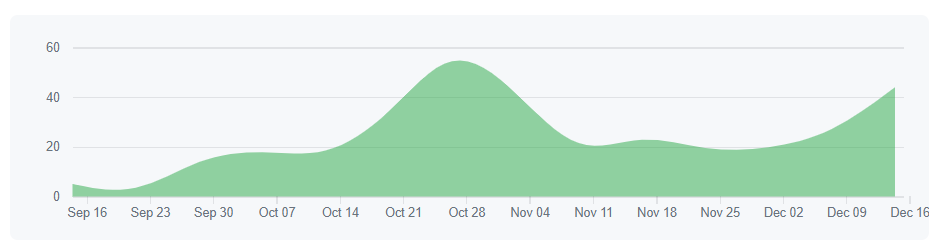
\includegraphics[width=150mm,scale=1]{githubproject.png}\\
In developing a timeline, our philosophy was to first implement some form of our hardest feature in our language, first-class functions, and then implement other features such as arrays and structs while we improved on our first-class function implementation. This method of creating the basic structure for first-class functions first before we added other features ensured that we didn’t have to read through large amounts of code while debugging issues with first-class functions. It also allowed us to constantly check that our implementations of other features worked correctly within first-class functions instead of forcing us to retroactively change our implementations to work correctly under closure principals. 

Additionally, we aimed to first get a working “Hello World” program to run in our language as quickly as we could to ensure that we meet the class deadlines. 

\subsubsection{Planned Timeline}
Sep 17 - goal of having language design finalized; \\
Project Proposal due Wed Sep 19; \\
LRM, Parser, AST due Mon Oct 15; \\
Oct 25th - goal of having a working Hello World; \\
Nov 14 - goal of having working first class functions;\\
Hello World due Wed Nov 14;\\
Nov 25th - goal of having working arrays, structs;\\
Dec 14 - goal of having testing complete;\\
Dec 17 - goal of having final report complete;\\
Project Reports due Wed Dec 19.\\
\\
\subsubsection{Actual Project Timeline}
Submitted project proposal Sept 19 for an overly ambitious language;\\
Oct 3 -- revisited and finalize general idea for our language;\\
Oct 14 -- first implementation of parser, AST, and tests for the parser was completed;\\
Oct. 27 -- first working “Hello World” with basic LLVM code;\\
Nov 6 -- first class functions mostly completed (with a few bugs);\\
Nov 11 -- structs mostly completed;\\
Nov 19 -- arrays mostly completed;\\
Dec 4 -- finished built-in functions;\\
Dec 14 - completed tests;\\
Dec 17 - completed final report;\\

\subsection{Team Roles and Responsibilities}
Claire Adams, Manager \\
Samurdha Jayasinghe, System Architect\\ 
Cindy Le, Language Guru\\
Crystal Ren, Test Designer

Every member of the team touched every file in the compiler and contributed to the test suite as well as the writing of the Language Reference Manual and Final Report. We assigned work based on the types specified in the AST, and it was expected that the person assigned to a type ensured that it worked all the way through to code generation. We often ended working together on implementing more complex features and resolving pesky bugs. \\

\begin{center}
\begin{tabular}{| c | c | }
   \hline
   Binary Operators & Cindy, Crystal \\
  \hline
   Unary Operators & Cindy \\
  \hline
Increment/Decrement Operators & Cindy \\
  \hline
   Structs & Claire, Sam \\
  \hline
  Arrays & Claire \\
  \hline
    Function Type & Sam \\
  \hline
    First-class Functions Lifter & Cindy, Claire, Crystal, Sam \\
  \hline
    Destructuring Assignment & Sam \\
  \hline
    Built-in Functions & Claire, Crystal \\
  \hline
    If-statements & Crystal \\
  \hline
    For and While loops & Cindy, Claire \\
  \hline
    Pretty-printer & Sam \\
  \hline
    Parser Test Suite setup & Crystal, Sam \\
  \hline
    Parser Test Suite tests & Cindy, Claire, Crystal, Sam \\
  \hline
    Integration Tests & Cindy, Claire, Crystal, Sam \\
  \hline
    Demo Code & Crystal, Cindy, Sam \\
  \hline
    Language Reference Manual & Cindy, Claire, Crystal, Sam \\
  \hline
    Final Report & Cindy, Claire, Crystal, Sam \\
  \hline
\end{tabular}
\end{center}

\subsection{Software Development Environment}
Libraries and Languages:
OCaml version 4.05.0; \\
OCaml LLVM version 6.0.0;\\
OCamlyacc version 4.05.0;\\
Ocamllex version 4.05.0.\\
C \& C libraries: stdio.h, stdlib.h, string.h, math.h, and time.h. \\

Software: A git repository on GitHub was used for version control of the code. LaTeX files on Overleaf were used to manage the project reports, such as the proposal, Language Reference Manual, and the final report. 

OS: Ubuntu 18.04.1 and MacOS 10.13.6 with Docker 2.0.0.0-mac81

\subsection{Project Log}
See Appendix 9.1 Project Log for all of our GitHub commit messages that show the course of our development. 

\section{Language Evolution}
This section records how Shoo's design has changed throughout the development and discusses the specific design choices we have made.

\subsection{Original Thoughts}
We originally envisioned Shoo as a less functionally robust version of Go with slightly more C-like syntax. 

Shoo was supposed to emulate Go in the way it spins off new threads via Shoo-routines, how pipes (message queues) are used to communicate between threads, and the inclusion of first class functions. 

Shoo-routines, our version of goroutines, execute in a separate thread, allowing for parallel programming. There were also supposed to be unnamed shoo-routines, where the return type is not required for an unnamed shoo-routine as the return value will be ignored.

The shoo keyword was also originally intended to run a named function in a separate thread. The function would have access to variables in the parent scope where it's defined. Any additional arguments may be passed in as parameters. 

The first draft of our LRM proposes features like spinning up threads, first-class functions, strings, initialized structs, polyxmorphic arrays and pipes, etc. that are (in hindsight) very complex.

We named the language Shoo-lang after the programming language Go-lang.

\subsection{Narrowing Down the Scope}

After talking to our project advisor, Justin, we narrowed down the scope. 

The difficulty did not occur in implementing any of these in isolation but to manage how all of these things are going to interact with each other in a multi-threaded environment. Interactions among the features that we proposed can become more complicated than we expected. For example, we should consider whether and how to include structs passed through pipes, arrays of locks, and so on. 

Therefore, we decided to get rid of the concurrent features. What we then end up with is a language with first-class functions, strings, structs, arrays, etc. limited to a single thread. 

Confident in our ability to implement first-class functions in a single threaded setting, we decided to keep the feature of first-class functions. It will make our language powerful in performing certain tasks and in general is a good feature to have.

\subsection{Design Choices for Syntax}

We first included single-line comments, declarative statements, for loops, chars and arrays, structs, if-else statements, and arithmetic \& logical operators. Later, we decided to include a ``new'' keyword for allocating structs and arrays, nested multi-line comments, and destructuring assignment of structs.

We realized the need for a dot operator so that we can have a function that returns a struct and then call .$<$fieldname$>$ on the returned struct.

We set up the parsing rule that struct ids should start with uppercase and regular variable ids should start with lowercase. Much of our later code depends on the rule, so we wanted to enforce it as a syntax rather than an optional style guideline.

We also have some syntactic sugar for the programmer's convenience, such as while loops and destructuring structs.

\subsection{Design Choices for Functionality}

Shoo has a very basic level of user-implementable polymorphism implicit in Shoo structs. For example, you can create a wrapper struct that can contain several different other structs and then set a flag to indicate which type of inner struct this wrapper struct should represent and so forth.

We decided not to include recursive struct definitions because of some time limitationes. Unfortunately, this means Shoo cannot support linked lists or trees that are implemented in the traditional way.

We decided to differentiate structs based on their name rather than based on the types of their members. Both have trade-offs. One advantage of disallowing identical members for different structs is that the compiler would be able to disambiguate struct types without having an explicit annotation of member maps.

We decided to have multi-dimensional arrays in Shoo so that it can perform a wider range of tasks. To initialize multi-dimensional arrays, one will need to initialize every element of the outermost level of the array. Then the multi-dimensional arrays will function just as expected.

Currently Shoo does not support enhanced for loops for arrays or strings. Due to time limitations, we did not get around to implementing a way of encoding lengths for arrays. For example, a workaround is to add another layer of indirection by putting each array inside a struct which contains the length of that array. 

\subsection{Design Summary}
We aimed at finding a balance between making the language easy to write and keeping the compiler work simple. Shoo does not do automatic garbage collection (or even C like garbage collection) and tries to simplify syntax as much as possible while still providing powerful features like first-class functions, structs, and multi-dimensional arrays.

\section{Translator Architecture}
The Shoo compiler consists of several modules that transform Shoo source code into a binary executable file, which is the flow shown below. All components, with the exception of the built-in functions, were worked on by everyone. Built-ins were done by Claire and Crystal.

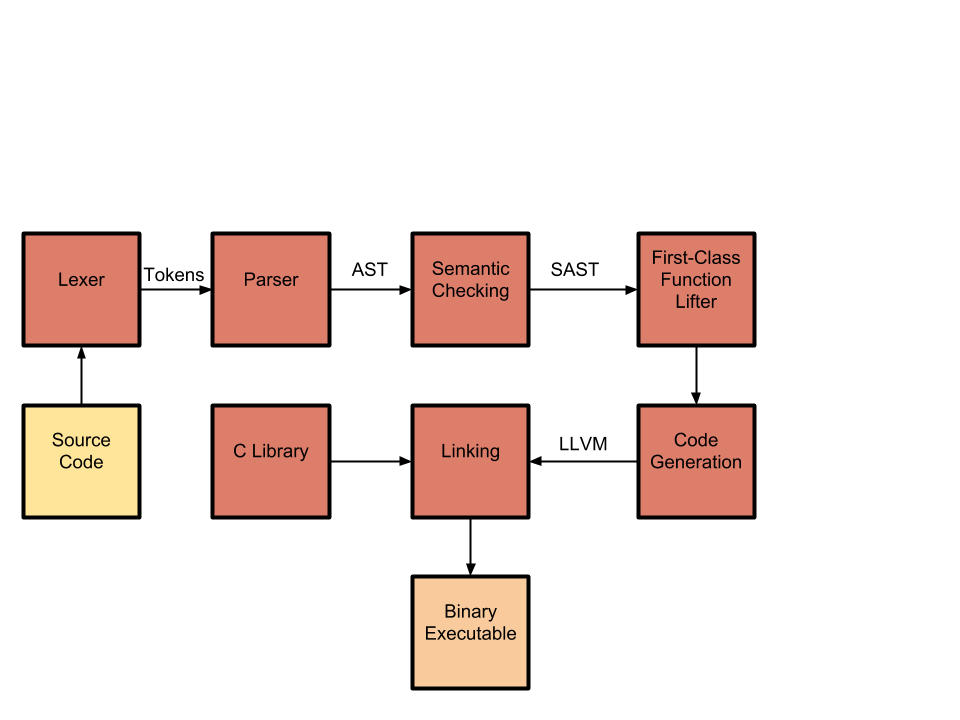
\includegraphics[width=100mm,scale=0.5]{design.png}

\subsection{Lexer}
The lexer (scanner.mll) takes in a Shoo source program of ASCII characters and translate them into tokens. If any characters in the code are detected to be illegal, lexing errors will be thrown. Characters inside the commented blocks will be ignored. The lexer produces tokens that will then be used by the parser in the next step of compilation. 

\subsection{Parser}
The parser (parser.mly) converts the tokens from the scanner to an abstract syntax tree (AST) based on Shoo's context-free grammar rules for syntax described in the Language Reference Manual. If any violations are detected, such as unmatched parentheses or missing semicolons, parser errors will be thrown. 

\subsection{Semantic Checking}
The semantic checker (semant.ml) recursively traverses the AST and converts it to a semantically-checked abstract syntax tree (SAST) consisting of objects. An environment record is used to map a string identifier to an object stack. If there are typing or scoping errors, messages will be printed to indicate the type of errors. For example, if variables are referenced before initialization or assigned a different type than what was declared, the semantic checker will generate errors.

\subsection{First Class Function Lifter}
Shoo supports first-class functions, meaning that it treats functions as first-class citizens just like variables. The first-class function lifter (lift.ml) takes a list of SAST statements and converts it into a map that maps from the function name to a node with more information about the function including its name, free variable list, return type, parameters, and function body. Function declarations are rearranged such that they appear to be global function declarations (or ``lifted'' as you will). Because pulling functions out of their original places can result in information loss of their original environments, environment information is stored and carried around along with each SAST node from the previous component.

\subsection{Code Generation}
As each part of the SAST is linked to specific LLVM modules, the code generation part (codegen.ml) produces LLVM code through a post-order traverse of the SAST tree.

The most challenging aspect of code generation was generating first class functions. Every function expression gets lifted as a closure to the global scope and is assigned a name based on a monotonically increasing counter.  The closure is allocated on the heap based on the struct implementation provided LLVM, because the closures are stored as LLVM structs (our particular implementation never frees...anything...ever). Consider the following sample program. The function expression returned by foo needs to be able to access the variable x even after the stack activation record for foo is replaced by the activation record for the call to baz. Because of this, we do not allocate the variable x on the stack. Instead, we allocate it on the heap such that the closure returned by foo can still reference the variable x. 

\begin{lstlisting}
function foo() func(;int) {
  int x = 5;
  return function () int  {
    return x;
  };
}

function baz() void {
  println("baz");
}

func(;int) bar = foo();
baz();
println(str_of_int(bar()));
\end{lstlisting}

We also implemented some features as syntactic sugar, such as destructuring assignment and while loops. If the semantic checker decides that a destructuring assignment is semantically correct, it will turn this statement into a series of statements, where the initial statement declares a temporary variable which holds the result of evaluating the right hand side expression and the subsequent series of statements will be variable declarations that get initialized by struct accesses on the temporary variable.
\\ \\
Arrays are implemented by mallocing the memory needed for the array and then returning the pointer to the malloc'd array. 
\\ \\
If the array contains composite types, the elements need to be initialized independently. Arrays initialized using new will not have any initialization performed on the elements. If the array is defined with literals, the items will already be initialized. For primitive types, the actual values will be stored, for composite types like structs, other arrays, strings, or functions, a reference to the element is stored instead of the value itself. 
\\ \\
Structs are implemented by mallocing the struct memory on the heap. If there are default values for the struct these values will also be allocated on the heap.

\subsection{C Libraries}
C libraries were linked in because we use C (and some C libraries like the math library) to write our built-in functions (src/builtins.c).

\section{Test Plan}
The end-to-end integration tests can be found in the test/ directory. The Unit Testing files for the parser described below are not included in our final submittion because we did not keep them up-to-date with the changes we made to the AST once we had the integration tests working.\\

\subsection{Unit Testing}
We had two phases of testing. Before we implemented any sort of codegen, we were working on the parser and the semantic checker, and had to do unit testing for the parser and semantic checker to make sure the source code fed to the scanner was parsed correctly by the parser and would be correct when we got codegen up and running. For these tests, we used OUnit2, OCaml's version of Java JUint designed to simplify the process of writing unit tests in OCaml, to compare the output of parsing code in our language to an expected output based on how we believed that the code should be parsed into the components outlined in the AST. These tests were later deleted once codegen was implemented, at which point we moved over into purely integration testing. \\

\subsection{Integration Tests}
The second phase of testing happened once we implemented code generation for our language. In this phase, we wrote an end-to-end integration test suite to rigorously test the functionality of our language as we implemented it. The test suite also ensured that we did not break previously working features when we added new ones. \\
\\
For the integration tests, all of the tests that should successfully produce output follow the naming pattern of using test-*.shoo for the test program and then using the same name but different file extension of the form test-*.out for the expected output of the program. All of the negative tests similarly used fail-*.shoo for the test program that should fail and used fail-*.err instead of .out for the expected error message. \\
\\
A complete set of tests can be found in Appendix 10.14 Integration Tests Files (Negative tests) and Appendix 10.15 Integration Tests Files (Positive tests).\\
These tests were implemented mostly in parallel with the functionality they tested and so they were chosen to test the implemented functionality and failure cases of the implemented functionality.
\\
All members of the team worked on various tests of the test suite. We did not individually mark the authors of each individual test (there are over 100 of them) but each person added many tests.

\subsubsection{Test Automation and Scripts}
For our integration tests, we used a modified version of the testall.sh script provided by Professor Edwards for the MicroC compiler. It prints a line to the screen once it finishes running the full test suite summarizing the number of passing test cases. The script works by running all of the test-*.shoo and fail-*.shoo programs and then comparing the outputs or errors respectively to see if they match the expected value. If the output or error fails to match what is expected, the script will print out FAILED next to the test name along with an error message. A more detailed error message can be found by looking in testall.log. If the test is successful, the script prints a `.' instead of printing the test name. Only failing test names are printed. This way the script output is less verbose and easier to read. \\
\\
For larger end-to-end tests, (ie. sample programs), we created a separate directory called sample\textunderscore programs to hold these programs. These tests can be run using the run.sh script, which takes the file path to the program to run as an argument.\\
Example:\\
\begin{lstlisting}
./run.sh sample_programs/demo1.shoo
\end{lstlisting}

testall.sh and run.sh can be found in Appendix 10.12 testall.sh and Appendix 10.13 run.sh respectively. \\
\\

\subsection{Example Test Programs}
\\
Shoo Code 1:\\
\\
\begin{mdframed}[hidealllines=true,backgroundcolor=blue!10]
\begin{lstlisting}
struct Object {
	int index;
	int data;
}

function compareData(Object a, Object b) bool {
    return a.data < b.data;
}

function compareIndex(Object a, Object b) bool {
    return a.index < b.index;
}

function printData(array<Object> arr, int n) void {
	for (int i = 0; i < n; i++) {
		println(str_of_int(arr[i].data));
	}
	
	return;
}

function printIndex(array<Object> arr, int n) void {
	for (int i = 0; i < n; i++) {
		println(str_of_int(arr[i].index));
	}
	
	return;
}

function bubbleSort(array<Object> arr, int n, func(Object, Object; bool) compare) array<Object> {
	for (int i = 0; i < n - 1; i++) {
		for (int j = 0; j < n - i - 1; j++) {
			if (compare(arr[j + 1], arr[j])) {
				Object temp = arr[j];
				arr[j] = arr[j + 1];
				arr[j + 1] = temp;
			}
		}
	}
	
	return arr;
}

array<int> indices = [1,3,8,6,9,7,0,2,4,5];
array<int> datapoints = [106,101,104,108,105,103,102,109,107,100];

int n = 10;
array<Object> objects = new(array<Object>[n]);

for (int i = 0; i < n; i++) {
	objects[i] = new(Object);
	objects[i].index = indices[i]; 
	objects[i].data = datapoints[i];
}

printIndex(objects, n);
printData(objects, n);

bubbleSort(objects, n, compareIndex);
printIndex(objects, n);

bubbleSort(objects, n, compareData);
printData(objects, n);

\end{lstlisting}
\end{mdframed}
\\
LLVM Code 1:\\
\\
\begin{mdframed}[hidealllines=true,backgroundcolor=green!10]
\begin{lstlisting}
; ModuleID = 'Shoo'
source_filename = "Shoo"

declare void @println(i8*)

declare void @print(i8*)

declare i8* @str_of_int(i32)

declare i8* @str_of_bool(i1)

declare i8* @string_concat(i8*, i8*)

declare i32 @string_equals(i8*, i8*)

declare i8* @str_of_float(double)

declare i32 @int_of_float(double)

declare double @float_of_int(i32)

declare i8* @scan_line(i32)

declare void @exit_success()

declare void @die(i8*, i32)

declare i32 @int_of_str(i8*)

declare void @rand_autoseed()

declare i32 @rand_afterseed()

declare i8* @scan_char()

define i32 @main() {
entry:
  %malloccall = tail call i8* @malloc(i32 ptrtoint (i1** getelementptr (i1*, i1** null, i32 1) to i32))
  %env = bitcast i8* %malloccall to i8**
  store i8* null, i8** %env
  %env_p = load i8*, i8** %env
  %malloccall1 = tail call i8* @malloc(i32 trunc (i64 mul nuw (i64 ptrtoint (i1** getelementptr (i1*, i1** null, i32 1) to i64), i64 2) to i32))
  %main = bitcast i8* %malloccall1 to { i32 ()*, i8* }*
  %tmp__ = insertvalue { i32 ()*, i8* } { i32 ()* @main, i8* null }, i8* %env_p, 1
  store { i32 ()*, i8* } %tmp__, { i32 ()*, i8* }* %main
  %malloccall2 = tail call i8* @malloc(i32 trunc (i64 mul nuw (i64 ptrtoint (i1** getelementptr (i1*, i1** null, i32 1) to i64), i64 2) to i32))
  %compareData = bitcast i8* %malloccall2 to { i1 (i8*, { i32, i32 }*, { i32, i32 }*)*, i8* }*
  %malloccall3 = tail call i8* @malloc(i32 0)
  %tmp_ = bitcast i8* %malloccall3 to {}*
  store {} zeroinitializer, {}* %tmp_
  %env_p4 = bitcast {}* %tmp_ to i8*
  %tmp__5 = insertvalue { i1 (i8*, { i32, i32 }*, { i32, i32 }*)*, i8* } { i1 (i8*, { i32, i32 }*, { i32, i32 }*)* @f0, i8* null }, i8* %env_p4, 1
  store { i1 (i8*, { i32, i32 }*, { i32, i32 }*)*, i8* } %tmp__5, { i1 (i8*, { i32, i32 }*, { i32, i32 }*)*, i8* }* %compareData
  %malloccall6 = tail call i8* @malloc(i32 trunc (i64 mul nuw (i64 ptrtoint (i1** getelementptr (i1*, i1** null, i32 1) to i64), i64 2) to i32))
  %compareIndex = bitcast i8* %malloccall6 to { i1 (i8*, { i32, i32 }*, { i32, i32 }*)*, i8* }*
  %malloccall7 = tail call i8* @malloc(i32 0)
  %tmp_8 = bitcast i8* %malloccall7 to {}*
  store {} zeroinitializer, {}* %tmp_8
  %env_p9 = bitcast {}* %tmp_8 to i8*
  %tmp__10 = insertvalue { i1 (i8*, { i32, i32 }*, { i32, i32 }*)*, i8* } { i1 (i8*, { i32, i32 }*, { i32, i32 }*)* @f1, i8* null }, i8* %env_p9, 1
  store { i1 (i8*, { i32, i32 }*, { i32, i32 }*)*, i8* } %tmp__10, { i1 (i8*, { i32, i32 }*, { i32, i32 }*)*, i8* }* %compareIndex
  %malloccall11 = tail call i8* @malloc(i32 trunc (i64 mul nuw (i64 ptrtoint (i1** getelementptr (i1*, i1** null, i32 1) to i64), i64 2) to i32))
  %printData = bitcast i8* %malloccall11 to { void (i8*, { i32, i32 }**, i32)*, i8* }*
  %malloccall12 = tail call i8* @malloc(i32 0)
  %tmp_13 = bitcast i8* %malloccall12 to {}*
  store {} zeroinitializer, {}* %tmp_13
  %env_p14 = bitcast {}* %tmp_13 to i8*
  %tmp__15 = insertvalue { void (i8*, { i32, i32 }**, i32)*, i8* } { void (i8*, { i32, i32 }**, i32)* @f2, i8* null }, i8* %env_p14, 1
  store { void (i8*, { i32, i32 }**, i32)*, i8* } %tmp__15, { void (i8*, { i32, i32 }**, i32)*, i8* }* %printData
  %malloccall16 = tail call i8* @malloc(i32 trunc (i64 mul nuw (i64 ptrtoint (i1** getelementptr (i1*, i1** null, i32 1) to i64), i64 2) to i32))
  %printIndex = bitcast i8* %malloccall16 to { void (i8*, { i32, i32 }**, i32)*, i8* }*
  %malloccall17 = tail call i8* @malloc(i32 0)
  %tmp_18 = bitcast i8* %malloccall17 to {}*
  store {} zeroinitializer, {}* %tmp_18
  %env_p19 = bitcast {}* %tmp_18 to i8*
  %tmp__20 = insertvalue { void (i8*, { i32, i32 }**, i32)*, i8* } { void (i8*, { i32, i32 }**, i32)* @f3, i8* null }, i8* %env_p19, 1
  store { void (i8*, { i32, i32 }**, i32)*, i8* } %tmp__20, { void (i8*, { i32, i32 }**, i32)*, i8* }* %printIndex
  %malloccall21 = tail call i8* @malloc(i32 trunc (i64 mul nuw (i64 ptrtoint (i1** getelementptr (i1*, i1** null, i32 1) to i64), i64 2) to i32))
  %bubbleSort = bitcast i8* %malloccall21 to { { i32, i32 }** (i8*, { i32, i32 }**, i32, { i1 (i8*, { i32, i32 }*, { i32, i32 }*)*, i8* })*, i8* }*
  %malloccall22 = tail call i8* @malloc(i32 0)
  %tmp_23 = bitcast i8* %malloccall22 to {}*
  store {} zeroinitializer, {}* %tmp_23
  %env_p24 = bitcast {}* %tmp_23 to i8*
  %tmp__25 = insertvalue { { i32, i32 }** (i8*, { i32, i32 }**, i32, { i1 (i8*, { i32, i32 }*, { i32, i32 }*)*, i8* })*, i8* } { { i32, i32 }** (i8*, { i32, i32 }**, i32, { i1 (i8*, { i32, i32 }*, { i32, i32 }*)*, i8* })* @f4, i8* null }, i8* %env_p24, 1
  store { { i32, i32 }** (i8*, { i32, i32 }**, i32, { i1 (i8*, { i32, i32 }*, { i32, i32 }*)*, i8* })*, i8* } %tmp__25, { { i32, i32 }** (i8*, { i32, i32 }**, i32, { i1 (i8*, { i32, i32 }*, { i32, i32 }*)*, i8* })*, i8* }* %bubbleSort
  %malloccall26 = tail call i8* @malloc(i32 ptrtoint (i1** getelementptr (i1*, i1** null, i32 1) to i32))
  %indices = bitcast i8* %malloccall26 to i32**
  %malloccall27 = tail call i8* @malloc(i32 mul (i32 ptrtoint (i32* getelementptr (i32, i32* null, i32 1) to i32), i32 10))
  %0 = bitcast i8* %malloccall27 to i32*
  %1 = getelementptr i32, i32* %0, i32 0
  store i32 1, i32* %1
  %2 = getelementptr i32, i32* %0, i32 1
  store i32 3, i32* %2
  %3 = getelementptr i32, i32* %0, i32 2
  store i32 8, i32* %3
  %4 = getelementptr i32, i32* %0, i32 3
  store i32 6, i32* %4
  %5 = getelementptr i32, i32* %0, i32 4
  store i32 9, i32* %5
  %6 = getelementptr i32, i32* %0, i32 5
  store i32 7, i32* %6
  %7 = getelementptr i32, i32* %0, i32 6
  store i32 0, i32* %7
  %8 = getelementptr i32, i32* %0, i32 7
  store i32 2, i32* %8
  %9 = getelementptr i32, i32* %0, i32 8
  store i32 4, i32* %9
  %10 = getelementptr i32, i32* %0, i32 9
  store i32 5, i32* %10
  store i32* %0, i32** %indices
  %malloccall28 = tail call i8* @malloc(i32 ptrtoint (i1** getelementptr (i1*, i1** null, i32 1) to i32))
  %datapoints = bitcast i8* %malloccall28 to i32**
  %malloccall29 = tail call i8* @malloc(i32 mul (i32 ptrtoint (i32* getelementptr (i32, i32* null, i32 1) to i32), i32 10))
  %11 = bitcast i8* %malloccall29 to i32*
  %12 = getelementptr i32, i32* %11, i32 0
  store i32 106, i32* %12
  %13 = getelementptr i32, i32* %11, i32 1
  store i32 101, i32* %13
  %14 = getelementptr i32, i32* %11, i32 2
  store i32 104, i32* %14
  %15 = getelementptr i32, i32* %11, i32 3
  store i32 108, i32* %15
  %16 = getelementptr i32, i32* %11, i32 4
  store i32 105, i32* %16
  %17 = getelementptr i32, i32* %11, i32 5
  store i32 103, i32* %17
  %18 = getelementptr i32, i32* %11, i32 6
  store i32 102, i32* %18
  %19 = getelementptr i32, i32* %11, i32 7
  store i32 109, i32* %19
  %20 = getelementptr i32, i32* %11, i32 8
  store i32 107, i32* %20
  %21 = getelementptr i32, i32* %11, i32 9
  store i32 100, i32* %21
  store i32* %11, i32** %datapoints
  %malloccall30 = tail call i8* @malloc(i32 ptrtoint (i32* getelementptr (i32, i32* null, i32 1) to i32))
  %n = bitcast i8* %malloccall30 to i32*
  store i32 10, i32* %n
  %malloccall31 = tail call i8* @malloc(i32 ptrtoint (i1** getelementptr (i1*, i1** null, i32 1) to i32))
  %objects = bitcast i8* %malloccall31 to { i32, i32 }***
  %n32 = load i32, i32* %n
  %mallocsize = mul i32 %n32, ptrtoint (i1** getelementptr (i1*, i1** null, i32 1) to i32)
  %malloccall33 = tail call i8* @malloc(i32 %mallocsize)
  %22 = bitcast i8* %malloccall33 to { i32, i32 }**
  store { i32, i32 }** %22, { i32, i32 }*** %objects
  br label %init_loop

init_loop:                                        ; preds = %entry
  %malloccall34 = tail call i8* @malloc(i32 ptrtoint (i32* getelementptr (i32, i32* null, i32 1) to i32))
  %i = bitcast i8* %malloccall34 to i32*
  store i32 0, i32* %i
  br label %for

for:                                              ; preds = %for_body, %init_loop
  %i48 = load i32, i32* %i
  %n49 = load i32, i32* %n
  %tmp50 = icmp slt i32 %i48, %n49
  br i1 %tmp50, label %for_body, label %merge

for_body:                                         ; preds = %for
  %malloccall35 = tail call i8* @malloc(i32 trunc (i64 mul nuw (i64 ptrtoint (i32* getelementptr (i32, i32* null, i32 1) to i64), i64 2) to i32))
  %structlit = bitcast i8* %malloccall35 to { i32, i32 }*
  store { i32, i32 } zeroinitializer, { i32, i32 }* %structlit
  %objects36 = load { i32, i32 }**, { i32, i32 }*** %objects
  %i37 = load i32, i32* %i
  %23 = getelementptr { i32, i32 }*, { i32, i32 }** %objects36, i32 %i37
  store { i32, i32 }* %structlit, { i32, i32 }** %23
  %indices38 = load i32*, i32** %indices
  %i39 = load i32, i32* %i
  %24 = getelementptr i32, i32* %indices38, i32 %i39
  %25 = load i32, i32* %24
  %objects40 = load { i32, i32 }**, { i32, i32 }*** %objects
  %i41 = load i32, i32* %i
  %26 = getelementptr { i32, i32 }*, { i32, i32 }** %objects40, i32 %i41
  %27 = load { i32, i32 }*, { i32, i32 }** %26
  %structval = load { i32, i32 }, { i32, i32 }* %27
  %index = insertvalue { i32, i32 } %structval, i32 %25, 1
  store { i32, i32 } %index, { i32, i32 }* %27
  %datapoints42 = load i32*, i32** %datapoints
  %i43 = load i32, i32* %i
  %28 = getelementptr i32, i32* %datapoints42, i32 %i43
  %29 = load i32, i32* %28
  %objects44 = load { i32, i32 }**, { i32, i32 }*** %objects
  %i45 = load i32, i32* %i
  %30 = getelementptr { i32, i32 }*, { i32, i32 }** %objects44, i32 %i45
  %31 = load { i32, i32 }*, { i32, i32 }** %30
  %structval46 = load { i32, i32 }, { i32, i32 }* %31
  %data = insertvalue { i32, i32 } %structval46, i32 %29, 0
  store { i32, i32 } %data, { i32, i32 }* %31
  %i47 = load i32, i32* %i
  %tmp = add i32 %i47, 1
  store i32 %tmp, i32* %i
  br label %for

merge:                                            ; preds = %for
  %printIndex51 = load { void (i8*, { i32, i32 }**, i32)*, i8* }, { void (i8*, { i32, i32 }**, i32)*, i8* }* %printIndex
  %fp = extractvalue { void (i8*, { i32, i32 }**, i32)*, i8* } %printIndex51, 0
  %envp = extractvalue { void (i8*, { i32, i32 }**, i32)*, i8* } %printIndex51, 1
  %n52 = load i32, i32* %n
  %objects53 = load { i32, i32 }**, { i32, i32 }*** %objects
  call void %fp(i8* %envp, { i32, i32 }** %objects53, i32 %n52)
  %printData54 = load { void (i8*, { i32, i32 }**, i32)*, i8* }, { void (i8*, { i32, i32 }**, i32)*, i8* }* %printData
  %fp55 = extractvalue { void (i8*, { i32, i32 }**, i32)*, i8* } %printData54, 0
  %envp56 = extractvalue { void (i8*, { i32, i32 }**, i32)*, i8* } %printData54, 1
  %n57 = load i32, i32* %n
  %objects58 = load { i32, i32 }**, { i32, i32 }*** %objects
  call void %fp55(i8* %envp56, { i32, i32 }** %objects58, i32 %n57)
  %bubbleSort59 = load { { i32, i32 }** (i8*, { i32, i32 }**, i32, { i1 (i8*, { i32, i32 }*, { i32, i32 }*)*, i8* })*, i8* }, { { i32, i32 }** (i8*, { i32, i32 }**, i32, { i1 (i8*, { i32, i32 }*, { i32, i32 }*)*, i8* })*, i8* }* %bubbleSort
  %fp60 = extractvalue { { i32, i32 }** (i8*, { i32, i32 }**, i32, { i1 (i8*, { i32, i32 }*, { i32, i32 }*)*, i8* })*, i8* } %bubbleSort59, 0
  %envp61 = extractvalue { { i32, i32 }** (i8*, { i32, i32 }**, i32, { i1 (i8*, { i32, i32 }*, { i32, i32 }*)*, i8* })*, i8* } %bubbleSort59, 1
  %compareIndex62 = load { i1 (i8*, { i32, i32 }*, { i32, i32 }*)*, i8* }, { i1 (i8*, { i32, i32 }*, { i32, i32 }*)*, i8* }* %compareIndex
  %n63 = load i32, i32* %n
  %objects64 = load { i32, i32 }**, { i32, i32 }*** %objects
  %_result = call { i32, i32 }** %fp60(i8* %envp61, { i32, i32 }** %objects64, i32 %n63, { i1 (i8*, { i32, i32 }*, { i32, i32 }*)*, i8* } %compareIndex62)
  %printIndex65 = load { void (i8*, { i32, i32 }**, i32)*, i8* }, { void (i8*, { i32, i32 }**, i32)*, i8* }* %printIndex
  %fp66 = extractvalue { void (i8*, { i32, i32 }**, i32)*, i8* } %printIndex65, 0
  %envp67 = extractvalue { void (i8*, { i32, i32 }**, i32)*, i8* } %printIndex65, 1
  %n68 = load i32, i32* %n
  %objects69 = load { i32, i32 }**, { i32, i32 }*** %objects
  call void %fp66(i8* %envp67, { i32, i32 }** %objects69, i32 %n68)
  %bubbleSort70 = load { { i32, i32 }** (i8*, { i32, i32 }**, i32, { i1 (i8*, { i32, i32 }*, { i32, i32 }*)*, i8* })*, i8* }, { { i32, i32 }** (i8*, { i32, i32 }**, i32, { i1 (i8*, { i32, i32 }*, { i32, i32 }*)*, i8* })*, i8* }* %bubbleSort
  %fp71 = extractvalue { { i32, i32 }** (i8*, { i32, i32 }**, i32, { i1 (i8*, { i32, i32 }*, { i32, i32 }*)*, i8* })*, i8* } %bubbleSort70, 0
  %envp72 = extractvalue { { i32, i32 }** (i8*, { i32, i32 }**, i32, { i1 (i8*, { i32, i32 }*, { i32, i32 }*)*, i8* })*, i8* } %bubbleSort70, 1
  %compareData73 = load { i1 (i8*, { i32, i32 }*, { i32, i32 }*)*, i8* }, { i1 (i8*, { i32, i32 }*, { i32, i32 }*)*, i8* }* %compareData
  %n74 = load i32, i32* %n
  %objects75 = load { i32, i32 }**, { i32, i32 }*** %objects
  %_result76 = call { i32, i32 }** %fp71(i8* %envp72, { i32, i32 }** %objects75, i32 %n74, { i1 (i8*, { i32, i32 }*, { i32, i32 }*)*, i8* } %compareData73)
  %printData77 = load { void (i8*, { i32, i32 }**, i32)*, i8* }, { void (i8*, { i32, i32 }**, i32)*, i8* }* %printData
  %fp78 = extractvalue { void (i8*, { i32, i32 }**, i32)*, i8* } %printData77, 0
  %envp79 = extractvalue { void (i8*, { i32, i32 }**, i32)*, i8* } %printData77, 1
  %n80 = load i32, i32* %n
  %objects81 = load { i32, i32 }**, { i32, i32 }*** %objects
  call void %fp78(i8* %envp79, { i32, i32 }** %objects81, i32 %n80)
  ret i32 0
}

define i1 @f0(i8* %env, { i32, i32 }* %a, { i32, i32 }* %b) {
entry:
  %malloccall = tail call i8* @malloc(i32 ptrtoint (i1** getelementptr (i1*, i1** null, i32 1) to i32))
  %a1 = bitcast i8* %malloccall to { i32, i32 }**
  store { i32, i32 }* %a, { i32, i32 }** %a1
  %malloccall2 = tail call i8* @malloc(i32 ptrtoint (i1** getelementptr (i1*, i1** null, i32 1) to i32))
  %b3 = bitcast i8* %malloccall2 to { i32, i32 }**
  store { i32, i32 }* %b, { i32, i32 }** %b3
  %malloccall4 = tail call i8* @malloc(i32 ptrtoint (i1** getelementptr (i1*, i1** null, i32 1) to i32))
  %env5 = bitcast i8* %malloccall4 to i8**
  store i8* %env, i8** %env5
  %env_p = load i8*, i8** %env5
  %malloccall6 = tail call i8* @malloc(i32 trunc (i64 mul nuw (i64 ptrtoint (i1** getelementptr (i1*, i1** null, i32 1) to i64), i64 2) to i32))
  %compareData = bitcast i8* %malloccall6 to { i1 (i8*, { i32, i32 }*, { i32, i32 }*)*, i8* }*
  %tmp__ = insertvalue { i1 (i8*, { i32, i32 }*, { i32, i32 }*)*, i8* } { i1 (i8*, { i32, i32 }*, { i32, i32 }*)* @f0, i8* null }, i8* %env_p, 1
  store { i1 (i8*, { i32, i32 }*, { i32, i32 }*)*, i8* } %tmp__, { i1 (i8*, { i32, i32 }*, { i32, i32 }*)*, i8* }* %compareData
  %a7 = load { i32, i32 }*, { i32, i32 }** %a1
  %structval = load { i32, i32 }, { i32, i32 }* %a7
  %data = extractvalue { i32, i32 } %structval, 0
  %b8 = load { i32, i32 }*, { i32, i32 }** %b3
  %structval9 = load { i32, i32 }, { i32, i32 }* %b8
  %data10 = extractvalue { i32, i32 } %structval9, 0
  %tmp = icmp slt i32 %data, %data10
  ret i1 %tmp
}

define i1 @f1(i8* %env, { i32, i32 }* %a, { i32, i32 }* %b) {
entry:
  %malloccall = tail call i8* @malloc(i32 ptrtoint (i1** getelementptr (i1*, i1** null, i32 1) to i32))
  %a1 = bitcast i8* %malloccall to { i32, i32 }**
  store { i32, i32 }* %a, { i32, i32 }** %a1
  %malloccall2 = tail call i8* @malloc(i32 ptrtoint (i1** getelementptr (i1*, i1** null, i32 1) to i32))
  %b3 = bitcast i8* %malloccall2 to { i32, i32 }**
  store { i32, i32 }* %b, { i32, i32 }** %b3
  %malloccall4 = tail call i8* @malloc(i32 ptrtoint (i1** getelementptr (i1*, i1** null, i32 1) to i32))
  %env5 = bitcast i8* %malloccall4 to i8**
  store i8* %env, i8** %env5
  %env_p = load i8*, i8** %env5
  %malloccall6 = tail call i8* @malloc(i32 trunc (i64 mul nuw (i64 ptrtoint (i1** getelementptr (i1*, i1** null, i32 1) to i64), i64 2) to i32))
  %compareIndex = bitcast i8* %malloccall6 to { i1 (i8*, { i32, i32 }*, { i32, i32 }*)*, i8* }*
  %tmp__ = insertvalue { i1 (i8*, { i32, i32 }*, { i32, i32 }*)*, i8* } { i1 (i8*, { i32, i32 }*, { i32, i32 }*)* @f1, i8* null }, i8* %env_p, 1
  store { i1 (i8*, { i32, i32 }*, { i32, i32 }*)*, i8* } %tmp__, { i1 (i8*, { i32, i32 }*, { i32, i32 }*)*, i8* }* %compareIndex
  %a7 = load { i32, i32 }*, { i32, i32 }** %a1
  %structval = load { i32, i32 }, { i32, i32 }* %a7
  %index = extractvalue { i32, i32 } %structval, 1
  %b8 = load { i32, i32 }*, { i32, i32 }** %b3
  %structval9 = load { i32, i32 }, { i32, i32 }* %b8
  %index10 = extractvalue { i32, i32 } %structval9, 1
  %tmp = icmp slt i32 %index, %index10
  ret i1 %tmp
}

define void @f2(i8* %env, { i32, i32 }** %arr, i32 %n) {
entry:
  %malloccall = tail call i8* @malloc(i32 ptrtoint (i1** getelementptr (i1*, i1** null, i32 1) to i32))
  %arr1 = bitcast i8* %malloccall to { i32, i32 }***
  store { i32, i32 }** %arr, { i32, i32 }*** %arr1
  %malloccall2 = tail call i8* @malloc(i32 ptrtoint (i32* getelementptr (i32, i32* null, i32 1) to i32))
  %n3 = bitcast i8* %malloccall2 to i32*
  store i32 %n, i32* %n3
  %malloccall4 = tail call i8* @malloc(i32 ptrtoint (i1** getelementptr (i1*, i1** null, i32 1) to i32))
  %env5 = bitcast i8* %malloccall4 to i8**
  store i8* %env, i8** %env5
  %env_p = load i8*, i8** %env5
  %malloccall6 = tail call i8* @malloc(i32 trunc (i64 mul nuw (i64 ptrtoint (i1** getelementptr (i1*, i1** null, i32 1) to i64), i64 2) to i32))
  %printData = bitcast i8* %malloccall6 to { void (i8*, { i32, i32 }**, i32)*, i8* }*
  %tmp__ = insertvalue { void (i8*, { i32, i32 }**, i32)*, i8* } { void (i8*, { i32, i32 }**, i32)* @f2, i8* null }, i8* %env_p, 1
  store { void (i8*, { i32, i32 }**, i32)*, i8* } %tmp__, { void (i8*, { i32, i32 }**, i32)*, i8* }* %printData
  br label %init_loop

init_loop:                                        ; preds = %entry
  %malloccall7 = tail call i8* @malloc(i32 ptrtoint (i32* getelementptr (i32, i32* null, i32 1) to i32))
  %i = bitcast i8* %malloccall7 to i32*
  store i32 0, i32* %i
  br label %for

for:                                              ; preds = %for_body, %init_loop
  %i11 = load i32, i32* %i
  %n12 = load i32, i32* %n3
  %tmp13 = icmp slt i32 %i11, %n12
  br i1 %tmp13, label %for_body, label %merge

for_body:                                         ; preds = %for
  %arr8 = load { i32, i32 }**, { i32, i32 }*** %arr1
  %i9 = load i32, i32* %i
  %0 = getelementptr { i32, i32 }*, { i32, i32 }** %arr8, i32 %i9
  %1 = load { i32, i32 }*, { i32, i32 }** %0
  %structval = load { i32, i32 }, { i32, i32 }* %1
  %data = extractvalue { i32, i32 } %structval, 0
  %_result = call i8* @str_of_int(i32 %data)
  call void @println(i8* %_result)
  %i10 = load i32, i32* %i
  %tmp = add i32 %i10, 1
  store i32 %tmp, i32* %i
  br label %for

merge:                                            ; preds = %for
  ret void
}

define void @f3(i8* %env, { i32, i32 }** %arr, i32 %n) {
entry:
  %malloccall = tail call i8* @malloc(i32 ptrtoint (i1** getelementptr (i1*, i1** null, i32 1) to i32))
  %arr1 = bitcast i8* %malloccall to { i32, i32 }***
  store { i32, i32 }** %arr, { i32, i32 }*** %arr1
  %malloccall2 = tail call i8* @malloc(i32 ptrtoint (i32* getelementptr (i32, i32* null, i32 1) to i32))
  %n3 = bitcast i8* %malloccall2 to i32*
  store i32 %n, i32* %n3
  %malloccall4 = tail call i8* @malloc(i32 ptrtoint (i1** getelementptr (i1*, i1** null, i32 1) to i32))
  %env5 = bitcast i8* %malloccall4 to i8**
  store i8* %env, i8** %env5
  %env_p = load i8*, i8** %env5
  %malloccall6 = tail call i8* @malloc(i32 trunc (i64 mul nuw (i64 ptrtoint (i1** getelementptr (i1*, i1** null, i32 1) to i64), i64 2) to i32))
  %printIndex = bitcast i8* %malloccall6 to { void (i8*, { i32, i32 }**, i32)*, i8* }*
  %tmp__ = insertvalue { void (i8*, { i32, i32 }**, i32)*, i8* } { void (i8*, { i32, i32 }**, i32)* @f3, i8* null }, i8* %env_p, 1
  store { void (i8*, { i32, i32 }**, i32)*, i8* } %tmp__, { void (i8*, { i32, i32 }**, i32)*, i8* }* %printIndex
  br label %init_loop

init_loop:                                        ; preds = %entry
  %malloccall7 = tail call i8* @malloc(i32 ptrtoint (i32* getelementptr (i32, i32* null, i32 1) to i32))
  %i = bitcast i8* %malloccall7 to i32*
  store i32 0, i32* %i
  br label %for

for:                                              ; preds = %for_body, %init_loop
  %i11 = load i32, i32* %i
  %n12 = load i32, i32* %n3
  %tmp13 = icmp slt i32 %i11, %n12
  br i1 %tmp13, label %for_body, label %merge

for_body:                                         ; preds = %for
  %arr8 = load { i32, i32 }**, { i32, i32 }*** %arr1
  %i9 = load i32, i32* %i
  %0 = getelementptr { i32, i32 }*, { i32, i32 }** %arr8, i32 %i9
  %1 = load { i32, i32 }*, { i32, i32 }** %0
  %structval = load { i32, i32 }, { i32, i32 }* %1
  %index = extractvalue { i32, i32 } %structval, 1
  %_result = call i8* @str_of_int(i32 %index)
  call void @println(i8* %_result)
  %i10 = load i32, i32* %i
  %tmp = add i32 %i10, 1
  store i32 %tmp, i32* %i
  br label %for

merge:                                            ; preds = %for
  ret void
}

define { i32, i32 }** @f4(i8* %env, { i32, i32 }** %arr, i32 %n, { i1 (i8*, { i32, i32 }*, { i32, i32 }*)*, i8* } %compare) {
entry:
  %malloccall = tail call i8* @malloc(i32 ptrtoint (i1** getelementptr (i1*, i1** null, i32 1) to i32))
  %arr1 = bitcast i8* %malloccall to { i32, i32 }***
  store { i32, i32 }** %arr, { i32, i32 }*** %arr1
  %malloccall2 = tail call i8* @malloc(i32 ptrtoint (i32* getelementptr (i32, i32* null, i32 1) to i32))
  %n3 = bitcast i8* %malloccall2 to i32*
  store i32 %n, i32* %n3
  %malloccall4 = tail call i8* @malloc(i32 trunc (i64 mul nuw (i64 ptrtoint (i1** getelementptr (i1*, i1** null, i32 1) to i64), i64 2) to i32))
  %compare5 = bitcast i8* %malloccall4 to { i1 (i8*, { i32, i32 }*, { i32, i32 }*)*, i8* }*
  store { i1 (i8*, { i32, i32 }*, { i32, i32 }*)*, i8* } %compare, { i1 (i8*, { i32, i32 }*, { i32, i32 }*)*, i8* }* %compare5
  %malloccall6 = tail call i8* @malloc(i32 ptrtoint (i1** getelementptr (i1*, i1** null, i32 1) to i32))
  %env7 = bitcast i8* %malloccall6 to i8**
  store i8* %env, i8** %env7
  %env_p = load i8*, i8** %env7
  %malloccall8 = tail call i8* @malloc(i32 trunc (i64 mul nuw (i64 ptrtoint (i1** getelementptr (i1*, i1** null, i32 1) to i64), i64 2) to i32))
  %bubbleSort = bitcast i8* %malloccall8 to { { i32, i32 }** (i8*, { i32, i32 }**, i32, { i1 (i8*, { i32, i32 }*, { i32, i32 }*)*, i8* })*, i8* }*
  %tmp__ = insertvalue { { i32, i32 }** (i8*, { i32, i32 }**, i32, { i1 (i8*, { i32, i32 }*, { i32, i32 }*)*, i8* })*, i8* } { { i32, i32 }** (i8*, { i32, i32 }**, i32, { i1 (i8*, { i32, i32 }*, { i32, i32 }*)*, i8* })* @f4, i8* null }, i8* %env_p, 1
  store { { i32, i32 }** (i8*, { i32, i32 }**, i32, { i1 (i8*, { i32, i32 }*, { i32, i32 }*)*, i8* })*, i8* } %tmp__, { { i32, i32 }** (i8*, { i32, i32 }**, i32, { i1 (i8*, { i32, i32 }*, { i32, i32 }*)*, i8* })*, i8* }* %bubbleSort
  br label %init_loop

init_loop:                                        ; preds = %entry
  %malloccall9 = tail call i8* @malloc(i32 ptrtoint (i32* getelementptr (i32, i32* null, i32 1) to i32))
  %i = bitcast i8* %malloccall9 to i32*
  store i32 0, i32* %i
  br label %for

for:                                              ; preds = %merge39, %init_loop
  %i42 = load i32, i32* %i
  %n43 = load i32, i32* %n3
  %tmp44 = sub i32 %n43, 1
  %tmp45 = icmp slt i32 %i42, %tmp44
  br i1 %tmp45, label %for_body, label %merge46

for_body:                                         ; preds = %for
  br label %init_loop10

init_loop10:                                      ; preds = %for_body
  %malloccall11 = tail call i8* @malloc(i32 ptrtoint (i32* getelementptr (i32, i32* null, i32 1) to i32))
  %j = bitcast i8* %malloccall11 to i32*
  store i32 0, i32* %j
  br label %for12

for12:                                            ; preds = %merge, %init_loop10
  %j33 = load i32, i32* %j
  %n34 = load i32, i32* %n3
  %i35 = load i32, i32* %i
  %tmp36 = sub i32 %n34, %i35
  %tmp37 = sub i32 %tmp36, 1
  %tmp38 = icmp slt i32 %j33, %tmp37
  br i1 %tmp38, label %for_body13, label %merge39

for_body13:                                       ; preds = %for12
  %compare14 = load { i1 (i8*, { i32, i32 }*, { i32, i32 }*)*, i8* }, { i1 (i8*, { i32, i32 }*, { i32, i32 }*)*, i8* }* %compare5
  %fp = extractvalue { i1 (i8*, { i32, i32 }*, { i32, i32 }*)*, i8* } %compare14, 0
  %envp = extractvalue { i1 (i8*, { i32, i32 }*, { i32, i32 }*)*, i8* } %compare14, 1
  %arr15 = load { i32, i32 }**, { i32, i32 }*** %arr1
  %j16 = load i32, i32* %j
  %0 = getelementptr { i32, i32 }*, { i32, i32 }** %arr15, i32 %j16
  %1 = load { i32, i32 }*, { i32, i32 }** %0
  %arr17 = load { i32, i32 }**, { i32, i32 }*** %arr1
  %j18 = load i32, i32* %j
  %tmp = add i32 %j18, 1
  %2 = getelementptr { i32, i32 }*, { i32, i32 }** %arr17, i32 %tmp
  %3 = load { i32, i32 }*, { i32, i32 }** %2
  %_result = call i1 %fp(i8* %envp, { i32, i32 }* %3, { i32, i32 }* %1)
  br i1 %_result, label %then, label %else

merge:                                            ; preds = %else, %then
  %j31 = load i32, i32* %j
  %tmp32 = add i32 %j31, 1
  store i32 %tmp32, i32* %j
  br label %for12

then:                                             ; preds = %for_body13
  %malloccall19 = tail call i8* @malloc(i32 ptrtoint (i1** getelementptr (i1*, i1** null, i32 1) to i32))
  %temp = bitcast i8* %malloccall19 to { i32, i32 }**
  %arr20 = load { i32, i32 }**, { i32, i32 }*** %arr1
  %j21 = load i32, i32* %j
  %4 = getelementptr { i32, i32 }*, { i32, i32 }** %arr20, i32 %j21
  %5 = load { i32, i32 }*, { i32, i32 }** %4
  store { i32, i32 }* %5, { i32, i32 }** %temp
  %arr22 = load { i32, i32 }**, { i32, i32 }*** %arr1
  %j23 = load i32, i32* %j
  %tmp24 = add i32 %j23, 1
  %6 = getelementptr { i32, i32 }*, { i32, i32 }** %arr22, i32 %tmp24
  %7 = load { i32, i32 }*, { i32, i32 }** %6
  %arr25 = load { i32, i32 }**, { i32, i32 }*** %arr1
  %j26 = load i32, i32* %j
  %8 = getelementptr { i32, i32 }*, { i32, i32 }** %arr25, i32 %j26
  store { i32, i32 }* %7, { i32, i32 }** %8
  %temp27 = load { i32, i32 }*, { i32, i32 }** %temp
  %arr28 = load { i32, i32 }**, { i32, i32 }*** %arr1
  %j29 = load i32, i32* %j
  %tmp30 = add i32 %j29, 1
  %9 = getelementptr { i32, i32 }*, { i32, i32 }** %arr28, i32 %tmp30
  store { i32, i32 }* %temp27, { i32, i32 }** %9
  br label %merge

else:                                             ; preds = %for_body13
  br label %merge

merge39:                                          ; preds = %for12
  %i40 = load i32, i32* %i
  %tmp41 = add i32 %i40, 1
  store i32 %tmp41, i32* %i
  br label %for

merge46:                                          ; preds = %for
  %arr47 = load { i32, i32 }**, { i32, i32 }*** %arr1
  ret { i32, i32 }** %arr47
}

declare noalias i8* @malloc(i32)
\end{lstlisting}
\end{mdframed}
\\
Shoo Code 2:\\
\\
\begin{mdframed}[hidealllines=true,backgroundcolor=blue!10]
\begin{lstlisting}
function create_get_hello() func(;string) {
  string x = "Hello";
  return function() string {
    return x;
  };
}

function create_hello_func() func(string;string) {
  string y = create_get_hello()() + " ";
  return function(string name) string {
    return y + name + "!";
  };
}

println(create_hello_func()("World"));
\end{lstlisting}
\end{mdframed}
\\
LLVM Code 2:\\
\\
\begin{mdframed}[hidealllines=true,backgroundcolor=green!10]
\begin{lstlisting}
; ModuleID = 'Shoo'
source_filename = "Shoo"

@str = private unnamed_addr constant [6 x i8] c"World\00"
@str.1 = private unnamed_addr constant [1 x i8] zeroinitializer
@str.2 = private unnamed_addr constant [6 x i8] c"Hello\00"
@str.3 = private unnamed_addr constant [2 x i8] c"!\00"
@str.4 = private unnamed_addr constant [1 x i8] zeroinitializer
@str.5 = private unnamed_addr constant [2 x i8] c" \00"

declare void @println(i8*)

declare void @print(i8*)

declare i8* @str_of_int(i32)

declare i8* @str_of_bool(i1)

declare i8* @string_concat(i8*, i8*)

declare i32 @string_equals(i8*, i8*)

declare i8* @str_of_float(double)

declare i32 @int_of_float(double)

declare double @float_of_int(i32)

declare i8* @scan_line(i32)

declare void @exit_success()

declare void @die(i8*, i32)

declare i32 @int_of_str(i8*)

declare void @rand_autoseed()

declare i32 @rand_afterseed()

declare i8* @scan_char()

define i32 @main() {
entry:
  %malloccall = tail call i8* @malloc(i32 ptrtoint (i1** getelementptr (i1*, i1** null, i32 1) to i32))
  %env = bitcast i8* %malloccall to i8**
  store i8* null, i8** %env
  %env_p = load i8*, i8** %env
  %malloccall1 = tail call i8* @malloc(i32 trunc (i64 mul nuw (i64 ptrtoint (i1** getelementptr (i1*, i1** null, i32 1) to i64), i64 2) to i32))
  %main = bitcast i8* %malloccall1 to { i32 ()*, i8* }*
  %tmp__ = insertvalue { i32 ()*, i8* } { i32 ()* @main, i8* null }, i8* %env_p, 1
  store { i32 ()*, i8* } %tmp__, { i32 ()*, i8* }* %main
  %malloccall2 = tail call i8* @malloc(i32 trunc (i64 mul nuw (i64 ptrtoint (i1** getelementptr (i1*, i1** null, i32 1) to i64), i64 2) to i32))
  %create_get_hello = bitcast i8* %malloccall2 to { { i8* (i8*)*, i8* } (i8*)*, i8* }*
  %malloccall3 = tail call i8* @malloc(i32 0)
  %tmp_ = bitcast i8* %malloccall3 to {}*
  store {} zeroinitializer, {}* %tmp_
  %env_p4 = bitcast {}* %tmp_ to i8*
  %tmp__5 = insertvalue { { i8* (i8*)*, i8* } (i8*)*, i8* } { { i8* (i8*)*, i8* } (i8*)* @f1, i8* null }, i8* %env_p4, 1
  store { { i8* (i8*)*, i8* } (i8*)*, i8* } %tmp__5, { { i8* (i8*)*, i8* } (i8*)*, i8* }* %create_get_hello
  %malloccall6 = tail call i8* @malloc(i32 trunc (i64 mul nuw (i64 ptrtoint (i1** getelementptr (i1*, i1** null, i32 1) to i64), i64 2) to i32))
  %create_hello_func = bitcast i8* %malloccall6 to { { i8* (i8*, i8*)*, i8* } (i8*)*, i8* }*
  %malloccall7 = tail call i8* @malloc(i32 ptrtoint (i1** getelementptr (i1*, i1** null, i32 1) to i32))
  %tmp_8 = bitcast i8* %malloccall7 to { { { i8* (i8*)*, i8* } (i8*)*, i8* }* }*
  %tmp__9 = insertvalue { { { i8* (i8*)*, i8* } (i8*)*, i8* }* } zeroinitializer, { { i8* (i8*)*, i8* } (i8*)*, i8* }* %create_get_hello, 0
  store { { { i8* (i8*)*, i8* } (i8*)*, i8* }* } %tmp__9, { { { i8* (i8*)*, i8* } (i8*)*, i8* }* }* %tmp_8
  %env_p10 = bitcast { { { i8* (i8*)*, i8* } (i8*)*, i8* }* }* %tmp_8 to i8*
  %tmp__11 = insertvalue { { i8* (i8*, i8*)*, i8* } (i8*)*, i8* } { { i8* (i8*, i8*)*, i8* } (i8*)* @f3, i8* null }, i8* %env_p10, 1
  store { { i8* (i8*, i8*)*, i8* } (i8*)*, i8* } %tmp__11, { { i8* (i8*, i8*)*, i8* } (i8*)*, i8* }* %create_hello_func
  %create_hello_func12 = load { { i8* (i8*, i8*)*, i8* } (i8*)*, i8* }, { { i8* (i8*, i8*)*, i8* } (i8*)*, i8* }* %create_hello_func
  %fp = extractvalue { { i8* (i8*, i8*)*, i8* } (i8*)*, i8* } %create_hello_func12, 0
  %envp = extractvalue { { i8* (i8*, i8*)*, i8* } (i8*)*, i8* } %create_hello_func12, 1
  %_result = call { i8* (i8*, i8*)*, i8* } %fp(i8* %envp)
  %fp13 = extractvalue { i8* (i8*, i8*)*, i8* } %_result, 0
  %envp14 = extractvalue { i8* (i8*, i8*)*, i8* } %_result, 1
  %_result15 = call i8* %fp13(i8* %envp14, i8* getelementptr inbounds ([6 x i8], [6 x i8]* @str, i32 0, i32 0))
  call void @println(i8* %_result15)
  ret i32 0
}

define i8* @f0(i8* %env) {
entry:
  %malloccall = tail call i8* @malloc(i32 ptrtoint (i1** getelementptr (i1*, i1** null, i32 1) to i32))
  %env1 = bitcast i8* %malloccall to i8**
  store i8* %env, i8** %env1
  %env_p = load i8*, i8** %env1
  %env_p2 = bitcast i8* %env_p to { i8** }*
  %env_val = load { i8** }, { i8** }* %env_p2
  %tmp_ = extractvalue { i8** } %env_val, 0
  %malloccall3 = tail call i8* @malloc(i32 trunc (i64 mul nuw (i64 ptrtoint (i1** getelementptr (i1*, i1** null, i32 1) to i64), i64 2) to i32))
  %0 = bitcast i8* %malloccall3 to { i8* (i8*)*, i8* }*
  %tmp__ = insertvalue { i8* (i8*)*, i8* } { i8* (i8*)* @f0, i8* null }, i8* %env_p, 1
  store { i8* (i8*)*, i8* } %tmp__, { i8* (i8*)*, i8* }* %0
  %x = load i8*, i8** %tmp_
  ret i8* %x
}

define { i8* (i8*)*, i8* } @f1(i8* %env) {
entry:
  %malloccall = tail call i8* @malloc(i32 ptrtoint (i1** getelementptr (i1*, i1** null, i32 1) to i32))
  %env1 = bitcast i8* %malloccall to i8**
  store i8* %env, i8** %env1
  %env_p = load i8*, i8** %env1
  %malloccall2 = tail call i8* @malloc(i32 trunc (i64 mul nuw (i64 ptrtoint (i1** getelementptr (i1*, i1** null, i32 1) to i64), i64 2) to i32))
  %create_get_hello = bitcast i8* %malloccall2 to { { i8* (i8*)*, i8* } (i8*)*, i8* }*
  %tmp__ = insertvalue { { i8* (i8*)*, i8* } (i8*)*, i8* } { { i8* (i8*)*, i8* } (i8*)* @f1, i8* null }, i8* %env_p, 1
  store { { i8* (i8*)*, i8* } (i8*)*, i8* } %tmp__, { { i8* (i8*)*, i8* } (i8*)*, i8* }* %create_get_hello
  %malloccall3 = tail call i8* @malloc(i32 ptrtoint (i1** getelementptr (i1*, i1** null, i32 1) to i32))
  %x = bitcast i8* %malloccall3 to i8**
  store i8* getelementptr inbounds ([6 x i8], [6 x i8]* @str.2, i32 0, i32 0), i8** %x
  %malloccall4 = tail call i8* @malloc(i32 ptrtoint (i1** getelementptr (i1*, i1** null, i32 1) to i32))
  %tmp_ = bitcast i8* %malloccall4 to { i8** }*
  %tmp__5 = insertvalue { i8** } zeroinitializer, i8** %x, 0
  store { i8** } %tmp__5, { i8** }* %tmp_
  %env_p6 = bitcast { i8** }* %tmp_ to i8*
  %tmp__7 = insertvalue { i8* (i8*)*, i8* } { i8* (i8*)* @f0, i8* null }, i8* %env_p6, 1
  ret { i8* (i8*)*, i8* } %tmp__7
}

define i8* @f2(i8* %env, i8* %name) {
entry:
  %malloccall = tail call i8* @malloc(i32 ptrtoint (i1** getelementptr (i1*, i1** null, i32 1) to i32))
  %name1 = bitcast i8* %malloccall to i8**
  store i8* %name, i8** %name1
  %malloccall2 = tail call i8* @malloc(i32 ptrtoint (i1** getelementptr (i1*, i1** null, i32 1) to i32))
  %env3 = bitcast i8* %malloccall2 to i8**
  store i8* %env, i8** %env3
  %env_p = load i8*, i8** %env3
  %env_p4 = bitcast i8* %env_p to { i8** }*
  %env_val = load { i8** }, { i8** }* %env_p4
  %tmp_ = extractvalue { i8** } %env_val, 0
  %malloccall5 = tail call i8* @malloc(i32 trunc (i64 mul nuw (i64 ptrtoint (i1** getelementptr (i1*, i1** null, i32 1) to i64), i64 2) to i32))
  %0 = bitcast i8* %malloccall5 to { i8* (i8*, i8*)*, i8* }*
  %tmp__ = insertvalue { i8* (i8*, i8*)*, i8* } { i8* (i8*, i8*)* @f2, i8* null }, i8* %env_p, 1
  store { i8* (i8*, i8*)*, i8* } %tmp__, { i8* (i8*, i8*)*, i8* }* %0
  %y = load i8*, i8** %tmp_
  %name6 = load i8*, i8** %name1
  %string_concat = call i8* @string_concat(i8* %y, i8* %name6)
  %string_concat7 = call i8* @string_concat(i8* %string_concat, i8* getelementptr inbounds ([2 x i8], [2 x i8]* @str.3, i32 0, i32 0))
  ret i8* %string_concat7
}

define { i8* (i8*, i8*)*, i8* } @f3(i8* %env) {
entry:
  %malloccall = tail call i8* @malloc(i32 ptrtoint (i1** getelementptr (i1*, i1** null, i32 1) to i32))
  %env1 = bitcast i8* %malloccall to i8**
  store i8* %env, i8** %env1
  %env_p = load i8*, i8** %env1
  %env_p2 = bitcast i8* %env_p to { { { i8* (i8*)*, i8* } (i8*)*, i8* }* }*
  %env_val = load { { { i8* (i8*)*, i8* } (i8*)*, i8* }* }, { { { i8* (i8*)*, i8* } (i8*)*, i8* }* }* %env_p2
  %tmp_ = extractvalue { { { i8* (i8*)*, i8* } (i8*)*, i8* }* } %env_val, 0
  %malloccall3 = tail call i8* @malloc(i32 trunc (i64 mul nuw (i64 ptrtoint (i1** getelementptr (i1*, i1** null, i32 1) to i64), i64 2) to i32))
  %create_hello_func = bitcast i8* %malloccall3 to { { i8* (i8*, i8*)*, i8* } (i8*)*, i8* }*
  %tmp__ = insertvalue { { i8* (i8*, i8*)*, i8* } (i8*)*, i8* } { { i8* (i8*, i8*)*, i8* } (i8*)* @f3, i8* null }, i8* %env_p, 1
  store { { i8* (i8*, i8*)*, i8* } (i8*)*, i8* } %tmp__, { { i8* (i8*, i8*)*, i8* } (i8*)*, i8* }* %create_hello_func
  %malloccall4 = tail call i8* @malloc(i32 ptrtoint (i1** getelementptr (i1*, i1** null, i32 1) to i32))
  %y = bitcast i8* %malloccall4 to i8**
  %create_get_hello = load { { i8* (i8*)*, i8* } (i8*)*, i8* }, { { i8* (i8*)*, i8* } (i8*)*, i8* }* %tmp_
  %fp = extractvalue { { i8* (i8*)*, i8* } (i8*)*, i8* } %create_get_hello, 0
  %envp = extractvalue { { i8* (i8*)*, i8* } (i8*)*, i8* } %create_get_hello, 1
  %_result = call { i8* (i8*)*, i8* } %fp(i8* %envp)
  %fp5 = extractvalue { i8* (i8*)*, i8* } %_result, 0
  %envp6 = extractvalue { i8* (i8*)*, i8* } %_result, 1
  %_result7 = call i8* %fp5(i8* %envp6)
  %string_concat = call i8* @string_concat(i8* %_result7, i8* getelementptr inbounds ([2 x i8], [2 x i8]* @str.5, i32 0, i32 0))
  store i8* %string_concat, i8** %y
  %malloccall8 = tail call i8* @malloc(i32 ptrtoint (i1** getelementptr (i1*, i1** null, i32 1) to i32))
  %tmp_9 = bitcast i8* %malloccall8 to { i8** }*
  %tmp__10 = insertvalue { i8** } zeroinitializer, i8** %y, 0
  store { i8** } %tmp__10, { i8** }* %tmp_9
  %env_p11 = bitcast { i8** }* %tmp_9 to i8*
  %tmp__12 = insertvalue { i8* (i8*, i8*)*, i8* } { i8* (i8*, i8*)* @f2, i8* null }, i8* %env_p11, 1
  ret { i8* (i8*, i8*)*, i8* } %tmp__12
}

declare noalias i8* @malloc(i32)

\end{lstlisting}
\end{mdframed}

Shoo Code 3:\\
\\
\begin{mdframed}[hidealllines=true,backgroundcolor=blue!10]
\begin{lstlisting}
string result = scan_line(25);
println("you inputted:");
println(result);
if (int_of_str(result)!=-1){
	println("That's a number!");
} else {
	println("Not a number");
}
\end{lstlisting}
\end{mdframed}

LLVM Code 3:\\
\\
\begin{mdframed}[hidealllines=true,backgroundcolor=green!10]
\begin{lstlisting}
; ModuleID = 'Shoo'
source_filename = "Shoo"

@str = private unnamed_addr constant [14 x i8] c"you inputted:\00"
@str.1 = private unnamed_addr constant [17 x i8] c"That's a number!\00"
@str.2 = private unnamed_addr constant [13 x i8] c"Not a number\00"

declare void @println(i8*)

declare void @print(i8*)

declare i8* @str_of_int(i32)

declare i8* @str_of_bool(i1)

declare i8* @string_concat(i8*, i8*)

declare i32 @string_equals(i8*, i8*)

declare i8* @str_of_float(double)

declare i32 @int_of_float(double)

declare double @float_of_int(i32)

declare i8* @scan_line(i32)

declare void @exit_success()

declare void @die(i8*, i32)

declare i32 @int_of_str(i8*)

declare void @rand_autoseed()

declare i32 @rand_afterseed()

declare i8* @scan_char()

define i32 @main() {
entry:
  %malloccall = tail call i8* @malloc(i32 ptrtoint (i1** getelementptr (i1*, i1** null, i32 1) to i32))
  %env = bitcast i8* %malloccall to i8**
  store i8* null, i8** %env
  %env_p = load i8*, i8** %env
  %malloccall1 = tail call i8* @malloc(i32 trunc (i64 mul nuw (i64 ptrtoint (i1** getelementptr (i1*, i1** null, i32 1) to i64), i64 2) to i32))
  %main = bitcast i8* %malloccall1 to { i32 ()*, i8* }*
  %tmp__ = insertvalue { i32 ()*, i8* } { i32 ()* @main, i8* null }, i8* %env_p, 1
  store { i32 ()*, i8* } %tmp__, { i32 ()*, i8* }* %main
  %malloccall2 = tail call i8* @malloc(i32 ptrtoint (i1** getelementptr (i1*, i1** null, i32 1) to i32))
  %result = bitcast i8* %malloccall2 to i8**
  %_result = call i8* @scan_line(i32 25)
  store i8* %_result, i8** %result
  call void @println(i8* getelementptr inbounds ([14 x i8], [14 x i8]* @str, i32 0, i32 0))
  %result3 = load i8*, i8** %result
  call void @println(i8* %result3)
  %result4 = load i8*, i8** %result
  %_result5 = call i32 @int_of_str(i8* %result4)
  %tmp = icmp ne i32 %_result5, -1
  br i1 %tmp, label %then, label %else

merge:                                            ; preds = %else, %then
  ret i32 0

then:                                             ; preds = %entry
  call void @println(i8* getelementptr inbounds ([17 x i8], [17 x i8]* @str.1, i32 0, i32 0))
  br label %merge

else:                                             ; preds = %entry
  call void @println(i8* getelementptr inbounds ([13 x i8], [13 x i8]* @str.2, i32 0, i32 0))
  br label %merge
}

declare noalias i8* @malloc(i32)
\end{lstlisting}
\end{mdframed}

\subsection{Division of Labor for Testing}
Everyone contributed to the writing of a rigorous test suite. Each team member was excepted to thoroughly test the portion of the language they implemented to ensure it worked as expected.

\section{Conclusions and Lessons Learned}
\subsection{Claire}
This project opened my eyes to the power of functional programming. It was amazing to write code that, once it finally compiled, almost always worked correctly when I ran it. It was also really fun to see how all of the different levels of the compiler worked together to create a program that could actually take another program and generate code that runs it. Through this project, I also learned the importance of creating a rigorous test suite that ensures that everyone's contributions work correctly together. Overall, it is pretty cool that we made our own programming language that actually works. My best piece of advice to future teams is to ensure that you keep your Language Reference Manual up-to-date with any changes you make to your language as you develop your language so you aren't suck writing a lot at the end. 

\subsection{Cindy}
Through this project, I got to explore more of functional programming and started to see why OCaml is a good choice for building a compiler. The whole process is enlightening and amazing. Building a compiler from the ground up has allowed me to think about language design and deepened my understanding of how programs work in general. I usually do not like re-inventing the wheel, but now I appreciate the experience because now I know more about the wheel. I would recommend future students to start early on the project and enjoy the fun messing up with your own compiler.

\subsection{Sam}
My passion for Computer Science has always been centered around the principle of managing complexity through developing abstractions that hide away underlying complexity and expose higher level APIs that can be used to build even more powerful abstractions. This principle manifested in at least two distinct but very obvious ways throughout this course. The first aspect is how each successive stage of the compiler pipeline builds on top of the previous one, while each stage is only concerned with a very specific self-contained task whose implementation details (in the ideal case) do not leak to the other stages. The second aspect is the powerful abstraction provided by the functional programming paradigm. In imperative land, the programmer is forced to maintain a mental model of the state changes that are occurring throughout the execution of the program. This is in addition to dealing with the actual business logic involved in the program. In functional land, the programmer can eliminate the cognitive load involved with keeping track of state changes, and instead focus all of their energy on just the transformations involved with business logic. This means a program can be modeled as just a composition of functions, all of which can be independently tested as a function will always produce the same value given a particular input. Thinking functionally can simplify the problem solving process greatly. At the initial stage, the overall program can be conceptualized as a single function that maps the set of all possible inputs to the desired output without being concerned about how that function will be implemented (The type signature at this stage being something like: Compiler = Input String -$>$ Machine Code). Then this function can be broken down into smaller and smaller functions that perform successively granular transformations. In imperative land, programmers spend too much time thinking about \textit{how} to achieve a particular task, but functional programming forces the programmer to focus on the more critical aspect of \textit{what} needs to happen, leading to a more efficient problem solving process. At a broader level, these experiences have reinforced the idea that there are some things that are humans are very good at (such as solving abstract problems with a lot of ambiguity) while computers are good at other tasks (such as ensuring that no square pegs are being forced into round holes under all possible conditions of a formally defined system). As technologists we should aspire to identify these differences between humans and machines, and develop technology that offloads cognitively demanding tasks that humans are poor at to machines so that humans can achieve their full potential in the domains in which we excel.

\subsection{Crystal}
Functional programming was a completely new paradigm for me. It was a very interesting and different way of approaching programming problem solving. Ocaml was hard to learn and wrap my head around at first, but I've come to appreciate it. Learning the structure of a compiler is also a really interesting look ``under the hood'' so to speak, of something I have always taken for granted (writing source code and compiling it and turning it into an executable). My advice for future teams is to start early and make consistent progress. Working slowly towards a goal for a long period of time is much less stressful than cramming all the work at the last minute.

\section{Acknowledgements}
Special thanks to Justin Wong, our TA advisor. Thanks to Professor Edwards for providing MicroC and for helping us achieve functional enlightenment. We referenced Justin Wong's GRAPL final project, the Harmonica project, the English project, the Gantry project, the Inception final project, and LLVM.moe.

\section{Appendix}
\subsection{Project Log}
\lstset{language=Bash,
keywordstyle=\color{black},
commentstyle=\color{black},
stringstyle=\color{black},}
\begin{lstlisting}

commit a2d6de5f00b3287554cb0140114c5fb7b8a7baa6
Author: Claire <claire8991@gmail.com>
Date:   Mon Dec 17 20:39:00 2018 -0500

    removed latex file

commit 36795eedd1373b2141a50aad22474385673ae154
Author: Claire <claire8991@gmail.com>
Date:   Mon Dec 17 20:33:47 2018 -0500

    latex makefile

commit 0c9cbe7ac9ba28070ab7b3594c5a703a3c4c9d19
Author: Claire <claire8991@gmail.com>
Date:   Mon Dec 17 20:30:10 2018 -0500

    removed latex files

commit 302b5ea8dd97cc24fcfaeabe09e759e3735eb384
Author: Claire <claire8991@gmail.com>
Date:   Mon Dec 17 20:27:06 2018 -0500

    latex sample programs

commit 3564a02ceed2ef92e45a0f95adf8277fc902dff1
Author: Alfred Aho <crystalren97@gmail.com>
Date:   Mon Dec 17 20:26:35 2018 -0500

    rename demo2

commit a0fb3f3541401a69f50316b665a6861747e9d08b
Merge: 5597937 07a2af9
Author: Alfred Aho <crystalren97@gmail.com>
Date:   Mon Dec 17 20:23:33 2018 -0500

    Merge branch 'master' of https://github.com/sam-jay/shoo-lang

commit 55979373d24964b3a9840777bbf37dcc74724db6
Author: Alfred Aho <crystalren97@gmail.com>
Date:   Mon Dec 17 20:23:24 2018 -0500

    add sudoku solver

commit 07a2af99d93caa8d86a51b127a02c13ddf96628c
Author: Claire <claire8991@gmail.com>
Date:   Mon Dec 17 20:21:29 2018 -0500

    latex for run.sh

commit a9e0a6e91858d3156e25ab31caf9ae8750d019ec
Author: Claire <claire8991@gmail.com>
Date:   Mon Dec 17 20:19:34 2018 -0500

    latex for test all script

commit 5add84b06e881bc4ae1599fbb619d15e68d13ccb
Author: Claire <claire8991@gmail.com>
Date:   Mon Dec 17 20:18:20 2018 -0500

    latex script for tests

commit f3297a1fca9467c294fd236cad31fd2a7056f0d9
Author: Claire <claire8991@gmail.com>
Date:   Mon Dec 17 20:15:14 2018 -0500

    subsubsection

commit 84a7bac0887e7badf02e44d8d3d465799a8af321
Author: Claire <claire8991@gmail.com>
Date:   Mon Dec 17 20:13:49 2018 -0500

    Better text latex

commit a692a1fc3171c0c0d82eb391e23d37aaa68ed252
Author: Claire <claire8991@gmail.com>
Date:   Mon Dec 17 20:06:39 2018 -0500

    Added better test latex

commit cbaac43ce096c12119c72a04743e0ed498e58dac
Merge: 8ebee81 65724c6
Author: Claire <claire8991@gmail.com>
Date:   Mon Dec 17 20:05:08 2018 -0500

    Merge branch 'master' of https://github.com/sam-jay/shoo-lang

commit 8ebee81f73729b87a91c9055f36f91867b2c77a6
Author: Claire <claire8991@gmail.com>
Date:   Mon Dec 17 20:04:39 2018 -0500

    Latex for tests

commit 65724c6d618bda2995b41da030291d402bbbd221
Merge: f868180 605ac10
Author: TCXX <tiancai_xinxin@126.com>
Date:   Mon Dec 17 19:59:45 2018 -0500

    Merge branch 'master' of https://github.com/sam-jay/shoo-lang

commit f868180179c22d5c5aa8ac4c8704ddde3219a20f
Author: TCXX <tiancai_xinxin@126.com>
Date:   Mon Dec 17 19:58:11 2018 -0500

    Copied bubble sort to another directory

commit 8f0e64746be01f64a6356440fe4a3954cb4cd49f
Author: Claire <claire8991@gmail.com>
Date:   Mon Dec 17 19:55:45 2018 -0500

    Fixed latex script

commit 605ac1084992497da684a11e2513303fa3afbaed
Merge: 344bdaf 52e7c74
Author: Alfred Aho <crystalren97@gmail.com>
Date:   Mon Dec 17 19:54:25 2018 -0500

    Merge branch 'master' of https://github.com/sam-jay/shoo-lang

commit 344bdaf4a61e3b11f2c0637643a96b22799f87ad
Author: Alfred Aho <crystalren97@gmail.com>
Date:   Mon Dec 17 19:53:47 2018 -0500

    fix bash

commit 52e7c74609ba0e22b4d2e20aa18f306fffe04a93
Author: Claire <claire8991@gmail.com>
Date:   Mon Dec 17 19:51:15 2018 -0500

    latex output. will delete this

commit 30fbec24cc1c8d2755f99eecf46dc894b84a826a
Merge: 856cee1 9537d57
Author: Alfred Aho <crystalren97@gmail.com>
Date:   Mon Dec 17 15:36:11 2018 -0500

    Merge branch 'master' of https://github.com/sam-jay/shoo-lang

commit 856cee17b173486974049dfa893a8c175e236084
Author: Alfred Aho <crystalren97@gmail.com>
Date:   Mon Dec 17 15:35:58 2018 -0500

    comparison arrays/structs

commit 9537d57845dec906fecfa7c251412bff82d7ef81
Author: TCXX <tiancai_xinxin@126.com>
Date:   Mon Dec 17 15:07:30 2018 -0500

    Modified test name

commit 7de9ee4e556e26d2bce327f75a317571d7b833dd
Author: Alfred Aho <crystalren97@gmail.com>
Date:   Mon Dec 17 13:55:55 2018 -0500

    even more tests

commit a8900f30838b2ace1d44b31e6050f63a12425a89
Author: Alfred Aho <crystalren97@gmail.com>
Date:   Mon Dec 17 13:35:41 2018 -0500

    more tests

commit 988189395637e8332fe07de4c4e4a1ec0c400d2f
Author: Alfred Aho <crystalren97@gmail.com>
Date:   Mon Dec 17 13:06:20 2018 -0500

    more tests

commit 31ae1d894be040ec03664836fd82e9d974a39644
Author: Alfred Aho <crystalren97@gmail.com>
Date:   Sun Dec 16 21:39:18 2018 -0500

    make testall less verbose

commit 5792b21ac8b5d4a82c918cafceb95dfa1753b7e0
Author: Claire <claire8991@gmail.com>
Date:   Sun Dec 16 21:09:08 2018 -0500

    Deleted old comments + latex files

commit 4f85d5b37d32183bf32ec90706e3fea4b7ae4223
Author: Claire <claire8991@gmail.com>
Date:   Sun Dec 16 20:55:37 2018 -0500

    Adding latex of code. Will delete this

commit e514e05615b3b5718a3b1101a6b2b61fac8de555
Author: Alfred Aho <crystalren97@gmail.com>
Date:   Sun Dec 16 19:09:17 2018 -0500

    rm stuff from Makefile; fix script

commit 73df3b24f2a589750872309e21c4e4f0c4e9821d
Author: Claire <claire8991@gmail.com>
Date:   Sun Dec 16 15:26:20 2018 -0500

    Fixed merge problem

commit b114988b5d23766045d3d5764bba8ea6fc06797a
Merge: 505abbd 2c2f334
Author: Claire <claire8991@gmail.com>
Date:   Sun Dec 16 15:20:28 2018 -0500

    Merge branch 'master' of https://github.com/sam-jay/shoo-lang

commit 2c2f334beb45f883d207c07e52cde34b2b7cde22
Author: Alfred Aho <crystalren97@gmail.com>
Date:   Sun Dec 16 15:19:55 2018 -0500

    fix testall path

commit 505abbdeba9a2d3516490624aac409831d80f14d
Merge: 2de94d1 ef20012
Author: Claire <claire8991@gmail.com>
Date:   Sun Dec 16 15:19:42 2018 -0500

    Merge branch 'master' of https://github.com/sam-jay/shoo-lang

commit 2de94d11356c450238e58ebd1c9e13c781ab7475
Merge: c2eee31 7ae2228
Author: Claire <claire8991@gmail.com>
Date:   Sun Dec 16 15:19:34 2018 -0500

    Merge branch 'master' of https://github.com/sam-jay/shoo-lang

commit ef200121dfe2b31e9a255ddb37e308448d014dd4
Author: Alfred Aho <crystalren97@gmail.com>
Date:   Sun Dec 16 15:19:05 2018 -0500

    change test dir structure

commit c2eee311f7cde76ccec0c32d98fc607bc0461993
Author: Claire <claire8991@gmail.com>
Date:   Sun Dec 16 15:16:52 2018 -0500

    Cleaned up code

commit 7ae2228c676f4ec48e962a761055f534e18b4bd5
Author: Alfred Aho <crystalren97@gmail.com>
Date:   Sun Dec 16 15:07:00 2018 -0500

    add/modify some builtins

commit dff86d57ec46eb46ffb2663322aa506f9d5e4259
Merge: cbc1911 6ff2af1
Author: TCXX <tiancai_xinxin@126.com>
Date:   Sun Dec 16 14:37:28 2018 -0500

    Merge branch 'master' of https://github.com/sam-jay/shoo-lang

commit cbc1911392102710001e309ad58797802c69a477
Author: TCXX <tiancai_xinxin@126.com>
Date:   Sun Dec 16 14:36:11 2018 -0500

    Fixed the bubble sort test

commit 6ff2af18017e40ace6f44bc6de4c5c4c4e2fcc8b
Merge: 3ce8bf2 e82c045
Author: Claire <claire8991@gmail.com>
Date:   Sun Dec 16 14:19:03 2018 -0500

    Merge branch 'master' of https://github.com/sam-jay/shoo-lang

commit 3ce8bf2f2bde285a3881bab5441b2164b8e4408b
Author: Claire <claire8991@gmail.com>
Date:   Sun Dec 16 14:18:38 2018 -0500

    Made instructions clearer

commit e82c045674de1d662d9280b1e73b301134f0530b
Merge: 5315c11 4bcf88f
Author: Samurdha Jayasinghe <sj2564@columbia.edu>
Date:   Sun Dec 16 14:05:47 2018 -0500

    Merge pull request #63 from sam-jay/sam-semant
    
    ignore structs in func return type

commit 4bcf88fb712dec278ea997850ae39b02320b8028
Author: Sam Jayasinghe <sj2564@columbia.edu>
Date:   Sun Dec 16 14:05:15 2018 -0500

    ignore structs in func return type

commit 5315c113f97894131e6da9998a1c6f8950c19a97
Author: TCXX <tiancai_xinxin@126.com>
Date:   Sun Dec 16 14:04:48 2018 -0500

    Code cleaning

commit afd328eed8cebf1aadb609b515d2d71d03c39199
Author: TCXX <tiancai_xinxin@126.com>
Date:   Sun Dec 16 13:52:29 2018 -0500

    Added a test for lexer failure

commit 34a292faf457199932fc9972d8a753f871439be0
Merge: 6a32ae9 38be7aa
Author: TCXX <tiancai_xinxin@126.com>
Date:   Sun Dec 16 13:43:38 2018 -0500

    Merge branch 'master' of https://github.com/sam-jay/shoo-lang

commit 6a32ae95756d6daa82aa26416c69d3aa24e686bf
Author: TCXX <tiancai_xinxin@126.com>
Date:   Sun Dec 16 13:43:36 2018 -0500

    Added the bubble sort test; it does not pass though
    
    Fatal error: exception Semant.Type_mismatch("type mismatch error sarray(sstruct(Object,[data;index],false,false)) sarray(sstruct(Object,[data;index],false,true))")

commit 38be7aabb642b44c208ab9cc88d27ca823ec7181
Author: Claire <claire8991@gmail.com>
Date:   Sun Dec 16 11:53:01 2018 -0500

    Tested scope and structs

commit 80f5e8cddc410c8243b8f38bddc4d68113165dc9
Author: Claire <claire8991@gmail.com>
Date:   Sun Dec 16 11:50:21 2018 -0500

    Removed Enhanced For Loop stuff

commit 8fdf13a4f5ffccb0d43ec4f849f24d48645ce5f6
Author: Alfred Aho <crystalren97@gmail.com>
Date:   Sun Dec 16 02:04:30 2018 -0500

    works if input 1 char at a time

commit 3f5173252d70a746a8a973fd4ffdec5dd455e4fd
Author: Alfred Aho <crystalren97@gmail.com>
Date:   Sun Dec 16 01:38:51 2018 -0500

    add preliminary demo2

commit ed45c43ba7ff3426577c997657711afa05a9c836
Author: TCXX <tiancai_xinxin@126.com>
Date:   Sat Dec 15 22:12:09 2018 -0500

    Tested incrementing int from a struct

commit 351448c42d53ab303f58dfe6f9d5c1ab64b45f48
Merge: 4cbca83 26c4c8d
Author: TCXX <tiancai_xinxin@126.com>
Date:   Sat Dec 15 22:01:24 2018 -0500

    Merge branch 'master' of https://github.com/sam-jay/shoo-lang

commit 4cbca8383e0ff581ae9b138c5583938bada3fc8e
Author: TCXX <tiancai_xinxin@126.com>
Date:   Sat Dec 15 22:01:22 2018 -0500

    Fixed the POP bug
    
    POP operaotors should also be able accept floats now

commit 26c4c8d0975e48317c75a1dfcdb92dfc0f561e9b
Author: Claire <claire8991@gmail.com>
Date:   Sat Dec 15 21:41:03 2018 -0500

    Removed old TODOs

commit bda3f3e2440423f9e9755e7b110812fc96e06c46
Author: Claire <claire8991@gmail.com>
Date:   Sat Dec 15 21:34:59 2018 -0500

    Updated tests to ensure built ins work + clean up

commit 1b1ca0fb901394ec03fb6b0a19a3198123b4a6f6
Author: Claire <claire8991@gmail.com>
Date:   Sat Dec 15 21:17:55 2018 -0500

    Issue with q++ when used in built in functions
    
    TODO fix this

commit df04873ed01f8a3ceeb955cdea0740d5a1f744f3
Merge: 761e705 c1b53b4
Author: Samurdha Jayasinghe <sj2564@columbia.edu>
Date:   Sat Dec 15 20:51:28 2018 -0500

    Merge pull request #62 from sam-jay/sam-semant
    
    fix scoping in for loops

commit c1b53b4d0755773f8047f0a726b90d0f5dadab4f
Author: Sam Jayasinghe <sj2564@columbia.edu>
Date:   Sat Dec 15 20:51:08 2018 -0500

    fix scoping in for loops

commit 761e7059c23276bb6c45b918232acc09006cfb7c
Merge: 15a2755 1e2f69f
Author: Samurdha Jayasinghe <sj2564@columbia.edu>
Date:   Sat Dec 15 20:44:36 2018 -0500

    Merge pull request #61 from sam-jay/sam-semant
    
    fix if scoping issue

commit 1e2f69f36384aae11d1483746b47616717f749ef
Author: Sam Jayasinghe <sj2564@columbia.edu>
Date:   Sat Dec 15 20:44:15 2018 -0500

    fix if scoping issue

commit 15a275517f09f260588c70b82d123d1643ac073a
Author: Alfred Aho <crystalren97@gmail.com>
Date:   Sat Dec 15 19:33:04 2018 -0500

    make arr size larger

commit eef3bf19cd7b453c14e4678e39759c2b2ac20499
Author: Alfred Aho <crystalren97@gmail.com>
Date:   Sat Dec 15 19:17:56 2018 -0500

    add demo prgrm1; add sm builtins

commit 941aec54ce3abd881ce1e7e720d98cc80e38c387
Author: Alfred Aho <crystalren97@gmail.com>
Date:   Fri Dec 14 22:35:05 2018 -0500

    more tests

commit ca4b4b849a59ab832a486e52317df1d9d3e83373
Author: Alfred Aho <crystalren97@gmail.com>
Date:   Thu Dec 13 20:30:06 2018 -0500

    rm warnings; add test

commit fad40ab273c80ae29ffac96ed61ced465c5d958e
Merge: 31b3e48 b641c0f
Author: Samurdha Jayasinghe <sj2564@columbia.edu>
Date:   Thu Dec 13 17:38:59 2018 -0500

    Merge pull request #60 from sam-jay/sam-semant
    
    builtins as first class

commit b641c0f81e8d9399c7b596e48c13117285aa0dbe
Merge: cbd8666 31b3e48
Author: Sam Jayasinghe <sj2564@columbia.edu>
Date:   Thu Dec 13 17:37:36 2018 -0500

    Merge branch 'master' of https://github.com/sam-jay/shoo-lang into sam-semant

commit cbd8666cc80a6a06754e253bcf8f6625582f3ad8
Author: Sam Jayasinghe <sj2564@columbia.edu>
Date:   Thu Dec 13 15:29:53 2018 -0500

    intermediate

commit 31b3e4833402ab310d402e19e2cd2e4ca90b7a3e
Author: Alfred Aho <crystalren97@gmail.com>
Date:   Thu Dec 13 15:29:02 2018 -0500

    add builtinsfunc map

commit 82a4866cf8e169bdd323f6d3ea792323f794b684
Author: Alfred Aho <crystalren97@gmail.com>
Date:   Thu Dec 13 14:58:42 2018 -0500

    using ocp-indent for indenting

commit 4d33d9e07fe4d622485cfe59a0cdb4131b558985
Author: Alfred Aho <crystalren97@gmail.com>
Date:   Thu Dec 13 14:31:27 2018 -0500

    tests

commit af848d62be544a13c5da286b23a29ac5dfc075be
Author: TCXX <tiancai_xinxin@126.com>
Date:   Wed Dec 12 01:18:09 2018 -0500

    Added tests for mutual recursion

commit f3237822f59496debf191fe898f89986996d1908
Merge: 339cf1a 7856d38
Author: Samurdha Jayasinghe <sj2564@columbia.edu>
Date:   Tue Dec 11 20:48:13 2018 -0500

    Merge pull request #59 from sam-jay/sam-semant
    
    Sam semant

commit 7856d3838e0003b82031a61175d92099722dd268
Merge: fcaa408 339cf1a
Author: Sam Jayasinghe <sj2564@columbia.edu>
Date:   Tue Dec 11 20:46:35 2018 -0500

    Merge branch 'master' of https://github.com/sam-jay/shoo-lang into sam-semant

commit fcaa4087aceffb2f1ff61817de83cc7cc90e782e
Author: Sam Jayasinghe <sj2564@columbia.edu>
Date:   Tue Dec 11 20:32:43 2018 -0500

    first class builtins

commit 339cf1a029385b4bdc8b28eb398ca4540ca96ebe
Author: Alfred Aho <crystalren97@gmail.com>
Date:   Tue Dec 11 16:50:31 2018 -0500

    test: associativity of structs

commit 6574727118c76a73c36aedc7cd19691199bc6751
Author: Alfred Aho <crystalren97@gmail.com>
Date:   Tue Dec 11 16:39:19 2018 -0500

    add fun tests

commit 4ad97f6a788a153ae9f359b129033205a3d6b773
Author: Alfred Aho <crystalren97@gmail.com>
Date:   Tue Dec 11 16:25:40 2018 -0500

    default;empty structs tests

commit b1857fc43adfe89aa48f4cb7efc28311644db263
Author: Alfred Aho <crystalren97@gmail.com>
Date:   Tue Dec 11 16:13:21 2018 -0500

    add int_of_str to builtin tests

commit 80dac04b922720fc12df1a738448528ed13fd7ef
Author: Alfred Aho <crystalren97@gmail.com>
Date:   Mon Dec 10 23:16:36 2018 -0500

    llvm to take void returning builtins

commit 494d29c8a1a8dca34b8a56ffd744a53371976e47
Author: Alfred Aho <crystalren97@gmail.com>
Date:   Mon Dec 10 22:54:24 2018 -0500

    all builtins to .c

commit 8bf2d2f8a3191b36d876f709e54fb76125accd0a
Author: Claire <claire8991@gmail.com>
Date:   Sun Dec 9 21:10:55 2018 -0500

    Added tests for structs in arrays and args test

commit 5adab1955f1f3e468b8ab01d6168745644ea3c22
Author: Claire <claire8991@gmail.com>
Date:   Sun Dec 9 21:05:05 2018 -0500

    Test for nested scope
    
    Can't access function defined in another function from outside
    of that function. Good thing.

commit d605552013bfff0248d7366ba92b6bd983c7408b
Author: Alfred Aho <crystalren97@gmail.com>
Date:   Sat Dec 8 11:27:23 2018 -0500

    rm check_expr's ctxt ret val

commit 370e6dd0a7135f031974dda056d43005a7ca3f3d
Author: Alfred Aho <crystalren97@gmail.com>
Date:   Sat Dec 8 10:54:14 2018 -0500

    dynamic sized arr tests

commit e816f1d4f75011c4ac007f9f5bb8d11c1bb7bb8b
Author: Alfred Aho <crystalren97@gmail.com>
Date:   Sat Dec 8 10:48:21 2018 -0500

    fix fcall w/structs;tests

commit bdc0d54c11a3c7064290780034de05dd9a936c97
Merge: f6898f9 03247d5
Author: Samurdha Jayasinghe <sj2564@columbia.edu>
Date:   Sat Dec 8 10:01:45 2018 -0500

    Merge pull request #58 from sam-jay/sam-semant
    
    fix dot operator and arrays of struct issue

commit 03247d588bf1d2bb331f02c26077406b7acbe9d1
Author: Sam Jayasinghe <sj2564@columbia.edu>
Date:   Sat Dec 8 10:01:06 2018 -0500

    fix dot operator and arrays of struct issue

commit f6898f951bf3c49649a3fb805ac17a835b739319
Author: Alfred Aho <crystalren97@gmail.com>
Date:   Fri Dec 7 12:22:15 2018 -0500

    added mergesort for ints

commit c1af78ea8544c6a2067c6e17ee28894a7e3880f9
Author: Alfred Aho <crystalren97@gmail.com>
Date:   Thu Dec 6 18:42:37 2018 -0500

    fixes; add a test

commit 4c076258ea9951936d1aa5a9cf50dfad3f35dee1
Author: Alfred Aho <crystalren97@gmail.com>
Date:   Thu Dec 6 14:13:16 2018 -0500

    add int_of_str

commit a2092ce8236cfe2ad895d7dec06d6517db574139
Author: Alfred Aho <crystalren97@gmail.com>
Date:   Thu Dec 6 13:49:21 2018 -0500

    add scoping tests

commit 38b9fbec952b3942fe70202c2ba8a51229c0d1d6
Author: Alfred Aho <crystalren97@gmail.com>
Date:   Wed Dec 5 16:59:39 2018 -0500

    tests for loop inits; retval

commit 8fb1b41777c59bb4b69f4de12a8953bebeae9e90
Merge: 75c4f37 f2c2187
Author: Samurdha Jayasinghe <sj2564@columbia.edu>
Date:   Wed Dec 5 12:30:46 2018 -0500

    Merge pull request #57 from sam-jay/sam-semant
    
    implement destructuring

commit f2c218708c3f073902dfe35ab04a61f58b9fcdcd
Author: Sam Jayasinghe <sj2564@columbia.edu>
Date:   Wed Dec 5 11:51:13 2018 -0500

    implement destructuring

commit 75c4f370621a1558e55f7aca2fde30f657b18178
Merge: 701321c f4482fd
Author: Samurdha Jayasinghe <sj2564@columbia.edu>
Date:   Wed Dec 5 07:23:15 2018 -0500

    Merge pull request #56 from sam-jay/sam-semant
    
    Sam semant

commit f4482fdc815cd790568397febe7af9220797124b
Merge: 7ffd882 701321c
Author: Sam Jayasinghe <sj2564@columbia.edu>
Date:   Wed Dec 5 07:21:21 2018 -0500

    Merge branch 'master' of https://github.com/sam-jay/shoo-lang into sam-semant

commit 7ffd8820f395dce72ef76ce5b32bf7e76d85864c
Merge: c919884 106d30e
Author: Sam Jayasinghe <sj2564@columbia.edu>
Date:   Wed Dec 5 07:18:59 2018 -0500

    Merge branch 'master' of https://github.com/sam-jay/shoo-lang into sam-semant

commit 701321c2719ee220bafa6da354cb463cfdc70ea6
Author: TCXX <tiancai_xinxin@126.com>
Date:   Tue Dec 4 23:49:43 2018 -0500

    Deleted tests for multi-dimensional arrays

commit c919884d92c84e5693de341e498710e06cef3b53
Author: Sam Jayasinghe <sj2564@columbia.edu>
Date:   Tue Dec 4 21:46:45 2018 -0500

    add new for structs

commit 106d30eec4e82f72fcfec590ff6010a0202bc63e
Merge: 05a62f3 0814448
Author: Claire <claire8991@gmail.com>
Date:   Tue Dec 4 16:06:44 2018 -0500

    Merge branch 'master' of https://github.com/sam-jay/shoo-lang

commit 05a62f3ad4ecf201772a1e3cee241f48355ba53a
Author: Claire <claire8991@gmail.com>
Date:   Tue Dec 4 16:05:55 2018 -0500

    Fixed issue with structs in lifter
    
    Had to add sdot to lifter b/c it was missing!!

commit 0814448abddb68311e6df15fe9695ee70dc5e782
Author: Alfred Aho <crystalren97@gmail.com>
Date:   Tue Dec 4 14:05:40 2018 -0500

    add code option to die()

commit 594858393ff374322206168e4fcea85d12744071
Merge: 9534832 213e7ff
Author: Claire <claire8991@gmail.com>
Date:   Tue Dec 4 13:53:41 2018 -0500

    Merge branch 'master' of https://github.com/sam-jay/shoo-lang

commit 9534832b41e554883ec9cd8894e694f3dbd92a7d
Author: Claire <claire8991@gmail.com>
Date:   Tue Dec 4 13:53:07 2018 -0500

    Added failing test b/c incorrect struct scope
    
    Something is wrong with closure for structs...

commit 213e7ffda73aef9cf499fd6f98a734751f78e974
Author: Alfred Aho <crystalren97@gmail.com>
Date:   Mon Dec 3 19:20:09 2018 -0500

    added a struct test

commit 63af3c35f9ac3017decb32f9c5207537c8434abe
Merge: 5fb4f98 e6cd84d
Author: Alfred Aho <crystalren97@gmail.com>
Date:   Mon Dec 3 18:43:33 2018 -0500

    Merge branch 'master' of https://github.com/sam-jay/shoo-lang

commit 5fb4f98727dc82d7bfa828607487e66d9f3120fd
Author: Alfred Aho <crystalren97@gmail.com>
Date:   Mon Dec 3 18:43:07 2018 -0500

    adding exit; scan testTODO make LLVM void

commit e6cd84def184e7e429204354d502d97e36f9e55a
Author: TCXX <tiancai_xinxin@126.com>
Date:   Mon Dec 3 01:48:18 2018 -0500

    Update test-array-2d.shoo

commit 90c478e324438ff83fe4ecfb998d5cb01c5b5126
Author: TCXX <tiancai_xinxin@126.com>
Date:   Mon Dec 3 01:44:51 2018 -0500

    Multi dimensional arrays do NOT work
    
    Fatal error: exception Parsing.Parse_error

commit d94fd7a9530847ce40f52d4530693777fcb20b59
Author: Claire <claire8991@gmail.com>
Date:   Thu Nov 29 18:11:05 2018 -0500

    Fixed arraylit error in lifter

commit 28b55f39f15d2fe4ae2319340ec6725db925a92f
Author: Claire <claire8991@gmail.com>
Date:   Thu Nov 29 17:29:04 2018 -0500

    Added tests for dead code/returns only in parts
    
    of if/else

commit 902d3b431658d101fe034edb1c677ab80b00529c
Author: Claire <claire8991@gmail.com>
Date:   Thu Nov 29 17:01:22 2018 -0500

    Added array things to lifter

commit a62474d4de9aa70e3e4b720df708e3460d733f09
Author: Claire <claire8991@gmail.com>
Date:   Thu Nov 29 15:15:02 2018 -0500

    Added test for array of struct

commit a6450d4f2c31b159ee8c924590712d65d8022a1f
Author: Alfred Aho <crystalren97@gmail.com>
Date:   Wed Nov 28 17:17:29 2018 -0500

    add scan stdin test

commit 087bb54de46fc4342fb3af7ad5316ed6d0cbbb42
Author: Alfred Aho <crystalren97@gmail.com>
Date:   Wed Nov 28 17:12:02 2018 -0500

    added some test cases

commit 66a3e3a351858ebb450c5733598a0bdcd85977bc
Merge: 5b33121 0288c8c
Author: Alfred Aho <crystalren97@gmail.com>
Date:   Wed Nov 28 17:06:48 2018 -0500

    Merge branch 'master' of https://github.com/sam-jay/shoo-lang

commit 5b33121f651b8fa1f16f794a5725af16a8e14727
Author: Alfred Aho <crystalren97@gmail.com>
Date:   Wed Nov 28 17:06:45 2018 -0500

    added some builtins

commit 0288c8cb9cb7040e18a3c0da9cf0af6ead8e9461
Author: Claire <claire8991@gmail.com>
Date:   Wed Nov 28 12:58:39 2018 -0500

    Tests for missing return statements

commit 8824fd80d6ce3d4b8a1a01a65874879081d27e7d
Author: Claire <claire8991@gmail.com>
Date:   Wed Nov 28 12:42:56 2018 -0500

    More tests for binop, compare, void

commit a94b52d3f4d6dc14d2ef03949b4ba057dc0ee4d7
Merge: 578bfe6 93e11ac
Author: Samurdha Jayasinghe <sj2564@columbia.edu>
Date:   Wed Nov 28 10:54:17 2018 -0500

    Merge pull request #55 from sam-jay/sam-semant
    
    fix array of struct issue

commit 578bfe6939c770db755ff3050f5d74e7dc26bd92
Author: Claire <claire8991@gmail.com>
Date:   Wed Nov 28 10:46:44 2018 -0500

    Removed int and float ops, fixed &&, ||, tests

commit d27261990a348a7950c8a80a8606dc194979ce39
Author: Claire <claire8991@gmail.com>
Date:   Wed Nov 28 10:17:09 2018 -0500

    Added mod and more tests for binops

commit 93e11aced6a999fbccca704bc51fe53bfb7f61c6
Author: Sam Jayasinghe <sj2564@columbia.edu>
Date:   Wed Nov 28 10:13:41 2018 -0500

    fix array of struct issue

commit 2884cc2b2522a323c3d42a881b085a5da29b2f4c
Author: Claire <claire8991@gmail.com>
Date:   Wed Nov 28 10:05:18 2018 -0500

    Added tests for string_equals

commit 6bf5ece0c8b5fd4594c907a99364469e89a86744
Merge: 5c59391 388a514
Author: Samurdha Jayasinghe <sj2564@columbia.edu>
Date:   Tue Nov 27 15:12:12 2018 -0500

    Merge pull request #54 from sam-jay/sam-semant
    
    add tests for two structs error

commit 388a514a205f98b15a7e55b16ae6f70e4e2d2874
Author: Sam Jayasinghe <sj2564@columbia.edu>
Date:   Tue Nov 27 15:11:44 2018 -0500

    add tests for two structs error

commit 5c5939148830bc7f072668dc2804bf5deee71cd3
Merge: 8980c1c 5d1e69e
Author: Samurdha Jayasinghe <sj2564@columbia.edu>
Date:   Tue Nov 27 15:07:53 2018 -0500

    Merge pull request #53 from sam-jay/sam-semant
    
    Sam semant

commit 5d1e69ef87f60ac135ad367b447ed760fc602216
Merge: d6c29bb 8980c1c
Author: Sam Jayasinghe <sj2564@columbia.edu>
Date:   Tue Nov 27 15:07:24 2018 -0500

    Merge branch 'master' of https://github.com/sam-jay/shoo-lang into sam-semant

commit d6c29bbfc159de235017ca51e46852511372f648
Author: Sam Jayasinghe <sj2564@columbia.edu>
Date:   Tue Nov 27 15:07:20 2018 -0500

    fix issue with multiple structs

commit 8980c1c56134fea66601c7840d1c64b82c0f6a07
Author: Claire <claire8991@gmail.com>
Date:   Tue Nov 27 11:28:55 2018 -0500

    Fixed lifter bug with passing a func and more args

commit eaf1dee8260acb0080723fca8166237d66d0a1b5
Author: Claire <claire8991@gmail.com>
Date:   Mon Nov 26 21:14:07 2018 -0500

    Changed test name

commit 6a20327ee0fcc5db3e6b4aa28181607e1ecc9d81
Author: Claire <claire8991@gmail.com>
Date:   Mon Nov 26 21:12:34 2018 -0500

    Added tests for primitives but not strings
    
    added codegen for compare booleans

commit 017122bbcdcc0350b818e6723ce425837386215c
Author: Claire <claire8991@gmail.com>
Date:   Sat Nov 24 09:36:07 2018 -0500

    Added more tests for if statements. Updated LRM

commit 891accb56acad017a859401eec28b1c2699f47c8
Author: Claire <claire8991@gmail.com>
Date:   Fri Nov 23 18:17:09 2018 -0500

    Added print with no newline. Updated LRM

commit 8c320fa0717c78e5e07cfd1d302107e722a67632
Author: Claire <claire8991@gmail.com>
Date:   Fri Nov 23 17:56:51 2018 -0500

    Added tests for elif and recursion
    
    No more rec keyword?? update LRM...

commit a08cfcf8461f3b3005d1f9f86edaa304bd65a4d6
Author: Claire <claire8991@gmail.com>
Date:   Fri Nov 23 16:35:12 2018 -0500

    Tested println. TODO need a way to print floats

commit 927f6dfc9009fabc48d7acc2da38020cf347eb68
Author: Claire <claire8991@gmail.com>
Date:   Thu Nov 22 15:38:35 2018 -0500

    Verified size can be set at runtime; str_of_bool

commit b0caa0581c3a7d2e4805b19ba2a91bd7b63f9500
Author: TCXX <tiancai_xinxin@126.com>
Date:   Thu Nov 22 02:42:14 2018 -0500

    Got rid of unused code

commit 32c115c778aeb1b61af329933748a6f15dd08a21
Author: TCXX <tiancai_xinxin@126.com>
Date:   Thu Nov 22 02:29:49 2018 -0500

    Added while loops

commit faabd050f3d9f90bf0a97dc058edfbfd53f28c13
Author: Claire <claire8991@gmail.com>
Date:   Wed Nov 21 21:28:29 2018 -0500

    Added new for array. Need to test more

commit 0228a1aea4568a3a25b187c118f8f537c97ccf04
Author: TCXX <tiancai_xinxin@126.com>
Date:   Wed Nov 21 15:35:16 2018 -0500

    Recursive functions work

commit d0841a1b1ca11ebdc20d721d6dffdc8f8f4aaad6
Merge: 7e2de77 ea1374b
Author: Claire <claire8991@gmail.com>
Date:   Tue Nov 20 21:27:31 2018 -0500

    Merge branch 'master' of https://github.com/sam-jay/shoo-lang

commit 7e2de779056032b2c140d1734906cc1d46a8a506
Author: Claire <claire8991@gmail.com>
Date:   Tue Nov 20 21:27:06 2018 -0500

    Allow expressions in [] for array access

commit ea1374b78eafa2052f945ec423004eeb39ea5223
Merge: 9a014b9 64905df
Author: TCXX <tiancai_xinxin@126.com>
Date:   Tue Nov 20 21:21:54 2018 -0500

    Merge branch 'master' of https://github.com/sam-jay/shoo-lang

commit 9a014b9a10cc58c2f516d65eb781716622b8f572
Author: TCXX <tiancai_xinxin@126.com>
Date:   Tue Nov 20 21:21:53 2018 -0500

    Deleted a comment
    
    Cases like "(5+7)--" will simply give a Parser error.

commit 64905dfe1ec14d4a427d3778798bd5b547c8ba05
Author: Claire <claire8991@gmail.com>
Date:   Tue Nov 20 17:29:12 2018 -0500

    Cleaned up code and my warnings
    
    Someone else has warnings they need to get rid of...

commit 00a63d1f1bb2caef0bbb490398b5d8e2dc707e8f
Merge: 44e2a2f a0fcb62
Author: Claire <claire8991@gmail.com>
Date:   Tue Nov 20 17:25:27 2018 -0500

    Merge branch 'arrayaccess'

commit a0fcb625131616844463cf8c8de270fee65ad856
Author: Claire <claire8991@gmail.com>
Date:   Tue Nov 20 17:24:54 2018 -0500

    Can't parse expressions in array access []

commit ef721dd21ae23ff05ca4362307b394e5f242651c
Author: Claire <claire8991@gmail.com>
Date:   Tue Nov 20 16:16:46 2018 -0500

    Fix array assignment
    
    Can do buffer overflow/write past the end of the array

commit 054518db97745f130ebba43ceb766759c2ec41bc
Author: Claire <claire8991@gmail.com>
Date:   Tue Nov 20 15:25:37 2018 -0500

    Array access seems to work now

commit 44e2a2f7f85046d434ab7906b42a0629fb1ba20c
Author: TCXX <tiancai_xinxin@126.com>
Date:   Tue Nov 20 00:02:34 2018 -0500

    Checked the error message for pop

commit 6c41df629f4f7c245f391c3c1e1a9b098c1bef87
Author: TCXX <tiancai_xinxin@126.com>
Date:   Mon Nov 19 23:42:23 2018 -0500

    Modified error messages

commit cc02da20951811c04588fe4ef2a00123da58f15d
Merge: 2aa6668 5299655
Author: TCXX <tiancai_xinxin@126.com>
Date:   Mon Nov 19 23:30:12 2018 -0500

    Merge branch 'master' of https://github.com/sam-jay/shoo-lang

commit 2aa66686263faa032cd0a130b897cda488eea79c
Author: TCXX <tiancai_xinxin@126.com>
Date:   Mon Nov 19 23:30:11 2018 -0500

    Added codegen for Pop

commit 0b3f5fbe72cb7ee420627ab86fe49bcadcdc8134
Author: Claire <claire8991@gmail.com>
Date:   Mon Nov 19 20:28:32 2018 -0500

    probably need to change sast to be a string
    
    otherwise, need to find llvm functions to get the name of a variable
    from its code, which sounds hacky...

commit 7b50cab7b2cc58d98937af501897e6dc785b67e5
Author: Claire <claire8991@gmail.com>
Date:   Mon Nov 19 20:22:31 2018 -0500

    Codegen for array access compiles

commit 52996558533028bcb188e20f031af7c7908b6b37
Author: Claire <claire8991@gmail.com>
Date:   Mon Nov 19 19:47:49 2018 -0500

    Empty arraylit is not allowed
    
    Added tests

commit fc233b80abf0abd2c3b0e11b83164afcef5a85d3
Author: Claire <claire8991@gmail.com>
Date:   Mon Nov 19 16:02:35 2018 -0500

    Deleted old code

commit 77126032f578102f573983637aff6334b182afaf
Author: Claire <claire8991@gmail.com>
Date:   Mon Nov 19 15:58:59 2018 -0500

    Cleaned up code. Changed tests
    
    TODO
    arrays are kind of dynamic --> see how this works with access
    currently can't have ints and floats in the same array

commit d573d4faff45ec5e7b6546d9580d3df0a979d4c6
Author: Claire <claire8991@gmail.com>
Date:   Mon Nov 19 12:56:45 2018 -0500

    Assignment for arraylit works
    
    Need to do more testing. Problem was in semant

commit d402e6c5b7c537dea8667237cc324f5d051b743a
Author: Claire <claire8991@gmail.com>
Date:   Mon Nov 19 10:11:58 2018 -0500

    Can ArrayLit with strings; assignment?

commit 1de51bfc383597284a30aad4f214f431d897b736
Author: Claire <claire8991@gmail.com>
Date:   Sun Nov 18 21:15:40 2018 -0500

    ArrayLit without assignment works; lose ptr
    
    Assignment list.fold_left2 maybe should return ptr instead of
    the last store instance for assignement to work? TODO

commit fb7f891607d64c08dc1dfb570fc9f5855794abd9
Author: Cindy L <TCXX@users.noreply.github.com>
Date:   Wed Nov 14 21:33:04 2018 -0500

    Update README.md

commit a193db4b37afd96ed1180042747b71a239284c09
Author: Cindy L <TCXX@users.noreply.github.com>
Date:   Wed Nov 14 21:29:08 2018 -0500

    Update README.md

commit 2bba72e8ad76ba2a4b76497419f63ee897624edd
Author: Claire <claire8991@gmail.com>
Date:   Wed Nov 14 20:53:57 2018 -0500

    Old struct test changed to submit hello world
    
    Don't want to submit it with the segfault but it should change
    once the struct changes are pushed

commit 772a08ea62ba0e09d00a5fb52b61aa8689437704
Author: Crystal Ren <crystalren97@gmail.com>
Date:   Wed Nov 14 20:18:20 2018 -0500

    Update README.md

commit c5f6178ef76c66433b2bfd6e8398e4ad8b0e8584
Author: Claire <claire8991@gmail.com>
Date:   Tue Nov 13 17:42:34 2018 -0500

    SEGFAULTs - test for struct func

commit df42f028767106b2456ad22720f5c620f48bc1b6
Author: Claire <claire8991@gmail.com>
Date:   Tue Nov 13 17:40:39 2018 -0500

    Added working struct tests

commit c09efe5794de75b81dcfc158d98ed48e8762cc0e
Author: Alfred Aho <crystalren97@gmail.com>
Date:   Mon Nov 12 19:37:24 2018 -0500

    some formatting

commit e981226c683077d1dde677c0f9d86e5c86a99280
Author: Claire <claire8991@gmail.com>
Date:   Mon Nov 12 19:07:28 2018 -0500

    Fixed pattern matching warning in lift

commit febc283b448060fa9091e587035a45bcb20394cb
Author: Claire <claire8991@gmail.com>
Date:   Mon Nov 12 18:53:54 2018 -0500

    Fixed warning

commit ae0bf8279d2fe50dfa9e9c2f1fa669a04eb3be6f
Author: Alfred Aho <crystalren97@gmail.com>
Date:   Mon Nov 12 18:52:34 2018 -0500

    removed warnings

commit a7520402baf7994d5fd4861aa53d3042587b1018
Author: Claire <claire8991@gmail.com>
Date:   Mon Nov 12 18:51:35 2018 -0500

    Removed warnings

commit f1bc5fc6d61233ee52988ddce471f00aa1768330
Merge: 6f76fef 0a94d84
Author: Samurdha Jayasinghe <sj2564@columbia.edu>
Date:   Mon Nov 12 18:04:05 2018 -0500

    Merge pull request #52 from sam-jay/sam-semant
    
    hello world v.2

commit 0a94d840515685e31009d62e0e73931af4325bda
Author: Sam Jayasinghe <sj2564@columbia.edu>
Date:   Mon Nov 12 18:02:37 2018 -0500

    hello world v.2

commit 6f76fef22dabcc34cf0bd90312a13362f5d39c2e
Merge: 3466e3b 65bd616
Author: Samurdha Jayasinghe <sj2564@columbia.edu>
Date:   Sun Nov 11 23:58:44 2018 -0500

    Merge pull request #51 from sam-jay/sam-semant
    
    fix some issues

commit 65bd616a1871fcc6e27bc7f39986ea6887efa2fe
Author: Sam Jayasinghe <sj2564@columbia.edu>
Date:   Sun Nov 11 23:58:09 2018 -0500

    fix some issues

commit 3466e3b0986e876a92bce5a8fa9a14fd2e579171
Merge: bfacf37 b2ddeb1
Author: Samurdha Jayasinghe <sj2564@columbia.edu>
Date:   Sun Nov 11 21:18:14 2018 -0500

    Merge pull request #50 from sam-jay/sam-semant
    
    struct codegen

commit b2ddeb19c7c9a0a93956de56b4a7e6058bfae459
Author: Sam Jayasinghe <sj2564@columbia.edu>
Date:   Sun Nov 11 21:17:32 2018 -0500

    implement codegen for structs

commit 536eec84493d22291b91f20f7752de2584da2800
Author: Alfred Aho <crystalren97@gmail.com>
Date:   Sun Nov 11 17:00:09 2018 -0500

    added styp to sast, semant

commit bfacf37c386e753361a863120eef8d551df56c8c
Merge: d88b41d ebb8a39
Author: Samurdha Jayasinghe <sj2564@columbia.edu>
Date:   Sat Nov 10 20:01:02 2018 -0500

    Merge pull request #49 from sam-jay/sam-semant
    
    fix if statements

commit ebb8a39a4760721d47808f948e65cde1bdf113dd
Author: Sam Jayasinghe <sj2564@columbia.edu>
Date:   Sat Nov 10 20:00:35 2018 -0500

    fix if statements

commit d88b41d6d3192f86d5b393bf2d096d06477f8596
Author: Claire <claire8991@gmail.com>
Date:   Sat Nov 10 12:29:02 2018 -0500

    Removed TODO

commit b6f4950b052f433e7cfc09513129d9e955f88206
Merge: 06e8dc5 fdaf182
Author: Claire <claire8991@gmail.com>
Date:   Sat Nov 10 11:35:48 2018 -0500

    Merge branch 'somenonefor'
    
    Allowed parts of for to be missing

commit fdaf18233971a8c0d80c57ff3f07883db8d30292
Author: Claire <claire8991@gmail.com>
Date:   Sat Nov 10 11:34:27 2018 -0500

    For loop without boolean exp. Added test, if fails
    
    If has an issue with return statements.
    Need to check for loops with weird stmt and exp in the header

commit 0cf7db00269fb45c4ea4928f02228d050834b8a8
Author: Claire <claire8991@gmail.com>
Date:   Sat Nov 10 11:15:06 2018 -0500

    For loop with missing ++ part

commit 06e8dc53f82184dfd6c40bb0aa585d85761e1464
Author: Alfred Aho <crystalren97@gmail.com>
Date:   Sat Nov 10 11:10:24 2018 -0500

    add unops; tests

commit 518055848f96bc696b8e5edfeb6ab83b7bd3f17a
Merge: 5efeb61 8661af0
Author: Samurdha Jayasinghe <sj2564@columbia.edu>
Date:   Fri Nov 9 23:23:27 2018 -0500

    Merge pull request #48 from sam-jay/sam-semant
    
    Sam semant

commit 8661af04d7e36f9499837841f09fb32386bfa8ec
Author: Sam Jayasinghe <sj2564@columbia.edu>
Date:   Fri Nov 9 23:22:56 2018 -0500

    add return after for test

commit a15a18737fe85e789a8c10fadcd04b9f36c66c00
Author: Sam Jayasinghe <sj2564@columbia.edu>
Date:   Fri Nov 9 23:16:53 2018 -0500

    add float and string const to add_terminal

commit 5efeb61d0951112601450d70092380abb5e5f7bf
Merge: 2b12b57 1aeb4c3
Author: Samurdha Jayasinghe <sj2564@columbia.edu>
Date:   Fri Nov 9 22:00:50 2018 -0500

    Merge pull request #47 from sam-jay/sam-semant
    
    Sam semant

commit 1aeb4c308dc90cf675ad942f94d08c36bd6e8a75
Author: Sam Jayasinghe <sj2564@columbia.edu>
Date:   Fri Nov 9 22:00:14 2018 -0500

    disallow toplevel return

commit bfb77dcbe4d411e0d4d8b3b5d67c03b94672e4e6
Merge: e435e67 2b12b57
Author: Sam Jayasinghe <sj2564@columbia.edu>
Date:   Fri Nov 9 21:54:31 2018 -0500

    Merge branch 'master' of https://github.com/sam-jay/shoo-lang into sam-semant

commit e435e67f2493ff3d1e7c1602b0b96c6e20f12738
Author: Sam Jayasinghe <sj2564@columbia.edu>
Date:   Fri Nov 9 21:54:25 2018 -0500

    add function test cases

commit 2b12b57c2d41a085614eb70e4cd9570cd6f40a91
Merge: 6775297 43b70b7
Author: Samurdha Jayasinghe <sj2564@columbia.edu>
Date:   Fri Nov 9 08:21:28 2018 -0500

    Merge pull request #46 from sam-jay/sam-semant
    
    add assignments

commit 43b70b71db178384964c2cf29c6f101307f81685
Author: Sam Jayasinghe <sj2564@columbia.edu>
Date:   Fri Nov 9 08:20:58 2018 -0500

    add assignments

commit 677529745bc3e06801b01408ce6c83869333373c
Merge: f2e7ca0 3951186
Author: Claire <claire8991@gmail.com>
Date:   Thu Nov 8 18:54:13 2018 -0500

    Merge branch 'forloops'
    
    implemented for loops in codegen

commit 395118607190ec2652761288c7b36e5981e5bbee
Author: Claire <claire8991@gmail.com>
Date:   Thu Nov 8 18:53:18 2018 -0500

    Finised for loops. Works for return
    
    Behaves correctly with LLVM if the for loop ends with a return.
    Need to add more test cases once assign/++ is implemented.

commit 0c0c68b0cb043ab943baa2dfdb8622a751752aea
Author: Claire <claire8991@gmail.com>
Date:   Thu Nov 8 18:14:18 2018 -0500

    Added for loops to lift. Init works.

commit 4bb94b17efa7e6ae15eb3786e810fdba278bd8d5
Author: Claire <claire8991@gmail.com>
Date:   Thu Nov 8 18:12:59 2018 -0500

    Init if for loops works! Return doesn't yet

commit 757052ec30f3b716023433cfbcd803ac61e369c0
Author: Claire <claire8991@gmail.com>
Date:   Thu Nov 8 17:20:33 2018 -0500

    Added map to track variables in for loop
    
    Compiles, still has issue with init and return

commit fb4a5967334ab6d4cc7efd28fa01c85464ff11cd
Author: Claire <claire8991@gmail.com>
Date:   Thu Nov 8 17:04:47 2018 -0500

    Inprogress. Compiles but can't init var in loop
    
    And doesn't deal with return in for loop correctly

commit 4abcb41fde6d27c57c3c67381a8e63b759c8bc34
Author: Claire <claire8991@gmail.com>
Date:   Thu Nov 8 16:49:34 2018 -0500

    Compiles with issues, only for Some

commit b64b7d0cd515694aad58bbeaa4d6f9f6aa07dd13
Author: Claire <claire8991@gmail.com>
Date:   Thu Nov 8 15:58:01 2018 -0500

    Wrote for loops. Compiles. Works?

commit f2e7ca0ec1a48e29fd0216aea6f652b1e52e0e28
Author: Alfred Aho <crystalren97@gmail.com>
Date:   Thu Nov 8 10:23:35 2018 -0500

    added if

commit 8ab3eda4ee592b88ba57b94c39fb041f1a0f850c
Author: Alfred Aho <crystalren97@gmail.com>
Date:   Thu Nov 8 09:53:16 2018 -0500

    small fixes

commit 21c16e450168e213db6d1726e76170e6134d7aa1
Author: Claire <claire8991@gmail.com>
Date:   Thu Nov 8 09:45:56 2018 -0500

    need to deal with increment. idk if even compiles

commit b04c5ab56686ce468e512a829020fcd9cd51dcad
Merge: 66dc779 57aa5bf
Author: Samurdha Jayasinghe <sj2564@columbia.edu>
Date:   Tue Nov 6 20:15:57 2018 -0500

    Merge pull request #45 from sam-jay/sam-semant
    
    fix lifter bug

commit 57aa5bf461dc2290e1f846dd36e95f650d706be3
Author: Sam Jayasinghe <sj2564@columbia.edu>
Date:   Tue Nov 6 20:15:21 2018 -0500

    fix lifter bug

commit 66dc7796fbe947a2f7ed96465d9ab268c9019862
Author: Alfred Aho <crystalren97@gmail.com>
Date:   Tue Nov 6 17:00:49 2018 -0500

    fix str concat/eqs/neqs

commit 14960a679848c91e5ee7f1c0dba775e618a74e53
Author: Alfred Aho <crystalren97@gmail.com>
Date:   Tue Nov 6 14:22:59 2018 -0500

    oops: add binops to lifter

commit 760a1e31e068da8ad1e46c4bfac5f74e5b79e6ac
Merge: 4194e88 522c4ab
Author: Samurdha Jayasinghe <sj2564@columbia.edu>
Date:   Tue Nov 6 14:17:50 2018 -0500

    Merge pull request #44 from sam-jay/sam-semant
    
    Sam semant

commit 522c4abe06c4a707749c9bfd4a06e91e9651da77
Merge: 6c14488 4194e88
Author: Sam Jayasinghe <sj2564@columbia.edu>
Date:   Tue Nov 6 13:59:06 2018 -0500

    Merge branch 'master' of https://github.com/sam-jay/shoo-lang into sam-semant

commit 6c1448858044da259d95a903994257c195e2ba55
Author: Sam Jayasinghe <sj2564@columbia.edu>
Date:   Tue Nov 6 13:48:00 2018 -0500

    autogenerate builtins

commit 4194e88ad9fcd58bea929e5b2170ee40653025fe
Author: Alfred Aho <crystalren97@gmail.com>
Date:   Tue Nov 6 13:36:05 2018 -0500

    add binops

commit f2d923c6d1d3ddb2852457115c800b21738cbdb9
Author: Alfred Aho <crystalren97@gmail.com>
Date:   Tue Nov 6 13:35:22 2018 -0500

    semant str concat;rename;builtin

commit 23b51a8013583dada526158907f465dfa0af8c3e
Merge: 86f847c 6b5440e
Author: Samurdha Jayasinghe <sj2564@columbia.edu>
Date:   Tue Nov 6 13:11:47 2018 -0500

    Merge pull request #43 from sam-jay/sam-semant
    
    add str_of_int builtin function

commit 6b5440e9593e052501e3b74408e2cf8263a85688
Author: Sam Jayasinghe <sj2564@columbia.edu>
Date:   Tue Nov 6 13:11:07 2018 -0500

    add str_of_int builtin function

commit 86f847c873bd3a3c94ad4ccb2c1b09843ba2106a
Merge: 6cd9886 134dbc3
Author: Samurdha Jayasinghe <sj2564@columbia.edu>
Date:   Tue Nov 6 12:30:22 2018 -0500

    Merge pull request #42 from sam-jay/sam-semant
    
    update testall.sh for codegen

commit 134dbc37a4fbbb58148812ee2ded0220b0839948
Author: Sam Jayasinghe <sj2564@columbia.edu>
Date:   Tue Nov 6 12:29:48 2018 -0500

    update testall.sh for codegen

commit 6cd988663be7650271fe47317cda945040aa72f3
Merge: 78adfcb c0a6f67
Author: Samurdha Jayasinghe <sj2564@columbia.edu>
Date:   Tue Nov 6 12:14:42 2018 -0500

    Merge pull request #41 from sam-jay/sam-semant
    
    various fixes

commit c0a6f67842a3fd9f2ed3a6ce2efbf7d79818b46c
Author: Sam Jayasinghe <sj2564@columbia.edu>
Date:   Tue Nov 6 12:14:13 2018 -0500

    various fixes

commit 78adfcb2d6da45ddc68094f1b63b0560c4cd4afe
Merge: 8ce3873 180ca17
Author: Samurdha Jayasinghe <sj2564@columbia.edu>
Date:   Tue Nov 6 10:02:09 2018 -0500

    Merge pull request #40 from sam-jay/sam-semant
    
    allow chaining function calls

commit 180ca179f3a2a89adaf13e5181e51a84741d785c
Author: Sam Jayasinghe <sj2564@columbia.edu>
Date:   Tue Nov 6 10:01:41 2018 -0500

    allow chaining function calls

commit 8ce3873ea9d39e386fd8c68ca0c2af6e9086377d
Merge: 505f659 774aaa6
Author: Samurdha Jayasinghe <sj2564@columbia.edu>
Date:   Tue Nov 6 08:59:30 2018 -0500

    Merge pull request #39 from sam-jay/sam-semant
    
    fix lifter bug

commit 774aaa6d5082c1656351979e584ead3d0a865ce6
Author: Sam Jayasinghe <sj2564@columbia.edu>
Date:   Tue Nov 6 08:58:57 2018 -0500

    fix lifter bug

commit 505f65990bc329c3ba609a69028ec0383ec4db04
Merge: d7b71eb b4febba
Author: Samurdha Jayasinghe <sj2564@columbia.edu>
Date:   Tue Nov 6 08:21:15 2018 -0500

    Merge pull request #38 from sam-jay/sam-semant
    
    more comprehensive struct test

commit b4febba46eb56cbd9baaa869743faca272dfdddf
Author: Sam Jayasinghe <sj2564@columbia.edu>
Date:   Tue Nov 6 08:20:48 2018 -0500

    more comprehensive struct test

commit d7b71ebd0f9fc27ab2ee35a50c213997b89d0157
Merge: 0863715 3a1affd
Author: Samurdha Jayasinghe <sj2564@columbia.edu>
Date:   Tue Nov 6 08:12:37 2018 -0500

    Merge pull request #37 from sam-jay/sam-semant
    
    fix parser

commit 3a1affddf741ea0c5218d213da672d894fc29adb
Author: Sam Jayasinghe <sj2564@columbia.edu>
Date:   Tue Nov 6 08:11:44 2018 -0500

    fix parser

commit 0863715862e989e93d3d1c05205e39cd0ccecf3c
Merge: 953272e 8bca919
Author: Samurdha Jayasinghe <sj2564@columbia.edu>
Date:   Tue Nov 6 07:52:31 2018 -0500

    Merge pull request #36 from sam-jay/sam-semant
    
    allow array accessor on expressions

commit 8bca9192e963e046f1b2ec6ce01343582302d550
Author: Sam Jayasinghe <sj2564@columbia.edu>
Date:   Tue Nov 6 07:52:03 2018 -0500

    allow array accessor on expressions

commit 953272e30bf0cc5abc84ab318d21c635920ae4b3
Author: Alfred Aho <crystalren97@gmail.com>
Date:   Mon Nov 5 22:01:28 2018 -0500

    add newable arrays

commit 8398d62656f7f9841deadf9f6d68123ddfc9e619
Merge: 921ed53 b936a45
Author: Samurdha Jayasinghe <sj2564@columbia.edu>
Date:   Mon Nov 5 20:24:25 2018 -0500

    Merge pull request #35 from sam-jay/sam-semant
    
    print lsast

commit b936a45dc517293d9fbbf727a1e9174c04d79b0f
Author: Sam Jayasinghe <sj2564@columbia.edu>
Date:   Mon Nov 5 20:23:53 2018 -0500

    print lsast

commit 921ed533b49c34de38ad56d7bce5d73e713c307e
Merge: 4cc9f80 05219e7
Author: Samurdha Jayasinghe <sj2564@columbia.edu>
Date:   Mon Nov 5 19:32:54 2018 -0500

    Merge pull request #34 from sam-jay/sam-semant
    
    fix parsing conflict

commit 05219e7e43a7e4cacba36e56527588686f834845
Author: Sam Jayasinghe <sj2564@columbia.edu>
Date:   Mon Nov 5 19:32:19 2018 -0500

    fix parsing conflict

commit 4cc9f80cda22920aa720c29f97c726b7f635f98e
Merge: 4c8945f 330437d
Author: Samurdha Jayasinghe <sj2564@columbia.edu>
Date:   Mon Nov 5 16:05:50 2018 -0500

    Merge pull request #33 from sam-jay/sam-semant
    
    add more struct tests

commit 330437d7f94f1b322896f8bdddd93e4fb7caed59
Author: Sam Jayasinghe <sj2564@columbia.edu>
Date:   Mon Nov 5 16:05:25 2018 -0500

    add more struct tests

commit 4c8945f54ff9b26bb6694d892bbe00150d4f3e9c
Merge: b71e03c 827c28d
Author: Samurdha Jayasinghe <sj2564@columbia.edu>
Date:   Mon Nov 5 13:51:59 2018 -0500

    Merge pull request #32 from sam-jay/sam-semant
    
    modify parser for calling function expressions

commit 827c28d217132434bd14d882ee7d2a2c52234599
Author: Sam Jayasinghe <sj2564@columbia.edu>
Date:   Mon Nov 5 13:51:14 2018 -0500

    modify parser for calling function expressions

commit b71e03cec77aa7423c9496a2cb006633011fefc4
Merge: d10e654 4d4d10a
Author: Samurdha Jayasinghe <sj2564@columbia.edu>
Date:   Mon Nov 5 13:17:02 2018 -0500

    Merge pull request #31 from sam-jay/sam-semant
    
    integrate semant with codegen

commit 4d4d10a7836b655871114b7007858017e4ed9946
Author: Sam Jayasinghe <sj2564@columbia.edu>
Date:   Mon Nov 5 13:15:48 2018 -0500

    integrate semant with codegen

commit d10e65419cb559dad68879b621be1976922a96c6
Merge: 85db148 54fda96
Author: Samurdha Jayasinghe <sj2564@columbia.edu>
Date:   Mon Nov 5 11:34:42 2018 -0500

    Merge pull request #30 from sam-jay/sam-semant
    
    refactor structs

commit 54fda965c42dc2f82403e83f0d53037a95551458
Author: Sam Jayasinghe <sj2564@columbia.edu>
Date:   Mon Nov 5 11:34:15 2018 -0500

    refactor structs

commit 85db14886d6d2d241b79f7bcb06f051caecbbfaa
Merge: b9968bb 07185d7
Author: Samurdha Jayasinghe <sj2564@columbia.edu>
Date:   Sun Nov 4 06:12:53 2018 -0500

    Merge pull request #29 from sam-jay/sam-semant
    
    first class functions

commit 07185d786b1dad57d18f28fe713bca9ed9aa3eeb
Author: Sam Jayasinghe <sj2564@columbia.edu>
Date:   Sun Nov 4 06:12:05 2018 -0500

    clean up warnings

commit 217a5728fc32c989dcc7c553190d62e459be4384
Merge: 6c7169b b9968bb
Author: Sam Jayasinghe <sj2564@columbia.edu>
Date:   Sun Nov 4 06:04:31 2018 -0500

    Merge branch 'master' of https://github.com/sam-jay/shoo-lang into sam-semant

commit 6c7169bd397a5153399ded2c6ab090a9d4d21372
Author: Sam Jayasinghe <sj2564@columbia.edu>
Date:   Sun Nov 4 06:02:31 2018 -0500

    first class func codegen

commit b9968bb6169f235e29129feba1b7505d95d6a984
Author: Alfred Aho <crystalren97@gmail.com>
Date:   Sat Nov 3 23:10:13 2018 -0400

    implem -a|-s in shoo.ml

commit c33514b5e61f7f6379ceb9acce2e4fd794945135
Author: Claire <claire8991@gmail.com>
Date:   Sat Nov 3 16:07:27 2018 -0400

    Change check_assign to be =

commit e41172f2ecc63805f205318d3e2e3e47cecc9070
Merge: 2d09700 c54d0e4
Author: Claire <claire8991@gmail.com>
Date:   Sat Nov 3 15:58:01 2018 -0400

    Merge branch 'master' of https://github.com/sam-jay/shoo-lang

commit 2d0970058f5a20195594a2608e299a256ea6f8f3
Author: Claire <claire8991@gmail.com>
Date:   Sat Nov 3 15:57:05 2018 -0400

    Added Dot and struct access checking

commit 4e804a935e82379e77e8fb67ef4d764d0f910a90
Author: Claire <claire8991@gmail.com>
Date:   Sat Nov 3 15:44:05 2018 -0400

    Compiles but need to uncomment stuff

commit c54d0e45e2dec51a594011f7a8505e6c9006abad
Author: TCXX <tiancai_xinxin@126.com>
Date:   Sat Nov 3 15:24:32 2018 -0400

    Fixed typos

commit 7e20a639f3e6bc028f5605e4e8e8bf1fde2e9db4
Author: TCXX <tiancai_xinxin@126.com>
Date:   Sat Nov 3 15:21:37 2018 -0400

    Added a note for If checking

commit f717a274f9466ee7ceb83c6f4e8259115d0325e6
Author: TCXX <tiancai_xinxin@126.com>
Date:   Sat Nov 3 15:09:05 2018 -0400

    Added If checking

commit e645c6f5c1cdbb93e2b989ec369202c4c6eecd16
Author: TCXX <tiancai_xinxin@126.com>
Date:   Sat Nov 3 13:55:34 2018 -0400

    Added bool check to for loop

commit a559c564367805ef4a6ae29a4d7323f81e029704
Author: Claire <claire8991@gmail.com>
Date:   Sat Nov 3 10:45:33 2018 -0400

    The member map should be in the ctxt correctly
    
    Compiles. StructDef is the only place where the map is added.

commit da3f5b5b4fa459ba87d430001321eaa5b19003b3
Author: Claire <claire8991@gmail.com>
Date:   Sat Nov 3 10:14:11 2018 -0400

    Compiles. Need map to be Some, only put map in def
    
    Only need to add a map to the ctxt when you are in struct def
    and are defining a new struct type. In that case, you put the
    new struct's name, its type, and the map of the members. The
    struct name isn't a variable name even though it is in the ctxt.
    It will never confict with variable names because it is uppercase
    and variable names have to start with lower case. Struct names
    can't be repeated in the same scope.

commit 35ecc93152eaaf2c8c396d5dd45d8cae580bfdb5
Author: Claire <claire8991@gmail.com>
Date:   Fri Nov 2 21:46:21 2018 -0400

    The problem is in how the map is made in structdef
    
    could be issue with List.fold_left????

commit 70f01c03c81ab87ad65ddef3da5e13616a5f6df9
Author: Claire <claire8991@gmail.com>
Date:   Fri Nov 2 21:29:24 2018 -0400

    Doesn't work. Issue with members
    
    Issue with map nested inside map and idk why

commit 3778402856ba8e1f07e3c76246c58b628420bb76
Author: Claire <claire8991@gmail.com>
Date:   Fri Nov 2 20:21:23 2018 -0400

    Got rid of pattern matching warnings

commit 567ad26be7ba2d4515e0a8323758f006ae79c92f
Author: Claire <claire8991@gmail.com>
Date:   Fri Nov 2 19:00:39 2018 -0400

    Complies but need to check create_scope
    
    TODO: need to finish adding checking for struct types

commit b09bef3b8c8035b20f5c40153d055042b6aa0ba0
Author: Claire <claire8991@gmail.com>
Date:   Fri Nov 2 18:55:45 2018 -0400

    Old create_scope w/ (t,members),n doesn't compile
    
    Change create_scope to call get_members_if_struct for each
    type given instead of asking to already have that

commit 1867dc75ccdcca49742ba1ddd2f6c8bd792e17ea
Author: Claire <claire8991@gmail.com>
Date:   Fri Nov 2 18:23:09 2018 -0400

    Working on changing check_scope. Doesn't compile

commit 2b763284cbba1ea057f083a5d3a1009696706d1f
Author: Claire <claire8991@gmail.com>
Date:   Fri Nov 2 18:16:35 2018 -0400

    Changed find_in_ctxt to give map if it exists
    
    Complies

commit cb522967b81c75d20c2670e2882c43b4fd67bd14
Author: Claire <claire8991@gmail.com>
Date:   Fri Nov 2 18:07:53 2018 -0400

    Changed ctxt to take the map. Compiles
    
    Need to make it so it does things with the map if
    the type is struct

commit b978d1723e1a64dada9aab72e9755fdfadb937be
Author: Claire <claire8991@gmail.com>
Date:   Fri Nov 2 17:33:27 2018 -0400

    Cleaned up code + added TODOs

commit 87d1da9dfa6b572bdae422c3b79c916dc8b56234
Merge: dbbd617 ea6f083
Author: Claire <claire8991@gmail.com>
Date:   Fri Nov 2 17:27:49 2018 -0400

    Merge branch 'master' of https://github.com/sam-jay/shoo-lang

commit dbbd6177934b1f29c3a720a1566eb2193b8be15c
Author: Claire <claire8991@gmail.com>
Date:   Fri Nov 2 17:27:30 2018 -0400

    Fixed recursive def check

commit ea6f0838f5370d173756adbfc59edb0cd5c35288
Author: TCXX <tiancai_xinxin@126.com>
Date:   Fri Nov 2 17:18:50 2018 -0400

    Tested Pop check

commit 096cdb87ab00956c62938f8131701889b4eebea1
Merge: 4f042d0 f35e234
Author: TCXX <tiancai_xinxin@126.com>
Date:   Fri Nov 2 16:30:08 2018 -0400

    Merge branch 'master' of https://github.com/sam-jay/shoo-lang

commit 4f042d076de06a805c99558fb3366a22d7d9085e
Author: TCXX <tiancai_xinxin@126.com>
Date:   Fri Nov 2 16:30:06 2018 -0400

    Added Pop checking

commit f35e2344271a764f29c1479d9f5d786a1d9116d3
Author: claire-1 <claire8991@gmail.com>
Date:   Fri Nov 2 16:22:46 2018 -0400

    Added comment about recursive struct def TODOs

commit 12a09d79a485991d67bbe0a91bee1ed5b55b880d
Author: TCXX <tiancai_xinxin@126.com>
Date:   Fri Nov 2 15:49:05 2018 -0400

    Bug fix

commit 9dcb3e0927b7b1759f6a9a8bed429dadc4288f32
Author: TCXX <tiancai_xinxin@126.com>
Date:   Fri Nov 2 15:43:48 2018 -0400

    Tested Unop check

commit fdf657aae0cbd917bbd35e2b16093303961a5b17
Author: TCXX <tiancai_xinxin@126.com>
Date:   Fri Nov 2 15:36:08 2018 -0400

    Replaced binary operator exception

commit c4841f100e3a70b965cc7e16a9fb86f9d038020e
Merge: 4da9926 d119e77
Author: Claire <claire8991@gmail.com>
Date:   Fri Nov 2 09:15:42 2018 -0400

    Merge branch 'structs'
    
    Added StructDef. Need to add map for each struct to ctxt

commit d119e7782e7fb197a3f1602e4ceaac7490c5c7e2
Author: Claire <claire8991@gmail.com>
Date:   Fri Nov 2 08:47:46 2018 -0400

    Cleaned up StructDef. Should work.
    
    Need to add a field to ctxt to store the struct fields map.

commit e49fbda92bbbaa9cc6b408eaf990fc0b2ec294cf
Author: Claire <claire8991@gmail.com>
Date:   Fri Nov 2 08:44:07 2018 -0400

    Probably working structdef with commented out part

commit 6b8060018f99aace71ad550207dc917d2c9dbede
Author: Claire <claire8991@gmail.com>
Date:   Thu Nov 1 21:23:16 2018 -0400

    StructDef compiles. Need to clean up code
    
    and make sure that this seems logical
    Also need to make a note about adding comparision of types
    in VDecl and then here

commit 287cbb20a2600c9374ea0d89d0a1bae3eeb10c43
Author: Claire <claire8991@gmail.com>
Date:   Thu Nov 1 20:36:51 2018 -0400

    Need to make list of types work

commit 9208b436c43dc6ff734045f794e51596b32e7f7a
Author: Claire <claire8991@gmail.com>
Date:   Thu Nov 1 19:58:40 2018 -0400

    Fixed repeats checking?

commit 8ca8a59f52b761334adaa96d616fce32c310dce3
Author: Claire <claire8991@gmail.com>
Date:   Thu Nov 1 19:07:24 2018 -0400

    Very broken. Also, VDecl needs to compare types

commit 12f7f34737e9289ada8c70ce39e76c3011c343a9
Author: Claire <claire8991@gmail.com>
Date:   Thu Nov 1 17:16:02 2018 -0400

    Doesn't work!! need to figure out map

commit 4da9926f43367895f38a10887e90962507c72e9c
Author: Claire <claire8991@gmail.com>
Date:   Thu Nov 1 10:00:18 2018 -0400

    Added array access

commit 57977f7842fa787a869aca067fbe3097bf5a2afa
Author: Claire <claire8991@gmail.com>
Date:   Wed Oct 31 21:45:55 2018 -0400

    Doesn't work; need to clean up!!
    
    Map is the problem b/c code is a mess...

commit 240a1f6fc90f78bb3d9a921bd8f90d13ac0b1f08
Author: Claire <claire8991@gmail.com>
Date:   Wed Oct 31 20:52:58 2018 -0400

    Doesn't work! Need to change AST type for Structs?

commit ba938583acd16fbe9d52145ad057c2179c7389c2
Merge: 6c9daf9 ec9441b
Author: Samurdha Jayasinghe <sj2564@columbia.edu>
Date:   Wed Oct 31 18:43:05 2018 -0400

    Merge pull request #28 from sam-jay/sam-semant
    
    Sam semant

commit ec9441bcf7a6e561319b126b430edf1087638733
Author: Sam Jayasinghe <sj2564@columbia.edu>
Date:   Wed Oct 31 18:42:36 2018 -0400

    add tests for global assignment and shadowing

commit 30c6470f7d641e778545e490661dca6ed2d57b21
Author: Sam Jayasinghe <sj2564@columbia.edu>
Date:   Wed Oct 31 17:56:57 2018 -0400

    add fdecl back to parser

commit 6c9daf94af413ae64cfeef517de8016ef95e74bd
Author: TCXX <tiancai_xinxin@126.com>
Date:   Wed Oct 31 15:54:00 2018 -0400

    Tested variable reference check

commit c61ead5c1a36fc28916425fc73f4e268c1042bef
Author: TCXX <tiancai_xinxin@126.com>
Date:   Wed Oct 31 15:43:10 2018 -0400

    Tested binop check

commit 90779be9ea9654e0e8dde9baf2ae3a882fb2c3e6
Author: TCXX <tiancai_xinxin@126.com>
Date:   Wed Oct 31 15:28:36 2018 -0400

    Added tests for if check

commit f635891308b487a3888ff8e9811e88f6e727de24
Author: TCXX <tiancai_xinxin@126.com>
Date:   Wed Oct 31 15:15:24 2018 -0400

    Took rec out

commit 75a079abba87677fe80afe3bbfb59b92b9296af8
Author: TCXX <tiancai_xinxin@126.com>
Date:   Wed Oct 31 14:04:10 2018 -0400

    Added comments

commit 2505a2517e13dacc0ba9530373fbd072b505a7d6
Author: TCXX <tiancai_xinxin@126.com>
Date:   Wed Oct 31 13:52:59 2018 -0400

    Added Bool checking

commit f92bf49839e0ed978bc97ee72f418c83432ffca7
Author: TCXX <tiancai_xinxin@126.com>
Date:   Wed Oct 31 13:45:00 2018 -0400

    Added tests for variable assignment

commit 56424189e98c76d0ed82e24e738d606ec19533d1
Merge: e362f82 fb15d65
Author: Samurdha Jayasinghe <sj2564@columbia.edu>
Date:   Wed Oct 31 12:43:31 2018 -0400

    Merge pull request #27 from sam-jay/sam-semant
    
    add sample tests for semant

commit fb15d65f4fd60d9cf13de32c349882181aad1be4
Author: Sam Jayasinghe <sj2564@columbia.edu>
Date:   Wed Oct 31 12:42:54 2018 -0400

    add sample tests for semant

commit e362f822fae198b50dd1f66cec3b5bf052e11475
Author: Claire <claire8991@gmail.com>
Date:   Tue Oct 30 18:00:01 2018 -0400

    Added ArrayLit to semant. Need to not allow []

commit 710b10e4a260440a0a2035d3ea6fdfa6fbf71f34
Author: Claire <claire8991@gmail.com>
Date:   Tue Oct 30 17:06:18 2018 -0400

    Compiles ArrayLit

commit 303fcf72d951507f6c9a8914498c69ce2982b143
Author: Claire <claire8991@gmail.com>
Date:   Tue Oct 30 17:00:57 2018 -0400

    Doesn't work!!

commit c70d18b1f1aac39221a4de1f5fa081b5abafd22f
Author: Claire <claire8991@gmail.com>
Date:   Tue Oct 30 16:57:25 2018 -0400

    Not working!! ArrayLit

commit bf57ee5d2d65efabb7cb0b558ccf65f467f0b860
Merge: 36ca1dc 604f2d7
Author: Claire <claire8991@gmail.com>
Date:   Mon Oct 29 18:17:55 2018 -0400

    Merge branch 'master' of https://github.com/sam-jay/shoo-lang

commit 36ca1dcd8026037e4c261a42b5f80879fb80a743
Author: Claire <claire8991@gmail.com>
Date:   Mon Oct 29 18:17:48 2018 -0400

    add out file for test

commit 604f2d7a22646fd8f7f12eccbd4c4626e6f7616b
Author: TCXX <tiancai_xinxin@126.com>
Date:   Mon Oct 29 18:17:45 2018 -0400

    Added a err file

commit 6f2cf3213b37b22e632957cbc67a432f96937945
Merge: 576484f e02745c
Author: TCXX <tiancai_xinxin@126.com>
Date:   Mon Oct 29 18:11:24 2018 -0400

    Merge branch 'master' of https://github.com/sam-jay/shoo-lang

commit e02745cea359c6a86b16b85267b759c725cb3cac
Author: Crystal Ren <crystalren97@gmail.com>
Date:   Mon Oct 29 18:10:03 2018 -0400

    fixed typo

commit 576484fac5415e1b8d173fd87640727b84a9086b
Merge: 7df5e1e beeca7e
Author: TCXX <tiancai_xinxin@126.com>
Date:   Mon Oct 29 18:09:50 2018 -0400

    Merge branch 'master' of https://github.com/sam-jay/shoo-lang

commit 7df5e1e38d5118ba59bedbaed572b0f27eefb718
Author: TCXX <tiancai_xinxin@126.com>
Date:   Mon Oct 29 18:09:13 2018 -0400

    Added some test cases for sementic checking

commit beeca7edebcf00e28007c5533c4656f054dd607b
Author: Crystal Ren <crystalren97@gmail.com>
Date:   Mon Oct 29 18:08:35 2018 -0400

    todo testall fails

commit 0002c3c796e14b041f528dac24d837126bec28a1
Author: Crystal Ren <crystalren97@gmail.com>
Date:   Mon Oct 29 18:00:42 2018 -0400

    Rename fail_print1.err to fail-print1.err

commit 8149b08a2c785510a885d55c2e634a82ccadac85
Author: Crystal Ren <crystalren97@gmail.com>
Date:   Mon Oct 29 17:59:46 2018 -0400

    Create fail_print1.err

commit 79d0a0e0bc79c2d2277f97ffce4eba42fb99bc5d
Merge: 68444f2 7094f04
Author: TCXX <tiancai_xinxin@126.com>
Date:   Mon Oct 29 17:57:05 2018 -0400

    Merge branch 'master' of https://github.com/sam-jay/shoo-lang

commit 7094f043141e8157644bea57996d75cb9c887919
Author: Crystal Ren <crystalren97@gmail.com>
Date:   Mon Oct 29 17:57:03 2018 -0400

    missed one

commit 68444f2a3af78562b5e0bace04c2356f89536fe9
Author: TCXX <tiancai_xinxin@126.com>
Date:   Mon Oct 29 17:56:14 2018 -0400

    Added hello world test case

commit 2b3839010cb04ed2fcac24a69785ed3ee044dfec
Author: Crystal Ren <crystalren97@gmail.com>
Date:   Mon Oct 29 17:56:06 2018 -0400

    change microc to shoo

commit cbca61a8ede34abc6a8c0d458ed8c751dfd50681
Merge: ebfa88d 532b419
Author: Claire <claire8991@gmail.com>
Date:   Mon Oct 29 17:55:40 2018 -0400

    Merge branch 'master' of https://github.com/sam-jay/shoo-lang

commit ebfa88d87ca758da301667b26f331447aa969338
Author: Claire <claire8991@gmail.com>
Date:   Mon Oct 29 17:55:08 2018 -0400

    Changed Makefile and fixed printer

commit 532b41961a661bf0bf076401d45f15d9b7d211ab
Author: Crystal Ren <crystalren97@gmail.com>
Date:   Mon Oct 29 17:47:04 2018 -0400

    added semantic_tests folder

commit 528d4fbbd19a00d86c8f6cb44d85b861224ae012
Author: Claire <claire8991@gmail.com>
Date:   Mon Oct 29 17:41:14 2018 -0400

    Added test script

commit abbd65df45e8edddcc7959c87caf4b7eee6e75fd
Merge: 47e4500 4242b9d
Author: TCXX <tiancai_xinxin@126.com>
Date:   Sat Oct 27 20:16:48 2018 -0400

    Merge branch 'master' of https://github.com/sam-jay/shoo-lang

commit 47e45002290748c23f54446f517108cf9bad9c04
Author: TCXX <tiancai_xinxin@126.com>
Date:   Sat Oct 27 20:14:57 2018 -0400

    Sementic check for Unop

commit 4242b9d915094452767f215e96d719e5be0c9865
Author: Claire <claire8991@gmail.com>
Date:   Sat Oct 27 18:01:17 2018 -0400

    Deleted old stuff

commit ed2730ecbe52772dbd2e18e1ff33962019b01923
Merge: 6ef9669 02df62e
Author: Claire <claire8991@gmail.com>
Date:   Sat Oct 27 17:57:12 2018 -0400

    Merge branch 'master' of https://github.com/sam-jay/shoo-lang
    
    Added for loops to semant
    Fixed warning for semant

commit 6ef9669b79fce2ba2017e7e1719d012fbacc4aeb
Author: Claire <claire8991@gmail.com>
Date:   Sat Oct 27 17:52:20 2018 -0400

    Fixed semant warning. Was actually an issue

commit 5e8821e572e2fa0b6e2da80505011b00a78baae8
Author: Claire <claire8991@gmail.com>
Date:   Sat Oct 27 17:51:08 2018 -0400

    Added for loop checking

commit 02df62ecb95d72f54a96f74ca4d08bd476eabaf5
Merge: 9025ea6 bf0f250
Author: Samurdha Jayasinghe <sj2564@columbia.edu>
Date:   Sat Oct 27 15:48:43 2018 -0400

    Merge pull request #26 from sam-jay/sam-semant
    
    working hello world

commit bf0f2503bfb3626777a90f29e375f0e9ac4669b1
Author: Sam Jayasinghe <sj2564@columbia.edu>
Date:   Sat Oct 27 15:48:19 2018 -0400

    working hello world

commit 9025ea652b0ad1aae28073900dd2b819b412b6a6
Author: Crystal Ren <crystalren97@gmail.com>
Date:   Sat Oct 27 15:21:04 2018 -0400

    add ref

commit 2688f9bc009d67ec2be57aff1766ff3135bb231c
Author: Crystal Ren <crystalren97@gmail.com>
Date:   Sat Oct 27 15:18:21 2018 -0400

    update err message

commit a6740b98091ba7acfbaacbb1f2c13d879bc100e5
Author: root <crystalren97@gmail.com>
Date:   Sat Oct 27 19:16:37 2018 +0000

    make script executable

commit 6f6d68f59aa69e466872523c6d8fdf4ccb076cc8
Author: Crystal Ren <crystalren97@gmail.com>
Date:   Sat Oct 27 15:14:35 2018 -0400

    Create compile.sh

commit 8a7d0f24f7da00000139bdeccd2957f9a0f59d22
Author: Crystal Ren <crystalren97@gmail.com>
Date:   Sat Oct 27 15:14:23 2018 -0400

    moving compile.sh

commit 138ce281c272f8c730ffcd45b8566d7ea808d3fb
Author: Crystal Ren <crystalren97@gmail.com>
Date:   Sat Oct 27 15:09:47 2018 -0400

    Update compile.sh

commit 92efe754ab4fcccf890842b1c7804daf5475c5d3
Author: Crystal Ren <crystalren97@gmail.com>
Date:   Sat Oct 27 14:52:52 2018 -0400

    add exit

commit a39e6c4e15d3a11d490abed075c414b7a93b591c
Author: Crystal Ren <crystalren97@gmail.com>
Date:   Sat Oct 27 14:50:42 2018 -0400

    adding compiler script

commit 602e8ad592eecd3ef7e91fe939248f49bc1d7d6b
Merge: c833848 26b7822
Author: Samurdha Jayasinghe <sj2564@columbia.edu>
Date:   Sat Oct 27 10:12:02 2018 -0400

    Merge pull request #25 from sam-jay/sam-semant
    
    try to print using puts

commit 26b78220325667653066cf074cc375aa21cd2c99
Author: Sam Jayasinghe <sj2564@columbia.edu>
Date:   Sat Oct 27 10:11:33 2018 -0400

    try to print using puts

commit c8338487b0fe4b0597b2da4d47de88c7a16920be
Merge: a3295a9 ab1d7f2
Author: Samurdha Jayasinghe <sj2564@columbia.edu>
Date:   Fri Oct 26 23:14:27 2018 -0400

    Merge pull request #24 from sam-jay/sam-semant
    
    almost complete pipeline

commit ab1d7f2e615ba38012281840cfce87671bc96f03
Author: Sam Jayasinghe <sj2564@columbia.edu>
Date:   Fri Oct 26 23:13:51 2018 -0400

    almost complete pipeline

commit a513aab45a505c201d58c40d6c97e2bbb67297b9
Merge: 79e9da6 a3295a9
Author: Sam Jayasinghe <sj2564@columbia.edu>
Date:   Fri Oct 26 20:15:25 2018 -0400

    Merge branch 'master' of https://github.com/sam-jay/shoo-lang into sam-semant

commit 79e9da6d6884e7eb8beea6402f5d3203dea55dec
Author: Sam Jayasinghe <sj2564@columbia.edu>
Date:   Fri Oct 26 20:15:20 2018 -0400

    add fdecl to semant

commit a3295a9d987892990fab74d6327941db7ad661c9
Author: TCXX <tiancai_xinxin@126.com>
Date:   Wed Oct 24 19:54:05 2018 -0400

    Tested float mixed with int

commit fea8d4caf237e2e7fab99d3cb000e8e2f1091e07
Author: TCXX <tiancai_xinxin@126.com>
Date:   Wed Oct 24 13:59:05 2018 -0400

    More test cases for order of precedence

commit a328f678edcb184e505dfb312a4e4765f9f89f83
Author: TCXX <tiancai_xinxin@126.com>
Date:   Wed Oct 24 13:23:37 2018 -0400

    Bug fix

commit 7b9f7b724f6dd5f053e622df29321ecab32cc351
Author: Claire <claire8991@gmail.com>
Date:   Wed Oct 24 12:50:41 2018 -0400

    Fixed map in binop

commit 258eaba9f42011f960bb14721b2882815895943b
Author: Claire <claire8991@gmail.com>
Date:   Wed Oct 24 08:32:03 2018 -0400

    Added Binop to semantic. Has TODOs

commit e502f73507aef6f209a54b502235014a6c6e73cd
Merge: 7cd5396 b7bc11a
Author: Samurdha Jayasinghe <sj2564@columbia.edu>
Date:   Tue Oct 23 11:16:36 2018 -0400

    Merge pull request #23 from sam-jay/sam-semant
    
    handle uninitialized variables

commit b7bc11aad087795502cc76ca6de4457d519f059d
Author: Sam Jayasinghe <sj2564@columbia.edu>
Date:   Tue Oct 23 11:15:34 2018 -0400

    handle uninitialized variables

commit 7cd53962e1755c2dec321603eecccba2d70eca8d
Merge: 2033506 f052615
Author: Samurdha Jayasinghe <sj2564@columbia.edu>
Date:   Tue Oct 23 10:28:00 2018 -0400

    Merge pull request #22 from sam-jay/sam-semant
    
    first working semantic checker

commit f0526156feaf770aadf59b368450a47238261751
Author: Sam Jayasinghe <sj2564@columbia.edu>
Date:   Tue Oct 23 10:27:30 2018 -0400

    first working semantic checker

commit 203350668ac08a82593063ae1ecdc4518b4c74a7
Merge: 6ec8330 3355709
Author: Samurdha Jayasinghe <sj2564@columbia.edu>
Date:   Mon Oct 22 19:33:28 2018 -0400

    Merge pull request #21 from sam-jay/sam-semant
    
    modify semant description

commit 33557098ba315aeb9de8ab7bb14dc709047571c9
Author: Sam Jayasinghe <sj2564@columbia.edu>
Date:   Mon Oct 22 19:32:45 2018 -0400

    modify semant description

commit 6ec8330bf162c88ecca8eb83673ae0881e4cda87
Merge: 7ddd50c 630fb00
Author: Samurdha Jayasinghe <sj2564@columbia.edu>
Date:   Mon Oct 22 19:08:28 2018 -0400

    Merge pull request #20 from sam-jay/sam-semant
    
    basic structure of semantic checker

commit 630fb0009aff0b4af03f1c8a247dcf69b78c60f1
Author: Sam Jayasinghe <sj2564@columbia.edu>
Date:   Mon Oct 22 19:07:40 2018 -0400

    basic structure of semantic checker

commit 7ddd50c0ae92391e75751ffd97a80a01741a6b02
Merge: bd95521 81b79fb
Author: Claire <claire8991@gmail.com>
Date:   Mon Oct 22 19:06:59 2018 -0400

    Merge branch 'master' of https://github.com/sam-jay/shoo-lang
    
    nothing to worry about, adding script

commit bd95521549b98d4275c465052e48b35ad65b606a
Author: Claire <claire8991@gmail.com>
Date:   Mon Oct 22 19:06:23 2018 -0400

    Copied Justin's script for LaTeX later

commit 81b79fbc28cfa4334e3e90c944a95f499f306f61
Merge: 1892ecc 108c5c6
Author: Claire <claire8991@gmail.com>
Date:   Mon Oct 22 18:51:07 2018 -0400

    Merge branch 'master' of https://github.com/sam-jay/shoo-lang

commit 1892ecc037d3799e17ba215311a133909f5ed2f0
Author: Claire <claire8991@gmail.com>
Date:   Mon Oct 22 18:50:46 2018 -0400

    Can now have return;

commit 108c5c65f9350b9ee108ca9d79f72ca72a39a0b0
Merge: c73f553 2a7672c
Author: TCXX <tiancai_xinxin@126.com>
Date:   Mon Oct 22 18:40:54 2018 -0400

    Merge branch 'master' of https://github.com/sam-jay/shoo-lang

commit c73f553eb7945225ee2a9e0e08a75d11144d6867
Author: TCXX <tiancai_xinxin@126.com>
Date:   Mon Oct 22 18:40:51 2018 -0400

    Fixed the operator precedence for negation

commit 2a7672c972700507741c1807653bc4cced20a34e
Author: Claire <claire8991@gmail.com>
Date:   Mon Oct 22 18:37:55 2018 -0400

    Added error if no character matches in scanner
    
    Fixed printing for floats

commit 01ffd6c589d30e9c1af1bb22266b776475391ef7
Author: Claire <claire8991@gmail.com>
Date:   Mon Oct 22 18:28:15 2018 -0400

    Changed floats to string per class
    
    Edwards said that floats have to be strings and LLVM/OCaml
    will deal with it since they aren't real numbers

commit 033094e46d95391547ab7f7d6fa6e93de5afe5bb
Author: Claire <claire8991@gmail.com>
Date:   Mon Oct 22 18:11:39 2018 -0400

    Removed naming for function definitions.

commit 3c0e5422994b0449352441c67e8874f96a16b2f7
Author: Claire <claire8991@gmail.com>
Date:   Sun Oct 21 14:41:43 2018 -0400

    Deleted old commented out code

commit 1defecdb009e9be86891990100e5ec8ec806c785
Merge: 14cd638 fcfc29c
Author: claire-1 <claire8991@gmail.com>
Date:   Thu Oct 18 21:45:16 2018 -0400

    Merge pull request #19 from sam-jay/dev
    
    Dev -- expanded func type

commit fcfc29ca8166ad35530e00612452b58c113f1888
Author: Claire <claire8991@gmail.com>
Date:   Thu Oct 18 21:44:20 2018 -0400

    Updated func type with rec

commit 063e85d57272b9ba32b6aa05233618baa62952a4
Author: Claire <claire8991@gmail.com>
Date:   Thu Oct 18 19:07:17 2018 -0400

    Updated func type and tests

commit 14cd638185c57031f4d15fdf9662f5b05f34c7df
Merge: 4216c5c df4d172
Author: claire-1 <claire8991@gmail.com>
Date:   Wed Oct 17 21:00:52 2018 -0400

    Merge pull request #18 from sam-jay/dev
    
    Dev -- merging function expr instead of stmt changes, no full program tests!!

commit df4d17212cafa8047453123b1f8dab0d9aa7f5d3
Merge: 4934a73 4216c5c
Author: Claire <claire8991@gmail.com>
Date:   Wed Oct 17 20:57:45 2018 -0400

    Merge branch 'master' of https://github.com/sam-jay/shoo-lang into dev
    
    Fixed function expr. Functions should be expressions,
    not statements

commit 4934a73911954ddd066262d8ff3b72eed1b226cc
Author: Claire <claire8991@gmail.com>
Date:   Wed Oct 17 20:29:19 2018 -0400

    Updated the FExpr type to be expr not statement
    
    Made it a record
    Commented out all of Full Program test because it is a
    lot of work to change it

commit 4216c5c516d62b75b92f3b7f077b923e053d4479
Author: Crystal Ren <crystalren97@gmail.com>
Date:   Wed Oct 17 13:51:14 2018 -0400

    added rec tests

commit ddfb888dd8fab2d83d5b3a580b3814f116197d28
Author: Crystal Ren <crystalren97@gmail.com>
Date:   Wed Oct 17 13:28:08 2018 -0400

    added rec;todo need tests

commit e837682a7b4ad52a066ff72b402123a0970449a6
Author: Crystal Ren <crystalren97@gmail.com>
Date:   Wed Oct 17 11:24:30 2018 -0400

    removed any from src files

commit fea6dd8e5a7000cc6590cd42cf0536911a0825be
Author: Crystal Ren <crystalren97@gmail.com>
Date:   Wed Oct 17 11:21:16 2018 -0400

    removed any from test

commit 7db71e1389df4ef177de870b484fabcfc2ec1776
Author: Crystal Ren <crystalren97@gmail.com>
Date:   Mon Oct 15 10:22:10 2018 -0400

    remove duplicate mod

commit f1c164ab40394e24a34f826b4f0b95c72531066c
Author: TCXX <tiancai_xinxin@126.com>
Date:   Sun Oct 14 20:39:11 2018 -0700

    Got rid of extra test

commit a7c16ba47fc87a0d42e8aaf49d9b2d688050c2c0
Merge: 3bc91f2 e2fbe9c
Author: TCXX <tiancai_xinxin@126.com>
Date:   Sun Oct 14 20:22:19 2018 -0700

    Merge branch 'master' of https://github.com/sam-jay/shoo-lang

commit 3bc91f2d067ffc08cb269f130beb578f09875e15
Author: TCXX <tiancai_xinxin@126.com>
Date:   Sun Oct 14 20:06:21 2018 -0400

    Added the mod operator to parser

commit eb395ea3bad21d4d04c1047ef9ea2c3945e4ed3e
Author: TCXX <tiancai_xinxin@126.com>
Date:   Sun Oct 14 19:57:55 2018 -0400

    Added ++/-- operators to parser

commit e2fbe9c6b949295fb07faa8d07fc836b6cd57421
Author: Crystal Ren <crystalren97@gmail.com>
Date:   Sun Oct 14 17:53:51 2018 -0400

    added modulo

commit 945a0173a1051d318cf00890b63440fcedbf85ce
Merge: 07feb95 0b15685
Author: Claire <claire8991@gmail.com>
Date:   Sun Oct 14 17:45:24 2018 -0400

    Merge branch 'master' of https://github.com/sam-jay/shoo-lang

commit 07feb95e1435193ea79956f128869851cb240ae7
Author: Claire <claire8991@gmail.com>
Date:   Sun Oct 14 17:43:04 2018 -0400

    Added tests to match LRM

commit 0b15685dfbc2adab4bde8f4a16215d51d8937162
Author: Crystal Ren <crystalren97@gmail.com>
Date:   Sun Oct 14 17:39:47 2018 -0400

    added test for function var in struct

commit cb23e7322799ffa0a42c8f219d2b1d4c71843750
Merge: 387f67c a0cc947
Author: claire-1 <claire8991@gmail.com>
Date:   Sun Oct 14 11:54:48 2018 -0400

    Merge pull request #17 from sam-jay/merge
    
    Merge - resolved merge conflicts in master

commit 387f67c5d7c43ef7630e716b622aeeb35e24c975
Author: Samurdha Jayasinghe <sj2564@columbia.edu>
Date:   Sun Oct 14 11:54:18 2018 -0400

    Delete CODEOWNERS

commit a0cc947dd43019ddde007eec7a2ddfb61148ed7a
Merge: 5b9481a eddbf30
Author: Claire <claire8991@gmail.com>
Date:   Sat Oct 13 17:59:42 2018 -0400

    Merge branch 'master' of https://github.com/sam-jay/shoo-lang

commit eddbf30b9d086f551fc3dc7d7f4cc2c93994a0ad
Merge: 71a100b a948dbe
Author: Samurdha Jayasinghe <sj2564@columbia.edu>
Date:   Sat Oct 13 15:22:39 2018 -0400

    Merge pull request #14 from sam-jay/fullprograms
    
    Fullprograms

commit 71a100b4965430a1de6c0002a2682c3a0eeb9771
Merge: 7331bce 439584d
Author: Samurdha Jayasinghe <sj2564@columbia.edu>
Date:   Sat Oct 13 15:22:03 2018 -0400

    Merge pull request #15 from sam-jay/arrayaccess
    
    Added array access and setting syntax to parser

commit 7331bcee384ad55cbc2e14a0788e5a61069ccbff
Merge: 32c22b8 65d00bb
Author: Samurdha Jayasinghe <sj2564@columbia.edu>
Date:   Sat Oct 13 15:21:47 2018 -0400

    Merge pull request #13 from sam-jay/dot
    
    Added dot operator, fixed assignment for expr

commit 5b9481a10fb85f1075a48500cb31c43efeced396
Author: Claire <claire8991@gmail.com>
Date:   Sat Oct 13 15:17:08 2018 -0400

    Added tests for concat, cover LRM examples

commit a948dbe5fe2284f7c43a3736cbcb43e4709d2eca
Author: Claire <claire8991@gmail.com>
Date:   Fri Oct 12 15:30:30 2018 -0400

    Made new file for longer tests

commit 439584d51c90b2e7122e499c72dc3ed27fbb3291
Author: Claire <claire8991@gmail.com>
Date:   Fri Oct 12 15:18:40 2018 -0400

    Added tests for setting value of array

commit 85d301e2f4681a2869f65ea4b53981183830a121
Author: Claire <claire8991@gmail.com>
Date:   Fri Oct 12 14:45:47 2018 -0400

    Added array access tests

commit decf52e1055738a4f59db9464414ea170e018613
Author: Claire <claire8991@gmail.com>
Date:   Fri Oct 12 11:37:05 2018 -0400

    Added array access, changed LBRACE to LBRACKET
    
    TODO: add tests for array access, verify array assignment

commit 65d00bb2b9292f74bf8ac7dac4f358b34bd7c282
Author: Claire <claire8991@gmail.com>
Date:   Wed Oct 10 20:53:11 2018 -0400

    Added dot operator, fixed assignment for expr

commit 32c22b8e67bd1e6e0724b4fcf4065dae2b0a7240
Merge: aa42141 d27deee
Author: Samurdha Jayasinghe <sj2564@columbia.edu>
Date:   Tue Oct 9 10:57:37 2018 -0400

    Merge pull request #12 from sam-jay/TCXX-merged
    
    variable declaration in loop initializer

commit d27deee809f4b7691ffff9255222aa3027f758ed
Merge: b9fde66 aa42141
Author: Sam Jayasinghe <sj2564@columbia.edu>
Date:   Tue Oct 9 10:56:45 2018 -0400

    Merge branch 'master' of https://github.com/sam-jay/shoo-lang into TCXX-merged

commit b9fde6659ba75a7ade317aa93a5e5eee71f2633f
Author: Sam Jayasinghe <sj2564@columbia.edu>
Date:   Tue Oct 9 10:56:38 2018 -0400

    allow variable declaration in loop initializer

commit aa42141d249355a95fb9e6b6d27b031efa986cea
Merge: 9d96df6 d61d08e
Author: Samurdha Jayasinghe <sj2564@columbia.edu>
Date:   Tue Oct 9 10:33:53 2018 -0400

    Merge pull request #11 from sam-jay/TCXX-merged
    
    strings

commit d61d08e5507e1ae40fd4d2aec1b337fbfb59718b
Merge: 132f01e 9d96df6
Author: Sam Jayasinghe <sj2564@columbia.edu>
Date:   Tue Oct 9 10:33:14 2018 -0400

    Merge branch 'master' of https://github.com/sam-jay/shoo-lang into TCXX-merged

commit 132f01ea06d136c0c207b103dc977a337871e549
Author: Sam Jayasinghe <sj2564@columbia.edu>
Date:   Tue Oct 9 10:32:11 2018 -0400

    add strings

commit 9d96df61e7e69584abef5cdee0a8e8dc6c800338
Merge: ef67935 767fdb6
Author: Samurdha Jayasinghe <sj2564@columbia.edu>
Date:   Tue Oct 9 10:28:56 2018 -0400

    Merge pull request #10 from sam-jay/vartests
    
    Moved enhanced for, wrote var struct test

commit 767fdb6a7221909257782caf0745c401c53ed444
Merge: 866cb31 ef67935
Author: Samurdha Jayasinghe <sj2564@columbia.edu>
Date:   Tue Oct 9 10:28:46 2018 -0400

    Merge branch 'master' into vartests

commit ef67935769a0d8b18b13b227526a0b5b7d9ae9ff
Merge: 3ef046e dd9c894
Author: Samurdha Jayasinghe <sj2564@columbia.edu>
Date:   Tue Oct 9 10:28:12 2018 -0400

    Merge pull request #9 from sam-jay/forlooptest
    
    Added for loop tests

commit dd9c8946795728479613dcec062aca4e02fc42d9
Merge: d70cad2 3ef046e
Author: Samurdha Jayasinghe <sj2564@columbia.edu>
Date:   Tue Oct 9 10:27:56 2018 -0400

    Merge branch 'master' into forlooptest

commit 3ef046ebad2df3297a68426c54a037b44a6ca768
Merge: 29e7d0d 5a17624
Author: Samurdha Jayasinghe <sj2564@columbia.edu>
Date:   Tue Oct 9 10:26:55 2018 -0400

    Merge pull request #8 from sam-jay/fixingAst
    
    fix ranking; remove duplicates

commit 866cb31b04dc15b7a1e466480e191acafea77d6e
Author: Claire <claire8991@gmail.com>
Date:   Tue Oct 9 09:47:06 2018 -0400

    Moved enhanced for, wrote var struct test
    
    Wrote declaring array with new test

commit d70cad25dc856c90af1cf21659ea48f7dadc26b2
Author: Claire <claire8991@gmail.com>
Date:   Mon Oct 8 18:09:30 2018 -0400

    Added for loop tests

commit 5a176242cf141802456695b5473ad34bdeca7714
Author: Crystal Ren <crystalren97@gmail.com>
Date:   Mon Oct 8 17:59:33 2018 -0400

    fix ranking; remove duplicates

commit 29e7d0dda05fa9280e1c1448b57684a8dc29a168
Merge: bf308fa ae5fe7a
Author: Samurdha Jayasinghe <sj2564@columbia.edu>
Date:   Mon Oct 8 08:44:20 2018 -0400

    Merge pull request #7 from sam-jay/testing1
    
    added program test 2

commit ae5fe7a181936e91eaecd2da0dde5cfb653cbc54
Author: Crystal Ren <crystalren97@gmail.com>
Date:   Sun Oct 7 15:33:30 2018 -0400

    end of prog2

commit 34a7ef699bfb4d15321544e3adc67a489ab79acb
Author: Crystal Ren <crystalren97@gmail.com>
Date:   Sun Oct 7 14:27:30 2018 -0400

    added prog2 test

commit 82b683ac8176d1a756fff0ddcc3a40660b763265
Author: Crystal Ren <crystalren97@gmail.com>
Date:   Sun Oct 7 14:13:30 2018 -0400

    added two more test cases

commit bf308fa59f8a273ad229e4333274e6cd0d197f64
Merge: 7305136 931f999
Author: Samurdha Jayasinghe <sj2564@columbia.edu>
Date:   Sun Oct 7 13:53:49 2018 -0400

    Merge pull request #6 from sam-jay/TCXX-merged
    
    rewrite prog test with binop

commit 931f9999eeaa0922a26972b2f14599f79e0fac5e
Author: Sam Jayasinghe <sj2564@columbia.edu>
Date:   Sun Oct 7 13:53:02 2018 -0400

    rewrite prog test with binop

commit 7305136dbf39cf10cebe7c88a62bef1c83794721
Merge: 8d73016 2672793
Author: Samurdha Jayasinghe <sj2564@columbia.edu>
Date:   Sun Oct 7 13:47:39 2018 -0400

    Merge pull request #5 from sam-jay/TCXX-merged
    
    Tcxx merged

commit 2672793eac55f90c7c73f693d93a1f1fe51f7bc2
Merge: ba3a1b6 8d73016
Author: Sam Jayasinghe <sj2564@columbia.edu>
Date:   Sun Oct 7 13:44:54 2018 -0400

    Merge branch 'master' of https://github.com/sam-jay/shoo-lang into HEAD

commit ba3a1b604da6870ca479a3083e5ffb2e0d849dd2
Author: TCXX <tiancai_xinxin@126.com>
Date:   Sun Oct 7 13:37:06 2018 -0400

    Bug fix

commit 5561c5b3df9a9a8883a685bc1e86a00606ad1e7e
Author: TCXX <tiancai_xinxin@126.com>
Date:   Sun Oct 7 11:42:33 2018 -0400

    Fixed code repetition

commit 8d73016cc9ba0e81a72664cdb70bde0417f9e8bc
Author: Sam Jayasinghe <sj2564@columbia.edu>
Date:   Sun Oct 7 11:29:56 2018 -0400

    add new function and change struct naming

commit 8bb1fc072fa88bc2d52f5957e088a1ae92f6019c
Author: TCXX <tiancai_xinxin@126.com>
Date:   Sun Oct 7 01:35:20 2018 -0400

    Added logical operators
    
    Added logical operators for the parser and their coresponding test cases

commit ca9bb3fdee20b2dede7926eaf9cc5727063dde14
Author: Crystal Ren <crystalren97@gmail.com>
Date:   Sat Oct 6 23:47:03 2018 -0400

    run arithmetic test

commit 7941f4548f7c0e8a9b4718f00ca12a22986a379a
Author: TCXX <tiancai_xinxin@126.com>
Date:   Sat Oct 6 22:01:02 2018 -0400

    Added arithmetic operators
    
    Added arithmetic operators for the parser and their coresponding test cases

commit ba38eb67f9a0a2101691c8542e453aa1d8d944c9
Author: Sam Jayasinghe <sj2564@columbia.edu>
Date:   Sat Oct 6 16:58:15 2018 -0400

    get rid of array sizes

commit 928f1b1bdb3bf40d6647105885c772ebba6ec294
Author: Sam Jayasinghe <sj2564@columbia.edu>
Date:   Sat Oct 6 15:10:51 2018 -0400

    add full program parser test

commit 8c91ce56ed77e2529f1fc57e3be59f840177b496
Author: Sam Jayasinghe <sj2564@columbia.edu>
Date:   Sat Oct 6 14:46:27 2018 -0400

    fix parser

commit 878d5e66b96cff80c0f8ca94799d4d1fc8fc88e3
Merge: 771aa5c 76cc31f
Author: Samurdha Jayasinghe <sam@telepath.io>
Date:   Sat Oct 6 14:44:14 2018 -0400

    Merge pull request #3 from sam-jay/chars-arrays-structs
    
    Chars arrays structs

commit 76cc31fcf101c10ab693e25ecfe8391cbdbed001
Merge: d558a67 771aa5c
Author: Sam Jayasinghe <sj2564@columbia.edu>
Date:   Sat Oct 6 14:42:55 2018 -0400

    merge master

commit d558a6709887b6f58a3f5b2d105a3ba57f32678b
Author: Sam Jayasinghe <sj2564@columbia.edu>
Date:   Sat Oct 6 14:39:12 2018 -0400

    add arrays, structs, new, enhanced for loops

commit 771aa5cb3ecfa173b23c470c39d1ad691aa6a652
Merge: b4499a0 2d834b7
Author: Samurdha Jayasinghe <sam@telepath.io>
Date:   Fri Oct 5 22:34:47 2018 -0400

    Merge pull request #2 from sam-jay/crystal
    
    Added if/elif/else

commit 2d834b7155e0bf12c95c16ca689bdba3793384c6
Merge: b5def13 b4499a0
Author: Crystal Ren <crystalren97@gmail.com>
Date:   Fri Oct 5 17:35:05 2018 -0400

    Merge branch 'master' into crystal

commit b5def13fd4a2d45190cc7400d4e0d1619ea899c9
Author: Crystal Ren <crystalren97@gmail.com>
Date:   Fri Oct 5 17:30:16 2018 -0400

    added tests for if/elif/else

commit f4ffdc451ea56ecb9ccc4f3a7b566b93a634e213
Author: Crystal Ren <crystalren97@gmail.com>
Date:   Fri Oct 5 17:29:52 2018 -0400

    added if/elif/else and vdecl/vdef to printer

commit 12991f94f8a1c4b2bd0aab988f18c30867cfe638
Author: Crystal Ren <crystalren97@gmail.com>
Date:   Fri Oct 5 17:29:17 2018 -0400

    added if/elif/else

commit b4499a0f5af557062556c407e6abc6dc3011925d
Merge: f9ce9fd e1a8299
Author: Samurdha Jayasinghe <sam@telepath.io>
Date:   Fri Oct 5 16:58:46 2018 -0400

    Merge pull request #1 from sam-jay/forloops
    
    Added for loops and fixed boolean

commit e1a8299350de08ea6d71f9b32425ba21be0865f7
Author: Claire <claire8991@gmail.com>
Date:   Fri Oct 5 16:31:44 2018 -0400

    Added for loops and fixed boolean

commit f9ce9fd38d28824a8b96134a60875972ec681238
Author: Sam Jayasinghe <sj2564@columbia.edu>
Date:   Fri Oct 5 14:50:44 2018 -0400

    add variable declaration and definition

commit 3899cc364fdf64fa031e39f4c9c9aff1e6de348d
Author: Sam Jayasinghe <sj2564@columbia.edu>
Date:   Fri Oct 5 14:26:50 2018 -0400

    single line comments

commit cc8d84839c251707bf887970fb035a472d4f2832
Author: Sam Jayasinghe <sj2564@columbia.edu>
Date:   Fri Oct 5 13:46:12 2018 -0400

    add more types

commit 3a133d0a42be66ba68e3d51fd20b965e252afb56
Author: Sam Jayasinghe <sj2564@columbia.edu>
Date:   Fri Oct 5 13:04:21 2018 -0400

    get rid of shoo keyword

commit 377a66981bfbc6eb2e1cf84e517948191f64fc65
Author: Sam Jayasinghe <sj2564@columbia.edu>
Date:   Wed Oct 3 10:08:57 2018 -0400

    create basic parser

commit 05bfe6aca1dd068eabf285c89b796f8134f66f4a
Author: Sam Jayasinghe <sj2564@columbia.edu>
Date:   Tue Oct 2 00:03:01 2018 -0400

    add bin/ to gitignore

commit b92371dac92a5e5a2a2b8ddefcae57ecef3424b4
Author: Sam Jayasinghe <sj2564@columbia.edu>
Date:   Wed Sep 19 09:17:12 2018 -0400

    add license

commit 3b278c8f9f231049431e4c7cc0053dfa5d42cda4
Author: Sam Jayasinghe <sj2564@columbia.edu>
Date:   Tue Sep 18 11:09:04 2018 -0400

    update readme

commit 3b821bf7f5be9275343623e2b9cad3887518b510
Author: Sam Jayasinghe <sj2564@columbia.edu>
Date:   Tue Sep 18 09:51:56 2018 -0400

    add code owner

commit 08e5c143c799810a237f34180284824ece9b1702
Author: Sam Jayasinghe <sj2564@columbia.edu>
Date:   Tue Sep 18 09:31:08 2018 -0400

    add sample circleci config

commit 8585203f1d199383d1c1ed8109c3474bb6bb8673
Author: Samurdha Jayasinghe <sam@telepath.io>
Date:   Tue Sep 18 09:27:57 2018 -0400

    Initial commit


\end{lstlisting}

\lstset{language=Java}

\subsection{shoo.ml}
\begin{mdframed}[hidealllines=true,backgroundcolor=blue!20]
\begin{lstlisting}
(* Authors: Sam Jayasinghe, Crystal Ren *)
(* Top-level of the Shoo compiler: scan & parse the input,
   check the resulting AST and generate an SAST from it, generate LLVM IR,
   and dump the module *)

type action = Ast | Sast | Lsast | LLVM_IR | Compile

let () =
  let action = ref Compile in
  let set_action a () = action := a in
  let speclist = [
    ("-a", Arg.Unit (set_action Ast), "Print the AST");
    ("-s", Arg.Unit (set_action Sast), "Print the SAST");
    ("-ls", Arg.Unit (set_action Lsast), "Print the LSAST");
    ("-l", Arg.Unit (set_action LLVM_IR), "Print the generated LLVM IR");
    ("-c", Arg.Unit (set_action Compile),
      "Check and print the generated LLVM IR (default)");
  ] in  
  let usage_msg = "usage: ./shoo.native [-a|-s|-l|-c] [file.shoo]" in
  let channel = ref stdin in
  Arg.parse speclist (fun filename -> channel := open_in filename) usage_msg;
  
  let lexbuf = Lexing.from_channel !channel in
  let ast = Parser.program Scanner.token lexbuf in  
  match !action with
    Ast -> print_string (Ast.string_of_program ast)
  | _ ->
    let sast = Semant.check_program ast in
    let lsast = Lift.lift sast in
    match !action with
      Ast     -> print_string (Ast.string_of_program ast)
    | Sast    -> print_string (Sast.string_of_sprogram sast)
    | Lsast   -> print_string (Lift.string_of_lsast lsast)
    | LLVM_IR -> print_string (Llvm.string_of_llmodule (Codegen.translate lsast))
    | Compile -> let m = Codegen.translate lsast in
      Llvm_analysis.assert_valid_module m;
      print_string (Llvm.string_of_llmodule m)
\end{lstlisting}
\end{mdframed}

\subsection{scanner.mll}
\begin{mdframed}[hidealllines=true,backgroundcolor=blue!20]
\begin{lstlisting}
(* Authors: Sam Jayasinghe, Claire Adams, Crystal Ren, Cindy Le *)
{ open Parser }

rule token = parse
  [' ' '\t' '\r' '\n'] { token lexbuf } (* Whitespace *)
| "//" { linec lexbuf } (* Single-line Comments *)
| "/*" { comment 0 lexbuf } (* Multi-line Comments *)
| ';' { SEMI }
| '(' { LPAREN }
| ')' { RPAREN }
| '{' { LBRACKET }
| '}' { RBRACKET }
| '[' { LSQBRACE }
| ']' { RSQBRACE }
| '.' { DOT }
| ',' { COMMA }
| ':' { COLON }
| '+' { PLUS }
| '-' { MINUS }
| '*' { TIMES }
| '%' { MOD }
| '/' { DIVIDE }
| "++" { INCREMENT }
| "--" { DECREMENT }
| "==" { EQ }
| '=' { ASSIGN }
| "!=" { NEQ }
| "!" { NOT }
| "<=" { LEQ }
| '<' { LT }
| ">=" { GEQ }
| ">" { GT }
| "&&" { AND }
| "||" { OR }
| "function" { FUNCTION }
| "func" { FUNC }
| "int" { INT }
| "float" { FLOAT }
| "string" { STRING }
| "bool" { BOOL }
| "void" { VOID }
| "return" { RETURN }
| "elif" { ELIF }
| "if" { IF }
| "else" { ELSE }
| "for" { FOR }
| "while" { WHILE }
| "struct" { STRUCT }
| "array" { ARRAY }
| "in" { IN }
| "new" { NEW }
| "true"|"false" as lxm { BOOLLIT(bool_of_string lxm) }
| ['0'-'9']+ as lxm { INTLIT(int_of_string lxm) }
| ['0'-'9']*"."['0'-'9']+ as lxm { FLOATLIT(lxm) }
| ['a'-'z']['a'-'z' 'A'-'Z' '0'-'9' '_']* as lxm { ID(lxm) }
| ['A'-'Z']['a'-'z' 'A'-'Z' '0'-'9']* as lxm { STRUCTID(lxm) }
| '"' { str (Buffer.create 16) lexbuf }
| eof { EOF }
| _ as char { raise (Failure("illegal character " ^ Char.escaped char)) }

and comment level = parse
  "*/" { match level with 0 -> token lexbuf | _ -> comment (level - 1) lexbuf }
| "/*" { comment (level + 1) lexbuf }
| _ { comment level lexbuf }

and linec = parse
  '\n' { token lexbuf }
| eof {token lexbuf}
| _ { linec lexbuf }

and str buf = parse
  '"' { STRLIT(Buffer.contents buf) }
| [^ '"'] { Buffer.add_string buf (Lexing.lexeme lexbuf); str buf lexbuf }
\end{lstlisting}
\end{mdframed}

\subsection{ast.ml}
\begin{mdframed}[hidealllines=true,backgroundcolor=blue!20]
\begin{lstlisting}
(* Authors: Sam Jayasinghe, Claire Adams, Crystal Ren, Cindy Le *)
module StringMap = Map.Make (String)

type size =
  Fixed of int
| Param of string

type op = 
  Add 
| Sub 
| Mult 
| Div 
| Equal
| Mod
| Neq 
| Less 
| Leq 
| Greater
| Geq 
| And 
| Or

type uop = 
  Neg 
| Not

type pop = 
| Dec 
| Inc

type typ =
  Void
| Int
| Float
| Bool
| String
| Func of func_typ
| Struct of struct_typ
| Array of typ
| ABSTRACT

and func_typ = {
  param_typs: typ list;
  return_typ: typ;
}

and struct_typ = {
  struct_name: string;
  members: (typ * expr option) StringMap.t;
  incomplete: bool;
}

and bind = typ * string

and newable =
  NArray of typ * expr
| NStruct of string

and expr =
  IntLit of int
| FloatLit of string 
| StrLit of string
| BoolLit of bool
| ArrayLit of expr list
| Id of string
| Binop of expr * op * expr
| Unop of uop * expr
| Pop of expr * pop 
| Assign of expr * expr
| FCall of expr * expr list
| FExpr of fexpr
| StructInit of (string * expr) list
| ArrayAccess of expr * expr
| ArrayLength of expr
| Dot of expr * string
| New of newable
| Noexpr

and fexpr = {
  name : string;
  typ : typ;
  params: bind list;
  body : stmt list
}

and stmt =
  Expr of expr
| Destruct of stmt list * expr * string
| VDecl of typ * string * expr option
| Return of expr
| If of expr * stmt list * stmt list
| ForLoop of (stmt option) * (expr option) * (expr option) * stmt list
| WhileLoop of (expr option) * stmt list
| StructDef of string * (typ * string * expr option) list

type program = stmt list

let fmt_one name v = String.concat "" [name; "("; v; ")"]
let fmt_two name v1 v2 = String.concat "" [name; "("; v1; ","; v2; ")"]
let fmt_three name v1 v2 v3 = String.concat "" 
  [name; "("; v1; ","; v2; ","; v3; ")"]
let fmt_four name v1 v2 v3 v4 = String.concat "" 
  [name; "("; v1; ","; v2; ","; v3; ","; v4; ")"]
let fmt_five name v1 v2 v3 v4 v5 = String.concat "" 
  [name; "("; v1; ","; v2; ","; v3; ","; v4; ","; string_of_bool v5; ")"]

let fmt_list l =
  let items = String.concat ";" l in 
  String.concat "" ["["; items; "]"]

let rec fmt_typ = function
  Void -> "void"
  | Func(e) -> "func(" ^ (String.concat "," (List.map fmt_typ e.param_typs)) 
    ^ "; " ^ (fmt_typ e.return_typ) ^ ")" 
  | Int -> "int"
  | Float -> "float"
  | Bool -> "bool"
  | String -> "string"
  | Struct(st) -> fmt_three "struct" st.struct_name 
        (fmt_list (List.map (fun (k, _) -> k) 
            (StringMap.bindings st.members))) 
        (string_of_bool st.incomplete)
  | Array(t) -> fmt_one "array" (fmt_typ t)
  | ABSTRACT -> "ABSTRACT"

and fmt_typ_list l =
  let typs = List.map fmt_typ l in
  fmt_list typs

let fmt_op = function
    Add -> "+"
  | Sub -> "-"
  | Mult -> "*"
  | Div -> "/"
  | Mod -> "%"
  | Equal -> "=="
  | Neq -> "!="
  | Less -> "<"
  | Leq -> "<="
  | Greater -> ">"
  | Geq -> ">="
  | And -> "&&"
  | Or -> "||"

let fmt_uop = function 
  Neg -> "-"
| Not -> "!"

let fmt_pop = function
  Inc -> "++"
| Dec -> "--"

let fmt_params l =
  let fmt_p = function
    (t, n) -> String.concat "" ["("; fmt_typ t; ", "; n; ")"] in
  fmt_list (List.map fmt_p l)

let rec fmt_expr = function
  IntLit(l) -> fmt_one "IntLit" (string_of_int l)
| FloatLit(l) -> fmt_one "FloatLit" l
| StrLit(l) -> fmt_one "StrLit"  l
| BoolLit(l) -> fmt_one "BoolLit" (string_of_bool l)
| Id(s) -> fmt_one "Id" s
| Binop(e1, o, e2) -> fmt_three "Binop" (fmt_expr e1) (fmt_op o) (fmt_expr e2)
| Unop(uo, e) -> fmt_two "Unop" (fmt_uop uo) (fmt_expr e)
| Pop(e, po) -> fmt_two "Pop" (fmt_expr e) (fmt_pop po)
| Assign(e1, e2) -> fmt_two "Assign" (fmt_expr e1) (fmt_expr e2)
| ArrayAccess(s, e) -> fmt_two "ArrayAccess" (fmt_expr s) (fmt_expr e)
| Dot(e, s) -> fmt_two "Dot" (fmt_expr e) s
| FCall(_, _) -> "FCall"
(* below actually is parsed with {name = e.name; param = e.params;
 * typ = e.typ; body = e.body}. See test programs for examples. *)
| FExpr(e) -> fmt_three "FExpr" (fmt_params e.params) 
        (fmt_typ e.typ) (fmt_stmt_list e.body)
| StructInit(l) -> fmt_one "StructInit" (fmt_init l)
| ArrayLit(l) -> fmt_one "ArrayLit" (fmt_list (List.map fmt_expr l))
| New(t) -> fmt_one "New" (fmt_n t)
| Noexpr -> ""
| ArrayLength(e) -> fmt_one "ArrayLength" (fmt_expr e)

and fmt_n = function
  NArray(t, s) -> fmt_two "NArray" (fmt_typ t) (fmt_expr s)
| NStruct(n) -> fmt_one "NStruct" n

and fmt_members l =
  let fmt_m = function
    (t, n, None) -> fmt_three "" (fmt_typ t) n "None"
  | (t, n, Some(e)) -> fmt_three "" (fmt_typ t) n (fmt_expr e) in
  fmt_list (List.map fmt_m l)

and fmt_init l =
 let fmt_i (n, e) = fmt_two "" n (fmt_expr e) in
 fmt_list (List.map fmt_i l)

and fmt_stmt = function
  Expr(e) -> fmt_expr e
| Destruct(_, _, _) -> "Destruct"
| Return(e) -> fmt_one "Return" (fmt_expr e)
| VDecl (t, n, l) -> fmt_three "VDecl" (fmt_typ t) n (match l with 
  None -> "" | Some(e) -> fmt_expr e)
| ForLoop (init, e2, e3, s) -> 
  fmt_four "ForLoop" 
  (match init with None -> "" | Some(s) -> fmt_stmt s)
  (fmt_opt_expr e2) 
  (fmt_opt_expr e3) (fmt_stmt_list s)
| WhileLoop (e, s) ->
  fmt_two "WhileLoop" (fmt_opt_expr e) (fmt_stmt_list s)
| StructDef(n, m) -> fmt_two "StructDef" n (fmt_members m)
| If(e, tL, fL) -> fmt_three "If" (fmt_expr e) (fmt_stmt_list tL) 
  (fmt_stmt_list fL)

and fmt_stmt_list l =
  let stmts = List.map fmt_stmt l in
  String.concat "\n" stmts

and fmt_opt_expr = function
  None -> ""
| Some(e) -> fmt_expr e

let string_of_program ast =
  fmt_stmt_list ast
\end{lstlisting}
\end{mdframed}

\subsection{parser.mly}
\begin{mdframed}[hidealllines=true,backgroundcolor=blue!20]
\begin{lstlisting}
/* Authors: Sam Jayasinghe, Claire Adams, Crystal Ren, Cindy Le */
%{
  open Ast
  module StringMap = Map.Make (String)
%}

%token SEMI ASSIGN INT FLOAT STRING BOOL FUNC LPAREN RPAREN LBRACKET RBRACKET
%token PLUS MINUS TIMES DIVIDE MOD ASSIGN NOT DECREMENT INCREMENT
%token EQ NEQ LT LEQ GT GEQ TRUE FALSE AND OR DOT
%token FOR WHILE COMMA RETURN VOID STRUCT COLON IN ARRAY LT GT LSQBRACE RSQBRACE
%token NEW FUNCTION IF ELIF ELSE
%token <int> INTLIT
%token <string> FLOATLIT
%token <bool> BOOLLIT
%token <string> ID
%token <string> STRUCTID
%token <string> STRLIT
%token EOF

%nonassoc NOELSE
%nonassoc ELSE
%right ASSIGN
%left OR
%left AND
%left EQ NEQ
%left LT GT LEQ GEQ
%left PLUS MINUS NEG
%left TIMES DIVIDE MOD
%right NOT
%right INCREMENT DECREMENT
%left DOT

%start program
%type <Ast.program> program

%%

program: stmt_list EOF { List.rev $1 }

stmt_list:
  { [] }
| stmt_list stmt { $2 :: $1 }

stmt:
  expr SEMI { Expr $1 }
| LBRACKET destruct RBRACKET ASSIGN expr SEMI { Destruct(List.rev $2, $5, "") }
| typ ID opt_init SEMI { VDecl($1, $2, $3) }
| RETURN expr_opt SEMI { Return($2) }
| FUNCTION ID LPAREN params_opt RPAREN ret_typ LBRACKET stmt_list RBRACKET {
  VDecl(Func({ param_typs = List.map (fun (ty, _) -> ty) $4; return_typ = $6 }), 
    $2, Some(FExpr({ name = $2; typ = $6; params = $4; body = List.rev $8 })))
  }
| FOR LPAREN opt_loop_init SEMI opt_expr SEMI opt_expr RPAREN LBRACKET 
    stmt_list RBRACKET { ForLoop($3, $5, $7, List.rev $10) }
| FOR LPAREN typ ID IN expr RPAREN LBRACKET stmt_list RBRACKET {

    If(Binop(FCall(Id("length"), [$6]), Greater, IntLit(0)), [
      VDecl(Int, "_len", Some(FCall(Id("length"), [$6])));
      ForLoop(
        Some(VDecl(Int, "_i", Some(IntLit(0)))),
        Some(Binop(Id("_i"), Less, Id("_len"))),
        Some(Pop(Id("_i"), Inc)),
        [VDecl($3, $4, Some(ArrayAccess($6, Id("_i"))))] @ (List.rev $9))
    ], [])
  
  }
| WHILE LPAREN opt_expr RPAREN LBRACKET stmt_list RBRACKET { 
  ForLoop(None, $3, None, List.rev $6) }
| STRUCT STRUCTID LBRACKET mems_opt RBRACKET { StructDef($2, $4) }
| IF LPAREN expr RPAREN LBRACKET stmt_list RBRACKET false_branch 
    { If($3, List.rev $6, $8) }

opt_init:
  { None }
| ASSIGN expr { Some($2) }

expr_opt:
  { Noexpr }
  | expr { $1 }

false_branch: elif { $1 } | cf_else { $1 } | %prec NOELSE { [] }

elif:
ELIF LPAREN expr RPAREN LBRACKET stmt_list RBRACKET false_branch 
    { [If($3, List.rev $6, $8)] }

cf_else:
ELSE LBRACKET stmt_list RBRACKET { List.rev $3 }

expr:
| expr INCREMENT { Assign($1, Binop($1, Add, IntLit(1))) }
| expr DECREMENT { Assign($1, Binop($1, Sub, IntLit(1))) }
| expr ASSIGN expr { Assign($1, $3) }
| expr PLUS expr { Binop($1, Add, $3) }
| expr MINUS expr { Binop($1, Sub, $3) }
| expr TIMES expr { Binop($1, Mult, $3) }
| expr DIVIDE expr { Binop($1, Div, $3) }
| expr MOD expr { Binop($1, Mod, $3) }
| expr EQ expr { Binop($1, Equal, $3) }
| expr NEQ expr { Binop($1, Neq, $3) }
| expr LT expr { Binop($1, Less, $3) }
| expr LEQ expr { Binop($1, Leq, $3) }
| expr GT expr { Binop($1, Greater, $3) }
| expr GEQ expr { Binop($1, Geq, $3) }
| expr AND expr { Binop($1, And, $3) }
| expr OR expr { Binop($1, Or, $3) }
| MINUS expr %prec NEG { Unop(Neg, $2) }
| NOT expr { Unop(Not, $2) }
| NEW LPAREN newable RPAREN { New($3) }
| function_expr { FExpr($1) }
| LBRACKET init_list RBRACKET { StructInit(List.rev $2) }
| LSQBRACE opt_items RSQBRACE { ArrayLit($2) }
| accessor { $1 }
| LPAREN expr RPAREN { $2 }

accessor:
  accessor LPAREN args_opt RPAREN { FCall($1, $3) }
| accessor LSQBRACE expr RSQBRACE { ArrayAccess($1, $3) }
| accessor DOT ID { Dot($1, $3) }
| atom { $1 }

atom:
  INTLIT { IntLit($1) }
| FLOATLIT { FloatLit($1) }
| BOOLLIT { BoolLit($1) }
| STRLIT { StrLit($1) }
| ID { Id($1) }

newable:
  ARRAY LT typ GT LSQBRACE expr RSQBRACE { NArray($3, $6) }
| STRUCTID { NStruct($1) }

function_expr:
    FUNCTION LPAREN params_opt RPAREN ret_typ LBRACKET stmt_list 
    RBRACKET
    { { name = "";
        params = $3;
        typ = $5;
        body = List.rev $7} }

opt_items:
  { [] }
| item_list { List.rev $1 }

item_list:
  expr { [$1] }
| item_list COMMA expr { $3 :: $1 }

opt_loop_init:
  { None }
| expr { Some(Expr($1)) }
| typ ID ASSIGN expr { Some(VDecl($1, $2, Some($4))) }

opt_expr:
  { None }
| expr { Some($1) }

ret_typ:
  VOID { Void }
| typ { $1 }

typ:
  INT { Int }
| FLOAT { Float }
| BOOL { Bool }
| STRING { String }
| ARRAY LT typ GT { Array($3) }
| func_type { Func($1) }
| STRUCTID { Struct({ struct_name = $1; 
    members = StringMap.empty; incomplete = true }) }

/* This is the type for Func with the syntax
func(parameter_type1, parameter_type2; return_type) */
func_type:
    FUNC LPAREN typ_opt SEMI ret_typ RPAREN
    { { param_typs = $3;
        return_typ = $5 } }

typ_opt:
  { [] }
| typ_list { List.rev $1 }

typ_list:
  typ { [$1] }
| typ_list COMMA typ { $3 :: $1 }

params_opt:
  { [] }
| param_list { List.rev $1 }

param_list:
  typ ID { [($1, $2)] }
| param_list COMMA typ ID { ($3, $4) :: $1 }

args_opt:
  { [] }
| arg_list { List.rev $1 }

arg_list:
  expr { [$1] }
| arg_list COMMA expr { $3 :: $1 }

destruct:
  dest_mem SEMI { [$1] }
| destruct dest_mem SEMI { $2 :: $1 }

dest_mem:
  ID { Expr(Id($1)) }
| ID COLON LBRACKET destruct RBRACKET { Destruct(List.rev $4, Id($1), "") }

mems_opt:
  { [] }
| mem_list { List.rev $1 }

mem_list:
  member SEMI { [$1] }
| mem_list member SEMI { $2 :: $1 }

member:
  typ ID { ($1, $2, None) }
| typ ID ASSIGN expr { ($1, $2, Some($4)) }

init_list:
  init SEMI { [$1] }
| init_list init SEMI { $2 :: $1 }

init: ID ASSIGN expr { ($1, $3) }
\end{lstlisting}
\end{mdframed}

\subsection{sast.ml}
\begin{mdframed}[hidealllines=true,backgroundcolor=blue!20]
\begin{lstlisting}
(* Authors: Sam Jayasinghe, Claire Adams, Crystal Ren, Cindy Le *)
open Ast

type styp =
    SVoid
  | SInt
  | SFloat
  | SBool
  | SString
  | SFunc of sfunc_typ
  | SStruct of sstruct_typ
  | SArray of styp
  | SABSTRACT
  | SAny

and sfunc_typ = {
  sparam_typs: styp list;
  sreturn_typ: styp;
  sbuiltin: bool;
}

and sstruct_typ = {
  sstruct_name: string;
  smembers: (styp * sexpr option) StringMap.t;
  sincomplete: bool;
  signore: bool;
}

and snewable =
    SNArray of styp * sexpr
  | SNStruct of styp

and sexpr = styp * sx
and sx =
    SIntLit of int
  | SFloatLit of string
  | SStrLit of string
  | SBoolLit of bool
  | SArrayLit of sexpr list
  | SId of string
  | SBinop of sexpr * op * sexpr
  | SUnop of uop * sexpr
  | SPop of sexpr * pop 
  | SAssign of sexpr * sexpr
  | SFCall of sexpr * sexpr list
  | SFExpr of sfexpr
  | SStructInit of styp * (string * sexpr) list
  | SArrayAccess of sexpr * sexpr
  | SDot of sexpr * string
  | SNew of snewable
  | SClosure of sclsr
  | SNoexpr
and sbind = styp * string

and sfexpr = {
  sname : string;
  srecursive : bool; 
  styp : styp;
  sparams: sbind list;
  sbody : sstmt list
}

and sclsr = {
  ind: int;
  free_vars: sbind list;
}

and sstmt =
    SExpr of sexpr
  | SVBlock of sstmt list
  | SVDecl of styp * string * sexpr option
  | SReturn of sexpr
  | SIf of sexpr * sstmt list * sstmt list
  | SForLoop of (sstmt option) * (sexpr option) * (sexpr option) * sstmt list
  | SStructDef of string * (styp * string * sexpr option) list

type sprogram = sstmt list

let string_of_sstmt = function
  | SExpr(_) -> "SExpr"
  | _ -> "Other"

(* PRETTY PRINTING based off of printer.ml *)
let rec fmt_styp = function
    SVoid -> "svoid"
  | SFunc(e) -> "sfunc(" ^ 
                (String.concat "," (List.map fmt_styp e.sparam_typs)) ^ "; " 
                ^ (fmt_styp e.sreturn_typ) ^ ")" 
  | SInt -> "sint"
  | SFloat -> "sfloat"
  | SBool -> "sbool"
  | SString -> "sstring"
  | SStruct(st) -> fmt_four "sstruct" st.sstruct_name 
                     (fmt_list (List.map (fun (k, _) -> k) 
                     (StringMap.bindings st.smembers))) 
                     (string_of_bool st.sincomplete)
                     (string_of_bool st.signore)
  | SArray(t) -> fmt_one "sarray" (fmt_styp t)
  | SABSTRACT -> "SABSTRACT"
  | SAny -> "SAny"

let fmt_sparams l =
  let fmt_p = function
      (t, n) -> String.concat "" ["("; fmt_styp t; ", "; n; ")"] in
  fmt_list (List.map fmt_p l)

let rec fmt_sexpr (_,s) =
  (match s with
     SIntLit(l) -> fmt_one "IntLit" (string_of_int l)
   | SFloatLit(l) -> fmt_one "FloatLit" l
   | SStrLit(l) -> fmt_one "StrLit"  l
   | SBoolLit(l) -> fmt_one "BoolLit" (string_of_bool l)
   | SId(s) -> fmt_one "Id" s
   | SBinop(e1, o, e2) -> (fmt_sexpr e1) ^ "\n    " ^ (fmt_op o) ^ "\n    " 
                          ^ (fmt_sexpr e2)
   | SUnop(uo, e) -> fmt_two "Unop" (fmt_uop uo) (fmt_sexpr e)
   | SPop(e, po) -> fmt_two "Pop" (fmt_sexpr e) (fmt_pop po)
   | SAssign(e1, e2) -> fmt_two "Assign" (fmt_sexpr e1) (fmt_sexpr e2)
   | SArrayAccess(s, e) -> fmt_two "ArrayAccess" (fmt_sexpr s) (fmt_sexpr e)
   | SDot(e, s) -> fmt_two "Dot" (fmt_sexpr e) s
   | SFCall(se, a) -> "SFCall(\n      " ^ ((fmt_sexpr se) ^ "\n") ^ ("      " 
                                ^ fmt_list (List.map fmt_sexpr a) ^ "\n    )")
   (* below actually is parsed with {name = e.name; param = e.params;
    * typ = e.typ; body = e.body}. See test programs for examples. *)
   | SFExpr(s) -> fmt_three "FExpr" (fmt_sparams s.sparams)
                    (fmt_styp s.styp) (fmt_sstmt_list s.sbody)
   | SStructInit(_, l) -> fmt_one "StructInit" (fmt_sinit l)
   | SArrayLit(l) -> fmt_one "ArrayLit" (fmt_list (List.map fmt_sexpr l))
   | SNew(t) -> fmt_one "New" (fmt_sn t)
   | SClosure(clsr) -> fmt_two "Closure" (string_of_int clsr.ind) 
                         (fmt_list (List.map (fun (t, n) -> fmt_styp t ^ " " ^ n) 
                            clsr.free_vars))
   | SNoexpr -> ""
  )

and fmt_sn = function
    SNArray(t, s) -> fmt_two "NArray" (fmt_styp t) (fmt_sexpr s)
  | SNStruct(n) -> fmt_one "NStruct" (fmt_styp n)

and fmt_smembers l =
  let fmt_m = function
      (t, n, None) -> fmt_three "" (fmt_styp t) n "None"
    | (t, n, Some(e)) -> fmt_three "" (fmt_styp t) n (fmt_sexpr e) in
  fmt_list (List.map fmt_m l)

and fmt_sinit l =
  let fmt_i (n, e) = fmt_two "" n (fmt_sexpr e) in
  fmt_list (List.map fmt_i l)

and fmt_sstmt = function
    SExpr(se) -> fmt_sexpr se
  | SReturn(e) -> "Return " ^ (fmt_sexpr e)
  | SVDecl (t, n, l) -> (fmt_styp t) ^ " " ^ n ^ " = " ^ (match l with 
        None -> "" | Some(e) -> fmt_sexpr e)
  | SForLoop (init, e2, e3, s) -> 
    fmt_four "ForLoop" 
      (match init with None -> "" | Some(s) -> fmt_sstmt s)
      (fmt_opt_sexpr e2) 
      (fmt_opt_sexpr e3) (fmt_sstmt_list s)
  | SStructDef(n, m) -> fmt_two "StructDef" n (fmt_smembers m)
  | SIf(e, tL, fL) -> fmt_three "If" (fmt_sexpr e) (fmt_sstmt_list tL) 
                        (fmt_sstmt_list fL)
  | SVBlock(_) -> "SVBlock"

and fmt_sstmt_list ?spacer l =
  let sstmts = List.map fmt_sstmt l in
  let s = match spacer with Some(s) -> s | _ -> "" in
  let sstmts = List.map (fun x -> s ^ x) sstmts in
  String.concat "\n" sstmts

and fmt_opt_sexpr = function
    None -> ""
  | Some(e) -> fmt_sexpr e

let string_of_sprogram sast =
  String.concat ";\n" (List.map fmt_sstmt sast)
\end{lstlisting}
\end{mdframed}

\subsection{semant.ml}
\begin{mdframed}[hidealllines=true,backgroundcolor=blue!20]
\begin{lstlisting}
(* Authors: Sam Jayasinghe, Claire Adams, Crystal Ren, Cindy Le *)
open Ast
open Sast

module StringMap = Map.Make (String)

exception Type_mismatch of string
exception Undeclared_reference of string

let builtinsFunc = [
  ("println", Func({ param_typs = [String]; return_typ = Void }));
  ("print", Func({ param_typs = [String]; return_typ = Void }));
  ("str_of_int", Func({ param_typs = [Int]; return_typ = String }));
  ("str_of_bool", Func({ param_typs = [Bool]; return_typ = String }));
  ("string_concat", Func({ param_typs = [String; String]; return_typ = String })); 
  ("string_equals", Func({ param_typs = [String; String]; return_typ = Int })); 
  ("str_of_float", Func({ param_typs = [Float]; return_typ = String })); 
  ("int_of_float", Func({ param_typs = [Float]; return_typ = Int })); 
  ("float_of_int", Func({ param_typs = [Int]; return_typ = Float })); 
  ("scan_line", Func({ param_typs = [Int]; return_typ = String })); 
  ("exit_success", Func({ param_typs = []; return_typ = Void })); 
  ("die", Func({ param_typs = [String; Int]; return_typ = Void })); 
  ("int_of_str", Func({ param_typs = [String]; return_typ = Int })); 
  ("rand_autoseed", Func({ param_typs = []; return_typ = Void }));  
  ("rand_afterseed", Func({ param_typs = []; return_typ = Int }));
  ("scan_char", Func({ param_typs = []; return_typ = String }));
]

let makeMapFromBuiltinsFunc map arrElem = 
  StringMap.add (fst arrElem) (snd arrElem) map

let builtinMap = List.fold_left 
  makeMapFromBuiltinsFunc StringMap.empty builtinsFunc

let check_assign lvaluet rvaluet err =
  if lvaluet = rvaluet then lvaluet else raise err

let rec compare_typs t1 t2 = match t1, t2 with
    SStruct(s_l), SStruct(s_r) -> s_l.sstruct_name = s_r.sstruct_name
  | SArray(SAny), SArray(_) -> true
  | SArray(_), SArray(SAny) -> true
  | SFunc(f1), SFunc(f2) ->
    let same_ret = compare_typs f1.sreturn_typ f2.sreturn_typ in
    let same_args = List.for_all2 compare_typs f1.sparam_typs f2.sparam_typs
    in same_ret && same_args
  | _ -> t1 = t2

let check_asn lvalue_t rvalue_t =
  let found_match = compare_typs lvalue_t rvalue_t in
  if found_match
  then lvalue_t
  else
    (print_endline(Printexc.raw_backtrace_to_string(Printexc.get_callstack 100));
     raise (Type_mismatch ("type mismatch error " ^ 
        fmt_styp lvalue_t ^ " " ^ fmt_styp rvalue_t)))

(* This function takes a tuple with the type and the map 
 * as well as the variable name and the context map.
 * The map in the tuple is used for the member fields
 * in structs. The map is None unless you are adding a new
 * struct type. *)    
let add_to_ctxt (v_type : styp) (v_name : string) 
    (ctxt : styp StringMap.t list) =
  let map = List.hd ctxt in
  try
    match (StringMap.find v_name map) with
      _ -> raise (Failure (v_name ^ " already declared"))
  with Not_found ->
    let newMap = StringMap.add v_name v_type map in
    newMap::List.tl ctxt

(* Returns a tuple with the type and the map and if
 * the variable is initalized or not. The type and
 * map are optional. *)
let rec find_in_ctxt (v_name : string) (ctxt : styp StringMap.t list) =
  try
    StringMap.find v_name (List.hd ctxt)
  with Not_found -> match List.tl ctxt with
      [] -> raise (Undeclared_reference ("undeclared reference " ^ v_name))
    | tail -> find_in_ctxt v_name tail


let context_to_bindings (ctxt : styp StringMap.t list) =
  let combine_scopes s1 s2 = StringMap.union (fun _ v1 _ -> Some(v1)) s1 s2 in
  let map = List.fold_left combine_scopes StringMap.empty ctxt in
  StringMap.bindings map

let rec ignore_structs t = match t with
    SStruct(st) ->
    SStruct({
        sstruct_name = st.sstruct_name;
        smembers = st.smembers;
        sincomplete = st.sincomplete;
        signore = true;
      })
  | SArray(t) -> SArray(ignore_structs t)
  | SFunc(f) -> SFunc({
      sparam_typs = List.map ignore_structs f.sparam_typs;
      sreturn_typ = ignore_structs f.sreturn_typ;
      sbuiltin = f.sbuiltin;
    })
| _ -> t

(* Returns a tuple with a map and another tuple.
 * The second tuple has the type and the stype. *)
let rec check_expr (ctxt : styp StringMap.t list) = function
  | IntLit(x) -> (SInt, SIntLit x)
  | BoolLit(x) -> (SBool, SBoolLit x)
  | FloatLit(x) -> (SFloat, SFloatLit x)
  | StrLit(x) -> (SString, SStrLit x)

  | New(NStruct(name)) ->
    let t = find_in_ctxt name ctxt in
    (t, SNew(SNStruct(t)))
  | New(NArray(t,e)) ->
    let (t_e, se_e) = check_expr ctxt e 
    in
    if t_e <> SInt then raise (Failure ("array size must be an integer type"))
    else let st = ignore_structs(styp_of_typ ctxt t) in (SArray (st), 
                                        SNew(SNArray(st, (t_e, se_e))))
  | StructInit(assigns) -> 
    let (struct_t, assigns') = 
      let assigns' = List.map (fun (n, e) -> let se = check_expr ctxt e 
                                in (n, se)) assigns in
      let compare = function
          SStruct(st) when not st.signore ->
          let mems = List.map (fun (n, (t, _)) -> (n, t)) 
              (StringMap.bindings st.smembers) in
          let compare_by (n1, _) (n2, _) = compare n1 n2 in
          let mems = List.sort compare_by mems in
          let assigns' = List.sort compare_by assigns' in
          if List.length mems <> List.length assigns' then false
          else List.for_all2 (fun (n1, t1) (n2, (t2, _)) 
                               -> (compare_typs t1 t2) && n1 = n2) mems assigns'
        | _ -> false
      in
      let binds = context_to_bindings ctxt in
      let types = List.map (fun (_, v) -> v) binds in
      let struct_ts = List.filter compare types in
      match struct_ts with
        [] -> raise (Failure "invalid struct initialization")
      | hd::[] -> (hd, assigns')
      | _ -> raise (Failure "shouldn't happen")
    in
    (struct_t, SStructInit(struct_t, assigns'))

  (* Go through all the items in the square brackets to see if they match *)
  (* check_expr never changes the map so we shouldn't pass
   * it around all the time. *) 
  | ArrayLit(x) -> 
    if List.length x = 0
    then raise (Failure "empty array init is not supported")
    else 
      let (item_type, _) = check_expr ctxt (List.hd x) in
      let item_type = ignore_structs item_type in 
        (* recursively do this everywhere *)
      let t = List.map (fun e1 ->
          let (t1, st1) = check_expr ctxt e1 in
          let t1 = ignore_structs t1 in
          if (t1 = item_type) then (t1, st1)
          else raise (Failure("Error: cannot have multiple types in an array ("
                              ^ fmt_styp t1 ^ " and " ^ fmt_styp item_type ))
        ) x in (SArray(item_type), SArrayLit t)
  
  | ArrayAccess(expr, int_expr) ->
    let (t1, se1) = check_expr ctxt expr in
    let (t2, se2) = check_expr ctxt int_expr in
    let t3 = match t1 with 
        SArray(t) -> t 
      | _ -> raise (Failure ("not an array"))
    in
    if t2 = SInt then (t3, SArrayAccess((t1, se1), (t2, se2)))
    else raise (Failure ("can't access array with non-integer type"))

  | Id(n) -> 
    let t = find_in_ctxt (if String.contains n '~' then String.sub n 1 
        ((String.length n) - 1) else n) ctxt in
    if (String.contains n '~') then 
        (t, SId (String.sub n 1 ((String.length n) - 1)))
    else (match t with
      SFunc(f) when f.sbuiltin -> 
        let ft = match StringMap.find n builtinMap with 
            Func(func) -> func | _ -> raise (Failure ("shouldn't happen")) in
      check_expr ctxt (FExpr({
      name = "";
      typ = ft.return_typ;
      params = List.mapi (fun i t -> (t, "__p" ^ (string_of_int i))) ft.param_typs;
      body = if ft.return_typ == Void then [
        Expr(FCall(Id("~" ^ n), List.mapi (fun i _ -> Id("__p" ^ 
            (string_of_int i))) ft.param_typs))
      ] else [
        VDecl(ft.return_typ, "__ret", Some(FCall(Id("~" ^ n), 
            List.mapi (fun i _ -> Id("__p" ^ (string_of_int i))) ft.param_typs)));
        Return(Id("__ret"))
      ];}))
    | _ -> (t, SId n))

  | Assign(e1, e2) ->
    let (t1, se1) = match e1 with
        Id(n) -> let t = find_in_ctxt n ctxt in
        (t, SId n)
      | _ -> check_expr ctxt e1 
    in
    let (t2, se2) = check_expr ctxt e2 in
    (check_asn t1 t2, SAssign((t1, se1), (t2, se2)))

  | Dot(e, field_name) -> 
    let check_struct_access struct_type field_name = 
      let ((access_type, _), st) = (match struct_type with
          (* make sure you were passed a struct *)
            SStruct(s) ->
            (let t = find_in_ctxt s.sstruct_name ctxt in 
             (* Get the complete struct with members *)
             let struct_t = match t with 
                 SStruct(st) -> st 
               | _ -> raise (Failure "not a struct")
             in
             try (StringMap.find field_name struct_t.smembers, SStruct(struct_t))
             with Not_found -> 
               raise (Failure 
                        ("struct " ^ s.sstruct_name ^ 
                            " has no member " ^ field_name)))
          | _ -> print_endline(fmt_styp struct_type); 
            raise (Failure "dot operator used on non-struct type"))
      in (access_type, st)
    in
    let (t1, se1) = check_expr ctxt e in
    let (field_type, _ ) = check_struct_access t1 field_name 
    in (field_type, SDot((t1, se1), field_name))

  | Binop(e1, op, e2) ->
    let (lt, se1) = check_expr ctxt e1 in
    let (rt, se2) = check_expr ctxt e2 in
    let sbinop = SBinop((lt, se1), op, (rt, se2)) in
    (match op with
       Add | Sub | Mult | Div | Mod when lt = SInt && rt = SInt 
       -> (SInt, sbinop)
     | Add | Sub | Mult | Div when lt = SFloat && rt = SFloat 
       -> (SFloat, sbinop)
     | Add when lt = SString && rt = SString -> (SString,sbinop)
     | Equal | Neq  when lt = rt -> (SBool, sbinop)
     | Less | Leq | Greater | Geq  
       when (lt = SInt && rt = SInt) 
         || (lt = SFloat || rt = SFloat) -> 
       (SBool, sbinop)
     | And | Or when lt = SBool && rt = SBool -> (SBool, sbinop)
     | _ -> raise (Failure("Error: cannot use " ^ fmt_op op ^ 
                           " with types: "^ fmt_styp rt ^ " and " ^ fmt_styp lt )))

  | Unop(op, e) -> 
    let (t, e) = check_expr ctxt e in 
    let sunop = SUnop(op, (t, e)) in
    (match op with 
       Neg when t = SInt -> (SInt, sunop)
     | Neg when t = SFloat -> (SFloat, sunop)
     | Not when t = SBool -> (SBool, sunop)
     | _ -> raise (Type_mismatch "Type mismatch for unary operator"))

  | FCall(expr, args) ->
    let check_args f_type args =
      let rec helper sl = function
          ([], []) -> sl
        | (p_typ::pl, arg::al) ->
          let (a_typ, se) = check_expr ctxt arg in
          if compare_typs p_typ (ignore_structs a_typ) 
            then helper ((a_typ, se)::sl) (pl, al)
          else raise (Failure "argument type mismatch")
        | _ -> raise (Failure "invalid number of arguments")
      in
      helper [] (f_type.sparam_typs, args)
    in
    let (t, se) = match expr with
      Id(s) when not (String.contains s '~') -> (find_in_ctxt s ctxt, SId(s))
    | _ -> check_expr ctxt expr 
    in
    let (func_t, sl) = match t with
        SFunc(func_t) -> (func_t, check_args func_t args)
      | _ -> raise (Failure "not a function")
    in
    (func_t.sreturn_typ, SFCall((t, se), sl))

  | FExpr(fexpr) ->
    let conv_params (typ, _ ) = (ignore_structs (styp_of_typ ctxt typ)) in
    let conv_params_with_both_fields (typ, str) = 
      (ignore_structs (styp_of_typ ctxt typ),str) in
    let sfunc_t = SFunc({
      sreturn_typ = ignore_structs (styp_of_typ ctxt fexpr.typ);
      sparam_typs = List.map conv_params fexpr.params;
      sbuiltin = false;
    }) in
    let create_scope list =
      let rec helper m = function
          [] -> m
        | (t, n)::tl -> 
          let new_m = StringMap.add n (styp_of_typ ctxt t) m in 
          helper new_m tl
      in
      if fexpr.name <> ""
      then helper (StringMap.add fexpr.name sfunc_t StringMap.empty) list
      else helper StringMap.empty list
    in
    let func_scope = create_scope fexpr.params in
    let (_, return_t, sl) = check_stmt_list (func_scope::ctxt) fexpr.body in
    ignore (check_asn (ignore_structs return_t) 
      (ignore_structs (styp_of_typ ctxt fexpr.typ)));
    (sfunc_t, SFExpr({
         sname = fexpr.name;
         styp = ignore_structs(styp_of_typ ctxt fexpr.typ);
         sparams = List.map conv_params_with_both_fields fexpr.params;
         sbody = sl;
         srecursive = false;
       }))

  | Noexpr -> (SVoid, SNoexpr)
  | _ as x -> print_endline(Ast.fmt_expr x); 
    raise (Failure "not implemented in semant")

and styp_of_typ ctxt = function
    Int -> SInt
  | Bool -> SBool
  | Float -> SFloat
  | String -> SString
  | Void -> SVoid
  | Func f -> SFunc({ sparam_typs = List.map (styp_of_typ ctxt) f.param_typs; 
    sreturn_typ = styp_of_typ ctxt f.return_typ; sbuiltin = false; })
  | Struct s -> find_in_ctxt s.struct_name ctxt
  | Array t -> SArray(styp_of_typ ctxt t) 
  | ABSTRACT -> SABSTRACT

and check_stmt_list (ctxt : styp StringMap.t list) = function
    [] -> (ctxt, SVoid, [])
  | hd::tl -> 
    let (nctxt, t, ss) = check_stmt ctxt hd in
    let (nctxt, t_rest, ssl) = check_stmt_list nctxt tl in
    let ret =
      if t = SVoid
      then t_rest 
      else (if List.length tl <> 0 then raise 
        (Failure "dead code after return") else (); t)
    in
    (nctxt, ret, ss::ssl) (* returned something *)

and check_bool_expr (ctxt : styp StringMap.t list) e = 
  let (t, st) = check_expr ctxt e in
  if (t <> SBool) then 
    raise (Failure("Error: " ^ fmt_styp t ^ " is not a boolean type"))
  else (t, st)

(* returns the map, type, stype *)
and check_stmt (ctxt : styp StringMap.t list) = function
    Expr(e) -> let (t, ss) = 
                 check_expr ctxt e in (ctxt, SVoid, SExpr((t, ss)))
  | Destruct(keys, src, inner) ->
    let (t, se) = check_expr ctxt src in
    let tmp_n = "__tmp" ^ inner in
    let nctxt = add_to_ctxt t tmp_n ctxt in
    let init = SVDecl(t, tmp_n, Some((t, se))) in
    let members = match t with 
        SStruct(struct_t) -> struct_t.smembers
      | _ -> raise (Failure "cannot destruct non-struct")
    in
    let helper = function
        Expr(Id(x)) -> 
        let (ty, _) = StringMap.find x members in
        let v = check_expr nctxt (Dot(Id(tmp_n), x)) in
        (ty, x, SVDecl(ty, x, Some(v)))
      | _ -> raise (Failure "should've been caught in parser")
    in
    let (nctxt, decls) = List.fold_left 
      (fun (ctxt, decls) k -> 
          let (t, n, decl) = helper k in 
          (add_to_ctxt t n ctxt, decl::decls)) 
      (nctxt, [init]) keys in
    (nctxt, SVoid, SVBlock(List.rev decls))
  | VDecl(ltype, n, i) ->
    let t = match ltype with 
        Struct(struct_t) -> find_in_ctxt struct_t.struct_name ctxt 
      | _ -> styp_of_typ ctxt ltype
    in
    let t = ignore_structs t in
    (match i with
       None -> (add_to_ctxt t n ctxt, SVoid, SVDecl(t, n, None))
     | Some(e) ->
       let (t_i, s_i) = check_expr ctxt e in
       let t_i = ignore_structs t_i in
       let nctxt = add_to_ctxt t n ctxt in
       (nctxt, SVoid, SVDecl((check_asn t_i t), n, Some((t_i, s_i)))))

  | StructDef(name, fields) ->
    let conv_typ typ = ignore_structs (styp_of_typ ctxt typ) in
    let helper (map, list) (lt, n, i) =
      let lt = conv_typ lt in
      match lt with
        SStruct(struct_t) when name = struct_t.sstruct_name -> 
            raise (Failure ("illegal recursive struct " ^ name))
      | _ ->
        try
          match (StringMap.find n map) with
            _ -> raise (Failure (n ^ " already declared in struct " ^ name))
        with Not_found ->
          let (init, opt_se) = match i with
              None -> (None, None)
            | Some e ->
              let (rt, se) = check_expr ctxt e in
              let _ = check_asn (lt) rt in
              (Some(rt, se), Some(rt, se))
          in
          let new_map = StringMap.add n (lt, init) map in
          let new_list = (lt, n, opt_se)::list in
          (new_map, new_list)
    in
    let (members, fields_se) = List.fold_left helper 
      (StringMap.empty, []) fields in
    let struct_t = SStruct({
        sstruct_name = name;
        smembers = members;
        sincomplete = false;
        signore = false;
      }) in
    let nctxt = add_to_ctxt struct_t name ctxt in
    (nctxt, SVoid, SStructDef(name, fields_se))

  | Return(e) -> 
    let (t, ss) = check_expr ctxt e in 
    (ctxt, t, SReturn((t, ss)))
  | ForLoop (s1, e2, e3, st) -> 
    let (ctxt1, s1') = match s1 with
        None -> (StringMap.empty::ctxt, None)
      | Some(s1) -> (let (nctxt, _, ns1) = check_stmt (StringMap.empty::ctxt) s1 in
                     (nctxt, Some(ns1)))
    in
    let (ctxt2, e2') = match e2 with
        None -> (ctxt1, None)
      | Some(e2) -> (let (t_i, si) = 
                       check_bool_expr ctxt1 e2 in (ctxt1, Some((t_i, si))))
    in
    let (ctxt3, e3') = match e3 with
        None -> (ctxt2, None)
      | Some(e3) -> (let (t_i, si) = 
                       check_expr ctxt2 e3 in (ctxt2, Some((t_i, si))))
    in
    let (_, ret_t, st') = check_stmt_list ctxt3 st
    in
    (ctxt, ret_t, SForLoop(s1', e2', e3', st'))

  | If (e, st1, st2) ->
    let e' = check_bool_expr ctxt e
    in
    let ifctxt = StringMap.empty::ctxt in
    let (_, rt1, st1') = check_stmt_list ifctxt st1
    in
    let (_, rt2, st2') = check_stmt_list ifctxt st2
    in
    let rt = match rt1, rt2 with
        (SVoid, _) -> SVoid
      | (_, SVoid) -> SVoid
      | (t1, t2) -> check_asn t1 t2
    in
    (ctxt, rt, SIf(e', st1', st2'))

  | _ -> (ctxt, SVoid, SExpr((SVoid, SNoexpr)))

let builtins = [
  ("println", SFunc({ sparam_typs = [SString]; sreturn_typ = SVoid; 
    sbuiltin = true; }));
  ("print", SFunc({ sparam_typs = [SString]; sreturn_typ = SVoid; 
    sbuiltin = true; }));
  ("str_of_int", SFunc({ sparam_typs = [SInt]; sreturn_typ = SString; 
    sbuiltin = true; }));
  ("str_of_bool", SFunc({ sparam_typs = [SBool]; sreturn_typ = SString; 
    sbuiltin = true; }));
  ("string_concat", SFunc({ sparam_typs = [SString; SString]; 
    sreturn_typ = SString; sbuiltin = true; })); 
  ("string_equals", SFunc({ sparam_typs = [SString; SString]; 
    sreturn_typ = SInt; sbuiltin = true; })); 
  ("str_of_float", SFunc({ sparam_typs = [SFloat]; 
    sreturn_typ = SString; sbuiltin = true; })); 
  ("int_of_float", SFunc({ sparam_typs = [SFloat]; 
    sreturn_typ = SInt; sbuiltin = true; })); 
  ("float_of_int", SFunc({ sparam_typs = [SInt]; 
    sreturn_typ = SFloat; sbuiltin = true; })); 
  ("scan_line", SFunc({ sparam_typs = [SInt]; 
    sreturn_typ = SString; sbuiltin = true; })); 
  ("exit_success", SFunc({ sparam_typs = []; 
    sreturn_typ = SVoid; sbuiltin = true; })); 
  ("die", SFunc({ sparam_typs = [SString; SInt]; 
    sreturn_typ = SVoid; sbuiltin = true; })); 
  ("int_of_str", SFunc({ sparam_typs = [SString]; 
    sreturn_typ = SInt; sbuiltin = true; })); 
  ("rand_autoseed", SFunc({ sparam_typs = []; 
    sreturn_typ = SVoid; sbuiltin = true; }));
  ("rand_afterseed", SFunc({ sparam_typs = []; 
    sreturn_typ = SInt; sbuiltin = true; }));  
  ("scan_char", SFunc({ sparam_typs = []; sreturn_typ = SString; 
    sbuiltin = true; }));  
]

let def_ctxt =
  let add_func ctxt (name, func_t) = add_to_ctxt func_t name ctxt in
  List.fold_left add_func [StringMap.empty] builtins

let check_program (prog : stmt list) =
  if List.exists (fun x -> match x with Return(_) -> true | _ -> false) prog
  then raise (Failure "illegal return statement")
  else
    let (_, _, ssl) = check_stmt_list def_ctxt prog in
    List.flatten (List.map 
      (fun s -> match s with SVBlock(sl) -> sl | _ as x -> [x]) ssl)

\end{lstlisting}
\end{mdframed}

\subsection{lift.ml}
\begin{mdframed}[hidealllines=true,backgroundcolor=blue!20]
\begin{lstlisting}
(* Authors: Sam Jayasinghe, Claire Adams, Cindy Le, Crystal Ren *)
open Sast

module StringMap = Map.Make(String)

type environment = {
  variables: styp StringMap.t;
  parent: environment option;
}

(* Lifted function *)
type lfunc = {
  lname: string;
  lfvs: sbind list; (* Free variables *)
  lreturn_typ: styp;
  lparams: sbind list;
  lbody: sstmt list;
}

(* For inbuilt functions, create empty function types *)
let built_in_decls =
  let empty_func ty = ({ sreturn_typ = ty; sparam_typs = []; sbuiltin = true; }) in
  let add_default map (name, ty) = StringMap.add name (SFunc ty) map in
  let builtins = List.map (fun (name, func_t) -> 
      let is_func = match func_t with 
          SFunc(func_t) -> (name, empty_func func_t.sreturn_typ) 
        | _ -> raise (Failure ("not a built-in function")) in is_func)
      Semant.builtins in
  List.fold_left add_default StringMap.empty builtins

let rec lookup (e : environment) name =
  try
    StringMap.find name e.variables
  with Not_found -> match e.parent with
      Some(parent) -> lookup parent name
    | None ->
      try StringMap.find name built_in_decls
      with Not_found -> raise (Failure ("Lift: undeclared identifier " ^ name))

let add_bind m (t, id) = StringMap.add id t m

let rec dfs_sstmt funcs env sstmt =
  let (funcs', fvs', env', sstmt') =
    match sstmt with
      SStructDef(name, members) ->
      let helper (funcs, fvs, members) (ty, n, sexp_opt) = match sexp_opt with
          None -> (funcs, fvs, (ty, n, None)::members)
        | Some(e) ->
          let (funcs', fvs', e') = dfs_sexpr funcs env e in
          (funcs', fvs@fvs', (ty, n, Some(e'))::members)
      in
      let (funcs', fvs', members') = 
        List.fold_left helper (funcs, [], []) members in
      let new_typ = SStruct({
          sstruct_name = name;
          smembers = List.fold_left 
            (fun m (t, n, e) -> StringMap.add n (t, e) m) StringMap.empty members';
          sincomplete = false;
          signore = false
        }) in
      let env' = {
        variables = StringMap.add name new_typ env.variables;
        parent = env.parent
      } in
      (funcs', fvs', env', SStructDef(name, members'))
    | SVDecl(lt, name, i) ->
      let (new_typ, funcs', fvs', opt_sexpr') = match i with
          None -> (lt, funcs, [], None)
        | Some(sexpr) ->
          let (funcs', fvs', sexpr') = dfs_sexpr funcs env sexpr ~fname:name in
          let (rt, _) = sexpr' in
          let new_typ = match (lt, rt) with
              SFunc(_), SFunc(_) -> lt
            | _ -> lt in
          (new_typ, funcs', fvs', Some(sexpr'))
      in
      let env' = {
        variables = StringMap.add name new_typ env.variables;
        parent = env.parent
      } in
      (funcs', fvs', env', SVDecl(new_typ, name, opt_sexpr'))
    | SReturn e -> 
      let (funcs1, fvs1, e1) = dfs_sexpr funcs env e in
      (funcs1, fvs1, env, SReturn(e1))
    | SIf(e, s1, s2) ->
      let (funcs1, fvs1, e') = dfs_sexpr funcs env e in
      let (funcs2, fvs2, _, s1') = dfs_sstmts funcs1 env s1 in
      let (funcs3, fvs3, _, s2') = dfs_sstmts funcs2 env s2 in
      (funcs3, List.concat [fvs1; fvs2; fvs3], env, SIf(e', s1', s2'))
    | SExpr e ->
      let (funcs1, fvs1, e1) = dfs_sexpr funcs env e in
      (funcs1, fvs1, env, SExpr(e1))
    | SForLoop (s1, e1, e2, body) ->
      let (funcs1, fvs1, env', s1') = match s1 with 
          Some(s1) -> (let (funcs1', fvs1', env'', s1'') = 
                         dfs_sstmt funcs env s1 in 
                       (funcs1', fvs1', env'', Some(s1'')))
        | None -> (funcs, [], env, None) 
      in
      let (funcs2, fvs2, e1') = match e1 with
          Some(e1) -> (let (funcs2', fvs2', e1'') = 
                         dfs_sexpr funcs1 env' e1 in (funcs2',fvs2', Some(e1'')))
        | None -> (funcs1, [], None)
      in
      let (funcs3, fvs3, e2') = match e2 with
          Some(e2) -> (let (funcs3', fvs3', e2'') = 
                         dfs_sexpr funcs2 env' e2 in (funcs3', fvs3', Some(e2'')))
        | None -> (funcs2, [], None)
      in
      let (funcs4, fvs4, env_body, body') = 
        List.fold_left 
          (fun (funcs_curr, fvslist, env_curr, stmtlist) s ->
             let (funcs_lift, fvs_lift, env_lift, slift) =
               dfs_sstmt funcs_curr env_curr s in 
             (funcs_lift, fvs_lift::fvslist, env_lift, slift::stmtlist)
          ) (funcs3, [fvs3; fvs2; fvs1], env', []) body in
      (funcs4, List.concat (List.rev fvs4), env_body, 
       SForLoop(s1', e1', e2', body'))   
    | _ -> print_endline(fmt_sstmt sstmt); 
      raise (Failure "not implemented in lifter") in
  let check_scope (_, fv) = not (StringMap.mem fv env.variables) in
  let fvs' = List.filter check_scope fvs' in
  (funcs', fvs', env', sstmt')

and dfs_sstmts funcs env = function
    [] -> (funcs, [], env, [])
  | sstmt :: rest ->
    let (funcs1, fvs1, env1, sstmts1) = 
      dfs_sstmt funcs env sstmt in
    let new_env = {
      variables = List.fold_left add_bind env1.variables fvs1;
      parent = env1.parent
    } in
    let (funcs2, fvs2, env2, sstmts2) = dfs_sstmts funcs1 new_env rest in
    (funcs2, List.concat [fvs1; fvs2], env2, sstmts1::sstmts2)

and dfs_sexpr ?fname funcs env (t, expr) =
  let check_scope (_, fv) = not (StringMap.mem fv env.variables) in
  let (funcs', fvs', expr') = match expr with
      SFExpr(fexpr) ->
      let (funcs', fvs', (t, clsr)) = match fname with
          Some x -> build_closure funcs env fexpr ~fname:x
        | None -> build_closure funcs env fexpr in
      let fvs' = List.filter check_scope fvs' in
      (funcs', fvs', (t, SClosure(clsr)))
    | SNew(SNStruct(SStruct(struct_t))) ->
      let sstruct = lookup env struct_t.sstruct_name in
      (funcs, [], (sstruct, SNew(SNStruct(sstruct))))
    | SStructInit(ty, assigns) ->
      let helper (funcs, fvs, assigns) (n, se) =
        let (funcs', fvs', se') = dfs_sexpr funcs env se in
        (funcs', fvs@fvs', (n, se')::assigns)
      in
      let (funcs', fvs', assigns') = 
        List.fold_left helper (funcs, [], []) assigns in
      (funcs', fvs', (t, SStructInit(ty, assigns')))
    | SDot(se1, field_name) ->
      let (funcs', fvs', expr') = dfs_sexpr funcs env se1 in
      (funcs', fvs', (t, SDot(expr', field_name))) 
    | SArrayLit(sexpr_list) ->
      let helper (funcs, fvs, sexpr_list) se =
        let (funcs', fvs', se') = dfs_sexpr funcs env se in
        (funcs', fvs@fvs', se'::sexpr_list)
      in
      let (funcs', fvs', sexpr_list') = 
        List.fold_left helper (funcs, [], []) sexpr_list in
      (funcs', fvs', (t, SArrayLit(List.rev sexpr_list')))
    | SArrayAccess(expr, int_expr) ->
      let (funcs', fvs2, expr') = dfs_sexpr funcs env expr in
      let (funcs', fvs1, int_expr') = dfs_sexpr funcs' env int_expr in
      (funcs', List.concat [fvs2; fvs1], (t, SArrayAccess(expr', int_expr')))
    | SNew(SNArray(st, expr)) ->
      let (funcs', fvs1, expr') = dfs_sexpr funcs env expr in
      (funcs', fvs1, (t, SNew(SNArray(st, expr'))))
    | SAssign(e1, e2) ->
      let (funcs', fvs2, e2') = dfs_sexpr funcs env e2 in
      let (funcs', fvs1, e1') = dfs_sexpr funcs' env e1 in
      (funcs', List.concat [fvs2; fvs1], (t, SAssign(e1', e2')))
    | SId s1 ->
      let fv =
        if StringMap.mem s1 env.variables || StringMap.mem s1 built_in_decls
        then []
        else [lookup env s1, s1]
      in
      (funcs, fv, (t, SId(s1)))
    | SBinop(se1, op, se2) ->
      let (funcs1, fvs1, se1') = dfs_sexpr funcs env se1 in
      let (funcs2, fvs2, se2') = dfs_sexpr funcs1 env se2 in
      (funcs2, List.concat [fvs1; fvs2], (t, SBinop(se1', op, se2')))
    | SUnop(op, e1) ->
      let (funcs1, fvs1, e1') = dfs_sexpr funcs env e1 in
      (funcs1, fvs1, (t, SUnop(op, e1')))
    | SFCall((lt, se), args) ->
      (match se with
         SId(s1) ->
         let fv' = 
           if StringMap.mem s1 env.variables || StringMap.mem s1 built_in_decls
           then None
           else Some(lookup env s1, s1)
         in
         let (funcs1, fvs1, args') = dfs_sexprs funcs env (List.rev args) in
         let fvs' = match fv' with
             Some(x) -> x :: fvs1
           | _ -> fvs1
         in (funcs1, fvs', (t, SFCall((lt, se), args')))
       | _ ->
         (* Need this for recursion. *)
         let (funcs1, fvs1, _) 
           = dfs_sexpr funcs env (lt, se) in
         let (funcs2, fvs2, args') = dfs_sexprs funcs1 env args in
         (funcs2, fvs1@fvs2, (t, SFCall((lt, se), args'))))
    | _ as x -> (funcs, [], (t, x))
  in
  let fvs' = List.filter check_scope fvs' in
  (funcs', fvs', expr')

and dfs_sexprs funcs env = function
    [] -> (funcs, [], [])
  | sexpr :: rest ->
    let (funcs1, fvs1, sexpr1) = dfs_sexpr funcs env sexpr in
    let new_env = {
      variables = List.fold_left add_bind env.variables fvs1;
      parent = env.parent;
    } in
    let (funcs2, fvs2, rest) = dfs_sexprs funcs1 new_env rest in
    (funcs2, List.concat [fvs1; fvs2], sexpr1 :: rest)

and build_closure ?fname funcs env fexpr =
  let vars = List.fold_left add_bind StringMap.empty fexpr.sparams in
  let name = match fname with Some x -> x | None -> "" in
  let vars_rec = match name with "" -> vars 
    | _ -> StringMap.add name SABSTRACT vars in
  let new_env = {
    variables = vars_rec;
    parent = Some env
  } in
  let (funcs', fvs, _, body') = dfs_sstmts funcs new_env fexpr.sbody in
  let clsr = {
    ind = List.length funcs';
    free_vars = fvs;
  } in
  let new_func = {
    lname = name;
    lfvs = fvs;
    lreturn_typ = fexpr.styp;
    lparams = fexpr.sparams;
    lbody = body'
  } in
  let func_t = {
    sparam_typs = List.map fst fexpr.sparams;
    sreturn_typ = fexpr.styp;
    sbuiltin = false;
  } in
  (new_func :: funcs', fvs, (SFunc(func_t), clsr))

(* Lift takes a list of sast stmts, and converts to a list of (fname, func) *)
(* sstmt list -> (string * lfunc) list *)
let lift sstmts =
  let default_env = { variables = StringMap.empty; parent = None } in
  let (funcs, _, _, sstmts') = dfs_sstmts [] default_env sstmts in
  let main_func = {
    lname = "main";
    lfvs = [];
    lreturn_typ = SInt;
    lparams = [];
    lbody = sstmts'
  } in
  let name i func = ("f" ^ string_of_int i, func) in
  let named_funcs = List.mapi name (List.rev funcs) in
  (("main", main_func) :: named_funcs)

let fmt_lfunc f = String.concat "\n" [
    " -fvs: " ^ String.concat "" 
      (List.map (fun (t, n) -> (fmt_styp t) ^ " " ^ n) f.lfvs);
    " -return_t: " ^ fmt_styp f.lreturn_typ;
    " -params: " ^ String.concat "" 
      (List.map (fun (t, n) -> (fmt_styp t) ^ " " ^ n) f.lparams);
    " -lbody: \n" ^ fmt_sstmt_list f.lbody ~spacer:"    ";
  ]

let helper (name, f) = name ^ ":\n" ^ (fmt_lfunc f)

let rec string_of_lsast = function
    [] -> ""
  | item :: rest -> String.concat "\n" [(helper item);(string_of_lsast rest)]
\end{lstlisting}
\end{mdframed}
\subsection{codegen.ml}
\begin{mdframed}[hidealllines=true,backgroundcolor=blue!20]
\begin{lstlisting}
(* Authors: Sam Jayasinghe, Claire Adams, Crystal Ren, Cindy Le *)
module L = Llvm

open Ast
open Sast
open Lift

module StringMap = Map.Make(String)

let translate functions =
  let context = L.global_context () in

  let i32_t      = L.i32_type    context
  and i1_t       = L.i1_type     context
  and float_t    = L.double_type context
  and void_t     = L.void_type   context
  and void_ptr_t = L.pointer_type (L.i8_type context)
  and str_t      = L.pointer_type (L.i8_type context)

  and the_module = L.create_module context "Shoo" in

  let rec ltype_of_func name (ret_t : styp) param_ts =
    let param_types = (List.map ltype_of_typ param_ts) in
    let param_types =
      if name = "main" then param_types
      else void_ptr_t :: param_types
    in L.function_type (ltype_of_typ ret_t) (Array.of_list param_types)

  and ltype_of_lfexpr name (lfexpr : lfunc) =
    ltype_of_func name lfexpr.lreturn_typ (List.map fst lfexpr.lparams)

  and ltype_of_sfunction name (sfunc : sfunc_typ) =
    ltype_of_func name sfunc.sreturn_typ sfunc.sparam_typs

  and ltype_of_clsr name lfexpr =
    let func_t = L.pointer_type (ltype_of_lfexpr name lfexpr) in
    L.struct_type context [|func_t; void_ptr_t|]

  and ltype_of_clsr_func name (sfunc : sfunc_typ) =
    let func_t = L.pointer_type (ltype_of_sfunction name sfunc) in
    L.struct_type context [|func_t; void_ptr_t|]

  and ltype_of_typ = function
      SInt -> i32_t
    | SFloat -> float_t
    | SBool -> i1_t
    | SString -> str_t
    | SFunc ftype -> ltype_of_clsr_func "" ftype
    | SVoid -> void_t
    | SStruct(struct_t) ->
      let t_members = List.map 
        (fun (_, (t, _)) -> t) (StringMap.bindings struct_t.smembers) in
      let st = L.struct_type context 
        (Array.of_list (List.map ltype_of_typ t_members)) in
      L.pointer_type st
    | SArray(array_typ) -> L.pointer_type (ltype_of_typ array_typ) 
    | _ -> raise (Failure "not yet implemented")
  in

  let insert_value builder agg i v = L.build_insertvalue agg v i "tmp__" builder in
  let typ_of_lfexpr lfexpr = SFunc({
    sreturn_typ = lfexpr.lreturn_typ;
    sparam_typs = List.map fst lfexpr.lparams;
    sbuiltin = false;
  }) in

  let rec generate_seq n = if n >= 0 then (n :: (generate_seq (n-1))) else [] in
  let builtins : (Sast.styp * L.llvalue) StringMap.t = 
    List.fold_left (fun m (name, ty) -> 
      if name = "length" then m
      else 
        let ftype = match ty with SFunc(f) -> f | _ -> 
          (raise (Failure "shouldn't happen")) in
        let params = List.map ltype_of_typ ftype.sparam_typs in
        let ltype = L.function_type (ltype_of_typ ftype.sreturn_typ) 
          (Array.of_list params) in
        StringMap.add name (ty, (L.declare_function name ltype the_module)) m
    ) StringMap.empty Semant.builtins in

  (* Build each function signature without building the body *)
  let function_decls : (L.llvalue * lfunc) StringMap.t =
    let function_decl m (name, lfexpr) =
      let ftype = ltype_of_lfexpr name lfexpr in
      StringMap.add name (L.define_function name ftype the_module, lfexpr) m 
    in List.fold_left function_decl StringMap.empty functions
  in

  (* Fill in the body for a given function *)
  let build_function_body (name, lfexpr) =
    let (the_function, _) = StringMap.find name function_decls in
    let builder = L.builder_at_end context (L.entry_block the_function) in

    (* Unpacking args and env vars,
       skip for main as its env is empty and has no params *)
    let local_vars =
      let add_param m (t, n) p =
        let () = L.set_value_name n p in
        let local = L.build_malloc (ltype_of_typ t) n builder in
        let _ = L.build_store p local builder in
        StringMap.add n (t, local) m
      in
      let param_list = Array.to_list (L.params the_function) in
      let params =
        if List.length param_list <= 1 then StringMap.empty
        else List.fold_left2 add_param StringMap.empty lfexpr.lparams 
          (List.tl param_list)
      in

      let env =
        if param_list = []
        then L.const_null void_ptr_t
        else List.hd param_list
      in

      let () = L.set_value_name "env" env in
      let env_void_ptr = L.build_malloc void_ptr_t "env" builder in
      let _ = L.build_store env env_void_ptr builder in
      let env_p = L.build_load env_void_ptr "env_p" builder in

      let params_of_lfexpr lfexpr = match lfexpr.lfvs with
          [] -> params
        | _ ->
          let ptr_of_fv (t, _) = L.pointer_type (ltype_of_typ t) in
          let env_struct = L.struct_type context (Array.of_list 
            (List.map ptr_of_fv lfexpr.lfvs)) in
          let env_ptr_t = L.pointer_type env_struct in
          let env_ptr = L.build_bitcast env_p env_ptr_t "env_p" builder in
          let env_val = L.build_load env_ptr "env_val" builder in
          let add_free_var m (t, n) idx =
            let free_var = L.build_extractvalue env_val idx "tmp_" builder in
            StringMap.add n (t, free_var) m
          in
          let fvs_count = List.length lfexpr.lfvs in
          List.fold_left2 add_free_var params lfexpr.lfvs 
            (List.rev (generate_seq (fvs_count - 1)))
      in

      let params_fvs = match name with
          "main" -> params
        | _ -> params_of_lfexpr lfexpr
      in

      (* Allocate a closure of the function within itself for recursive calls *)
      let clsr_t = ltype_of_clsr name lfexpr in
      let clsr_p = L.build_malloc clsr_t lfexpr.lname builder in
      let clsr_val = List.fold_left2 (insert_value builder) 
        (L.const_null clsr_t) [0;1] [the_function;env_p] in
      let _ = L.build_store clsr_val clsr_p builder in
      let func_t  = typ_of_lfexpr lfexpr in
      StringMap.add lfexpr.lname (func_t, clsr_p) params_fvs
    in

    let rec expr builder (m : (styp * L.llvalue) StringMap.t) ((ty, e) : sexpr) =

      let lookup n =
        let (_, llval) = try StringMap.find n m with
            Not_found ->
            if StringMap.mem n builtins then StringMap.find name builtins
            else raise (Failure ("Codegen Variable not found: " ^ n)) 
        in llval
      in

      let build_clsr clsr =
        let fvs = List.map snd clsr.free_vars in
        let llfvs = List.map lookup fvs in
        let fvs_t = List.map ltype_of_typ (List.map fst clsr.free_vars) in
        let fvs_ptr_t = List.map L.pointer_type fvs_t in
        let env_struct_t = L.struct_type context (Array.of_list fvs_ptr_t) in
        let env_struct = L.build_malloc env_struct_t "tmp_" builder in
        let idxs = List.rev (generate_seq ((List.length fvs) - 1)) in
        let env_val = List.fold_left2 (insert_value builder) 
            (L.const_null env_struct_t) idxs llfvs in
        let _ = L.build_store env_val env_struct builder in
        let env_struct_p = L.build_bitcast env_struct void_ptr_t "env_p" builder in

        (* Pack the function ptr and the env ptr into the closure struct *)
        let func_name = "f" ^ (string_of_int clsr.ind) in
        let (llfunc, sfexpr) = StringMap.find func_name function_decls in
        let llclosure_struct_t = ltype_of_clsr func_name sfexpr in
        let clsr_val = List.fold_left2 
            (insert_value builder) 
            (L.const_null llclosure_struct_t)
            [0;1] 
            [llfunc; env_struct_p]
        in clsr_val
      in

      match e with
        SStrLit s -> L.build_global_stringptr s "str" builder
      | SIntLit x -> L.const_int i32_t x
      | SBoolLit b -> L.const_int i1_t (if b then 1 else 0)
      | SFloatLit x -> L.const_float_of_string float_t x
      | SId s -> L.build_load (lookup s) s builder
      | SNoexpr -> L.const_int i32_t 0
      | SAssign((_, SDot((SStruct(struct_t), e), name)), rhs) ->
        let new_v = expr builder m rhs in
        let lhs = expr builder m (SStruct(struct_t), e) in
        let st = L.build_load lhs "structval" builder in
        let compare_by (n1, _) (n2, _) = compare n1 n2 in
        let members = 
          List.sort compare_by (StringMap.bindings struct_t.smembers) in
        let idxs = List.mapi (fun i (n, _) -> (n, i)) members in
        let idx = snd (List.hd (List.filter (fun (n, _) -> n = name) idxs)) in
        let new_struct = L.build_insertvalue st new_v idx name builder in
        ignore(L.build_store new_struct (lhs) builder); new_v
      | SAssign((_, SArrayAccess(arr, i)), e2) ->
        let new_v = expr builder m e2 in
        let arr_var = expr builder m arr in
        let idx = expr builder m i in 
        let ptr = 
          L.build_gep arr_var [| idx |] "" builder 
        in 
        ignore(L.build_store new_v ptr builder); new_v
      | SAssign(e1, e2) ->
        let new_v = expr builder m e2 in
        (match snd e1 with
           SId s -> ignore(L.build_store new_v (lookup s) builder); new_v
         | _ -> raise (Failure ("assignment for " ^ (fmt_sexpr e2) 
           ^ "not implemented in codegen")))
      | SNew(SNArray(array_type, int_expr)) ->
        let array_size = expr builder m int_expr in
        let llarray_t = ltype_of_typ array_type in
        let ptr = L.build_array_malloc llarray_t
            array_size "" builder
        in ptr
      | SNew(SNStruct(SStruct(struct_t))) ->
        let t_members = List.map (fun (_, (t, _)) -> t) 
          (StringMap.bindings struct_t.smembers) in
        let st = L.struct_type context (Array.of_list 
          (List.map ltype_of_typ t_members)) in
        let compare_by (n1, _) (n2, _) = compare n1 n2 in
        let members = List.sort compare_by 
          (StringMap.bindings struct_t.smembers) in
        let llstruct_t = st in
        let vals = List.map (fun (_, (_, opt_e)) -> 
          match opt_e with Some(e) -> Some(expr builder m e) 
                          | None -> None) 
          (List.sort compare_by members) in
        let idxs = List.rev (generate_seq ((List.length members) - 1)) in
        let v = List.fold_left2 (fun agg i opt_v -> 
          match opt_v with Some(v) -> insert_value builder agg i v 
                          | None -> agg) 
          (L.const_null llstruct_t) idxs vals in
        let ptr = L.build_malloc llstruct_t "structlit" builder in
        ignore(L.build_store v ptr builder);
        ptr

      | SArrayLit(sexpr_list) -> 
        if List.length sexpr_list = 0
        then raise (Failure "empty array init is not supported")
        else
          let all_elem = List.map (fun e ->
              expr builder m e) sexpr_list in
          let llarray_t = L.type_of (List.hd all_elem) in
          let num_elems = List.length sexpr_list in
          let ptr = L.build_array_malloc llarray_t
              (L.const_int i32_t num_elems) "" builder 
          in
          ignore (List.fold_left (fun i elem ->
              let idx = L.const_int i32_t i in
              let eptr = L.build_gep ptr [|idx|] "" builder in
              let cptr = L.build_pointercast eptr 
                  (L.pointer_type (L.type_of elem)) "" builder in
              let _ = (L.build_store elem cptr builder) 
              in i+1)
              0 all_elem); ptr

      | SArrayAccess(arr, i) ->
        let arr_var = expr builder m arr in
        let idx = expr builder m i in 
        let ptr = 
          L.build_load (L.build_gep arr_var 
                          [| idx |] "" builder) 
            "" builder 
        in ptr
      | SStructInit(SStruct(struct_t), assigns) ->
        let t_members = List.map (fun (_, (t, _)) -> t) 
          (StringMap.bindings struct_t.smembers) in
        let st = L.struct_type context (Array.of_list 
          (List.map ltype_of_typ t_members)) in

        let compare_by (n1, _) (n2, _) = compare n1 n2 in
        let members = List.sort compare_by 
          (StringMap.bindings struct_t.smembers) in
        let llstruct_t = st in
        let vals = List.map (fun (_, e) -> expr builder m e) 
          (List.sort compare_by assigns) in
        let idxs = List.rev (generate_seq ((List.length members) - 1)) in
        let v = List.fold_left2 (insert_value builder) 
          (L.const_null llstruct_t) idxs vals in
        let ptr = L.build_malloc llstruct_t "structlit" builder in
        ignore(L.build_store v ptr builder);
        ptr

      | SDot((SStruct(struct_t), exp), name) ->
        let lhs = expr builder m (SStruct(struct_t), exp) in
        let s = L.build_load lhs "structval" builder in
        let _
          = ltype_of_typ (SStruct(struct_t)) in
        let compare_by (n1, _) (n2, _) = compare n1 n2 in
        let members = List.sort compare_by 
          (StringMap.bindings struct_t.smembers) in
        let idxs = List.mapi (fun i (n, _) -> (n, i)) members in
        let idx = snd (List.hd (List.filter (fun (n, _) -> n = name) idxs)) in
        L.build_extractvalue s idx name builder
      
      | SBinop (e1, op, e2) -> 
        let (t, _) = e1
        and e1' = expr builder m e1
        and e2' = expr builder m e2 in
        (match snd e1, snd e2 with
           _ -> (match t with
               SFloat -> (match op with
                   Add     -> L.build_fadd
                 | Sub     -> L.build_fsub
                 | Mult    -> L.build_fmul
                 | Div     -> L.build_fdiv
                 | Equal   -> L.build_fcmp L.Fcmp.Oeq
                 | Neq     -> L.build_fcmp L.Fcmp.One
                 | Less    -> L.build_fcmp L.Fcmp.Olt
                 | Leq     -> L.build_fcmp L.Fcmp.Ole
                 | Greater -> L.build_fcmp L.Fcmp.Ogt
                 | Geq     -> L.build_fcmp L.Fcmp.Oge
                 | _ ->
                   raise (Failure ("internal error: " 
                     ^ "semant should have rejected and/or on float"))
               ) e1' e2' "tmp" builder
             | SInt -> (match op with
                 | Add     -> L.build_add
                 | Sub     -> L.build_sub
                 | Mult    -> L.build_mul
                 | Div     -> L.build_sdiv
                 | And     -> L.build_and
                 | Or      -> L.build_or
                 | Equal   -> L.build_icmp L.Icmp.Eq
                 | Neq     -> L.build_icmp L.Icmp.Ne
                 | Less    -> L.build_icmp L.Icmp.Slt
                 | Leq     -> L.build_icmp L.Icmp.Sle
                 | Greater -> L.build_icmp L.Icmp.Sgt
                 | Geq     -> L.build_icmp L.Icmp.Sge
                 | Mod     -> L.build_srem
               ) e1' e2' "tmp" builder
             | SBool -> (match op with
                   And     -> L.build_and
                 | Or      -> L.build_or
                 | Equal   -> L.build_icmp L.Icmp.Eq
                 | Neq     -> L.build_icmp L.Icmp.Ne
                 | Less    -> L.build_icmp L.Icmp.Slt
                 | Leq     -> L.build_icmp L.Icmp.Sle
                 | Greater -> L.build_icmp L.Icmp.Sgt
                 | Geq     -> L.build_icmp L.Icmp.Sge
                 | _         -> raise (Failure ("operation " ^ (fmt_op op)
                                                ^ " not implemented for type " 
                                                ^ (fmt_styp t)))
               ) e1' e2' "tmp" builder
             | SString -> (match op with
                   Add -> L.build_call (snd (StringMap.find "string_concat" 
                     builtins)) [| e1'; e2'|] "string_concat" builder
                 | Equal -> (L.build_icmp L.Icmp.Ne) (L.const_int i32_t 0)
                              (L.build_call (snd (StringMap.find 
                                "string_equals" builtins)) [| e1'; e2'|] 
                                "string_equals" builder) "tmp" builder
                 | Neq -> (L.build_icmp L.Icmp.Eq) (L.const_int i32_t 0)
                            (L.build_call (snd (StringMap.find 
                              "string_equals" builtins)) [| e1'; e2'|] 
                              "string_equals" builder) "tmp" builder
                 | _ -> raise (Failure ("operation " ^ (fmt_op op)
                                        ^ " not implemented for type " 
                                        ^ (fmt_styp t))))
             | _ -> (match op with
                   Equal -> (L.build_icmp L.Icmp.Eq) e1' e2' "tmp" builder
                 | Neq -> (L.build_icmp L.Icmp.Ne) e1' e2' "tmp" builder
                 | _ -> raise (Failure ("operation " ^ (fmt_op op)
                                        ^ " not implemented for type " 
                                        ^ (fmt_styp t))))
           ))
      | SUnop(op, e) ->
        let (t, _) = e in
        let e' = expr builder m e in
        (match op with
           Neg when t = SFloat -> L.build_fneg
         | Neg when t = SInt -> L.build_neg
         | Not when t = SBool -> L.build_not
         | _ -> raise (Failure ("operation " ^ (fmt_uop op) ^ 
                                " not implemented for type " 
                                ^ (fmt_styp t)))) e' "tmp" builder
      | SClosure clsr -> build_clsr clsr
      | SFCall((t, SId(name)), args) when StringMap.mem name builtins ->
        (let func_t = match t with
              SFunc(func_t) -> func_t 
            | _ -> raise (Failure "This should never happen")  in
         (match func_t.sreturn_typ with 
            SVoid -> (let arg_array = Array.of_list 
              (List.map (fun arg -> expr builder m arg) args) in
                L.build_call (snd (StringMap.find name builtins)) 
                arg_array "" builder)
          | _ -> (let arg_array = Array.of_list (List.map 
            (fun arg -> expr builder m arg) args) in
              L.build_call (snd (StringMap.find name builtins)) 
              arg_array "_result" builder)))
      | SFCall((t, s), args) ->
        let func_t = match t with
            SFunc(func_t) -> func_t
          | _ -> raise (Failure "wrong type for function call") in
        let clsr_val = expr builder m (t, s) in
        let func_ptr = L.build_extractvalue clsr_val 0 "fp" builder in
        let env_ptr = L.build_extractvalue clsr_val 1 "envp" builder in
        let llargs = env_ptr :: (List.rev (List.map (expr builder m) 
          (List.rev args))) in
        let result = 
            (match func_t.sreturn_typ with SVoid -> "" | _ -> "_result") in
        L.build_call func_ptr (Array.of_list llargs) result builder
      | _ as x -> print_endline(fmt_sexpr (ty, x)); 
        raise (Failure "not implemented in codegen")
    in
    let add_terminal builder instr =
      match L.block_terminator (L.insertion_block builder) with
        None -> ignore (instr builder)
      | Some _ -> ()
    in

    let rec stmt builder m = function
        SExpr e -> let _ = expr builder m e in (builder, m)
      | SStructDef(n, mem) ->
        let struct_t = SStruct({
            sstruct_name = n;
            sincomplete = false;
            signore = false;
            smembers = List.fold_left 
              (fun m (t, n, opt_se) -> StringMap.add n (t, opt_se) m) 
              StringMap.empty mem;
          }) in
        (builder, StringMap.add n (struct_t, L.const_int i1_t 0) m)
      | SVDecl(t, n, se) ->
        let alloc_clsr clsr =
          let func_name = ("f" ^ (string_of_int clsr.ind)) in
          let (_, lfexpr) = StringMap.find func_name function_decls in
          let func_t = L.pointer_type (ltype_of_lfexpr func_name lfexpr) in
          let llclosure_struct_t = L.struct_type context [|func_t; void_ptr_t|] in
          L.build_malloc llclosure_struct_t n builder
        in
        let (builder, local_var) = match se with
            None -> 
            let local_var = L.build_malloc (ltype_of_typ t) n builder in
            (builder, local_var)
          | Some(e) -> 
            let (_, ex) = e in
            let local_var = match ex with
                SClosure(clsr) -> alloc_clsr clsr
              | _ -> L.build_malloc (ltype_of_typ t) n builder
            in
            let e' = expr builder m e in
            let _ = L.build_store e' local_var builder in
            (builder, local_var)
        in
        let m' = StringMap.add n (t, local_var) m in
        (builder, m')
      | SIf (pred, then_stmts, else_stmts) ->
        let bool_val = expr builder m pred in
        let merge_bb = L.append_block context "merge" the_function in
        let branch_instr = L.build_br merge_bb in
        let then_bb = L.append_block context "then" the_function in
        let (then_builder, _) = 
          stmt_list (L.builder_at_end context then_bb) m then_stmts in
        let () = add_terminal then_builder branch_instr in
        let else_bb = L.append_block context "else" the_function in
        let (else_builder, _) = 
          stmt_list (L.builder_at_end context else_bb) m else_stmts in
        let () = add_terminal else_builder branch_instr in
        let _ = L.build_cond_br bool_val then_bb else_bb builder in
        (L.builder_at_end context merge_bb, m)
      | SReturn e ->
        let _ = match lfexpr.lreturn_typ with
            SVoid -> L.build_ret_void builder
          | _ -> L.build_ret (expr builder m e) builder
        in (builder, m)
      | SForLoop (init, predicate, incr, body) ->
        (* Build a basic block for the init statement. *)
        let init_bb = L.append_block context "init_loop" the_function in
        let (init_builder, m_incr) = 
          (match init with 
             Some(init) -> 
             stmt (L.builder_at_end context init_bb) m init
           | None -> ((L.builder_at_end context init_bb), m)) 
        in 
        let _ = L.build_br init_bb builder in        

        (* Build a basic block for the condition checking *)
        let pred_bb = L.append_block context "for" the_function in

        (* Branch to the predicate to execute the condition from
         * the current block. *)
        let _ = L.build_br pred_bb init_builder in
        let body_bb = L.append_block context "for_body" the_function
        in

        (* Don't need to keep the map because the variables declared in
         * the for loop only exist in the for loop. *)   
        let (for_builder, _) = List.fold_left (fun (b_bb, temp_map) s -> 
            let (build, map) = 
              stmt b_bb temp_map s in (build, map)) 
            ((L.builder_at_end context body_bb), m_incr) (List.rev body)
        in

        (* Add the increment to the block only if the block doesn't
         * already have a terminator and it has an increment.*)
        let incr_for_builder = match incr with
            Some(incr) ->
            (let has_incr = 
               match L.block_terminator 
                       (L.insertion_block for_builder) with
                 None -> (let (new_incr_builder, _) = 
                            stmt for_builder m_incr (SExpr(incr)) in
                          new_incr_builder)
               | Some _ -> for_builder in has_incr)
          | None -> for_builder in
        let() = add_terminal incr_for_builder (L.build_br pred_bb) in

        (* Generate the predicate code in the predicate block *)
        let pred_builder = L.builder_at_end context pred_bb in
        let bool_val = match predicate with 
            Some(predicate) -> let has_predicate = 
              expr pred_builder m_incr predicate in has_predicate
          | None -> let always_true = 
            expr pred_builder m_incr (SBool, SBoolLit(true)) in always_true
        in

        (* Finish the loop *)
        let merge_bb = L.append_block context "merge" the_function in
        let _ = L.build_cond_br bool_val body_bb merge_bb pred_builder
        in
        (* Return m instead of m_incr because the incr variable doesn't
         * exist outside of the scope of this loop. *)
        (L.builder_at_end context merge_bb, m)

      | _ -> raise (Failure "not implemented in codegen")

    and stmt_list builder m sl =
      let helper (bldr, map) = stmt bldr map in
      let (b, _) = List.fold_left helper (builder, m) sl in
      (b, m)
    in

    let (builder, _) = stmt_list builder local_vars lfexpr.lbody in

    (* add a return if the last block falls off the end *)
    add_terminal builder (match lfexpr.lreturn_typ with
          SVoid -> L.build_ret_void
        | SString -> L.build_ret (L.build_global_stringptr "" "str" builder)
        | SFloat -> L.build_ret (L.const_float_of_string float_t "0.0")
        | t -> L.build_ret (L.const_int (ltype_of_typ t) 0))

  in
  List.iter build_function_body functions;
  the_module
\end{lstlisting}
\end{mdframed}
\subsection{builtins.c}
\begin{mdframed}[hidealllines=true,backgroundcolor=blue!20]
\begin{lstlisting}
/* Authors: Crystal Ren, Claire Adams */
#include <stdio.h>
#include <stdlib.h>
#include <string.h>
#include <math.h>
#include <time.h>

#define MAXFLOATSIZE 50

char* str_of_int(int x) {
  int length = snprintf( NULL, 0, "%d", x );
  char* str = malloc( length + 1 );
  snprintf( str, length + 1, "%d", x );
  return str;
}

char* str_of_bool(int x) {
  int length;  
  char* str;
  if (x) {
    str = malloc(sizeof("true") + 1);
    snprintf(str, sizeof("true") + 1, "%s", "true");
  } else {
    str = malloc(sizeof("false") + 1);
    snprintf(str, sizeof("false") + 1, "%s", "false");
  }
  return str;
}

//BUT TECHNICALLY IT"S A C DOUBLE TYPE NOT C FLOAT TYPE
char* str_of_float(double x) {
  char* str;
  str = (char *) malloc( sizeof(char) * MAXFLOATSIZE);
  snprintf(str, MAXFLOATSIZE, "%g", x);
  return str;
}

// returns -1 if the string is not a valid integer.
// expects a null terminated string -- if the string is not
// null terminated, undefined behavior will occur. 
// If the integer is beyond INT_MAX as defined by C, that is, 2147483647,
// overflow may occur and the result is undefined.
int int_of_str(char *str){
  // reference: https://www.geeksforgeeks.org/write-your-own-atoi/
  int res = 0;  // Initialize result 
  int sign = 1;  // Initialize sign as positive 
  int i = 0;  // Initialize index of first digit 
  // If number is negative, then update sign 
  if (str[0] == '-') { 
        sign = -1;   
        i++;  // Also update index of first digit
  } 
  // Iterate through all digits and update the result 
  for (; str[i] != '\0'; ++i) {
    if(str[i]<48 || str[i]>57) {
      // not a digit
      return -1;
    }
    res = res*10 + str[i] - '0'; 
  }
  // Return result with sign 
  return sign*res;
}

// rounds float to nearest int
int int_of_float(double x){
  return (int) round(x);
}

double float_of_int(int x){
  return x * 1.0;
}

char* string_concat(char * str1, char* str2) {
	int totalLength = strlen(str1) + strlen(str2) + 1;
	char* result = calloc( totalLength, 1 );
	strcat(result, str1);
	strcat(result, str2);
	return result;
}

int string_equals(char * str1, char* str2) {
	int res = strcmp(str1, str2);
	if (res == 0) {
		return 1;
	}
	return 0;
}

// max_size doesn't have to include the terminating \0
// takes a size to malloc and which the string must be shorter than
// this max size capped at 4096.
// will remove the final trailing newline character
char* scan_line(int max_size){
  if (max_size > 4096){
    return NULL;
  }
    char *str = (char*)malloc(sizeof(char)*(max_size+1));
    memset(str, 0, max_size+1);
    fgets(str,max_size, stdin);
    if (str[strlen(str)-1] == '\n') {
      str[strlen(str)-1] = '\0'; // remove terminating newline
    }
    return str;
}

// regular successful exit
void exit_success(){
  exit(0);
  return;
}

// exit with error message
void die(char * error_msg, int code){
  printf("%s\n", error_msg);
  exit(code);
  return;
}

// assumes the str that's based in is correctly null terminated
void println(char * str){
  printf("%s\n",str);
  return;
}

// assumes the str that's based in is correctly null terminated
void print(char * str){
  printf("%s",str);
  return;
}

// call this once before calling rand_afterseed() to seed the RNG
void rand_autoseed(){
  time_t t;
  srand((unsigned)time(&t));
  return;   
}

// call this after calling rand_autoseed to get random numbers
int rand_afterseed(){
  return rand();
}

// returns empty string if newline is given
// otherwise returns the character as a string
char* scan_char(){
  char c = fgetc(stdin);
  if (c == '\n') {
    return ""; 
  }
  char *str = (char*)malloc(sizeof(char)*(2));
  memset(str, 0, 2);
  str[0] = c;
  return str;
}\end{lstlisting}
\end{mdframed}

\subsection{Makefile}
\begin{mdframed}[hidealllines=true,backgroundcolor=blue!20]
\begin{lstlisting}
# Authors: Sam Jayasinghe, Crystal Ren
# Make sure ocamlbuild can find opam-managed packages: first run
#
# eval `opam config env`

# Easiest way to build: using ocamlbuild, which in turn uses ocamlfind

.PHONY : all
all : shoo.native builtins.o

.PHONY : shoo.native
shoo.native :
	rm -f *.o
	ocamlbuild -use-ocamlfind -pkgs llvm,llvm.analysis,llvm.bitreader -cflags -w,+a-4 \
		shoo.native

builtins.o :
	cc -c -o builtins.o src/builtins.c -lm

.PHONY : clean
clean :
	ocamlbuild -clean
	rm -rf shoo.native scanner.ml parser.ml parser.mli
	rm -rf *.cmx *.cmi *.cmo *.cmx *.o *.s *.ll *.out *.exe

# More detailed: build using ocamlc/ocamlopt + ocamlfind to locate LLVM

OBJS = ast.cmx sast.cmx codegen.cmx parser.cmx scanner.cmx semant.cmx shoo.cmx

shoo : $(OBJS)
	ocamlfind ocamlopt -linkpkg -package llvm -package llvm.analysis $(OBJS) -o grapl

scanner.ml : scanner.mll
	ocamllex scanner.mll

parser.ml parser.mli : parser.mly
	ocamlyacc parser.mly

%.cmo : %.ml
	ocamlc -c $<

%.cmi : %.mli
	ocamlc -c $<

%.cmx : %.ml
	ocamlfind ocamlopt -c -package llvm $<

### Generated by "ocamldep *.ml *.mli" after building scanner.ml and parser.ml
ast.cmo :
ast.cmx :
codegen.cmo : ast.cmo
codegen.cmx : ast.cmx
shoo.cmo : semant.cmo scanner.cmo parser.cmi codegen.cmo ast.cmo
shoo.cmx : semant.cmx scanner.cmx parser.cmx codegen.cmx ast.cmx
parser.cmo : ast.cmo parser.cmi
parser.cmx : ast.cmx parser.cmi
scanner.cmo : parser.cmi
scanner.cmx : parser.cmx
semant.cmo : ast.cmo
semant.cmx : ast.cmx

\end{lstlisting}
\end{mdframed}


\subsection{testall.sh}
\begin{mdframed}[hidealllines=true,backgroundcolor=blue!20]
\begin{lstlisting}
# authors: MicroC testall.sh modified by Crystal Ren
#!/bin/bash

# Regression testing script for Shoo
# Step through a list of files
#  Compile, run, and check the output of each expected-to-work test
#  Compile and check the error of each expected-to-fail test
#  reference: Edwards' MicroC testall.sh

# Path to the LLVM interpreter
LLI="lli"
#LLI="/usr/local/opt/llvm/bin/lli"

# Path to the LLVM compiler
LLC="llc"

# Path to the C compiler
CC="cc"

# Path to the shoo compiler.  Usually "./shoo.native"
# Try "_build/shoo.native" if ocamlbuild was unable to create a symbolic link.
SHOO="./shoo.native"
#SHOO="_build/shoo.native"

# Set time limit for all operations
ulimit -t 30

globallog=testall.log
rm -f $globallog
error=0
globalerror=0
passed=0
total=0
keep=0

Usage() {
    echo "Usage: testall.sh [options] [.shoo files]"
    echo "-k    Keep intermediate files"
    echo "-h    Print this help"
    exit 1
}

SignalError() {
    if [ $error -eq 0 ] ; then
	error=1
    fi
}

# Compare <outfile> <reffile> <difffile>
# Compares the outfile with reffile.  Differences, if any, written to difffile
Compare() {
    generatedfiles="$generatedfiles $3"
    echo diff -b $1 $2 ">" $3 1>&2
    diff -b "$1" "$2" > "$3" 2>&1 || {
	SignalError "$1 differs"
	echo "FAILED $1 differs from $2" 1>&2
    }
}

# Run <args>
# Report the command, run it, and report any errors
Run() {
    echo $* 1>&2
    eval $* || {
	SignalError "$1 failed on $*"
	return 1
    }
}

# RunFail <args>
# Report the command, run it, and expect an error
RunFail() {
    echo $* 1>&2
    eval $* && {
	SignalError "failed: $* did not report an error"
	return 1
    }
    return 0
}

Check() {
    error=0
    basename=`echo $1 | sed 's/.*\\///
                             s/.shoo//'`
    reffile=`echo $1 | sed 's/.shoo$//'`
    basedir="`echo $1 | sed 's/\/[^\/]*$//'`/."

    echo 1>&2
    echo "###### Testing $basename" 1>&2

    generatedfiles=""

    generatedfiles="$generatedfiles ${basename}.ll ${basename}.s ${basename}.exe ${basename}.out" &&
    Run "$SHOO" "$1" ">" "${basename}.ll" &&
    Run "$LLC" "-relocation-model=pic" "${basename}.ll" ">" "${basename}.s" &&
    Run "$CC" "-o" "${basename}.exe" "${basename}.s" "builtins.o" "-lm" &&
    Run "./${basename}.exe" > "${basename}.out" &&
    Compare ${basename}.out ${reffile}.out ${basename}.diff

    # Report the status and clean up the generated files

    #echo "before error check"
    total=$((total+1))
    if [ $error -eq 0 ] ; then
        if [ $keep -eq 0 ] ; then
            rm -f $generatedfiles
        fi
        echo -n "."
        echo "###### SUCCESS" 1>&2
        passed=$((passed+1))
    else
    	printf "\n"
    	echo -n "$basename..."
        echo "failed"
        echo "###### FAILED" 1>&2
        globalerror=$error
    fi
}

CheckFail() {
    error=0
    basename=`echo $1 | sed 's/.*\\///
                             s/.shoo//'`
    reffile=`echo $1 | sed 's/.shoo$//'`
    basedir="`echo $1 | sed 's/\/[^\/]*$//'`/."

    echo 1>&2
    echo "###### Testing $basename" 1>&2

    generatedfiles=""

    generatedfiles="$generatedfiles ${basename}.err ${basename}.diff" &&
    RunFail "$SHOO" "<" $1 "2>" "${basename}.err" ">>" $globallog &&
    Compare ${basename}.err ${reffile}.err ${basename}.diff

    # Report the status and clean up the generated files
    total=$((total+1))
    if [ $error -eq 0 ] ; then
        if [ $keep -eq 0 ] ; then
            rm -f $generatedfiles
        fi
        echo -n "."
        echo "###### SUCCESS" 1>&2
        passed=$((passed+1))
    else
    	printf "\n"
    	echo -n "$basename..."
        echo "failed"
        echo "###### FAILED" 1>&2
        globalerror=$error
    fi
}

while getopts kdpsh c; do
    case $c in
	k) # Keep intermediate files
	    keep=1
	    ;;
	h) # Help
	    Usage
	    ;;
    esac
done

shift `expr $OPTIND - 1`

LLIFail() {
  echo "Could not find the LLVM interpreter \"$LLI\"."
  echo "Check your LLVM installation and/or modify the LLI variable in testall.sh"
  exit 1
}

which "$LLI" >> $globallog || LLIFail

if [ $# -ge 1 ]
then
    files=$@
else
    files="test/test-*.shoo test/fail-*.shoo"
fi

for file in $files
do
    case $file in
	*test-*)
	    Check $file 2>> $globallog
	    ;;
	*fail-*)
	    CheckFail $file 2>> $globallog
	    ;;
	*)
	    echo "unknown file type $file"
	    globalerror=1
	    ;;
    esac
done
printf "\n"
echo $passed" out of "$total" tests passed!"

exit $globalerror
\end{lstlisting}
\end{mdframed}

\subsection{run.sh}
\begin{mdframed}[hidealllines=true,backgroundcolor=blue!20]
\begin{lstlisting}
# author: Crystal Ren
#!/bin/bash

set -e

if [ -z "$1" ]
  then
    echo "Usage: ./run.sh <name_of_file.shoo>"
    exit 1
fi
f=$1
n=${f%.shoo*}
cat $f | ./shoo.native > "$n.ll"
llc -relocation-model=pic "$n.ll"
cc -o "$n" "$n.s" "builtins.o" "-lm"
"./$n"
\end{lstlisting}
\end{mdframed}

\subsection{Integration Tests Files (Negative tests)}
These are the failure cases of our integration tests. The expected error is listed before the test program that would produce said error or output.\\

\subsubsection{fail-array-access-expr.err}
\begin{mdframed}[hidealllines=true,backgroundcolor=green!10]
\begin{lstlisting}
Fatal error: exception Failure("can't access array with non-integer type")
\end{lstlisting}
\end{mdframed}
\subsubsection{fail-array-access-expr.shoo}
\begin{mdframed}[hidealllines=true,backgroundcolor=blue!10]
\begin{lstlisting}
array<string> a = ["hi", "bye"];
a[1.234];

\end{lstlisting}
\end{mdframed}
\subsubsection{fail-array-access-expr-string.err}
\begin{mdframed}[hidealllines=true,backgroundcolor=green!10]
\begin{lstlisting}
Fatal error: exception Failure("can't access array with non-integer type")
\end{lstlisting}
\end{mdframed}
\subsubsection{fail-array-access-expr-string.shoo}
\begin{mdframed}[hidealllines=true,backgroundcolor=blue!10]
\begin{lstlisting}
array<string> a = ["hi", "bye"];
a[1.234];
\end{lstlisting}
\end{mdframed}
\subsubsection{fail-arraylit.err}
\begin{mdframed}[hidealllines=true,backgroundcolor=green!10]
\begin{lstlisting}
Fatal error: exception Failure("empty array init is not supported")
\end{lstlisting}
\end{mdframed}
\subsubsection{fail-arraylit.shoo}
\begin{mdframed}[hidealllines=true,backgroundcolor=blue!10]
\begin{lstlisting}
// can't be empty
array<int> a = [];
\end{lstlisting}
\end{mdframed}
\subsubsection{fail-array-void.err}
\begin{mdframed}[hidealllines=true,backgroundcolor=green!10]
\begin{lstlisting}
Fatal error: exception Parsing.Parse_error
\end{lstlisting}
\end{mdframed}
\subsubsection{fail-array-void.shoo}
\begin{mdframed}[hidealllines=true,backgroundcolor=blue!10]
\begin{lstlisting}
// arrays can't be of type void
array<void> a;
\end{lstlisting}
\end{mdframed}
\subsubsection{fail-binop-floats-ints.err}
\begin{mdframed}[hidealllines=true,backgroundcolor=green!10]
\begin{lstlisting}
Fatal error: exception Semant.Type_mismatch("type mismatch error sint sfloat")
\end{lstlisting}
\end{mdframed}
\subsubsection{fail-binop-floats-ints.shoo}
\begin{mdframed}[hidealllines=true,backgroundcolor=blue!10]
\begin{lstlisting}
int a = 5;
float b = 6;

float c = a + b;

if (c == 11) {
    println("oh no");
} else {
    println("okay");
}
\end{lstlisting}
\end{mdframed}
\subsubsection{fail-call-nonfunc.err}
\begin{mdframed}[hidealllines=true,backgroundcolor=green!10]
\begin{lstlisting}
Fatal error: exception Failure("not a function")
\end{lstlisting}
\end{mdframed}
\subsubsection{fail-call-nonfunc.shoo}
\begin{mdframed}[hidealllines=true,backgroundcolor=blue!10]
\begin{lstlisting}
int foo = 5; foo();\end{lstlisting}
\end{mdframed}
\subsubsection{fail-compare-floats-ints.err}
\begin{mdframed}[hidealllines=true,backgroundcolor=green!10]
\begin{lstlisting}
Fatal error: exception Failure("Error: cannot use == with types: sfloat and sint")
\end{lstlisting}
\end{mdframed}
\subsubsection{fail-compare-floats-ints.shoo}
\begin{mdframed}[hidealllines=true,backgroundcolor=blue!10]
\begin{lstlisting}
int a = 5;
float b = 5.0;

if (a == b) {
    println("?");
} else {
    println("wow");
}
\end{lstlisting}
\end{mdframed}
\subsubsection{fail-destruct-scope.err}
\begin{mdframed}[hidealllines=true,backgroundcolor=green!10]
\begin{lstlisting}
Fatal error: exception Failure("funner already declared")\end{lstlisting}
\end{mdframed}
\subsubsection{fail-destruct-scope.shoo}
\begin{mdframed}[hidealllines=true,backgroundcolor=blue!10]
\begin{lstlisting}
// destructing structs and scoping
struct FunParam {
	int funner = 90;
	string msg = "MY MESSAGE";
}


FunParam par = new(FunParam);
int funner = 188;
string msg = "VARS";
// here the below is syntactic sugar for int funner... so it won't work
{funner; msg; } = par;

println(msg);\end{lstlisting}
\end{mdframed}
\subsubsection{fail-elif-without-if.err}
\begin{mdframed}[hidealllines=true,backgroundcolor=green!10]
\begin{lstlisting}
Fatal error: exception Parsing.Parse_error
\end{lstlisting}
\end{mdframed}
\subsubsection{fail-elif-without-if.shoo}
\begin{mdframed}[hidealllines=true,backgroundcolor=blue!10]
\begin{lstlisting}
float b = 0.23;

elif (b < 0) {
    println("what?");
} else {
    println("how?");
}

println("nothing");
\end{lstlisting}
\end{mdframed}
\subsubsection{fail-else-without-if.err}
\begin{mdframed}[hidealllines=true,backgroundcolor=green!10]
\begin{lstlisting}
Fatal error: exception Parsing.Parse_error
\end{lstlisting}
\end{mdframed}
\subsubsection{fail-else-without-if.shoo}
\begin{mdframed}[hidealllines=true,backgroundcolor=blue!10]
\begin{lstlisting}
float b = 0.23;

else {
    println("how?");
}

println("nothing");
\end{lstlisting}
\end{mdframed}
\subsubsection{fail-empty-arr.err}
\begin{mdframed}[hidealllines=true,backgroundcolor=green!10]
\begin{lstlisting}
Fatal error: exception Failure("empty array init is not supported")\end{lstlisting}
\end{mdframed}
\subsubsection{fail-empty-arr.shoo}
\begin{mdframed}[hidealllines=true,backgroundcolor=blue!10]
\begin{lstlisting}
array<string> empty = [];\end{lstlisting}
\end{mdframed}
\subsubsection{fail-fcall.err}
\begin{mdframed}[hidealllines=true,backgroundcolor=green!10]
\begin{lstlisting}
Fatal error: exception Failure("argument type mismatch")
\end{lstlisting}
\end{mdframed}
\subsubsection{fail-fcall.shoo}
\begin{mdframed}[hidealllines=true,backgroundcolor=blue!10]
\begin{lstlisting}
println(5);\end{lstlisting}
\end{mdframed}
\subsubsection{fail-fcall-rec-mutual.err}
\begin{mdframed}[hidealllines=true,backgroundcolor=green!10]
\begin{lstlisting}
Fatal error: exception Semant.Undeclared_reference("undeclared reference bar")
\end{lstlisting}
\end{mdframed}
\subsubsection{fail-fcall-rec-mutual.shoo}
\begin{mdframed}[hidealllines=true,backgroundcolor=blue!10]
\begin{lstlisting}
function foo(int n) int {
  if (n == 1) {
    return 0;
  }
  return bar(n - 1);
}

function bar(int n) int {
  if (n == 1) {
    return 0;
  }
  return foo(n - 1);
}

println(str_of_int(foo(5)));\end{lstlisting}
\end{mdframed}
\subsubsection{fail-func-missing-return.err}
\begin{mdframed}[hidealllines=true,backgroundcolor=green!10]
\begin{lstlisting}
Fatal error: exception Semant.Type_mismatch("type mismatch error svoid sint")
\end{lstlisting}
\end{mdframed}
\subsubsection{fail-func-missing-return.shoo}
\begin{mdframed}[hidealllines=true,backgroundcolor=blue!10]
\begin{lstlisting}
function hi(int q) int {
    q+5;
}

hi(8);
\end{lstlisting}
\end{mdframed}
\subsubsection{fail-if-dead-code.err}
\begin{mdframed}[hidealllines=true,backgroundcolor=green!10]
\begin{lstlisting}
Fatal error: exception Failure("dead code after return")
\end{lstlisting}
\end{mdframed}
\subsubsection{fail-if-dead-code.shoo}
\begin{mdframed}[hidealllines=true,backgroundcolor=blue!10]
\begin{lstlisting}
struct C {
    int a;
    int b;
}

function deadCode (C something) string {
    if (something.a != something.b) {
        return "not same";
    } else {
        return "same";
    }   

    return "neither";
}

C thing = { a = 5; b = 5;};
deadCode(thing);
\end{lstlisting}
\end{mdframed}
\subsubsection{fail-if-without-expr.err}
\begin{mdframed}[hidealllines=true,backgroundcolor=green!10]
\begin{lstlisting}
Fatal error: exception Parsing.Parse_error
\end{lstlisting}
\end{mdframed}
\subsubsection{fail-if-without-expr.shoo}
\begin{mdframed}[hidealllines=true,backgroundcolor=blue!10]
\begin{lstlisting}
if () {
    println("wow");
}
\end{lstlisting}
\end{mdframed}
\subsubsection{fail-illegal-char.err}
\begin{mdframed}[hidealllines=true,backgroundcolor=green!10]
\begin{lstlisting}
Fatal error: exception Failure("illegal character $")
\end{lstlisting}
\end{mdframed}
\subsubsection{fail-illegal-char.shoo}
\begin{mdframed}[hidealllines=true,backgroundcolor=blue!10]
\begin{lstlisting}
int $a = 5;
\end{lstlisting}
\end{mdframed}
\subsubsection{fail-illegal-voidparam.err}
\begin{mdframed}[hidealllines=true,backgroundcolor=green!10]
\begin{lstlisting}
Fatal error: exception Parsing.Parse_error
\end{lstlisting}
\end{mdframed}
\subsubsection{fail-illegal-voidparam.shoo}
\begin{mdframed}[hidealllines=true,backgroundcolor=blue!10]
\begin{lstlisting}
function foo(void x) int {
    return 5;
}\end{lstlisting}
\end{mdframed}
\subsubsection{fail-loops-init.err}
\begin{mdframed}[hidealllines=true,backgroundcolor=green!10]
\begin{lstlisting}
Fatal error: exception Failure("Error: sint is not a boolean type")\end{lstlisting}
\end{mdframed}
\subsubsection{fail-loops-init.shoo}
\begin{mdframed}[hidealllines=true,backgroundcolor=blue!10]
\begin{lstlisting}
// failiure because while only takes boolean in field

while(1){
	println("hello");
}\end{lstlisting}
\end{mdframed}
\subsubsection{fail-mult-types.err}
\begin{mdframed}[hidealllines=true,backgroundcolor=green!10]
\begin{lstlisting}
Fatal error: exception Failure("a already declared")\end{lstlisting}
\end{mdframed}
\subsubsection{fail-mult-types.shoo}
\begin{mdframed}[hidealllines=true,backgroundcolor=blue!10]
\begin{lstlisting}
int a = 4;
float a = 5.4;\end{lstlisting}
\end{mdframed}
\subsubsection{fail-nested-func-scope.err}
\begin{mdframed}[hidealllines=true,backgroundcolor=green!10]
\begin{lstlisting}
Fatal error: exception Semant.Undeclared_reference("undeclared reference bar")
\end{lstlisting}
\end{mdframed}
\subsubsection{fail-nested-func-scope.shoo}
\begin{mdframed}[hidealllines=true,backgroundcolor=blue!10]
\begin{lstlisting}
function foo(int x) void {
    function baz(int y) int {
        return x + y;
    }

    function bar() int {
        return baz(2);
    }
}

function main() void {
    println(str_of_int(bar()));
}

main();
\end{lstlisting}
\end{mdframed}
\subsubsection{fail-pop-int-dec.err}
\begin{mdframed}[hidealllines=true,backgroundcolor=green!10]
\begin{lstlisting}
Fatal error: exception Failure("assignment for IntLit(12)\n    -\n    IntLit(1)not implemented in codegen")
\end{lstlisting}
\end{mdframed}
\subsubsection{fail-pop-int-dec.shoo}
\begin{mdframed}[hidealllines=true,backgroundcolor=blue!10]
\begin{lstlisting}
12--;\end{lstlisting}
\end{mdframed}
\subsubsection{fail-return-type-mismatch.err}
\begin{mdframed}[hidealllines=true,backgroundcolor=green!10]
\begin{lstlisting}
Fatal error: exception Semant.Type_mismatch("type mismatch error sstring sint")\end{lstlisting}
\end{mdframed}
\subsubsection{fail-return-type-mismatch.shoo}
\begin{mdframed}[hidealllines=true,backgroundcolor=blue!10]
\begin{lstlisting}
function test() int {
	int a = 4;
	return "hello";
}\end{lstlisting}
\end{mdframed}
\subsubsection{fail-scoping.err}
\begin{mdframed}[hidealllines=true,backgroundcolor=green!10]
\begin{lstlisting}
Fatal error: exception Failure("message already declared")\end{lstlisting}
\end{mdframed}
\subsubsection{fail-scoping.shoo}
\begin{mdframed}[hidealllines=true,backgroundcolor=blue!10]
\begin{lstlisting}
string msg = "comment ca va?";
// scoping for parameters vs locals
function hello1(string message) void {
	string message = "comme ci comme ca";
	println(message);
}

hello1(msg);\end{lstlisting}
\end{mdframed}
\subsubsection{fail-toplevel-return.err}
\begin{mdframed}[hidealllines=true,backgroundcolor=green!10]
\begin{lstlisting}
Fatal error: exception Failure("illegal return statement")
\end{lstlisting}
\end{mdframed}
\subsubsection{fail-toplevel-return.shoo}
\begin{mdframed}[hidealllines=true,backgroundcolor=blue!10]
\begin{lstlisting}
return;\end{lstlisting}
\end{mdframed}
\subsubsection{fail-type-promo.err}
\begin{mdframed}[hidealllines=true,backgroundcolor=green!10]
\begin{lstlisting}
Fatal error: exception Failure("Error: cannot use + with types: sfloat and sint")\end{lstlisting}
\end{mdframed}
\subsubsection{fail-type-promo.shoo}
\begin{mdframed}[hidealllines=true,backgroundcolor=blue!10]
\begin{lstlisting}
int x = 5;
float y = 4.0;

x+y;\end{lstlisting}
\end{mdframed}
\subsubsection{fail-unop.err}
\begin{mdframed}[hidealllines=true,backgroundcolor=green!10]
\begin{lstlisting}
Fatal error: exception Semant.Type_mismatch("Type mismatch for unary operator")\end{lstlisting}
\end{mdframed}
\subsubsection{fail-unop.shoo}
\begin{mdframed}[hidealllines=true,backgroundcolor=blue!10]
\begin{lstlisting}
bool x = -true;
\end{lstlisting}
\end{mdframed}

\subsection{Integration Tests Files (Positive tests)}
These are the positive cases of our integration tests. The expected output is listed before the test. \\
\subsubsection{test-array-2d.out}
\begin{mdframed}[hidealllines=true,backgroundcolor=green!10]
\begin{lstlisting}
0
5
\end{lstlisting}
\end{mdframed}
\subsubsection{test-array-2d.shoo}
\begin{mdframed}[hidealllines=true,backgroundcolor=blue!10]
\begin{lstlisting}
array<array<int>> a = new(array<array<int>>[2]);

a[0] = new(array<int>[3]);
a[1] = new(array<int>[100]);

for (int i = 0; i < 2; i++) {
  for (int j = 0; j < 3; j++) {
    a[i][j] = i * j;
  }
}

println(str_of_int(a[0][0]));
a[1][50]=5;
println(str_of_int(a[1][50]));
\end{lstlisting}
\end{mdframed}
\subsubsection{test-array-access-expr.out}
\begin{mdframed}[hidealllines=true,backgroundcolor=green!10]
\begin{lstlisting}
3
\end{lstlisting}
\end{mdframed}
\subsubsection{test-array-access-expr.shoo}
\begin{mdframed}[hidealllines=true,backgroundcolor=blue!10]
\begin{lstlisting}
array<int> a = [1,2];
a[0+1] = 3;
println(str_of_int(a[1]));
\end{lstlisting}
\end{mdframed}
\subsubsection{test-array-access.out}
\begin{mdframed}[hidealllines=true,backgroundcolor=green!10]
\begin{lstlisting}
0
1
2
3
4
5
6
7
8
\end{lstlisting}
\end{mdframed}
\subsubsection{test-array-access.shoo}
\begin{mdframed}[hidealllines=true,backgroundcolor=blue!10]
\begin{lstlisting}
array<int> a = [0,1,2];
println(str_of_int(a[0]));
println(str_of_int(a[1]));
println(str_of_int(a[2]));

a[2] = 3;
println(str_of_int(a[2]));

function foo() array<int> {
    array<int> a = [4,5,6,7,8];
    return a;
}

println(str_of_int(foo()[0]));
println(str_of_int(foo()[1]));
println(str_of_int(foo()[2]));
println(str_of_int(foo()[3]));
println(str_of_int(foo()[4]));
\end{lstlisting}
\end{mdframed}
\subsubsection{test-array-lift.out}
\begin{mdframed}[hidealllines=true,backgroundcolor=green!10]
\begin{lstlisting}
hi
true
false
\end{lstlisting}
\end{mdframed}
\subsubsection{test-array-lift.shoo}
\begin{mdframed}[hidealllines=true,backgroundcolor=blue!10]
\begin{lstlisting}
function redeclareArray(array<bool> b) array<bool> {
    b = [true,false,true];
    return b;
}

array<bool> z;
redeclareArray(z);

array<int> x = [5,10];
function bar() void {
    x[0] = 9;
    return;
}

array<string> s;
function car() void {
    s = new(array<string>[5]);
}
car();
s[0] = "hi";
println(s[23-23]);

function declareArray(int size) array<bool> {
    array<bool> b = new(array<bool>[size]);
    return b;
}

array<bool> c = declareArray(2);
c[1] = true;
println(str_of_bool(c[1]));

c = redeclareArray(c);
println(str_of_bool(c[1]));
\end{lstlisting}
\end{mdframed}
\subsubsection{test-arraylit.out}
\begin{mdframed}[hidealllines=true,backgroundcolor=green!10]
\begin{lstlisting}
\end{lstlisting}
\end{mdframed}
\subsubsection{test-arraylit.shoo}
\begin{mdframed}[hidealllines=true,backgroundcolor=blue!10]
\begin{lstlisting}
[5,6];

array<string> a;
a = ["4","3"];
a = ["2","5","6"]; // arrays are kind of dynamic 

array<float> b = [0.6,2.22,5.6,7.0];

array<int> c = [1, 3+4, 2];

array<bool> d = [true, false, true, 3 < 4];

struct A {
    int a;
    int b = 5;
}

A z;
A x;
A y;
A w;
array<A> e = [z, x, y, w];

function foo() string {
    return "hi";
}

function bar() string {
    return "bye";
}

function baz() string {
    return "bye bye";
}

array<func(; string)> q;
q = [foo, bar, baz];

array<string> p;
p = [foo(), bar(), baz()];

array<array<string>> f = [["hi","ki"], ["ok"], ["l","r","m"]];

\end{lstlisting}
\end{mdframed}
\subsubsection{test-array-new.out}
\begin{mdframed}[hidealllines=true,backgroundcolor=green!10]
\begin{lstlisting}
0
1
2
3
4
100
hi
\end{lstlisting}
\end{mdframed}
\subsubsection{test-array-new.shoo}
\begin{mdframed}[hidealllines=true,backgroundcolor=blue!10]
\begin{lstlisting}
array<int> a = new(array<int>[5]);
a[0] = 0;
a[1] = 1;
a[2] = 2;
a[3] = 3;
a[4] = 4;

for (int i = 0; i < 5; i++) {
    println(str_of_int(a[i]));
}

a[3] = 100;
println(str_of_int(a[3]));

array<string> b = new(array<string>[1]);
b[0] = "hi";
println(b[0]);

array<float> c = new(array<float>[100]);
c[22] = 6.0;

array<bool> d = new(array<bool>[3]);
d[2] = true;

// array of struct type is another test
// because the array and struct access together is complicated
\end{lstlisting}
\end{mdframed}
\subsubsection{test-array-of-struct.out}
\begin{mdframed}[hidealllines=true,backgroundcolor=green!10]
\begin{lstlisting}
5
6
7
\end{lstlisting}
\end{mdframed}
\subsubsection{test-array-of-struct.shoo}
\begin{mdframed}[hidealllines=true,backgroundcolor=blue!10]
\begin{lstlisting}
struct B {
    int i;
}

array<B> e = new(array<B>[3]);

for(int i = 0; i < 3; i++) {
    e[i] = new(B);
}

B a = e[0];
a.i = 5;
println(str_of_int(a.i));

B b = e[1];
b.i = 6;
println(str_of_int(b.i));

B c = e[2];
c.i = 7;
println(str_of_int(c.i));
\end{lstlisting}
\end{mdframed}
\subsubsection{test-array-size-runtime.out}
\begin{mdframed}[hidealllines=true,backgroundcolor=green!10]
\begin{lstlisting}
true
false
\end{lstlisting}
\end{mdframed}
\subsubsection{test-array-size-runtime.shoo}
\begin{mdframed}[hidealllines=true,backgroundcolor=blue!10]
\begin{lstlisting}
function set_size(int n) array<bool> {
    array<bool> b = new(array<bool>[n]);
    return b;
}

array<bool> c = set_size(10);
c[9] = true;
println(str_of_bool(c[9]));
c[9] = false;
println(str_of_bool(c[9]));
\end{lstlisting}
\end{mdframed}
\subsubsection{test-arrays-structs-fns.out}
\begin{mdframed}[hidealllines=true,backgroundcolor=green!10]
\begin{lstlisting}
2
3
\end{lstlisting}
\end{mdframed}
\subsubsection{test-arrays-structs-fns.shoo}
\begin{mdframed}[hidealllines=true,backgroundcolor=blue!10]
\begin{lstlisting}
struct Box {
	int width;
	int length;
}

Box box1 = new(Box);
box1.width = 8;
box1.length = 40;

Box box2 = new(Box);
box2.width = 2;
box2.length = 3;

Box box3 = new(Box);
box3.width = 9;
box3.length = 70;

Box box4 = new(Box);
box4.width = 3;
box4.length = 5;

function fun(array<Box> tester, int sz) void {
	tester[0].width = 5;
	println(str_of_int(tester[sz-1].width));
}


array<Box> test = [box1, box2];

array<Box> test2;
test2 = new(array<Box>[2]);
test2[0] = box3;
test2[1] = box4;

fun(test, 2);
fun(test2, 2);\end{lstlisting}
\end{mdframed}
\subsubsection{test-array-struct-access.out}
\begin{mdframed}[hidealllines=true,backgroundcolor=green!10]
\begin{lstlisting}
5true
\end{lstlisting}
\end{mdframed}
\subsubsection{test-array-struct-access.shoo}
\begin{mdframed}[hidealllines=true,backgroundcolor=blue!10]
\begin{lstlisting}
array<int> p = new(array<int>[3]);

struct B {
    int i = 5;
}
B z = new(B);
z.i = 4;
p[0] = z.i;
array<B> e = new(array<B>[2]);
e[0] = new(B);
e[0].i = 5; // TODO the problem is still here

print(str_of_int(e[0].i));

struct C {
    array<bool> b; 
    B j;
}

C y = new(C);
y.b = new(array<bool>[5]);
y.b[0] = true;
println(str_of_bool(y.b[0]));
\end{lstlisting}
\end{mdframed}
\subsubsection{test-arrs-of-structs-w-funcs.out}
\begin{mdframed}[hidealllines=true,backgroundcolor=green!10]
\begin{lstlisting}
34\end{lstlisting}
\end{mdframed}
\subsubsection{test-arrs-of-structs-w-funcs.shoo}
\begin{mdframed}[hidealllines=true,backgroundcolor=blue!10]
\begin{lstlisting}
//more testing with arrays of structs with functions that take in structs with arrays of arrays of structs as arguments

struct InnerLevel {
	array<int> deepArray = [3,34,83,4,2];
	int msgCode = 6;
}

struct StuffInArr {
	array<InnerLevel> midArray= new(array<InnerLevel>[4]);
	int x = 16;
}

function populateStuffInArr(StuffInArr temp, int sz) void {
	for (int i = 0; i < sz; i++) {
		temp.midArray[i] = new(InnerLevel);
		temp.midArray[i].msgCode = i;
	}
}

struct MoreStuff {
	array<StuffInArr> topArray= new(array<StuffInArr>[5]);
	float boo = 16.9;
}

function populateMoreStuff(MoreStuff temp, int sz) void {
	for (int i = 0; i < sz; i++) {
		temp.topArray[i] = new(StuffInArr);
		populateStuffInArr(temp.topArray[i], 4);
		temp.topArray[i].x = i;
	}
}

struct Complex{
	func (MoreStuff;StuffInArr) hello = function (MoreStuff moar) StuffInArr {
		println(str_of_int(moar.topArray[0].midArray[2].deepArray[1]));
		return moar.topArray[3];
	};
	MoreStuff aStuff = new(MoreStuff);
}

array<Complex> myArr = new(array<Complex>[6]);

// initialize
for(int i = 0; i <6; i++) {
	myArr[i] = new(Complex);
	populateMoreStuff(myArr[i].aStuff, 5);
}

// this works
myArr[0].hello(myArr[0].aStuff);

// the below commented out line does not work
// it compiles but the executable coredumps
//myArr[0].hello(new(MoreStuff));\end{lstlisting}
\end{mdframed}
\subsubsection{test-assign.out}
\begin{mdframed}[hidealllines=true,backgroundcolor=green!10]
\begin{lstlisting}
Hello World
Hello World
Hello World
8
\end{lstlisting}
\end{mdframed}
\subsubsection{test-assign.shoo}
\begin{mdframed}[hidealllines=true,backgroundcolor=blue!10]
\begin{lstlisting}
string foo;
foo = "Hello World";
string bar = "bar";
bar = "Hello World";
func(;string) baz;
baz = function() string { return "Hello World"; };
int x = 5;
x = x + 3;
println(foo);
println(bar);
println(baz());
println(str_of_int(x));\end{lstlisting}
\end{mdframed}
\subsubsection{test-assoc-dot.out}
\begin{mdframed}[hidealllines=true,backgroundcolor=green!10]
\begin{lstlisting}
10\end{lstlisting}
\end{mdframed}
\subsubsection{test-assoc-dot.shoo}
\begin{mdframed}[hidealllines=true,backgroundcolor=blue!10]
\begin{lstlisting}
struct More{
	int defield = 10;
	float hello = 5.5;
}

struct Stuff {
	int field = 5;
	string msg = "hello";
	More moreStuff = new(More);
}

Stuff temp = new(Stuff);
println(str_of_int(temp.moreStuff.defield));\end{lstlisting}
\end{mdframed}
\subsubsection{test-binop-eq.out}
\begin{mdframed}[hidealllines=true,backgroundcolor=green!10]
\begin{lstlisting}
\end{lstlisting}
\end{mdframed}
\subsubsection{test-binop-eq.shoo}
\begin{mdframed}[hidealllines=true,backgroundcolor=blue!10]
\begin{lstlisting}
string x = "Hello "+"World"+"!";
string y = "what";
x==y;
int i = 0;
int j = 0;
i!=j;\end{lstlisting}
\end{mdframed}
\subsubsection{test-binop-expression.out}
\begin{mdframed}[hidealllines=true,backgroundcolor=green!10]
\begin{lstlisting}
6\end{lstlisting}
\end{mdframed}
\subsubsection{test-binop-expression.shoo}
\begin{mdframed}[hidealllines=true,backgroundcolor=blue!10]
\begin{lstlisting}
int x;
x =  5 + (4-2)/2;
println(str_of_int(x));\end{lstlisting}
\end{mdframed}
\subsubsection{test-binop.out}
\begin{mdframed}[hidealllines=true,backgroundcolor=green!10]
\begin{lstlisting}
11
6
2
2.25
2
2
true
false
true 
true
yes good
yes good
&& works
&& works
&& works
&& works
|| works
|| works
|| works
|| works
! works
! works
\end{lstlisting}
\end{mdframed}
\subsubsection{test-binop.shoo}
\begin{mdframed}[hidealllines=true,backgroundcolor=blue!10]
\begin{lstlisting}
int x = 5+6;
println(str_of_int(x));
int y = 2*3;
println(str_of_int(y));

int me = 5/2;
println(str_of_int(me));

float hello = 4.5/2.0;
println(str_of_float(hello));

int z = y % 4;
println(str_of_int(z));

z = z % 4;
println(str_of_int(z));

bool q = z < x;
println(str_of_bool(z < x));

q = z > x; 
println(str_of_bool(q));

q = z >= 2;
println(str_of_bool(q));

q = z <= 2;
println(str_of_bool(q));

if (x==y) {
	println("SHOULDNT PRINT THIS");
} else {
	println("yes good");
}

if (x!=y) {
	println("yes good");
} else {
	println("SHOULDNT PRINT THIS");
}


// AND, OR, NOT
bool i = true;
bool j = false;

if (j && i) {
    println("&& doesn't work");
} else {
    println("&& works");
}

if (i && j) {
    println("&& doesn't work");
} else {
    println("&& works");
}

if (i && true) {
    println("&& works");
} else {
    println("&& doesn't work");
}

if (j && false) {
    println("&& doesn't work");
} else {
    println("&& works");
}

if (i || j) {
    println("|| works");
} else {
    println("|| doesn't work");
}

if (j || i) {
    println("|| works");
} else {
    println("|| doesn't work");
}

if (true || i) {
    println("|| works");
} else {
    println("|| doesn't work");
}

if (j || false) {
    println("|| doesn't work");
} else {
    println("|| works");
}

if (!i) {
    println("! doesn't work");
} else {
    println("! works");
}

if (!j) {
    println("! works");
} else {
    println("! doesn't work");
}

\end{lstlisting}
\end{mdframed}
\subsubsection{test-binop-str.out}
\begin{mdframed}[hidealllines=true,backgroundcolor=green!10]
\begin{lstlisting}
Hello World!
Hello World!
yay
\end{lstlisting}
\end{mdframed}
\subsubsection{test-binop-str.shoo}
\begin{mdframed}[hidealllines=true,backgroundcolor=blue!10]
\begin{lstlisting}
string x = "Hello "+"World"+"!";
println(x);

string y = string_concat("Hello ","World");
y = string_concat(y, "!");
println(y);

if (x == y) {
     println("yay");
} else {
    println("not yay");
}
\end{lstlisting}
\end{mdframed}
\subsubsection{test-bubblesort-array-fcall-struct.out}
\begin{mdframed}[hidealllines=true,backgroundcolor=green!10]
\begin{lstlisting}
1
3
8
6
9
7
0
2
4
5
106
101
104
108
105
103
102
109
107
100
0
1
2
3
4
5
6
7
8
9
100
101
102
103
104
105
106
107
108
109
\end{lstlisting}
\end{mdframed}
\subsubsection{test-bubblesort-array-fcall-struct.shoo}
\begin{mdframed}[hidealllines=true,backgroundcolor=blue!10]
\begin{lstlisting}
struct Object {
	int index;
	int data;
}

function compareData(Object a, Object b) bool {
    return a.data < b.data;
}

function compareIndex(Object a, Object b) bool {
    return a.index < b.index;
}

function printData(array<Object> arr, int n) void {
	for (int i = 0; i < n; i++) {
		println(str_of_int(arr[i].data));
	}
	
	return;
}

function printIndex(array<Object> arr, int n) void {
	for (int i = 0; i < n; i++) {
		println(str_of_int(arr[i].index));
	}
	
	return;
}

function bubbleSort(array<Object> arr, int n, func(Object, Object; bool) compare) array<Object> {
	for (int i = 0; i < n - 1; i++) {
		for (int j = 0; j < n - i - 1; j++) {
			if (compare(arr[j + 1], arr[j])) {
				Object temp = arr[j];
				arr[j] = arr[j + 1];
				arr[j + 1] = temp;
			}
		}
	}
	
	return arr;
}

array<int> indices = [1,3,8,6,9,7,0,2,4,5];
array<int> datapoints = [106,101,104,108,105,103,102,109,107,100];

int n = 10;
array<Object> objects = new(array<Object>[n]);

for (int i = 0; i < n; i++) {
	objects[i] = new(Object);
	objects[i].index = indices[i]; 
	objects[i].data = datapoints[i];
}

printIndex(objects, n);
printData(objects, n);

bubbleSort(objects, n, compareIndex);
printIndex(objects, n);

bubbleSort(objects, n, compareData);
printData(objects, n);



\end{lstlisting}
\end{mdframed}
\subsubsection{test-builtin-as-firstclass.out}
\begin{mdframed}[hidealllines=true,backgroundcolor=green!10]
\begin{lstlisting}
hello world1234
5
\end{lstlisting}
\end{mdframed}
\subsubsection{test-builtin-as-firstclass.shoo}
\begin{mdframed}[hidealllines=true,backgroundcolor=blue!10]
\begin{lstlisting}
function foo(func(string;void) bar, func(int;string) baz) void {
  bar("hello world" + baz(1234));
  return;
}

foo(println, str_of_int);

struct B {
    func(float; string) a = str_of_float;
    float b = 5.0;
    string c;
}

B someStruct = new(B);
someStruct.c = someStruct.a(someStruct.b);
println(someStruct.c);

\end{lstlisting}
\end{mdframed}
\subsubsection{test-builtins-firstclass.out}
\begin{mdframed}[hidealllines=true,backgroundcolor=green!10]
\begin{lstlisting}
6\end{lstlisting}
\end{mdframed}
\subsubsection{test-builtins-firstclass.shoo}
\begin{mdframed}[hidealllines=true,backgroundcolor=blue!10]
\begin{lstlisting}
// make struct with function as a member field

struct First {
	func (int;string) intToString;
	int default = 5;
}

First temp = new(First);
temp.intToString = str_of_int;

println(temp.intToString(6));\end{lstlisting}
\end{mdframed}
\subsubsection{test-builtins.out}
\begin{mdframed}[hidealllines=true,backgroundcolor=green!10]
\begin{lstlisting}
HI
BYE
GOOD
5
5.5
5.245
2.456\end{lstlisting}
\end{mdframed}
\subsubsection{test-builtins.shoo}
\begin{mdframed}[hidealllines=true,backgroundcolor=blue!10]
\begin{lstlisting}
int x = int_of_float(4.5);
float y = float_of_int(4);

if(x==5){
	println("HI");
}

if(y==4.0){
	println("BYE");
}
float result = y + 1.0;

if(result < 6.0){
	println("GOOD");
}

string testInt = "5";
int resultMore = int_of_str(testInt);
println(str_of_int(resultMore));

string hello = str_of_float(4.5+1.0);
println(hello);

string hello1 = str_of_float(y+1.245);
println(hello1);

println(str_of_float(2.456));

//test regular exit
exit_success();

println("THIS SHOULDNT PRINT");\end{lstlisting}
\end{mdframed}
\subsubsection{test-compare-arrays.out}
\begin{mdframed}[hidealllines=true,backgroundcolor=green!10]
\begin{lstlisting}
same ptr
same
same value not same ptr
not equal at all
yes
\end{lstlisting}
\end{mdframed}
\subsubsection{test-compare-arrays.shoo}
\begin{mdframed}[hidealllines=true,backgroundcolor=blue!10]
\begin{lstlisting}
array<int> a = [1,2,3,4,5];
array<int> b = [1,2,3,4,5];
array<int> c = [5,4,3,2,1];
array<int> d = [2,3];

function temp(array<int> g) void{
    if (g == a) {
        println("same ptr");
    } else {
        println("diff ptr");
    }
}

temp(a);

if (a == a) {
    println("same");
} else {
    println("what");
}

if (a == b) {
    println("same values");
} else {
    println("same value not same ptr"); 
}

if (a == c) {
    println("equal?");
} else {
    println("not equal at all");
}

if (b == d) {
    println("no");
} else {
    println("yes");
}



\end{lstlisting}
\end{mdframed}
\subsubsection{test-compare-primitives.out}
\begin{mdframed}[hidealllines=true,backgroundcolor=green!10]
\begin{lstlisting}
int works
int works
int works
float works
float works
float works
float works
bool works
bool works
bool works
bool works
\end{lstlisting}
\end{mdframed}
\subsubsection{test-compare-primitives.shoo}
\begin{mdframed}[hidealllines=true,backgroundcolor=blue!10]
\begin{lstlisting}
int a = 5;
int b = 5;

if (a == b) {
    println("int works");
} else {
    println("int doesn't work");
}

int c = 6;

if (a == c) {
    println("int doesn't work");
} else {
    println("int works");
}

if (a == a) {
    println("int works");
} else {
    println("int doesn't work");
}

// floats
float d = 1.098;
float e = 1.098;

if (d == e) {
    println("float works");
} else {
    println("float doesn't work");
}

float f = 2.45678900;
if (d == f) {
    println("float doesn't work");
} else {
    println("float works");
}

float g = 1.0980;
if (d == g) {
    println("float works");
} else {
    println("float doesn't work");
}

if (d == d) {
    println("float works");
} else {
    println("float doesn't work");
}

// booleans
bool h = true;
bool i = true;

if (h == i) {
    println("bool works");
} else {
    println("bool doesn't work");
}

bool j = false;
if (h == j) {
    println("bool doesn't work");
} else {
    println("bool works");
}

bool k = 0 < 5;
if (h == k) {
    println("bool works");
} else {
    println("bool doesn't work");
}

if (h == h) {
    println("bool works");
} else {
    println("bool doesn't work");
}

\end{lstlisting}
\end{mdframed}
\subsubsection{test-compare-strings.out}
\begin{mdframed}[hidealllines=true,backgroundcolor=green!10]
\begin{lstlisting}
strings are equal
strings are equal
built-in
is zero
\end{lstlisting}
\end{mdframed}
\subsubsection{test-compare-strings.shoo}
\begin{mdframed}[hidealllines=true,backgroundcolor=blue!10]
\begin{lstlisting}
string z = "hijjjjjjjjjjjjjjjjjjjjjjjjjjjjjjjjjjjjjjjjjjjjjjjjjj";
string q = "hijjjjjjjjjjjjjjjjjjjjjjjjjjjjjjjjjjjjjjjjjjjjjjjjjj";

if (q == z) {
    println("strings are equal");
} else {
    println("strings aren't equal");
}

function something(string s) string {
    string h = "h";
    string j = h + s;
    return j;
}

string p = something("ijjjjjjjjjjjjjjjjjjjjjjjjjjjjjjjjjjjjjjjjjjjjjjjjjj");
if (p == z) {
    println("strings are equal");
} else {
    println("strings aren't equal");
} 


string s1 = "hi";
string s2 = "hi";
if (string_equals(s1, s2) == 1) {
    println("built-in");
} else {
    println("not built-in");
}

s2 = "bye";
if (string_equals(s1, s2) == 1) {
    println("is one");
} elif (string_equals(s1, s2) == 0) {
    println("is zero");
} else {
    println("is other");
}

\end{lstlisting}
\end{mdframed}
\subsubsection{test-declaring-two-structs.out}
\begin{mdframed}[hidealllines=true,backgroundcolor=green!10]
\begin{lstlisting}
no
\end{lstlisting}
\end{mdframed}
\subsubsection{test-declaring-two-structs.shoo}
\begin{mdframed}[hidealllines=true,backgroundcolor=blue!10]
\begin{lstlisting}
struct B {
   int a;
   float c;
}

struct C {
   int a;
   float b;
}

B h = { a = 0; c = 2.09; };

B g = { a = 3; c = 3.09; };

C k = { a = 5; b = 1.23; };
C w;
w = { a = 6; b = 2.456; };

if (5 == 5) {
   println("no");
} else {
   println("yes");
}\end{lstlisting}
\end{mdframed}
\subsubsection{test-default-values-structs.out}
\begin{mdframed}[hidealllines=true,backgroundcolor=green!10]
\begin{lstlisting}
10
PRINTING THIS
GOOD WE WANT TO PRINT
\end{lstlisting}
\end{mdframed}
\subsubsection{test-default-values-structs.shoo}
\begin{mdframed}[hidealllines=true,backgroundcolor=blue!10]
\begin{lstlisting}
struct TestStruct {
	int hello = 5;
	string msg = "PRINTING THIS";
	string num = "10";
	func(int;int) intToInt;
}

// all struct use requires new
TestStruct temp = new(TestStruct);

int numAsInt = int_of_str(temp.num);
println(str_of_int(numAsInt));

println(temp.msg);

if (temp.hello==5) {
	println("GOOD WE WANT TO PRINT");
} else {
	println("BOO");
}\end{lstlisting}
\end{mdframed}
\subsubsection{test-destruct.out}
\begin{mdframed}[hidealllines=true,backgroundcolor=green!10]
\begin{lstlisting}
10
5
\end{lstlisting}
\end{mdframed}
\subsubsection{test-destruct.shoo}
\begin{mdframed}[hidealllines=true,backgroundcolor=blue!10]
\begin{lstlisting}
struct Foo {
  int x = 10;
  int y = 5;
}

Foo myFoo = new(Foo);


{ x; y; } = myFoo;

println(str_of_int(x));
println(str_of_int(y));
\end{lstlisting}
\end{mdframed}
\subsubsection{test-dot-and-array.out}
\begin{mdframed}[hidealllines=true,backgroundcolor=green!10]
\begin{lstlisting}
100
\end{lstlisting}
\end{mdframed}
\subsubsection{test-dot-and-array.shoo}
\begin{mdframed}[hidealllines=true,backgroundcolor=blue!10]
\begin{lstlisting}

struct Foo {
  array<int> foo = [1, 2, 3];
}

struct Bar {
  array<Foo> bar = [new(Foo), new(Foo), new(Foo)];
}

struct Baz {
  array<Bar> baz = [new(Bar), new(Bar), new(Bar)];
}

Baz b = new(Baz);

function setItem(Baz x) void {
  x.baz[0].bar[0].foo[1] = 100;
  return;
}

setItem(b);

println(str_of_int(b.baz[0].bar[0].foo[1]));

\end{lstlisting}
\end{mdframed}
\subsubsection{test-dynamic-size-array.out}
\begin{mdframed}[hidealllines=true,backgroundcolor=green!10]
\begin{lstlisting}
4
0
\end{lstlisting}
\end{mdframed}
\subsubsection{test-dynamic-size-array.shoo}
\begin{mdframed}[hidealllines=true,backgroundcolor=blue!10]
\begin{lstlisting}
int x = 5;
array<int> arr = new(array<int>[x]);
arr[x-1] = 4;
arr[x-2] = 0;
println(str_of_int(arr[x-1]));
println(str_of_int(arr[x-2]));\end{lstlisting}
\end{mdframed}
\subsubsection{test-empty-arr.out}
\begin{mdframed}[hidealllines=true,backgroundcolor=green!10]
\begin{lstlisting}
empty\end{lstlisting}
\end{mdframed}
\subsubsection{test-empty-arr.shoo}
\begin{mdframed}[hidealllines=true,backgroundcolor=blue!10]
\begin{lstlisting}
array<int> stuff = new(array<int>[0]);
println("empty");\end{lstlisting}
\end{mdframed}
\subsubsection{test-empty-structs.out}
\begin{mdframed}[hidealllines=true,backgroundcolor=green!10]
\begin{lstlisting}
\end{lstlisting}
\end{mdframed}
\subsubsection{test-empty-structs.shoo}
\begin{mdframed}[hidealllines=true,backgroundcolor=blue!10]
\begin{lstlisting}
struct Empty{
}

Empty temp;

Empty temp2 = new(Empty);\end{lstlisting}
\end{mdframed}
\subsubsection{test-exit.out}
\begin{mdframed}[hidealllines=true,backgroundcolor=green!10]
\begin{lstlisting}
Hello
AHH!!!!\end{lstlisting}
\end{mdframed}
\subsubsection{test-exit.shoo}
\begin{mdframed}[hidealllines=true,backgroundcolor=blue!10]
\begin{lstlisting}
println("Hello");
die("AHH!!!!",0);
println("this shouldn't print");\end{lstlisting}
\end{mdframed}
\subsubsection{test-fcall-rec.out}
\begin{mdframed}[hidealllines=true,backgroundcolor=green!10]
\begin{lstlisting}
3\end{lstlisting}
\end{mdframed}
\subsubsection{test-fcall-rec.shoo}
\begin{mdframed}[hidealllines=true,backgroundcolor=blue!10]
\begin{lstlisting}
function countdown(int n) int {
    if (n == 1) { return 1; }
    
    return countdown(n - 1) + 1;
}

println(str_of_int(countdown(3)));
\end{lstlisting}
\end{mdframed}
\subsubsection{test-fcall-simple.out}
\begin{mdframed}[hidealllines=true,backgroundcolor=green!10]
\begin{lstlisting}
Hello World
\end{lstlisting}
\end{mdframed}
\subsubsection{test-fcall-simple.shoo}
\begin{mdframed}[hidealllines=true,backgroundcolor=blue!10]
\begin{lstlisting}
function foo() string {
  return "Hello World";
}
println(foo());\end{lstlisting}
\end{mdframed}
\subsubsection{test-fibonacci.out}
\begin{mdframed}[hidealllines=true,backgroundcolor=green!10]
\begin{lstlisting}
34
\end{lstlisting}
\end{mdframed}
\subsubsection{test-fibonacci.shoo}
\begin{mdframed}[hidealllines=true,backgroundcolor=blue!10]
\begin{lstlisting}
function fib(int n) int {
    if (n <= 1) {
        return n;
    }

    return fib(n-1) + fib(n-2);
}

println(str_of_int(fib(9)));
\end{lstlisting}
\end{mdframed}
\subsubsection{test-for-loop-missing-all.out}
\begin{mdframed}[hidealllines=true,backgroundcolor=green!10]
\begin{lstlisting}
done!
\end{lstlisting}
\end{mdframed}
\subsubsection{test-for-loop-missing-all.shoo}
\begin{mdframed}[hidealllines=true,backgroundcolor=blue!10]
\begin{lstlisting}
function infinite(int c) string {
    for ( ; ; ) {
        c = c + 1;
        if (c > 100) {
            return "done!";
        }
    }
    
    return "what??";
}

string s = infinite(2);
println(s);
\end{lstlisting}
\end{mdframed}
\subsubsection{test-for-loop-no-incr.out}
\begin{mdframed}[hidealllines=true,backgroundcolor=green!10]
\begin{lstlisting}
hello 0
hello 2
hello 4
hello 6
hello 8
\end{lstlisting}
\end{mdframed}
\subsubsection{test-for-loop-no-incr.shoo}
\begin{mdframed}[hidealllines=true,backgroundcolor=blue!10]
\begin{lstlisting}
for (int i = 0; i < 10;  ) {
    println("hello " + str_of_int(i));
    i = i + 2;
}
\end{lstlisting}
\end{mdframed}
\subsubsection{test-for-loop-no-init.out}
\begin{mdframed}[hidealllines=true,backgroundcolor=green!10]
\begin{lstlisting}
0
1
2
3
4
\end{lstlisting}
\end{mdframed}
\subsubsection{test-for-loop-no-init.shoo}
\begin{mdframed}[hidealllines=true,backgroundcolor=blue!10]
\begin{lstlisting}
int i = 0;
for (; i < 5; i = i + 1) {
    println(str_of_int(i));
}
\end{lstlisting}
\end{mdframed}
\subsubsection{test-for-loop-no-predicate.out}
\begin{mdframed}[hidealllines=true,backgroundcolor=green!10]
\begin{lstlisting}
100
\end{lstlisting}
\end{mdframed}
\subsubsection{test-for-loop-no-predicate.shoo}
\begin{mdframed}[hidealllines=true,backgroundcolor=blue!10]
\begin{lstlisting}
function hi() int {
    for (int k = 1; ; k = k + 7) {
        if (k > 100) {
            return 100;
        }
    }
    return 1;
}

println(str_of_int(hi())); 
\end{lstlisting}
\end{mdframed}
\subsubsection{test-for-loop.out}
\begin{mdframed}[hidealllines=true,backgroundcolor=green!10]
\begin{lstlisting}
hello 0
hello 1
hello 2
hello 3
hello 4
\end{lstlisting}
\end{mdframed}
\subsubsection{test-for-loop.shoo}
\begin{mdframed}[hidealllines=true,backgroundcolor=blue!10]
\begin{lstlisting}
for (int i = 0; i < 5; i++) {
    println("hello " + str_of_int(i));
}
\end{lstlisting}
\end{mdframed}
\subsubsection{test-for-loop-return.out}
\begin{mdframed}[hidealllines=true,backgroundcolor=green!10]
\begin{lstlisting}
hello 5
\end{lstlisting}
\end{mdframed}
\subsubsection{test-for-loop-return.shoo}
\begin{mdframed}[hidealllines=true,backgroundcolor=blue!10]
\begin{lstlisting}


function foo() string {
  for (int i = 5; i < 10; i = i+1) {
    return "hello " + str_of_int(i);
  }
}

println(foo());\end{lstlisting}
\end{mdframed}
\subsubsection{test-freturn-void.out}
\begin{mdframed}[hidealllines=true,backgroundcolor=green!10]
\begin{lstlisting}
\end{lstlisting}
\end{mdframed}
\subsubsection{test-freturn-void.shoo}
\begin{mdframed}[hidealllines=true,backgroundcolor=blue!10]
\begin{lstlisting}
function foo() void {
  return;
}
foo();

function bar() void {
}
\end{lstlisting}
\end{mdframed}
\subsubsection{test-func-modify-array-scope.out}
\begin{mdframed}[hidealllines=true,backgroundcolor=green!10]
\begin{lstlisting}
2
bye
\end{lstlisting}
\end{mdframed}
\subsubsection{test-func-modify-array-scope.shoo}
\begin{mdframed}[hidealllines=true,backgroundcolor=blue!10]
\begin{lstlisting}
// Returns a function to return the value at a specific, static index for an array
function indexValue (array<int> arr, int index1)  func(; string) {
    // Assume the index is vaild.
    return function() string {
        return str_of_int(arr[index1]);
        //return problem.s[index];
    };
}

array<int> a = [1,2,3];
func(; string) print1ForArray = indexValue(a, 1);
println(print1ForArray()); // should print 2

struct MyArray {
    array<string> s;
    int size;
}

MyArray a1 = { s = ["hi", "bye", "okay"]; size = 3; };

// Returns a function to return the value at a specific, static index for struct
function indexValueStruct (MyArray problem, int index2)  func(; string) {
    // Assume the index is vaild.
    return function() string {
        return problem.s[index2]; 
    };
}

func(; string) print1ForStruct = indexValueStruct(a1, 1);
println(print1ForStruct()); // should print bye
\end{lstlisting}
\end{mdframed}
\subsubsection{test-func-ret-func.out}
\begin{mdframed}[hidealllines=true,backgroundcolor=green!10]
\begin{lstlisting}
11\end{lstlisting}
\end{mdframed}
\subsubsection{test-func-ret-func.shoo}
\begin{mdframed}[hidealllines=true,backgroundcolor=blue!10]
\begin{lstlisting}
function makeAdd (int add) func(int;int) {

	return function (int value) int {
		return add + value;
	};
}

// make a function that adds 5 to the input
func(int;int) myAdd = makeAdd(5);

int x = 6;

println(str_of_int(myAdd(6)));
\end{lstlisting}
\end{mdframed}
\subsubsection{test-hello2.out}
\begin{mdframed}[hidealllines=true,backgroundcolor=green!10]
\begin{lstlisting}
Hello World!
\end{lstlisting}
\end{mdframed}
\subsubsection{test-hello2.shoo}
\begin{mdframed}[hidealllines=true,backgroundcolor=blue!10]
\begin{lstlisting}
function create_get_hello() func(;string) {
  string x = "Hello";
  return function() string {
    return x;
  };
}

function create_hello_func() func(string;string) {
  string y = create_get_hello()() + " ";
  return function(string name) string {
    return y + name + "!";
  };
}

println(create_hello_func()("World"));\end{lstlisting}
\end{mdframed}
\subsubsection{test-hello.out}
\begin{mdframed}[hidealllines=true,backgroundcolor=green!10]
\begin{lstlisting}
Hello World
\end{lstlisting}
\end{mdframed}
\subsubsection{test-hello.shoo}
\begin{mdframed}[hidealllines=true,backgroundcolor=blue!10]
\begin{lstlisting}
function foo() func(int;string) {
  string x = "Hello World";
  return function(int y) string {
    return x;
  };
}
println(foo()(5));\end{lstlisting}
\end{mdframed}
\subsubsection{test-if.out}
\begin{mdframed}[hidealllines=true,backgroundcolor=green!10]
\begin{lstlisting}
GOOD
JOB
yes
0
\end{lstlisting}
\end{mdframed}
\subsubsection{test-if.shoo}
\begin{mdframed}[hidealllines=true,backgroundcolor=blue!10]
\begin{lstlisting}
string x = "Hello "+"World"+"!";
string y = "what";
if (x!=y) {
	println("GOOD");
} else {
	println("SHOULDNT HAVE PRINTED THIS");
}

int i = 0;
int j = 0;
if(i==j) {
	println("JOB");
}

if (i > 1) {
    println("no");
} elif (i == 0) {
    println("yes");
} else {
    println("none");
}

if (i == 0) {

} else {

}


if (i == 4) {
    println(str_of_int(4));
} elif (i == 3) {
    println(str_of_int(3));
} elif (i == 2) {
    println(str_of_int(2));
} elif (i == 1) {
    println(str_of_int(1));
} elif (i == 0) {
    println(str_of_int(0));
} else {
    println("what??");
}
\end{lstlisting}
\end{mdframed}
\subsubsection{test-if-return.out}
\begin{mdframed}[hidealllines=true,backgroundcolor=green!10]
\begin{lstlisting}
correct
correct
2
3
\end{lstlisting}
\end{mdframed}
\subsubsection{test-if-return.shoo}
\begin{mdframed}[hidealllines=true,backgroundcolor=blue!10]
\begin{lstlisting}
function foo() string {
    string x = "Hello "+"World"+"!";
    string y = "what";
    if (x!=y) {
        return "correct";
    } else {
        return "incorrect";
    }
}
println(foo());

function bar() string {
    float x = 1.0909;
    float y = 2.898;
    if (x==y) {
        return "incorrect";
    } elif (x > y) {
        return "incorrect";
    } elif (x < y) {
        return "correct";
    } else {
        return "incorrect";
    }
}
println(bar());


function someReturn(float a) string {
    if (a == 25.9) {
        return "okay";
    } else {
        
    }
    
    return "maybe";
}

someReturn(25.9);

function other(bool b) int {
    int a = 1;
    if (b) {
        a++;
    } elif (false) {
        a = 0;
    } else {
        return a + other(true);
    }
    return a;
}

println(str_of_int(other(true)));
println(str_of_int(other(false)));
\end{lstlisting}
\end{mdframed}

\subsubsection{test-if-without-else.out}
\begin{mdframed}[hidealllines=true,backgroundcolor=green!10]
\begin{lstlisting}
Yes
yes
not not
\end{lstlisting}
\end{mdframed}
\subsubsection{test-if-without-else.shoo}
\begin{mdframed}[hidealllines=true,backgroundcolor=blue!10]
\begin{lstlisting}
bool b = 5 < 6;
if (!b) {
    println("no");
}

println("Yes");

if (b) {
    println("yes");
}

if (!!b) {
    println("not not");
} elif (!b) {
    println("not");
}
\end{lstlisting}
\end{mdframed}
\subsubsection{test-init-structs.out}
\begin{mdframed}[hidealllines=true,backgroundcolor=green!10]
\begin{lstlisting}
12345\end{lstlisting}
\end{mdframed}
\subsubsection{test-init-structs.shoo}
\begin{mdframed}[hidealllines=true,backgroundcolor=blue!10]
\begin{lstlisting}
struct BankAccount {
	int balance;
	int ownerId;
}

BankAccount myAccount; // Declare a variable of struct type BankAccount.
myAccount = {balance = 0; ownerId = 12345;};

myAccount.balance = 5;
println(str_of_int(myAccount.ownerId));\end{lstlisting}
\end{mdframed}
\subsubsection{test-loops-init.out}
\begin{mdframed}[hidealllines=true,backgroundcolor=green!10]
\begin{lstlisting}
hello
bye
bye
bye
bye
bye
5
NICE
true
how about this?
true
how about this?
true
how about this?
true
how about this?
false
how about this?
END
stuff\end{lstlisting}
\end{mdframed}
\subsubsection{test-loops-init.shoo}
\begin{mdframed}[hidealllines=true,backgroundcolor=blue!10]
\begin{lstlisting}
//add tests to declare any variable of any type in the for loop; and add failure tests to not allow anything except initializations and assignments


int i = 0;
// test to show any statement can be in for loop initializer
for(println("hello"); i<5; i++){
	println("bye");
}

println(str_of_int(i));
println("NICE");
int counter = 0;

// test to use other variables than int
for(bool x = true; x; println("how about this?")){
	if(counter > 3){
		x = false;
	}
	counter++;
	println(str_of_bool(x));
}
println("END");

// while loop testing
bool f = true;
while(f){
	println("stuff");
	f = false;
}

while(f){
	println("uh shouldnt print");
}\end{lstlisting}
\end{mdframed}
\subsubsection{test-multi-arg-passing-func.out}
\begin{mdframed}[hidealllines=true,backgroundcolor=green!10]
\begin{lstlisting}
bye
\end{lstlisting}
\end{mdframed}
\subsubsection{test-multi-arg-passing-func.shoo}
\begin{mdframed}[hidealllines=true,backgroundcolor=blue!10]
\begin{lstlisting}
function myPrint(func(string; string) printme, string mystring) void {
    printme(mystring);
    return;
}


function hello(string s) string {
    println(s);
    return s;
}

myPrint(hello, "bye");
\end{lstlisting}
\end{mdframed}
\subsubsection{test-multidim-arr.out}
\begin{mdframed}[hidealllines=true,backgroundcolor=green!10]
\begin{lstlisting}
WE MADE IT\end{lstlisting}
\end{mdframed}
\subsubsection{test-multidim-arr.shoo}
\begin{mdframed}[hidealllines=true,backgroundcolor=blue!10]
\begin{lstlisting}
array<array<array<array<string>>>> multiDimArrMORE = new(array<array<array<array<string>>>>[10]);

multiDimArrMORE[0] = new(array<array<array<string>>>[4]);
multiDimArrMORE[0][0] = new(array<array<string>>[2]);
multiDimArrMORE[0][0][0] = new(array<string>[5]);
multiDimArrMORE[0][0][0][0] = "WE MADE IT";

println(multiDimArrMORE[0][0][0][0]);\end{lstlisting}
\end{mdframed}
\subsubsection{test-name-funs.out}
\begin{mdframed}[hidealllines=true,backgroundcolor=green!10]
\begin{lstlisting}
9
\end{lstlisting}
\end{mdframed}
\subsubsection{test-name-funs.shoo}
\begin{mdframed}[hidealllines=true,backgroundcolor=blue!10]
\begin{lstlisting}
function hello() func(int;string) {
	func(int;string) namedFunction = function (int x) string {
		return str_of_int(x+5);
	};
	return namedFunction;
}

println(hello()(4));\end{lstlisting}
\end{mdframed}
\subsubsection{test-new-array-of-struct.out}
\begin{mdframed}[hidealllines=true,backgroundcolor=green!10]
\begin{lstlisting}
10
\end{lstlisting}
\end{mdframed}
\subsubsection{test-new-array-of-struct.shoo}
\begin{mdframed}[hidealllines=true,backgroundcolor=blue!10]
\begin{lstlisting}

struct B {
  int i;
}

array<B> e = new(array<B>[3]);

e[0] = { i = 10; };

println(str_of_int(e[0].i));
\end{lstlisting}
\end{mdframed}
\subsubsection{test-new-struct-default-func.out}
\begin{mdframed}[hidealllines=true,backgroundcolor=green!10]
\begin{lstlisting}
Hello World
\end{lstlisting}
\end{mdframed}
\subsubsection{test-new-struct-default-func.shoo}
\begin{mdframed}[hidealllines=true,backgroundcolor=blue!10]
\begin{lstlisting}
struct A {
  int x = 10;
  func(;string) hello = function() string {
    return "Hello World";
  };
}

A foo = new(A);

println(foo.hello());
\end{lstlisting}
\end{mdframed}
\subsubsection{test-pop-int-incre.out}
\begin{mdframed}[hidealllines=true,backgroundcolor=green!10]
\begin{lstlisting}
1
\end{lstlisting}
\end{mdframed}
\subsubsection{test-pop-int-incre.shoo}
\begin{mdframed}[hidealllines=true,backgroundcolor=blue!10]
\begin{lstlisting}
int i = 0;
i++;
println(str_of_int(i));\end{lstlisting}
\end{mdframed}
\subsubsection{test-pop-struct.out}
\begin{mdframed}[hidealllines=true,backgroundcolor=green!10]
\begin{lstlisting}
6
5
\end{lstlisting}
\end{mdframed}
\subsubsection{test-pop-struct.shoo}
\begin{mdframed}[hidealllines=true,backgroundcolor=blue!10]
\begin{lstlisting}
struct Foo {
  int x = 5;
}

Foo f = new(Foo);
f.x++;
println(str_of_int(f.x));
f.x--;
println(str_of_int(f.x));\end{lstlisting}
\end{mdframed}
\subsubsection{test-print.out}
\begin{mdframed}[hidealllines=true,backgroundcolor=green!10]
\begin{lstlisting}
5
5
false
false
true
true
hello
hello
hi
\end{lstlisting}
\end{mdframed}
\subsubsection{test-print.shoo}
\begin{mdframed}[hidealllines=true,backgroundcolor=blue!10]
\begin{lstlisting}
int a = 5;
println(str_of_int(a));
println(str_of_int(5));

/*float b = 1.234567;
println(str_of_float(b));
println(str_of_float(1.234567));*/

bool c = false;
println(str_of_bool(c));
println(str_of_bool(false));
bool d = true;
println(str_of_bool(d));
println(str_of_bool(true));

string e = "hello";
println(e);
println("hello");

string f = "hi";
print(f);
println("");
\end{lstlisting}
\end{mdframed}
\subsubsection{test-rec-mergesort-int.out}
\begin{mdframed}[hidealllines=true,backgroundcolor=green!10]
\begin{lstlisting}
0
1
2
3
\end{lstlisting}
\end{mdframed}
\subsubsection{test-rec-mergesort-int.shoo}
\begin{mdframed}[hidealllines=true,backgroundcolor=blue!10]
\begin{lstlisting}
struct Box {
	int width;
	int length;
	int lowerLeftCorner_x;
	int lowerLeftCorner_y;
}

// perform mergesort on an array of box structs
Box box1 = new(Box);
box1.width = 5;
box1.length = 10;

Box box2 = new(Box);
box2.width = 5;
box2.length = 10;

Box box3 = new(Box);
box3.width = 5;
box3.length = 10;

Box box4 = new(Box);
box4.width = 5;
box4.length = 10;

array<Box> arr = [box1, box2, box3, box4];
array<int> test = [2, 3, 1, 0];

// reference: https://www.geeksforgeeks.org/merge-sort/
function merge(array<int> arr, int l, int m, int r) void {
	int i;
	int j;
	int k;
    int n1 = m - l + 1;
    int n2 =  r - m;
  
    /* create temp arrays */
    array<int> leftArr;
    array<int> rightArr;

    leftArr = new(array<int>[n1]);
    rightArr = new(array<int>[n2]);
  
    /* Copy data to temp arrays L[] and R[] */
    for (i = 0; i < n1; i++) {
 		leftArr[i] = arr[l+i];
    }

    for (j = 0; j < n2; j++){
        rightArr[j] = arr[m + 1+ j];
    }
  
    /* Merge the temp arrays back into arr[l..r]*/
    i = 0; // Initial index of first subarray 
    j = 0; // Initial index of second subarray 
    k = l; // Initial index of merged subarray 
    while (i < n1 && j < n2) 
    { 
        if (leftArr[i] <= rightArr[j]) 
        { 
            arr[k] = leftArr[i]; 
            i++; 
        } 
        else
        { 
            arr[k] = rightArr[j]; 
            j++; 
        } 
        k++; 
    }
  
    /* Copy the remaining elements of L[], if there 
       are any */
    while (i < n1) { 
        arr[k] = leftArr[i]; 
        i++; 
        k++; 
    }
  
    /* Copy the remaining elements of R[], if there 
       are any */
    while (j < n2) { 
        arr[k] = rightArr[j]; 
        j++; 
        k++; 
    }
}

function mergeSort(array<int> boxArr, int l, int r) void {
	// code from reference link
	if (l < r) { 
        // Same as (l+r)/2, but avoids overflow for 
        // large l and h 
        int m = l + (r-l)/2; 
  
        // Sort first and second halves 
        mergeSort(boxArr, l, m); 
        mergeSort(boxArr, m+1, r); 
  
        merge(boxArr, l, m, r); 
    } 
}

function printArr(array<int> testArr, int sz) void {
	for(int i = 0; i<sz; i++){
		println(str_of_int(testArr[i]));
	}
}

function mergeSortUser(array<int> tester, int sz) void {
	// do the merge sorting
	mergeSort(tester,0,sz-1);

	// print the array
	printArr(tester, sz);
}

mergeSortUser(test, 4);\end{lstlisting}
\end{mdframed}
\subsubsection{test-rec-mergesort-structs.out}
\begin{mdframed}[hidealllines=true,backgroundcolor=green!10]
\begin{lstlisting}
2
8
10
12
2
8
10
12
\end{lstlisting}
\end{mdframed}
\subsubsection{test-rec-mergesort-structs.shoo}
\begin{mdframed}[hidealllines=true,backgroundcolor=blue!10]
\begin{lstlisting}
struct Box {
	int width;
	int length;
}

// perform mergesort on an array of box structs
Box box1 = new(Box);
box1.width = 8;
box1.length = 40;

Box box2 = new(Box);
box2.width = 2;
box2.length = 3;

Box box3 = new(Box);
box3.width = 10;
box3.length = 16;

Box box4 = new(Box);
box4.width = 12;
box4.length = 8;

// reference: https://www.geeksforgeeks.org/merge-sort/
function merge(array<Box> arr, int l, int m, int r) void {
	int i;
	int j;
	int k;
    int n1 = m - l + 1;
    int n2 =  r - m;
  
    /* create temp arrays */
    array<Box> leftArr;
    array<Box> rightArr;

    leftArr = new(array<Box>[n1]);
    rightArr = new(array<Box>[n2]);
  
    /* Copy data to temp arrays L[] and R[] */
    for (i = 0; i < n1; i++) {
 		leftArr[i] = arr[l+i];
    }

    for (j = 0; j < n2; j++){
        rightArr[j] = arr[m + 1+ j];
    }
  
    /* Merge the temp arrays back into arr[l..r]*/
    i = 0; // Initial index of first subarray 
    j = 0; // Initial index of second subarray 
    k = l; // Initial index of merged subarray 
    while (i < n1 && j < n2) 
    { 
        if (leftArr[i].width <= rightArr[j].width) 
        { 
            arr[k] = leftArr[i]; 
            i++; 
        } 
        else
        { 
            arr[k] = rightArr[j]; 
            j++; 
        } 
        k++; 
    }
  
    /* Copy the remaining elements of L[], if there 
       are any */
    while (i < n1) { 
        arr[k] = leftArr[i]; 
        i++; 
        k++; 
    }
  
    /* Copy the remaining elements of R[], if there 
       are any */
    while (j < n2) { 
        arr[k] = rightArr[j]; 
        j++; 
        k++; 
    }
}

// we are mergesorting on the width of the box
function mergeSort(array<Box> boxArr, int l, int r) void {
	// code from reference link
	if (l < r) { 
        // Same as (l+r)/2, but avoids overflow for 
        // large l and h 
        int m = l + (r-l)/2; 
  
        // Sort first and second halves 
        mergeSort(boxArr, l, m);
        mergeSort(boxArr, m+1, r); 
  
        merge(boxArr, l, m, r); 
    } 
}

function printBox(Box box) void {
	println(str_of_int(box.width));
}

function printArr(array<Box> testArr, int sz) void {
	for(int i = 0; i<sz; i++){
		printBox(testArr[i]);
	}
}

function mergeSortUser(array<Box> tester, int sz) void {
	// do the merge sorting
	mergeSort(tester,0,sz-1);

	// print the array
	printArr(tester, sz);
}

array<Box> test1;
test1 = new(array<Box>[4]);
test1[0] = box1;
test1[1] = box2;
test1[2] = box3;
test1[3] = box4;

array<Box> test = [box1, box2, box3, box4];

mergeSortUser(test, 4);
mergeSortUser(test1, 4);
\end{lstlisting}
\end{mdframed}
\subsubsection{test-return-after-for.out}
\begin{mdframed}[hidealllines=true,backgroundcolor=green!10]
\begin{lstlisting}
Hello World
\end{lstlisting}
\end{mdframed}
\subsubsection{test-return-after-for.shoo}
\begin{mdframed}[hidealllines=true,backgroundcolor=blue!10]
\begin{lstlisting}
function foo() string {
  for(int i = 0; i < 10; i = i + 1) {
    int x = 5;
    x = 10;
  }
  return "Hello World";
}
println(foo());\end{lstlisting}
\end{mdframed}
\subsubsection{test-return-func-arg-scope.out}
\begin{mdframed}[hidealllines=true,backgroundcolor=green!10]
\begin{lstlisting}
0 5 10 15 20 25 30 35 40 45 
0 1 2 3 4 5 6 7 8 9 
\end{lstlisting}
\end{mdframed}
\subsubsection{test-return-func-arg-scope.shoo}
\begin{mdframed}[hidealllines=true,backgroundcolor=blue!10]
\begin{lstlisting}
// This function provides a printer for arrays of a
// specific size. If the array is smaller than the 
// specified size, the output might be strange... 
function printArray (int size) func(array<float>; void) {
    return function(array<float> newArr) void {
        // Use the size from the outer scope.
        for (int i = 0; i < size; i++) {
            
            print(str_of_float(newArr[i]) + " ");
        }
        println("");
    };
}

int size = 10;

func(array<float>; void) toPrintPrinter = printArray(size);

array<float> toPrint = new(array<float>[size]);
for (int i = 0; i < size; i++) {
    toPrint[i] = float_of_int(i)*5.0;
}

toPrintPrinter(toPrint);

array<float> sameSize = [0.0,1.0,2.0,3.0,4.0,5.0,6.0,7.0,8.0,9.0];
toPrintPrinter(sameSize);
\end{lstlisting}
\end{mdframed}
\subsubsection{test-scope-structs-firstclassfns.out}
\begin{mdframed}[hidealllines=true,backgroundcolor=green!10]
\begin{lstlisting}
HI
secret message is heresecond secret message6\end{lstlisting}
\end{mdframed}
\subsubsection{test-scope-structs-firstclassfns.shoo}
\begin{mdframed}[hidealllines=true,backgroundcolor=blue!10]
\begin{lstlisting}
// struct of same name inside firstclass fn inside struct of same name
struct Fancy {
	int field;
	string hello;
	func(int;string) anon = function (int x) string {
		struct Fancy {
			string diff;
			string diff2;
			int storeStuff;
		}
		Fancy innerFancy = new(Fancy);
		innerFancy.diff = "secret message is here";
		innerFancy.diff2 = "second secret message";

		return innerFancy.diff + innerFancy.diff2 + str_of_int(x);
	};
}

Fancy myNew;
myNew = new(Fancy);

myNew.hello = "HI";
string result = myNew.anon(6);
println(myNew.hello);
println(result);\end{lstlisting}
\end{mdframed}
\subsubsection{test-scoping.out}
\begin{mdframed}[hidealllines=true,backgroundcolor=green!10]
\begin{lstlisting}
ca va bien
ca va mal\end{lstlisting}
\end{mdframed}
\subsubsection{test-scoping.shoo}
\begin{mdframed}[hidealllines=true,backgroundcolor=blue!10]
\begin{lstlisting}
//scoping for globals vs locals

string msg = "comment ca va";

function hello() void {
	string msg = "ca va bien";
	println(msg);
}

hello();

// globals vs parameters
function hello2(string msg) void {
	println(msg);
}

hello2("ca va mal");\end{lstlisting}
\end{mdframed}
\subsubsection{test-struct-array-compar.out}
\begin{mdframed}[hidealllines=true,backgroundcolor=green!10]
\begin{lstlisting}
EXPECTED
EXPECTED
EXPECTED
EXPECTED
EXPECTED
EXPECTED\end{lstlisting}
\end{mdframed}
\subsubsection{test-struct-array-compar.shoo}
\begin{mdframed}[hidealllines=true,backgroundcolor=blue!10]
\begin{lstlisting}
struct Hello {
	int age = 30;
	string greeting = "hello";
}

Hello myHello = new(Hello);
Hello yourHello = new(Hello);
Hello hi = myHello;

if(myHello == yourHello) {
	println("UNEXPECTED");
} else {
	println("EXPECTED");
}

array<string> arr = new(array<string>[5]);
array<string> arr2 = new(array<string>[5]);

array<string> arr3 = arr2;

if(arr == arr2) {
	println("UNEXPECTED");
} else {
	println("EXPECTED");
}

if(arr2 == arr3) {
	println("EXPECTED");
} else {
	println("UNEXPECTED");
}

if(arr2 == arr2) {
	println("EXPECTED");
} else {
	println("UNEXPECTED");
}

if(myHello == hi) {
	println("EXPECTED");
} else {
	println("UNEXPECTED");
}

if(myHello == myHello) {
	println("EXPECTED");
} else {
	println("UNEXPECTED");
}
\end{lstlisting}
\end{mdframed}
\subsubsection{test-struct-empty.out}
\begin{mdframed}[hidealllines=true,backgroundcolor=green!10]
\begin{lstlisting}
does nothing
\end{lstlisting}
\end{mdframed}
\subsubsection{test-struct-empty.shoo}
\begin{mdframed}[hidealllines=true,backgroundcolor=blue!10]
\begin{lstlisting}
struct Empty{}
Empty e;
println("does nothing");
\end{lstlisting}
\end{mdframed}
\subsubsection{test-struct-func.out}
\begin{mdframed}[hidealllines=true,backgroundcolor=green!10]
\begin{lstlisting}
11
\end{lstlisting}
\end{mdframed}
\subsubsection{test-struct-func.shoo}
\begin{mdframed}[hidealllines=true,backgroundcolor=blue!10]
\begin{lstlisting}
// Struct with function in it.
function add5(int y) int {
    return y+5;
}

struct Math {
    func(int; int) doAdd = add5;
}

Math m = new(Math);
m.doAdd = add5; // this fixes the seg fault

println(str_of_int(add5(6))); // this is fine
m.doAdd(6); // this seg faults
// println(str_of_int(m.doAdd(6)));
\end{lstlisting}
\end{mdframed}
\subsubsection{test-struct-helloworld.out}
\begin{mdframed}[hidealllines=true,backgroundcolor=green!10]
\begin{lstlisting}
Sam says hello to Stephen for the 0th time
Sam says hello to Stephen for the 1st time
Sam says hello to Stephen for the 2nd time
Sam says hello to Stephen for the 3rd time
Sam says hello to Stephen for the 4th time
\end{lstlisting}
\end{mdframed}
\subsubsection{test-struct-helloworld.shoo}
\begin{mdframed}[hidealllines=true,backgroundcolor=blue!10]
\begin{lstlisting}
struct Professor {
  string name;
}

struct Student {
  string name;
  func(Professor;void) greet;
}

function createProfessor(string name) Professor {
  return { name = name; };
}

function createStudentCreator(string defaultGreeting) func(string;Student) {
  return function(string name) Student {
    function helper(int i) string {
      string x = "st";
      if (i == 0 || i == 4) {
        x = "th";
      } elif (i == 2) {
        x = "nd";
      } elif (i == 3) {
        x = "rd";
      }
      return str_of_int(i) + x;
    }
    return {
      name = name;
      greet = function(Professor p) void {
        for (int i = 0; i < 5; i = i + 1) {
          println(name + " says " + defaultGreeting + " to " + p.name + " for the " + helper(i) + " time");
        }
        return;
      };
    };
  };
}

Professor stephen = createProfessor("Stephen");

createStudentCreator("hello")("Sam").greet(stephen);\end{lstlisting}
\end{mdframed}
\subsubsection{test-struct-init.out}
\begin{mdframed}[hidealllines=true,backgroundcolor=green!10]
\begin{lstlisting}
MALLOC DOES WORK
5
hello\end{lstlisting}
\end{mdframed}
\subsubsection{test-struct-init.shoo}
\begin{mdframed}[hidealllines=true,backgroundcolor=blue!10]
\begin{lstlisting}
struct FunStuff {
	string hello;
	int five;
}
FunStuff hi;

function test_if_malloc() int {
	hi = {hello = "hello"; five = 5;};
	return 5;
}

test_if_malloc();
if (hi.five == 5){
	println("MALLOC DOES WORK");
}

println(str_of_int(hi.five));
println(hi.hello);
\end{lstlisting}
\end{mdframed}
\subsubsection{test-struct-nested.out}
\begin{mdframed}[hidealllines=true,backgroundcolor=green!10]
\begin{lstlisting}
name
\end{lstlisting}
\end{mdframed}
\subsubsection{test-struct-nested.shoo}
\begin{mdframed}[hidealllines=true,backgroundcolor=blue!10]
\begin{lstlisting}
struct Member {
    string name;
    int dob;
}

struct BankAccount {
    int accountNumber;
    Member member;
}

function nestedStruct() string {
    Member m1 = new(Member);
    m1.name = "name";
    m1.dob = 01012020;
    BankAccount a1 = new(BankAccount);
    a1.accountNumber = 4;
    a1.member = m1;

    return a1.member.name;
}

println(nestedStruct());
\end{lstlisting}
\end{mdframed}
\subsubsection{test-unop.out}
\begin{mdframed}[hidealllines=true,backgroundcolor=green!10]
\begin{lstlisting}
Somebody once told me
the world is gonna roll me
I ain't the sharpest tool in the shed\end{lstlisting}
\end{mdframed}
\subsubsection{test-unop.shoo}
\begin{mdframed}[hidealllines=true,backgroundcolor=blue!10]
\begin{lstlisting}
bool x=true;
if (!x) {
 println("THIS SHOULDNT PRINT");
} else {
 println("Somebody once told me");
}

int y = -400;
if (y+400 == 0) {
 println("the world is gonna roll me");
}

float z = -4.5;
float c = -.3;
float b = z+c;
if(b==-4.8){
  println("I ain't the sharpest tool in the shed");
}

\end{lstlisting}
\end{mdframed}
\subsubsection{test-var-scope.out}
\begin{mdframed}[hidealllines=true,backgroundcolor=green!10]
\begin{lstlisting}
9
10
10
10
10
10
10
10
10
10
10
8
\end{lstlisting}
\end{mdframed}
\subsubsection{test-var-scope.shoo}
\begin{mdframed}[hidealllines=true,backgroundcolor=blue!10]
\begin{lstlisting}
int q = 7;
if (q == 7) {
    int q = 9;
    println(str_of_int(q));
} else {
    println("no");
}

for (int i = 0; i < 10; i++) {
    int q = 9;
    println(str_of_int(q++));
}

function foo(int a) int {
    int q = 21;
    return a;
}

foo(7);

struct C {
    int q = 10;
}

C a = {q = 8;};
println(str_of_float(float_of_int(a.q)));
\end{lstlisting}
\end{mdframed}
\subsubsection{test-void-func.out}
\begin{mdframed}[hidealllines=true,backgroundcolor=green!10]
\begin{lstlisting}
equal
not equal
okay
\end{lstlisting}
\end{mdframed}
\subsubsection{test-void-func.shoo}
\begin{mdframed}[hidealllines=true,backgroundcolor=blue!10]
\begin{lstlisting}
function thing(float p, float q) void {
    if (p == q) {
        println("equal");
    } else {
        println("not equal");
    }
    return;
}

thing(6.0989, 6.0989);


function more(int q, func(float, float; void) p, string h) void {
    float a = /*float_of_int(q);*/ 4.09;
    p(a, a*5.0);
    println(h);
    // no return
}

more(9, thing, "okay");
\end{lstlisting}
\end{mdframed}
\subsubsection{test-while-loop-int-incre.out}
\begin{mdframed}[hidealllines=true,backgroundcolor=green!10]
\begin{lstlisting}
0
1
2
\end{lstlisting}
\end{mdframed}
\subsubsection{test-while-loop-int-incre.shoo}
\begin{mdframed}[hidealllines=true,backgroundcolor=blue!10]
\begin{lstlisting}
int i = 0;
while (i < 3) {
    println(str_of_int(i));
    i++;
}\end{lstlisting}
\end{mdframed}

\subsection{Sample Progams}
\subsubsection{ascii.shoo}
\begin{mdframed}[hidealllines=true,backgroundcolor=blue!20]
\begin{lstlisting}
// ascii art demo
// store each letter as a 2d array
// based on the "standard" font at http://www.figlet.org/fonts/standard.flf
// here we only have capital alphabet characters
array<string> mapNumToLetter = ["a","b","c","d","e","f","g","h","i","j","k","l","m","n","o",
"p","q","r","s","t","u","v","w","x","y","z"];
array<array<string>> alphabet = new(array<array<string>>[26]);
for(int i = 0; i< 26; i++) {
	alphabet[i] = new(array<string>[6]);
}

alphabet[0][0] = "     _    ";
alphabet[0][1] = "    / \   ";
alphabet[0][2] = "   / _ \  ";
alphabet[0][3] = "  / ___ \ ";
alphabet[0][4] = " /_/   \_\";
alphabet[0][5] = "          ";

alphabet[1][0] = "  ____  ";
alphabet[1][1] = " | __ ) ";
alphabet[1][2] = " |  _ \ ";
alphabet[1][3] = " | |_) |";
alphabet[1][4] = " |____/ ";
alphabet[1][5] = "        ";

alphabet[2][0] = "   ____ ";
alphabet[2][1] = "  / ___|";
alphabet[2][2] = " | |    ";
alphabet[2][3] = " | |___ ";
alphabet[2][4] = "  \____|";
alphabet[2][5] = "        ";

alphabet[3][0] = "  ____  ";
alphabet[3][1] = " |  _ \ ";
alphabet[3][2] = " | | | |";
alphabet[3][3] = " | |_| |";
alphabet[3][4] = " |____/ ";
alphabet[3][5] = "        ";

alphabet[4][0] = "  _____ ";
alphabet[4][1] = " | ____|";
alphabet[4][2] = " |  _|  ";
alphabet[4][3] = " | |___ ";
alphabet[4][4] = " |_____|";
alphabet[4][5] = "        ";

alphabet[5][0] = "  _____ ";
alphabet[5][1] = " | ____|";
alphabet[5][2] = " | |_   ";
alphabet[5][3] = " |  _|  ";
alphabet[5][4] = " |_|    ";
alphabet[5][5] = "        ";

alphabet[6][0] = "   ____ ";
alphabet[6][1] = "  / ___|";
alphabet[6][2] = " | |  _ ";
alphabet[6][3] = " | |_| |";
alphabet[6][4] = "  \____|";
alphabet[6][5] = "        ";

alphabet[7][0] = "  _   _ ";
alphabet[7][1] = " | | | |";
alphabet[7][2] = " | |_| |";
alphabet[7][3] = " |  _  |";
alphabet[7][4] = " |_| |_|";
alphabet[7][5] = "        ";

alphabet[8][0] = "  ___ ";
alphabet[8][1] = " |_ _|";
alphabet[8][2] = "  | | ";
alphabet[8][3] = "  | | ";
alphabet[8][4] = " |___|";
alphabet[8][5] = "      ";

alphabet[9][0] = "      _ ";
alphabet[9][1] = "     | |";
alphabet[9][2] = "  _  | |";
alphabet[9][3] = " | |_| |";
alphabet[9][4] = "  \___/ ";
alphabet[9][5] = "        ";

alphabet[10][0] = "  _  __";
alphabet[10][1] = " | |/ /";
alphabet[10][2] = " | ' / ";
alphabet[10][3] = " | . \ ";
alphabet[10][4] = " |_|\_\";
alphabet[10][5] = "       ";

alphabet[11][0] = "  _     ";
alphabet[11][1] = " | |    ";
alphabet[11][2] = " | |    ";
alphabet[11][3] = " | |___ ";
alphabet[11][4] = " |_____|";
alphabet[11][5] = "        ";

alphabet[12][0] = "  __  __ ";
alphabet[12][1] = " |  \/  |";
alphabet[12][2] = " | |\/| |";
alphabet[12][3] = " | |  | |";
alphabet[12][4] = " |_|  |_|";
alphabet[12][5] = "         ";

alphabet[13][0] = "  _   _ ";
alphabet[13][1] = " | \ | |";
alphabet[13][2] = " |  \| |";
alphabet[13][3] = " | |\  |";
alphabet[13][4] = " |_| \_|";
alphabet[13][5] = "        ";

alphabet[14][0] = "   ___  ";
alphabet[14][1] = "  / _ \ ";
alphabet[14][2] = " | | | |";
alphabet[14][3] = " | |_| |";
alphabet[14][4] = "  \___/ ";
alphabet[14][5] = "        ";

alphabet[15][0] = "  ____  ";
alphabet[15][1] = " |  _ \ ";
alphabet[15][2] = " | |_) |";
alphabet[15][3] = " |  __/ ";
alphabet[15][4] = " |_|    ";
alphabet[15][5] = "        ";

alphabet[16][0] = "   ___  ";
alphabet[16][1] = "  / _ \ ";
alphabet[16][2] = " | | | |";
alphabet[16][3] = " | |_| |";
alphabet[16][4] = "  \__\_\";
alphabet[16][5] = "        ";

alphabet[17][0] = "  ____  ";
alphabet[17][1] = " |  _ \ ";
alphabet[17][2] = " | |_) |";
alphabet[17][3] = " |  _ < ";
alphabet[17][4] = " |_| \_\";
alphabet[17][5] = "        ";

alphabet[18][0] = "  ____  ";
alphabet[18][1] = " / ___| ";
alphabet[18][2] = " \___ \ ";
alphabet[18][3] = "  ___) |";
alphabet[18][4] = " |____/ ";
alphabet[18][5] = "        ";

alphabet[19][0] = "  _____ ";
alphabet[19][1] = " |_   _|";
alphabet[19][2] = "   | |  ";
alphabet[19][3] = "   | |  ";
alphabet[19][4] = "   |_|  ";
alphabet[19][5] = "        ";

alphabet[20][0] = "  _   _ ";
alphabet[20][1] = " | | | |";
alphabet[20][2] = " | | | |";
alphabet[20][3] = " | | | |";
alphabet[20][4] = "  \___/ ";
alphabet[20][5] = "        ";

alphabet[21][0] = " __     __";
alphabet[21][1] = " \ \   / /";
alphabet[21][2] = "  \ \ / / ";
alphabet[21][3] = "   \ V /  ";
alphabet[21][4] = "    \_/   ";
alphabet[21][5] = "          ";

alphabet[22][0] = " __        __";
alphabet[22][1] = " \ \      / /";
alphabet[22][2] = "  \ \ /\ / / ";
alphabet[22][3] = "   \ V  V /  ";
alphabet[22][4] = "    \_/\_/   ";
alphabet[22][5] = "             ";

alphabet[23][0] = " __  __";
alphabet[23][1] = " \ \/ /";
alphabet[23][2] = "  \  / ";
alphabet[23][3] = "  /  \ ";
alphabet[23][4] = " /_/\_\";
alphabet[23][5] = "       ";

alphabet[24][0] = " __   __";
alphabet[24][1] = " \ \ / /";
alphabet[24][2] = "  \ V / ";
alphabet[24][3] = "   | |  ";
alphabet[24][4] = "   |_|  ";
alphabet[24][5] = "        ";

alphabet[25][0] = "  _____";
alphabet[25][1] = " |__  /";
alphabet[25][2] = "   / / ";
alphabet[25][3] = "  / /_ ";
alphabet[25][4] = " /____|";
alphabet[25][5] = "       ";

// technically can hardcode 6 below
function printLetter (array<string> letter, int sz) void {
	for(int i = 0; i<sz; i++) {
		println(letter[i]);
	}
}

// match the character to the alphabet index
function lookupIndex (string char) int {
	for (int i = 0; i<26; i++){
		if (mapNumToLetter[i]==char) {
			return i;
		}
	}
	return -1;
}

// the passed in argument is an array of CHARACTERS
function printString (array<string> toPrint, int sz) void {
	int idx = 0;
	for(int j = 0; j<6; j++){
		for(int i = 0; i<sz; i++){
			idx = lookupIndex(toPrint[i]);
			if (idx!=-1) {
				print(alphabet[idx][j]);
			}
		}
		println("");
	}
}

println("Here's a sample of the font");
for (int i = 0; i<3; i++){
	// print 3 letters
	printLetter(alphabet[i], 6);
}

array<string> toPrintStr = new(array<string>[10]);

println("Now ascii-fy your own string up to 10 characters");
println("Please input a string of just lower case characters");

function getUserIn() int {
	for (int i = 0; i<10; i++){
		string result = scan_char();
		if(result == ""){
			return i;
		}
		toPrintStr[i] = result;
	} 
	return 10;
}

int numChars = getUserIn();
printString(toPrintStr, numChars);
\end{lstlisting}
\end{mdframed}
\subsubsection{bubblesort.shoo}
\begin{mdframed}[hidealllines=true,backgroundcolor=blue!20]
\begin{lstlisting}
struct Object {
	int index;
	int data;
}

function compareData(Object a, Object b) bool {
    return a.data < b.data;
}

function compareIndex(Object a, Object b) bool {
    return a.index < b.index;
}

function printData(array<Object> arr, int n) void {
	for (int i = 0; i < n; i++) {
		println(str_of_int(arr[i].data));
	}
	
	return;
}

function printIndex(array<Object> arr, int n) void {
	for (int i = 0; i < n; i++) {
		println(str_of_int(arr[i].index));
	}
	
	return;
}

function bubbleSort(array<Object> arr, int n, func(Object, Object; bool) compare) array<Object> {
	for (int i = 0; i < n - 1; i++) {
		for (int j = 0; j < n - i - 1; j++) {
			if (compare(arr[j + 1], arr[j])) {
				Object temp = arr[j];
				arr[j] = arr[j + 1];
				arr[j + 1] = temp;
			}
		}
	}
	
	return arr;
}

array<int> indices = [1,3,8,6,9,7,0,2,4,5];
array<int> datapoints = [106,101,104,108,105,103,102,109,107,100];

int n = 10;
array<Object> objects = new(array<Object>[n]);

for (int i = 0; i < n; i++) {
	objects[i] = new(Object);
	objects[i].index = indices[i]; 
	objects[i].data = datapoints[i];
}

printIndex(objects, n);
printData(objects, n);

bubbleSort(objects, n, compareIndex);
printIndex(objects, n);

bubbleSort(objects, n, compareData);
printData(objects, n);

\end{lstlisting}
\end{mdframed}
\subsubsection{demo1.shoo}
\begin{mdframed}[hidealllines=true,backgroundcolor=blue!20]
\begin{lstlisting}
// apply a function filter to an array of structs
// the function filter is dependent on the user choice


function errExit () void {
	println("Invalid option. Exiting");
	exit_success();
}

println("Make an array of structs:");
println("What size array do you want? (2 digits or fewer)");
string szStr = scan_line(5);
int sz = int_of_str(szStr);

if (sz == -1){
	errExit();
}

rand_autoseed();

println("Make a struct to populate the array:");
println("Here are your choices:");
println("1: BankAccount");
println("2: Rectangle");
println("3: Point");
println("4: Student");
println("Pick a number:");
string structTypeStr = scan_line(5);
int structType = int_of_str(structTypeStr);

struct BankAccount {
	float balance = float_of_int(rand_afterseed()%100)+.5;
	int id = rand_afterseed();
}

struct Rectangle {
	float width = float_of_int(rand_afterseed()%10);
	float length = float_of_int(rand_afterseed()%10);
}

struct Point {
	float x = float_of_int(rand_afterseed()%10);
	float y = float_of_int(rand_afterseed()%10);
}

struct Student {
	int id = rand_afterseed()%10;
	string name = "NoName";
	int year = 2018;
	int numClasses = 0;
}

// this wrapper allows us to mimic a wildcard-like type
struct Wrapper {
	BankAccount ba;
	Rectangle rec;
	Point pt;
	Student st;
}

array<Wrapper> arr = new(array<Wrapper>[sz]);

// based on the user chosen type, initialize the type
function initializeWrapperArr(array<Wrapper> temp, int sz, int whichType) void {
	for(int j = 0; j< sz; j++){
		temp[j] = new(Wrapper);
	}

	if (whichType == 1) {
		for(int i = 0; i<sz; i++) {
			temp[i].ba = new(BankAccount);
		}
	} elif (whichType == 2) {
		for(int i = 0; i<sz; i++) {
			temp[i].rec = new(Rectangle);
		}
	} elif (whichType == 3) {
		for(int i = 0; i<sz; i++) {
			temp[i].pt = new(Point);
		}	
	} else{
		for(int i = 0; i<sz; i++) {
			temp[i].st = new(Student);
		}	
	}
}

if (structType >= 1 && structType <=4) {
	initializeWrapperArr(arr, sz, structType);
} else {
	errExit();
}

// 12 different kinds of functions to choose from to apply to your array
array<func (Wrapper;void)> baFns = new(array<func (Wrapper;void)>[3]);
array<func (Wrapper;void)> recFns = new(array<func (Wrapper;void)>[3]);
array<func (Wrapper;void)> ptFns = new(array<func (Wrapper;void)>[3]);
array<func (Wrapper;void)> stFns = new(array<func (Wrapper;void)>[3]);

baFns[0] = function (Wrapper wrap) void {
	wrap.ba.balance = wrap.ba.balance + 500.0;
};

baFns[1] = function (Wrapper wrap) void {
	wrap.ba.balance = wrap.ba.balance - 20.0;
};

baFns[2] = function (Wrapper wrap) void {
	wrap.ba.id = wrap.ba.id + 2;
};

recFns[0] = function (Wrapper wrap) void {
	wrap.rec.length = wrap.rec.length + 2.0;
};

recFns[1] = function (Wrapper wrap) void {
	wrap.rec.length = wrap.rec.length / 5.0;
};

recFns[2] = function (Wrapper wrap) void {
	wrap.rec.width = wrap.rec.width * 3.0;
};

ptFns[0] = function (Wrapper wrap) void {
	wrap.pt.x = wrap.pt.x + 7.9;
};

ptFns[1] = function (Wrapper wrap) void {
	wrap.pt.x = wrap.pt.x * -1.0;
};

ptFns[2] = function (Wrapper wrap) void {
	wrap.pt.y = wrap.pt.y - 15.0;
};

stFns[0] = function (Wrapper wrap) void {
	wrap.st.name = "Bob";
};

stFns[1] = function (Wrapper wrap) void {
	wrap.st.numClasses = rand_afterseed();
};

stFns[2] = function (Wrapper wrap) void {
	wrap.st.id = wrap.st.id + 3;
};

// the function which applies a function to each element of an array
function applyToEach(array<Wrapper> arr, func (Wrapper;void) fn, int sz) void {
	for (int i = 0; i<sz; i++) {
		fn(arr[i]);
	}
}

// print the array of structs
function printArr(array<Wrapper> arr, int structType, int sz) void {
	println("[");
	if (structType == 1) {
		// BankAccount
		for(int i = 0; i< sz; i++) {
			println("balance: " + str_of_float(arr[i].ba.balance));
			println("id: " + str_of_int(arr[i].ba.id));
			println(";");
		}
	} elif (structType == 2) {
		// Rectangle
		for(int i = 0; i< sz; i++) {
			println("width: " + str_of_float(arr[i].rec.width));
			println("length: " + str_of_float(arr[i].rec.length));
			println(";");
		}
	} elif (structType == 3) {
		// Point
		for(int i = 0; i< sz; i++) {
			println("x: " + str_of_float(arr[i].pt.x));
			println("y: " + str_of_float(arr[i].pt.y));
			println(";");
		}
	} elif (structType == 4){
		// student
		for(int i = 0; i< sz; i++) {
			println("name: " + arr[i].st.name);
			println("year: " + str_of_int(arr[i].st.year));
			println("numClasses: " + str_of_int(arr[i].st.numClasses));
			println("id: " + str_of_int(arr[i].st.id));
			println(";");
		}
	} else {
		errExit();
	}
	println("]");
}

string fnResultStr;
int fnResult;

println("Here's the initial array of structs");
printArr(arr, structType, sz);

if (structType == 1) {
	// BankAccount
	println("Now choose a function to apply to the array of structs:");
	println("1: Give everyone 500$!");
	println("2: Take 20$ from everyone.");
	println("3: Increase IDs by 2");
	println("Pick a number:");
	fnResultStr = scan_line(25);
	fnResult = int_of_str(fnResultStr);
	if (fnResult >= 1 && fnResult <=3) {
		applyToEach(arr, baFns[fnResult-1], sz);
	} else {
		errExit();
	}
} elif (structType == 2) {
	// Rectangle
	println("Now choose a function to apply to the array of structs:");
	println("1: Increase the length by 2");
	println("2: Divide the length by 5");
	println("3: Multiply width by 3");
	println("Pick a number:");
	fnResultStr = scan_line(25);
	fnResult = int_of_str(fnResultStr);
	if (fnResult >= 1 && fnResult <=3) {
		applyToEach(arr, recFns[fnResult-1], sz);
	} else {
		errExit();
	}
} elif (structType == 3) {
	// point
	println("Now choose a function to apply to the array of structs:");
	println("1: Move point right by 7.9");
	println("2: Flip point across y-axis");
	println("3: Move point down by 15");
	println("Pick a number:");
	fnResultStr = scan_line(25);
	fnResult = int_of_str(fnResultStr);
	if (fnResult >= 1 && fnResult <=3) {
		applyToEach(arr, ptFns[fnResult-1], sz);
	} else {
		errExit();
	}
} else{
	// student
	println("Now choose a function to apply to the array of structs:");
	println("1: Give each student a name");
	println("2: Change the number of classes");
	println("3: Change the student ID");
	println("Pick a number:");
	fnResultStr = scan_line(25);
	fnResult = int_of_str(fnResultStr);
	if (fnResult >= 1 && fnResult <=3) {
		applyToEach(arr, stFns[fnResult-1], sz);
	} else {
		errExit();
	}
}

println("Here is the changed array of structs.");
printArr(arr, structType, sz);

\end{lstlisting}
\end{mdframed}
\subsubsection{echo.shoo}
\begin{mdframed}[hidealllines=true,backgroundcolor=blue!20]
\begin{lstlisting}
string result = scan_line(25);
println(result);\end{lstlisting}
\end{mdframed}
\subsubsection{hello2.shoo}
\begin{mdframed}[hidealllines=true,backgroundcolor=blue!20]
\begin{lstlisting}
function foo() func(;string) {
  string x = "Hello World";
  return function () string {
    return x;
  };
}
println(foo()());\end{lstlisting}
\end{mdframed}
\subsubsection{hello.shoo}
\begin{mdframed}[hidealllines=true,backgroundcolor=blue!20]
\begin{lstlisting}
function create_get_hello() func(;string) {
  string x = "Hello";
  return function() string {
    return x;
  };
}

function create_hello_func() func(string;string) {
  string y = create_get_hello()() + " ";
  return function(string name) string {
    return y + name + "!";
  };
}

println(create_hello_func()("World"));\end{lstlisting}
\end{mdframed}
\subsubsection{scan\textunderscore from\textunderscore stdin.shoo}
\begin{mdframed}[hidealllines=true,backgroundcolor=blue!20]
\begin{lstlisting}
string result = scan_line(25);
println("you inputted:");
println(result);
if (int_of_str(result)!=-1){
	println("That's a number!");
} else {
	println("Not a number");
}\end{lstlisting}
\end{mdframed}
\subsubsection{sudoku\textunderscore solver.shoo}
\begin{mdframed}[hidealllines=true,backgroundcolor=blue!20]
\begin{lstlisting}
// partially based off the Java implementation of a sudoku solver here:
// https://www.baeldung.com/java-sudoku
// and partially based off of Cindy Le's Leetcode solution to Sudoku solver

// print a n x n board
function printBoard (array<array<int>> board, int sz) void {
	// sz should be 9... but we won't hardcode it here
	for(int i =0; i<9; i++){
		for(int j = 0; j<9; j++){
			print(str_of_int(board[i][j]));
			print(", ");
		}
		println("");
	}
}


function solveHelper(array<array<int>> board, int index) bool {
	if (index >= 81) {
		return true;
	}
	int x = index / 9;
	int y = index % 9;
	if (board[x][y] != 0) {
		return solveHelper(board, index + 1);
	}

	array<bool> used = new(array<bool>[10]);
	for (int i = 0; i < 9; i++) {
		used[board[x][i]] = true;
		used[board[i][y]] = true;
	}

	for (int i = 0; i < 3; i++) {
		for (int j = 0; j < 3; j++) {
			used[board[(x/3)*3+i][(y/3)*3+j]] = true;
		}
	}

	for (int i = 1; i <= 9; i++) {
		if (!used[i]) {
			board[x][y] = i;
			if (solveHelper(board, index + 1)) {
				return true;
			}
		}
	}
	board[x][y] = 0;
	return false;
}

// initialize the sudoku board
array<array<int>> board = new(array<array<int>>[9]);

for(int i = 0; i<9; i++) {
	board[i] = new(array<int>[9]);
	for(int k = 0; k<9; k++){
		board[i][k] = 0;
	}
}

// set up the default board
// expects a zero'd out, initialized 9x9 board
function defaultBoard(array<array<int>> board) void {
	board[0][0] = 8;
	board[1][2] = 3;
	board[1][3] = 6;
	board[2][1] = 7;
	board[2][4] = 9;
	board[2][6] = 2;
	board[3][1] = 5;
	board[3][5] = 7;
	board[4][4] = 4;
	board[4][5] = 5;
	board[4][6] = 7;
	board[5][3] = 1;
	board[5][7] = 3;
	board[6][2] = 1;
	board[6][7] = 6;
	board[6][8] = 8;
	board[7][2] = 8;
	board[7][3] = 5;
	board[7][7] = 1;
	board[8][1] = 9;
	board[8][6] = 4;
}

// set up and print default board
println("Here is the default board:");
defaultBoard(board);
printBoard(board, 9);

// actually solve the sudoku board
println("");
solveHelper(board, 0);
println("************************************************");
println("Here is the solved board:");
printBoard(board, 9);

\end{lstlisting}
\end{mdframed}

\end{document}
